%%%---PREAMBLE---%%%%%%%%%%%%%%%%%%%%%%%%%%%%
\documentclass[twoside,12pt,final]{ucthesis-CA2012}

% fix for pandoc 1.14
\providecommand{\tightlist}{%
  \setlength{\itemsep}{0pt}\setlength{\parskip}{0pt}}

%--- Packages ---------------------------------------------------------
\usepackage[lofdepth,lotdepth,caption=false]{subfig}
\usepackage{fancyhdr}
\usepackage{amsmath, amssymb, graphicx}
\usepackage{xspace}
\usepackage{braket}
\usepackage{color}
\usepackage{setspace}
\usepackage{fancyvrb}
\usepackage{array}
\usepackage{ifxetex,ifluatex}
\usepackage{etoolbox}
\usepackage{booktabs}
\usepackage{xcolor}
\usepackage{tabu}
\usepackage{longtable}

% suppress bottom page numbers on first page of each chapter
% because they overlap with text
\patchcmd{\chapter}{plain}{empty}{}{}

%---New Definitions and Commands------------------------------------------------------

\newtheorem{theorem}{Jibberish}

\bibliography{references}

\hyphenation{mar-gin-al-ia}

% from uw_template.tex

% commands and environments needed by pandoc snippets
% extracted from the output of `pandoc -s`
%% Make R markdown code chunks work

\ifxetex
  \usepackage{fontspec,xltxtra,xunicode}
  \defaultfontfeatures{Mapping=tex-text,Scale=MatchLowercase}
\else
  \ifluatex
    \usepackage{fontspec}
    \defaultfontfeatures{Mapping=tex-text,Scale=MatchLowercase}
  \else
    \usepackage[utf8]{inputenc}
  \fi
\fi
\DefineShortVerb[commandchars=\\\{\}]{\|}
\DefineVerbatimEnvironment{Highlighting}{Verbatim}{commandchars=\\\{\}}
% Add ',fontsize=\small' for more characters per line
\newenvironment{Shaded}{}{}
\newcommand{\KeywordTok}[1]{\textcolor[rgb]{0.00,0.44,0.13}{\textbf{{#1}}}}
\newcommand{\DataTypeTok}[1]{\textcolor[rgb]{0.56,0.13,0.00}{{#1}}}
\newcommand{\DecValTok}[1]{\textcolor[rgb]{0.25,0.63,0.44}{{#1}}}
\newcommand{\BaseNTok}[1]{\textcolor[rgb]{0.25,0.63,0.44}{{#1}}}
\newcommand{\FloatTok}[1]{\textcolor[rgb]{0.25,0.63,0.44}{{#1}}}
\newcommand{\CharTok}[1]{\textcolor[rgb]{0.25,0.44,0.63}{{#1}}}
\newcommand{\StringTok}[1]{\textcolor[rgb]{0.25,0.44,0.63}{{#1}}}
\newcommand{\CommentTok}[1]{\textcolor[rgb]{0.38,0.63,0.69}{\textit{{#1}}}}
\newcommand{\OtherTok}[1]{\textcolor[rgb]{0.00,0.44,0.13}{{#1}}}
\newcommand{\AlertTok}[1]{\textcolor[rgb]{1.00,0.00,0.00}{\textbf{{#1}}}}
\newcommand{\FunctionTok}[1]{\textcolor[rgb]{0.02,0.16,0.49}{{#1}}}
\newcommand{\RegionMarkerTok}[1]{{#1}}
\newcommand{\ErrorTok}[1]{\textcolor[rgb]{1.00,0.00,0.00}{\textbf{{#1}}}}
\newcommand{\NormalTok}[1]{{#1}}
\newcommand{\OperatorTok}[1]{\textcolor[rgb]{0.00,0.44,0.13}{\textbf{{#1}}}}
\newcommand{\BuiltInTok}[1]{\textcolor[rgb]{0.00,0.44,0.13}{\textbf{{#1}}}}
\newcommand{\ControlFlowTok}[1]{\textcolor[rgb]{0.00,0.44,0.13}{\textbf{{#1}}}}

\ifxetex
  \usepackage[setpagesize=false, % page size defined by xetex
              unicode=false, % unicode breaks when used with xetex
              xetex,
              colorlinks=true,
              linkcolor=blue]{hyperref}
\else
  \usepackage[unicode=true,
              colorlinks=true,
              linkcolor=blue]{hyperref}
\fi
\hypersetup{breaklinks=true, pdfborder={0 0 0}}
\setlength{\parindent}{0pt}
\setlength{\parskip}{6pt plus 2pt minus 1pt}
\setlength{\emergencystretch}{3em}  % prevent overfull lines
\setcounter{secnumdepth}{0}

%---Set Margins ------------------------------------------------------
\setlength\oddsidemargin{0.25 in} \setlength\evensidemargin{0.25 in} \setlength\textwidth{6.25 in} \setlength\textheight{8.50 in}
\setlength\footskip{0.25 in} \setlength\topmargin{0 in} \setlength\headheight{0.25 in} \setlength\headsep{0.25 in}

%%%---DOCUMENT---%%%%%%%%%%%%%%%%%%%%%%%%%%%%
\begin{document}

%=== Preliminary Pages ============================================
\begin{ucfrontmatter}

  %%%%%%%%%%%%%%%%%%%%%%%%%%%
  % TITLE PAGE INFORMATION %
  %%%%%%%%%%%%%%%%%%%%%%%%%%%

  \title{Of Fish and Fishermen: Using Human Behavior to Improve Marine Resource
Management}

  \author{Daniel Andrés Ovando}

  \report{Dissertation} \degree{Doctor of Philosophy} \degreemonth{September} \degreeyear{2018}
  \defensemonth{August} % should be one of the following: March,
  \defenseyear{2018}

  \chair{Professor Christopher Costello}  % this is your advisor
  \othermemberA{Professor Steven Gaines} % This is a member of your committee
  \othermemberB{Professor Ray Hilborn} % This is a member of your committee
  \othermemberC{Professor Olivier Deschenes} % This is a member of your committee (if your department requires 4 members)
  \numberofmembers{4} % should match the number of entries above (chair + othermembers)

  \field{Environmental Science and Management}
  \campus{Santa Barbara}
	\maketitle
	\approvalpage
	\copyrightpage

  %%%%%%%%%%%%%%%%%%%%%%%%%%%
  % DEDICATION PAGE INFORMATION %
  %%%%%%%%%%%%%%%%%%%%%%%%%%%
    \begin{dedication}

      \vspace*{25ex}
      \begin{center}
      \begin{Large}

        To my family for their unwavering and enthusiastic support of an
        unconventional career, and to Dave Tanner, for teaching me the fun of
        chasing your limits

      \end{Large}
      \end{center}
  \end{dedication}
  \begin{acknowledgements}
    Funding for this work (for which the author is extremely grateful) was
    provided by the Daniel and Dianne Vapnek Fisheries Management
    Fellowship, and the National Marine Fisheries Service Sea Grant
    Population and Ecosystem Dynamics Fellowship. Along with my dissertation
    committee, these projects benefited from specific support by my Sea
    Grant advisor Dr.~Jason Cope, Dr.~Jenn Caselle, Dr.~Merril Rudd, Dr.~Jim
    Thorson, Dr.~Cody Szuwalski, Dr.~Darcy Bradley, Owen Liu, and Juan
    Mayorga. Huge thanks to the community at the Sustainable Fisheries Group
    for their support and help over the years.
  \end{acknowledgements}
  %%%%%%
  % CV %
  %%%%%%
  \begin{vitae}
    \addcontentsline{toc}{chapter}{Curriculum Vitae}
    \begin{vitaesection}{Education}
    \vspace{-0.1cm}
    \item [2018]	Ph.D. in Environmental Science and Management (Expected), University of California, Santa Barbara.
    \item [2010]	MESM in in Environmental Science and Management, University of California, Santa Barbara.
    \item [2007]	B.S. in Ecosystem Science and Policy and Biology, University of Miami
    \end{vitaesection}
    \textbf{Publications}

    Anderson, S.C., Cooper, A.B., Jensen, O.P., Minto, C., Thorson, J.T., Walsh, J.C., Afflerbach, J., Dickey‐Collas, M., Kleisner, K.M., Longo, C., Osio, G.C., Ovando, D., Mosqueira, I., Rosenberg, A.A., Selig, E.R., n.d. Improving estimates of population status and trend with superensemble models. Fish and Fisheries 18, 732–741. https://doi.org/10.1111/faf.12200

 Burgess, M.G., McDermott, G.R., Owashi, B., Reeves, L.E.P., Clavelle, T., Ovando, D., Wallace, B.P., Lewison, R.L., Gaines, S.D., Costello, C., 2018. Protecting marine mammals, turtles, and birds by rebuilding global fisheries. Science 359, 1255–1258. https://doi.org/10.1126/science.aao4248

Costello, C., Ovando, D., Clavelle, T., Strauss, C.K., Hilborn, R., Melnychuk, M.C., Branch, T.A., Gaines, S.D., Szuwalski, C.S., Cabral, R.B., Rader, D.N., Leland, A., 2016. Global fishery prospects under contrasting management regimes. PNAS 113, 5125–5129. https://doi.org/10.1073/pnas.1520420113

Costello, C., Ovando, D., Hilborn, R., Gaines, S.D., Deschenes, O., Lester, S.E., 2012. Status and Solutions for the World’s Unassessed Fisheries. Science 338, 517–520. https://doi.org/10.1126/science.1223389

Dowling, N., Wilson, J., Rudd, M., Babcock, E., Caillaux, M., Cope, J., Dougherty, D., Fujita, R., Gedamke, T., Gleason, M., Guttierrez, M., Hordyk, A., Maina, G., Mous, P., Ovando, D., Parma, A., Prince, J., Revenga, C., Rude, J., Szuwalski, C., Valencia, S., Victor, S., 2016. FishPath: A Decision Support System for Assessing and Managing Data- and Capacity- Limited Fisheries, in: Quinn II, T., Armstrong, J., Baker, M., Heifetz, J., Witherell, D. (Eds.), Assessing and Managing Data-Limited Fish Stocks. Alaska Sea Grant, University of Alaska Fairbansk.

Fogarty, M.J., Rosenberg, A.A., Cooper, A.B., Dickey-Collas, M., Fulton, E.A., Gutiérrez, N.L., Hyde, K.J.W., Kleisner, K.M., Kristiansen, T., Longo, C., Minte-Vera, C.V., Minto, C., Mosqueira, I., Osio, G.C., Ovando, D., Selig, E.R., Thorson, J.T., Ye, Y., 2016. Fishery production potential of large marine ecosystems: A prototype analysis. Environmental Development, SI:Ecosystem-based LME Mgt 17, Supplement 1, 211–219. https://doi.org/10.1016/j.envdev.2016.02.001

Hammerschlag, N., Ovando, D., Serafy, J.E., 2010. Seasonal diet and feeding habits of juvenile fishes foraging along a subtropical marine ecotone. Aquatic Biology 9, 279–290.
Hilborn, R., Ovando, D., 2014. Reflections on the success of traditional fisheries management. ICES J. Mar. Sci. 71, 1040–1046. https://doi.org/10.1093/icesjms/fsu034

Ovando, D., Dougherty, D., Wilson, J.R., 2016a. Market and design solutions to the short-term economic impacts of marine reserves. Fish Fish n/a-n/a. https://doi.org/10.1111/faf.12153

Ovando, D., Poon, S., Costello, C., 2016b. Opportunities and precautions for integrating cooperation and individual transferable quotas with territorial use rights in fisheries. Bulletin of Marine Science.

Ovando, D., Deacon, R.T., Lester, S.E., Costello, C., Van Leuvan, T., McIlwain, K., Strauss, K.C., Arbuckle, M., Fujita, R., Gelcich, S., Uchida, H., 2013. Conservation incentives and collective choices in cooperative fisheries. Marine Policy 37, 132–140. https://doi.org/10.1016/j.marpol.2012.03.012
Rahimi, S., Gaines, S.D., Gelcich, S., Deacon, R., Ovando, D., 2016. Factors driving the implementation of fishery reforms. Marine Policy 71, 222–228. https://doi.org/10.1016/j.marpol.2016.06.005

Rosenberg, A.A., Fogarty, M.J., Cooper, A.B., Dickey-Collas, M., Fulton, E.A., Gutiérrez, N.L., Hyde, K.J.W., Kleisner, K.M., Kristiansen, T., Longo, C., Minte-Vera, C., Minto, C., Mosqueira, I., Chato Osio, G., Ovando, D., Selig, E.R., Thorson, J.T., Ye, Y., 2014. Developing new approaches to global stock status assessment and fishery production potential of the seas, FAO Fisheries and Aquaculture Circular. Food and Agriculture Organization of the United Nations.

Rosenberg, A.A., Kleisner, K.M., Afflerbach, J., Anderson, S.C., Dickey-Collas, M., Cooper, A.B., Fogarty, M.J., Fulton, E.A., Gutiérrez, N.L., Hyde, K.J.W., Jardim, E., Jensen, O.P., Kristiansen, T., Longo, C., Minte-Vera, C.V., Minto, C., Mosqueira, I., Osio, G.C., Ovando, D., Selig, E.R., Thorson, J.T., Walsh, J.C., Ye, Y., 2017. Applying a New Ensemble Approach to Estimating Stock Status of Marine Fisheries around the World. CONSERVATION LETTERS n/a-n/a. https://doi.org/10.1111/conl.12363

Szuwalski, C.S., Castrejon, M., Ovando, D., Chasco, B., 2016. An integrated stock assessment for red spiny lobster (Panulirus penicillatus) from the Galapagos Marine Reserve. Fisheries Research 177, 82–94. https://doi.org/10.1016/j.fishres.2016.01.002


  \end{vitae}
	%%%%%%%%%%%%%%%%%%%%%%%%%%%
  % ABSTRACT %
  %%%%%%%%%%%%%%%%%%%%%%%%%%%
  \begin{abstract}
    \addcontentsline{toc}{chapter}{Abstract}
    %todo: max 350 words

    People around the world depend on the ocean for their livelihoods and
    cultural identity. Properly done, marine resource management can help
    communities balance their extractive needs with the importance of
    maintaining healthy ecosystems. But, limited data and understanding
    often inhibits our ability to effectively manage our interactions with
    the sea, threatening both food security and ecological integrity. My
    research uses simulation modeling and quantitative methods to
    demonstrate how integrating data and theories of human behavior with
    ecological information can improve our understanding and management of
    marine ecosystems. For my first project, I ask whether we can use
    satellite data on the behavior of fishermen to predict the abundance of
    fish, and find that the answer is ``sometimes, but\ldots{}''. My next
    line of research shows that the region-wide conservation and fishery
    effects of Marine Protected Areas may be smaller, more variable, and
    harder to detect than we thought, and demonstrate an empirical approach
    for estimating these regional MPA effects in the Channel Islands
    National Marine Sanctuary. Lastly, I present a novel approach for using
    local historic economic information, together with biological data, to
    improve the ability of communities to estimate the health of their
    fishery.

    %\abstractsignature
  \end{abstract}
	\tableofcontents
	  \listoftables
  
    \listoffigures
  \end{ucfrontmatter}
\begin{ucmainmatter}

\chapter*{Introduction}\label{introduction}
\addcontentsline{toc}{chapter}{Introduction}

My research uses modern data science tools to integrate economics and
fisheries science to improve the management of natural marine resources.
The research in this dissertation presents three broadly different
projects all related by this common thread. Each of these chapters mixes
data and theories of human economic behavior with fisheries science
though quantitative methods, including machine learning and Bayesian
inference, to demonstrate how integration of human behavior can (or
cannot) help us understand and manage fisheries.

My first chapter asks, can we use fine-scale data on fishing effort to
gain understanding of the abundance of fishes in space and time? To
accomplish this, we pair novel data provided by Global Fishing Watch
(described in Kroodsma \emph{et al.}
(\protect\hyperlink{ref-Kroodsma2018}{2018})) detailing the date,
location, and nature of large-scale fishing effort all around the globe
with data from fishery independent research surveys to determine if the
effort data can predict fish abundance. We find that while effort data
can be used to predict fish abundance, environmental data such as water
temperature can do the same thing better, and that models fitted to one
location are not easily exportable to a new location. All materials
needed to replicate this analysis can be found
\href{https://github.com/DanOvando/skynet}{here}

The second chapter turns to the use of Marine Protected Areas (MPAs) in
providing conservation and fishery benefits. MPAs have a long history in
marine resource management, and increasingly are looked to to provide
benefits not only inside their borders but also to the waters
surrounding them. There is a large amount of general theory addressing
the question of when and how much we should expect MPAs to provide
regional-scale conservation and fishery benefits, along with a broad
literature of modeling designed to test a few theories at a time or
support planning in a specific place. We created a simulation tool that
integrates across the critical components of this literature to provide
a new and comprehensive view of the expected regional-scale conservation
and fishery impacts of MPAs. Our results demonstrate that even while
controlling for critical drivers such as the size of the MPA network and
the pre-MPA depletion of the fishery, the region-wide effects of MPAs
are highly variable, and in many cases relatively small. We show that
human behavior is one of the most critical drivers of the expected
regional effects of MPAs. This has important implications for MPA
monitoring programs. To demonstrate this, we pair the simulation
analysis with an empirical assessment of the regional effects of a
network of MPAs placed in the Channel Islands National Marine Sanctuary
in 2003. Our results both present a strategy for estimating regional
effects of MPAs in the real world, and match closely with the
expectations generated by our simulation analysis. All materials needed
to replicate this analysis can be found
\href{https://github.com/DanOvando/zissou}{here}

The third and final chapter integrates economic theory and data into the
fisheries stock assessment process. Stock assessments are statistical
models that estimate critical population parameters such as fishing
mortality rates using data such as catch-per-unit-effort and/or the
distribution of fish lengths observed in samples from fishery catches.
We demonstrate how using economic data and theory such as open-access
dynamics along with data on profit per unit effort, prices, cost, labor,
and technology, can improve the ability of stock assessment models to
provide accurate estimate of fishing mortality rates in a data-limited
context. We also present a simulation testing tool for examining model
performance and helping users decide which model to use under what
circumstances. Our results both open a new field of data for stock
assessment and improve the ability of local stakeholders to include
their historic knowledge of a fishery's economic development into the
assessment process. All materials needed to replicate this analysis can
be found \href{https://github.com/DanOvando/scrooge}{here}

This dissertation makes use of a number of computing packages without
which the results would be much poorer and much delayed. All analyses
were based in the R programming language (R Core Team
\protect\hyperlink{ref-RCoreTeam2018}{2018}). However, while data
processing and plotting were in done in R, I also made extensive use of
Stan (Carpenter \emph{et al.}
\protect\hyperlink{ref-Carpenter2017}{2017}), interfaced with using the
\texttt{rstan}, \texttt{rstanarm}, and \texttt{brms} packages, along
with Template Model Builder (TMB, Kristensen \emph{et al.}
\protect\hyperlink{ref-Kristensen2016}{2016}). Code throughout the
project makes extensive use of the
\href{https://www.tidyverse.org/}{\texttt{tidyverse}} suite of packages
which made life exponentially easier (thank you \texttt{dplyr} and
\texttt{ggplot2}!), and the \texttt{caret} package (Kuhn
\protect\hyperlink{ref-Kuhn2008}{2008}) as an interface for machine
learning tools. This dissertation was written in \texttt{bookdown},
adapted to match the UC Santa Barbara dissertation template through my
package
\href{https://github.com/DanOvando/gauchodown}{\texttt{gauchodown}},
which was made possible by numerous contributors but in particular the
original work of
\href{https://github.com/ismayc/thesisdown}{\texttt{thesisdown}} and
\href{https://github.com/benmarwick/huskydown}{\texttt{huskydown}}. The
appearance of all plots are based on the excellent ``opinionated''
themes presented in
\href{https://github.com/hrbrmstr/hrbrthemes}{\texttt{hrbrthemes}}.

\chapter{Estimating Fish Abundance from the Behavior of Fishing
Fleets}\label{skynet}

\section{Introduction}\label{introduction-1}

Successful fisheries management rests in part on the ability to provide
accurate and timely assessments of the status (generally in the form of
biomass levels and/or fishing mortality rates relative to some reference
point) of fish stocks. Fisheries science has developed an expansive and
often effective toolbox for providing this knowledge, but the
data-intensive nature of many of these tools has prevented their use in
all but the most knowledge and resource rich parts of the world. In
recent years, this problem has led to an rapid expansion of
``data-limited assessments'' (DLAs), that seek to provide stock status
estimates using fewer data (but more assumptions) for fisheries that do
not have for formal stock assessments in place (such as those
encompassed by the RAM Legacy Stock Assessment Database, Ricard \emph{et
al.} \protect\hyperlink{ref-Ricard2012}{2012}). While length-based DLAs
are commonly used at the more local level (e.g. Hordyk \emph{et al.}
\protect\hyperlink{ref-Hordyk2014}{2014}; Rudd and Thorson
\protect\hyperlink{ref-Rudd2017}{2017}), at larger spatial scales
catch-based methods, that try to explain stock status as a function of
trends in the amount of fish caught from a population, have become the
standard method (e.g. Costello \emph{et al.}
\protect\hyperlink{ref-Costello2012a}{2012},
\protect\hyperlink{ref-Costello2016}{2016}; Rosenberg \emph{et al.}
\protect\hyperlink{ref-Rosenberg2017}{2017}).

This prevalence of catch-based methods is based largely out of necessity
rather than performance; catch statistics, such as those provided by the
Food and Agriculture Organization of the United Nations (FAO; FAO
(\protect\hyperlink{ref-FAO2018}{2018})), have been to date the only
globally available source of fishery statistics. While these catch-based
methods have been shown to be effective in some circumstances (Anderson
\emph{et al.} \protect\hyperlink{ref-Anderson2017b}{2017}; Rosenberg
\emph{et al.} \protect\hyperlink{ref-Rosenberg2017}{2017}), catch
statistics alone can be misleading in understanding stock status (Pauly
\emph{et al.} \protect\hyperlink{ref-Pauly2013}{2013}). The need for
expanded tools to rapidly understand and manage data-limited fisheries
is increasingly critical as populations grow and the climate changes.
Global Fishing Watch, presented by Kroodsma \emph{et al.}
(\protect\hyperlink{ref-Kroodsma2018}{2018}), presents a new global
database of fishing effort, updated in near real time. Can these new
data be used to improve our ability to understand the status of
fisheries around the world?

Why might we think that data on the dynamics of fishing effort might be
useful for fisheries stock assessment? Regardless of their scale, from
large industrial operations to small artisanal activity, fisheries share
a common underlying incentive structure: fishermen desire some utility
derived from capturing fish (e.g.~some combination of food, income, and
cultural activity) and tune their fishing activities in order to try and
maximize that utility, subject to the constraints of the world. As time
goes on, these fishing actions affect fish stocks, for example through
reductions in abundance or mean length, causing the behavior of the
fishermen to be updated. In short then, fishing and fish are part of a
dynamic system, in which the behavior of each affects the behavior the
other.

These dynamic links between fishing fleets and fish populations are a
critical part of fisheries management. Gordon
(\protect\hyperlink{ref-Gordon1954}{1954}) predicted that in the absence
of property rights or access restrictions, these bio-economic dynamics
would result in the fishery reaching an open-access equilibrium at which
net profits in the fishery are driven to zero, often resulting in
biological overfishing of the stock. This thinking was central to the
bleak predictions of the ``tragedy of the commons'' (Hardin
\protect\hyperlink{ref-Hardin1968}{1968}). While Ostrom
(\protect\hyperlink{ref-Ostrom1990}{1990}) demonstrated that the
evolution of natural resource systems such as fisheries are driven by a
more complete and complex set of drivers than pure profitability, the
critical link between the dynamics of fish populations and fishing
communities remains in the form of social-ecological systems (Ostrom
\protect\hyperlink{ref-Ostrom2009}{2009}).

Understanding the dynamics of these social-ecological systems is
critical to effective fisheries management. Bio-economic theory and
empirical evidence helps us design and implement policies that best
achieve societal objectives, by allowing us to model what the potential
impacts of policy choices may be. This process has underpinned the
recent expansion in the use of rights-based fisheries management
(Grafton \protect\hyperlink{ref-Grafton1996}{1996}; Cancino \emph{et
al.} \protect\hyperlink{ref-Cancino2007}{2007}; Deacon and Costello
\protect\hyperlink{ref-Deacon2007}{2007}; e.g. Costello and Polasky
\protect\hyperlink{ref-Costello2008}{2008}; Kaffine and Costello
\protect\hyperlink{ref-Kaffine2008}{2008}; Wilen \emph{et al.}
\protect\hyperlink{ref-Wilen2012}{2012}; Grainger and Costello
\protect\hyperlink{ref-Grainger2016}{2016}; Costello \emph{et al.}
\protect\hyperlink{ref-Costello2016}{2016}; Squires \emph{et al.}
\protect\hyperlink{ref-Squires2016}{2016}), and increasingly is used in
the management-strategy-evaluation process (MSE, Butterworth
\protect\hyperlink{ref-Butterworth2007}{2007}; Punt \emph{et al.}
\protect\hyperlink{ref-Punt2016a}{2016}). Nielsen \emph{et al.}
(\protect\hyperlink{ref-Nielsen2017}{2017}) provides a thorough review
of models currently utilizing bio-economic modeling to model and guide
the policy implementation process.

These works demonstrate a rich history of thinking about how fishing
fleets respond to incentives and population dynamics. However, the vast
majority of the literature in this field is focused on predicting
fishing effort as a function of fish populations; relatively little
research has reversed this question and asked, what do the dynamics of
fishing effort suggest about the state of fish populations? If fisheries
are indeed a coupled bio-economic system, then just as we believe the
dynamics of fishing effort should be predictable from fish abundance,
fish abundance should be predictable from fishing effort (Sugihara
\emph{et al.} \protect\hyperlink{ref-Sugihara2012}{2012}). Prince and
Hilborn (\protect\hyperlink{ref-Prince1998}{1998}) and Hilborn and
Kennedy (\protect\hyperlink{ref-Hilborn1992a}{1992}) both provide
empirical evidence for this relationship, by demonstrating how the
economics of fishing interact with spatio-temporal population dynamics.
Their results show that as a fishery nears equilibrium, the spatial
distribution of effort should reflect the spatial distribution of
abundance. However, while these results demonstrate a predictable link
between effort and abundance, we know of few examples in the stock
assessment literature of attempting to use effort alone to estimate
abundance. This is likely partly due simply to the history of stock
assessment as a biological science (Smith
\protect\hyperlink{ref-Smith1994}{1994}), and partly due to data
realities. Historically, most fisheries with say accurate and complete
records of fishing effort would also have records of more directly
useful (from the perspective of traditional stock assessment) indices
such as catches and catch-per-unit-effort. In these cases the catch
data, combined with catch-per-unit-effort (CPUE) data, can in theory
provide a clearer signal of the state of a fish stock (with the catch
data providing information on the scale of abundance and CPUE data on
trends) than the effort data.

While effort dynamics have not been historically used to understand fish
populations, it is reasonable to believe that given sufficient data, it
should be possible to infer something about the state of a fish
population as a function of the behavior of fishing fleets. This idea is
in many ways analogous to earlier research linking the behavior of sea
birds and the location of their prey (Furness and Camphuysen
\protect\hyperlink{ref-Furness1997}{1997}). While this general link
between effort and abundance is grounded in sound theory, the actual
form of link between fishing effort and fish abundance is far from
clear. High levels of fishing effort could reflect high abundance of
fish in the earlier years of a fishing ground, or could reflect a
relatively depleted but easily accessible region. In addition, the rate
at which fishing effort responds to abundance may depend critically on
the availability of alternative fishing or employment opportunities. We
hypothesize that all else equal, fishermen would like to maximize their
utility from fishing, but the varied and complex nature of these
individual utility functions, combined with the shifting and uncertain
nature of the natural world, make the structure of the link between
fishing behavior and fish abundance a complicated question.

Empirical evidence and theory suggest that a) there is a link between
effort and abundance but that b) the dynamics of those linkages can be
complicated. This project tests the ability of different models to
untangle these dynamics and use effort data from Global Fishing Watch to
make accurate predictions of both the spatial distributions and relative
trends of fish abundance. We do this by pairing these effort data with
fishery-independent research surveys compiled by the
\href{https://github.com/James-Thorson/FishData}{FishData} (as described
in Thorson \emph{et al.} \protect\hyperlink{ref-Thorson2015a}{2015})
package in R (R Core Team \protect\hyperlink{ref-RCoreTeam2018}{2018})
to ask, can GFW derived effort data be used to predict the abundance of
fish?

We break this assessment into a series of phases.
\begin{itemize}
\item
  We assess the relationships between total effort and biomass indices
  in order to see if, simply put, more more fishing is associated with
  more or less fish
\item
  We assess whether total effort can be paired with regional catch data
  to create an index of catch-per-unit-effort which in turn provides a
  reasonable index of fish abundance over time
\item
  We consider the ability of a series of structural economic models,
  based on bio-economic theory, to predict fish abundance as a function
  of fishing behavior
\item
  We compare the predictive performance of the structural models to a
  suite of machine-learning models that utilize the same GFW data, and
  available covariates if desired, to predict fish abundance
\item
  Lastly, we consider the predictive value of GFW derived information
  relative to other globally available indices (e.g.~sea surface
  temperature and chlorophyll)
\end{itemize}
\section{Methods}\label{methods}

\subsection{Picking Models for
Prediction}\label{picking-models-for-prediction}

Assuming that methods such as the fishery independent research surveys
used in this study represent our best estimates of biomass of fish in an
area (i.e.~that metrics such as effort do not somehow provide better
estimates of status than the surveys, which seems a safe assumption),
the ability of effort to predict abundance is useful only if we have
reasonable belief that it will work in places that have effort data but
do not have research surveys. For example, we could envision using this
proposed effort-based model in locations that are covered by Global
Fishing Watch but not by research surveys (which would represent most of
the globe), or in between survey years for non-annual research surveys
(e.g.~those in the Aleutian Islands or the Gulf of Alaska).

We need then some method for judging which candidate models are likely
to be the best at out-of-sample prediction. We did this by following the
framework laid out in Kuhn and Johnson
(\protect\hyperlink{ref-Kuhn2013}{2013}). We first took our merged
database of fishing effort and fish abundance and created a series of
training and testing splits. These training splits were then used for
all model fitting and judging. The testing splits were held aside until
model selection based on the training data was complete, at which time
we tested the ability of the tuned models to predict the density of
fishes reported in the testing data. This specific step is critical to
selecting the model with highest chance of providing good out-of-sample
prediction. Even if the testing splits are not used in the fitting
directly, repeatedly fitting the models to the training data and
inspecting the performance against the testing data introduces an
element of bias where the selected model may be the one that happens to
do best for that specific test-training split, and as such is not truly
independently tuned for out-of-sample prediction.

We created a large number of candidate test and training splits, in
order to compare the sensitivity of the model selection process during
the training phase to the specific splitting.
\begin{itemize}
\tightlist
\item
  \texttt{random}
  \begin{itemize}
  \tightlist
  \item
    The data were split using stratified random sampling from within the
    survey regions (to ensure that all regions were proportionally
    covered)
  \end{itemize}
\item
  \texttt{california}
  \begin{itemize}
  \tightlist
  \item
    We split the data into a training set of data off of the coasts of
    the states of Washington and Oregon, and used data off of California
    for the testing split. This split helps us evaluate whether a model
    fit to one region can be extrapolated to another region, albeit a
    roughly similar one in some areas.
  \end{itemize}
\item
  \texttt{future}
  \begin{itemize}
  \tightlist
  \item
    We split the data into a training set composed of data from
    2012:2013, and held out all data from the years 2014:2017 for the
    testing split. This gives an estimate of the model performance in
    time periods not covered by the training data.
  \end{itemize}
\end{itemize}
For the sake of clearer results, we only present our diagnostics of the
model fitting to the training data using the \texttt{random} split, but
we return to the \texttt{california}, and \texttt{future} splits when we
confront the selected models to the testing splits.

\section{Methods}\label{methods-1}

The broad steps of this project are
\begin{enumerate}
\def\labelenumi{\arabic{enumi}.}
\tightlist
\item
  Create a merged database of fishing effort and fish abundance, along
  with relevant covariates
\item
  Fit a series of candidate models across a variety of spatial
  resolutions and data splits
\item
  Evaluate the overall fit of each of the models and select those with
  highest change of performing well out of sample
\item
  Examine the value of information of effort data relative to
  environmental data (for predicting abundance)
\item
  Assess the predictive performance, both in space and time, of selected
  models
\end{enumerate}
\subsection{Data}\label{data}

GFW provides data on the amount and location of fishing effort, along
with available observed or estimated covariates such as vessel size,
distance from shore/port, and engine power. Estimates of fish abundance
(measured as density or biomass) in space and time were obtained from
their relevant surveys through the \texttt{FishData} package. The
following two data sections provide summaries of the data as well as
descriptions of relevant data processing steps taken.

\subsubsection{Trawl Survey Data}\label{trawl-survey-data}

\texttt{FishData} provides access to numerous fishery independent
research surveys throughout the world. We use the bottom trawl surveys
conducted along the west coast of North America by the National Marine
Fisheries Service (Fig.\ref{fig:knot-map})
\begin{itemize}
\tightlist
\item
  \href{https://www.afsc.noaa.gov/RACE/groundfish/bottom\%20trawl\%20surveys.php}{Eastern
  Bering Sea Bottom Trawl Survey} (ebsbts)
\item
  \href{https://www.afsc.noaa.gov/RACE/groundfish/bottom\%20trawl\%20surveys.php}{Aleutian
  Islands Bottom Trawl Survey} (aibts)
\item
  \href{https://www.afsc.noaa.gov/RACE/groundfish/bottom\%20trawl\%20surveys.php}{Gulf
  of Alaska Bottom Trawl Survey} (goabts)
\item
  \href{https://www.nwfsc.noaa.gov/research/divisions/fram/groundfish/bottom_trawl.cfm}{West
  Coast Groundfish Bottom Trawl Survey} (wcgbts) 
\end{itemize}
\begin{figure}
\centering
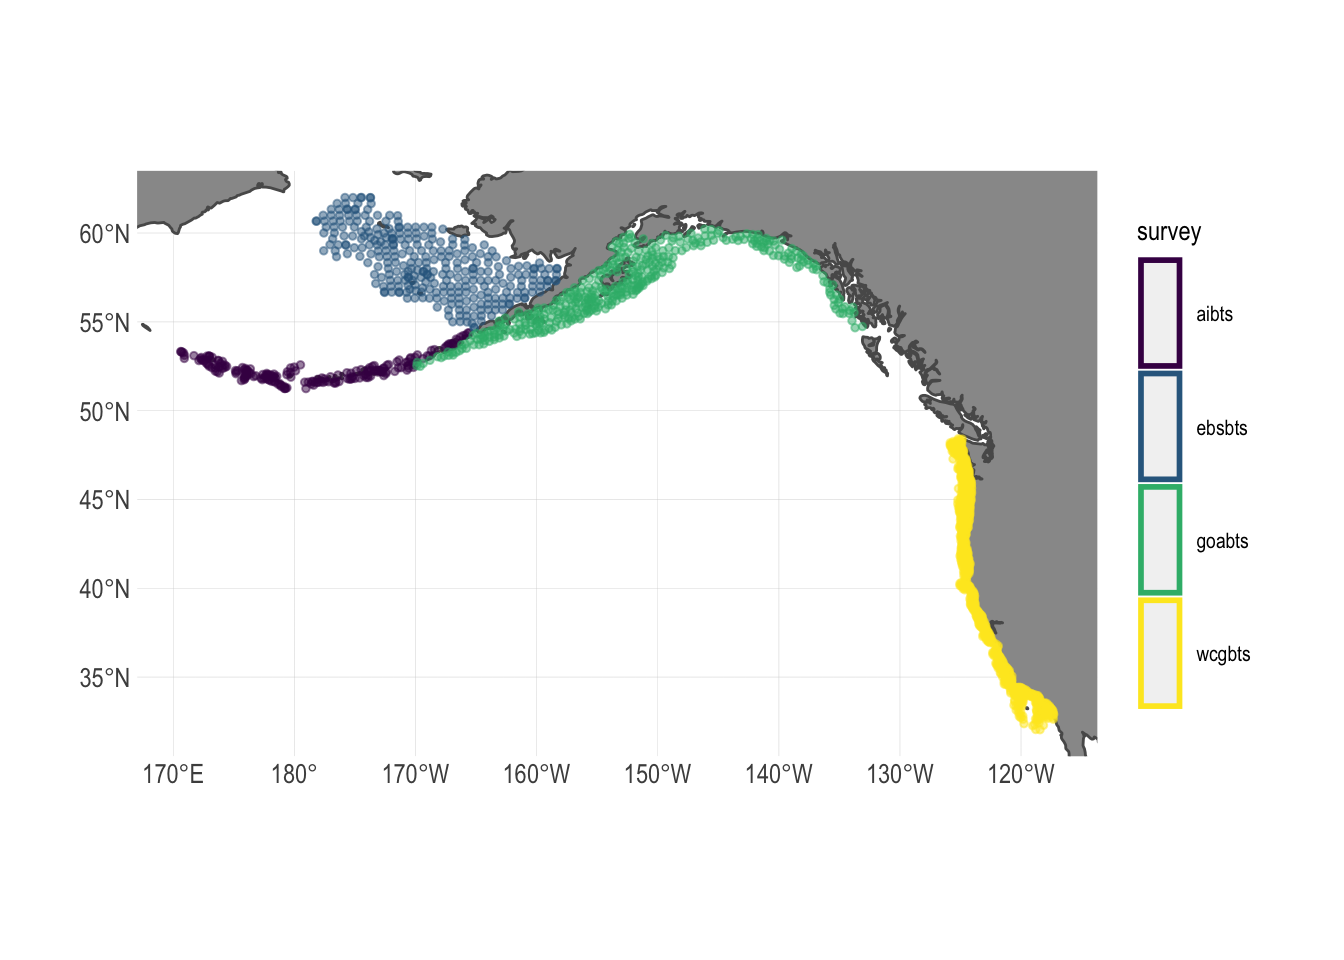
\includegraphics{thesis_files/figure-latex/knot-map-1.pdf}
\caption{\label{fig:knot-map}Spatial coverage of fishery independent
research surveys used in this study. Names represent abbreviated survey
regions}
\end{figure}
Each of the surveys contains data on a wide variety of different
species, including highly abundant fished species such as Arrowtooth
Flounder (\emph{Atheresthes stomias}) and Alaska Pollock (\emph{Gadus
chalcogrammus}), as well as unfished species such as miscellaneous sea
anemones (order \emph{Actiniaria}). The selected surveys utilize bottom
trawl gear, and as such primarily contain bottom-associated species
(Fig.\ref{fig:fish-plot}). Surveys are conducted in summer months
(July-August for the Alaska surveys and May-October for the West Coast
Bottom Trawl Survey).
\begin{figure}
\centering
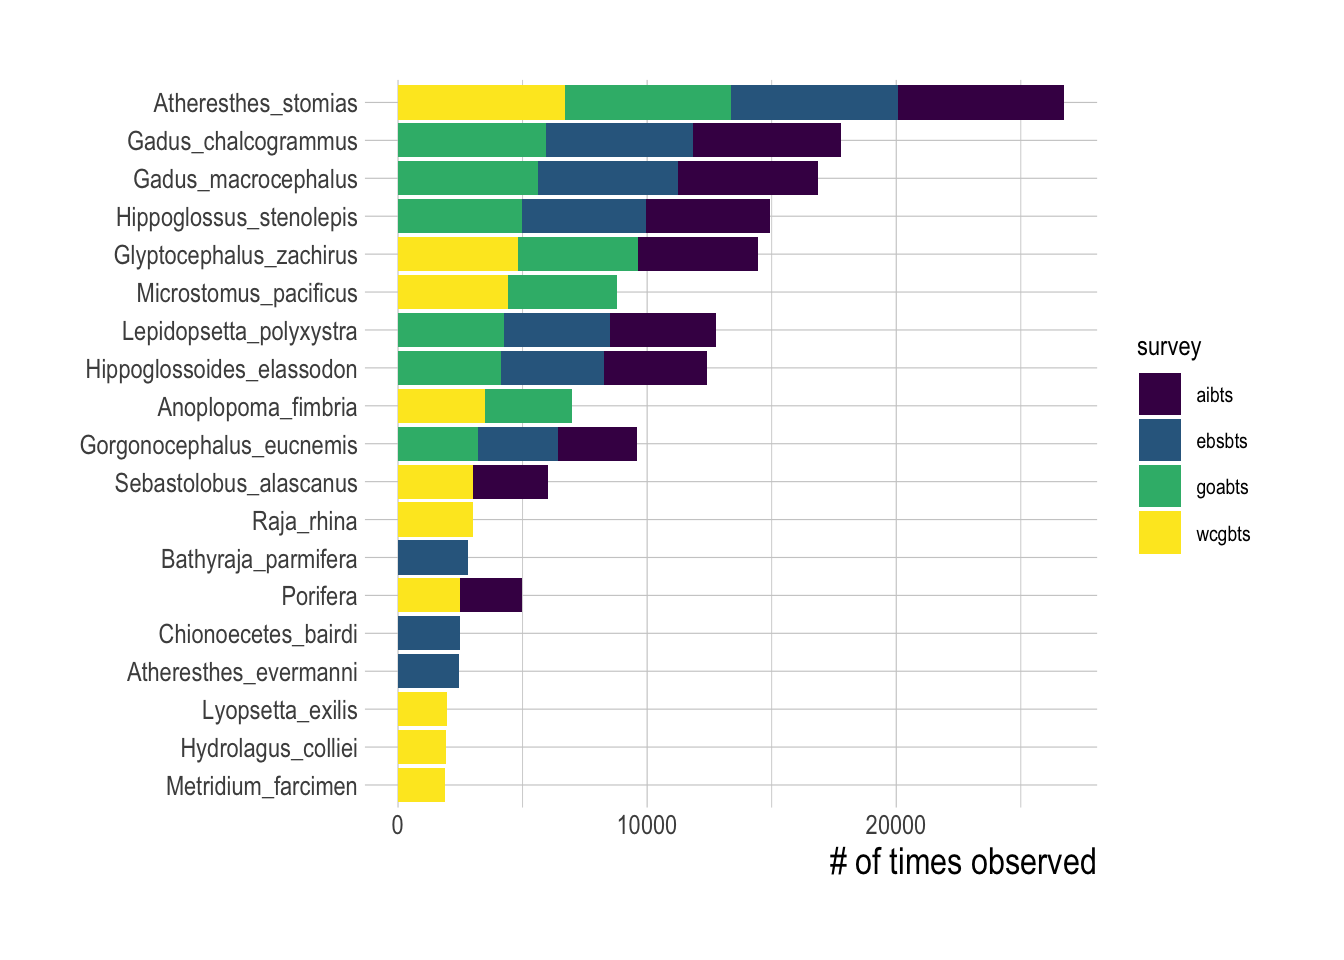
\includegraphics{thesis_files/figure-latex/fish-plot-1.pdf}
\caption{\label{fig:fish-plot}Number of positive encounters for the top-10
most observed species in each research survey}
\end{figure}
Survey data are provided by \texttt{FishData} in their ``raw'' form
(biomass by species per unit of survey effort at a given sampling
event). The data therefore require standardization to account for
differences in vessel characteristics, spatio-temporal correlation
structures, and the presence of zeros in the haul data. This
standardization was performed using the
\href{https://github.com/James-Thorson/VAST}{\texttt{VAST}} package
(Thorson \emph{et al.} \protect\hyperlink{ref-Thorson2016a}{2016}),
which implements a spatial delta-generalized linear mixed model to
provide a standardized spatio-temporal index of abundance for each
species in the data. While versions of \texttt{VAST} allow for
accounting of both within and across species correlations, we chose to
run the standardization process separately for each species for the sake
of convergence time (tests of this choice on smaller subsets of the data
indicate the differences between the two approaches are not
substantial).

The result of VAST is a network of ``knots'' that define polygons of
equal density for each species, where the density of each species is
measured in units of metric tons/km\textsuperscript{2}
(Fig.\ref{fig:fish-map}).
\begin{figure}
\centering
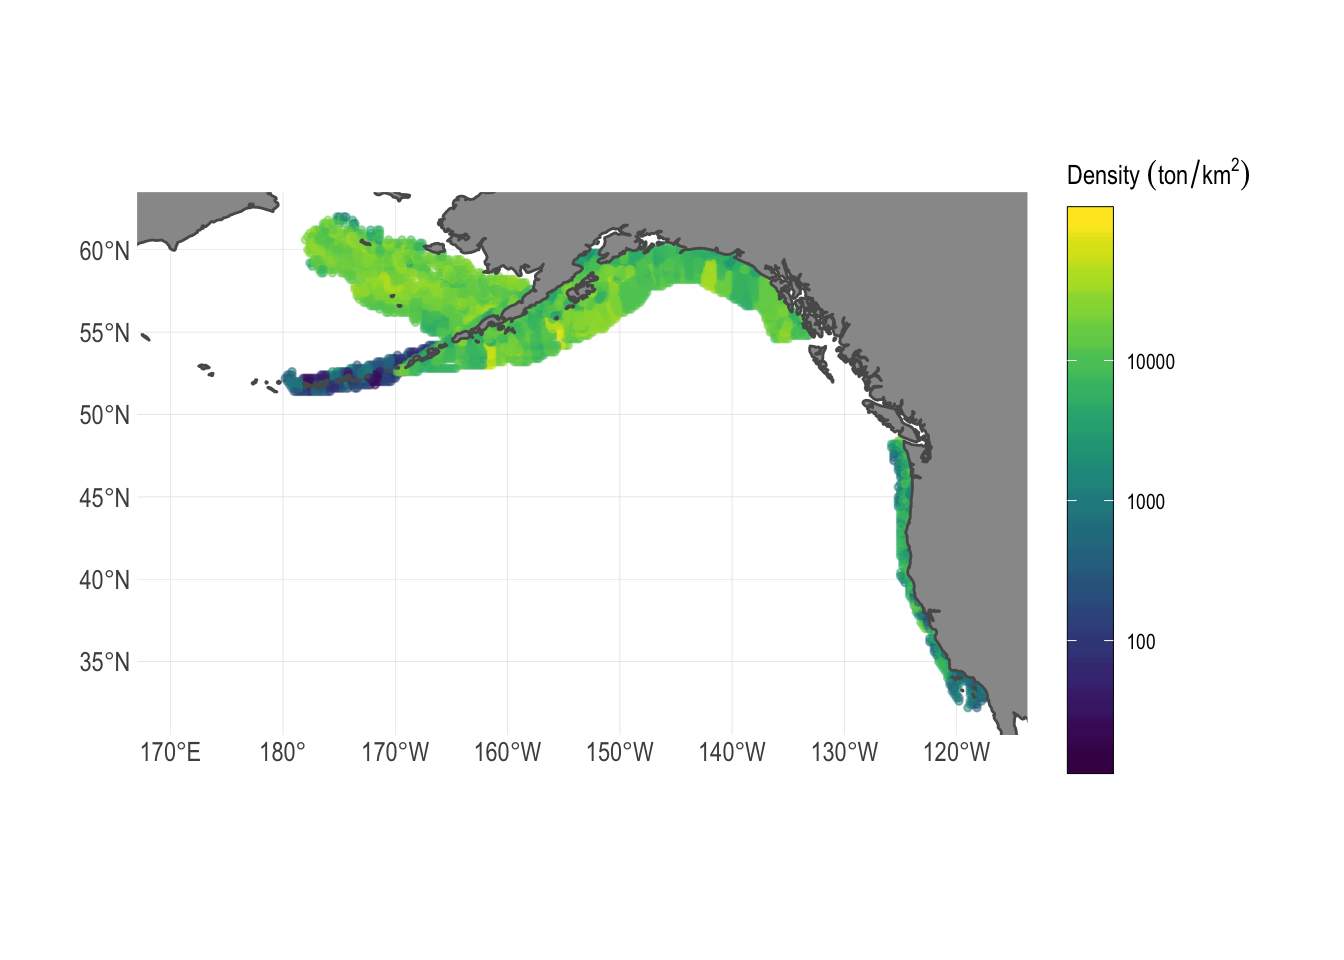
\includegraphics{thesis_files/figure-latex/fish-map-1.pdf}
\caption{\label{fig:fish-map}VAST estimates of density
(tons/km\textsuperscript{2}) of species observed in bottom trawl surveys
for the Alaska region - NOTE seems like problem in reported units of
trawl survey of AIBTS}
\end{figure}
Surveyed species vary substantially in their economic importance. We
mark species encountered in the surveys as ``fished'' if their name, or
a synonym for their name identified through the \texttt{taxize} package,
was found within the global catch records of the Food and Agriculture
Organization of the United Nations (FAO
\protect\hyperlink{ref-FAO2018}{2018}). For each species, we also
obtained price estimates using the data provided by Melnychuk \emph{et
al.} (\protect\hyperlink{ref-Melnychuk2016}{2016}). Together, these data
provide estimated density for fished species encountered by the US west
coast bottom trawl survey program over space and time, along with the
associated value of these species. This allows us to examine both the
density of species, and the ``revenue density'' available for fishing in
different locations (Fig.\ref{fig:price-plot}).
\begin{figure}
\centering
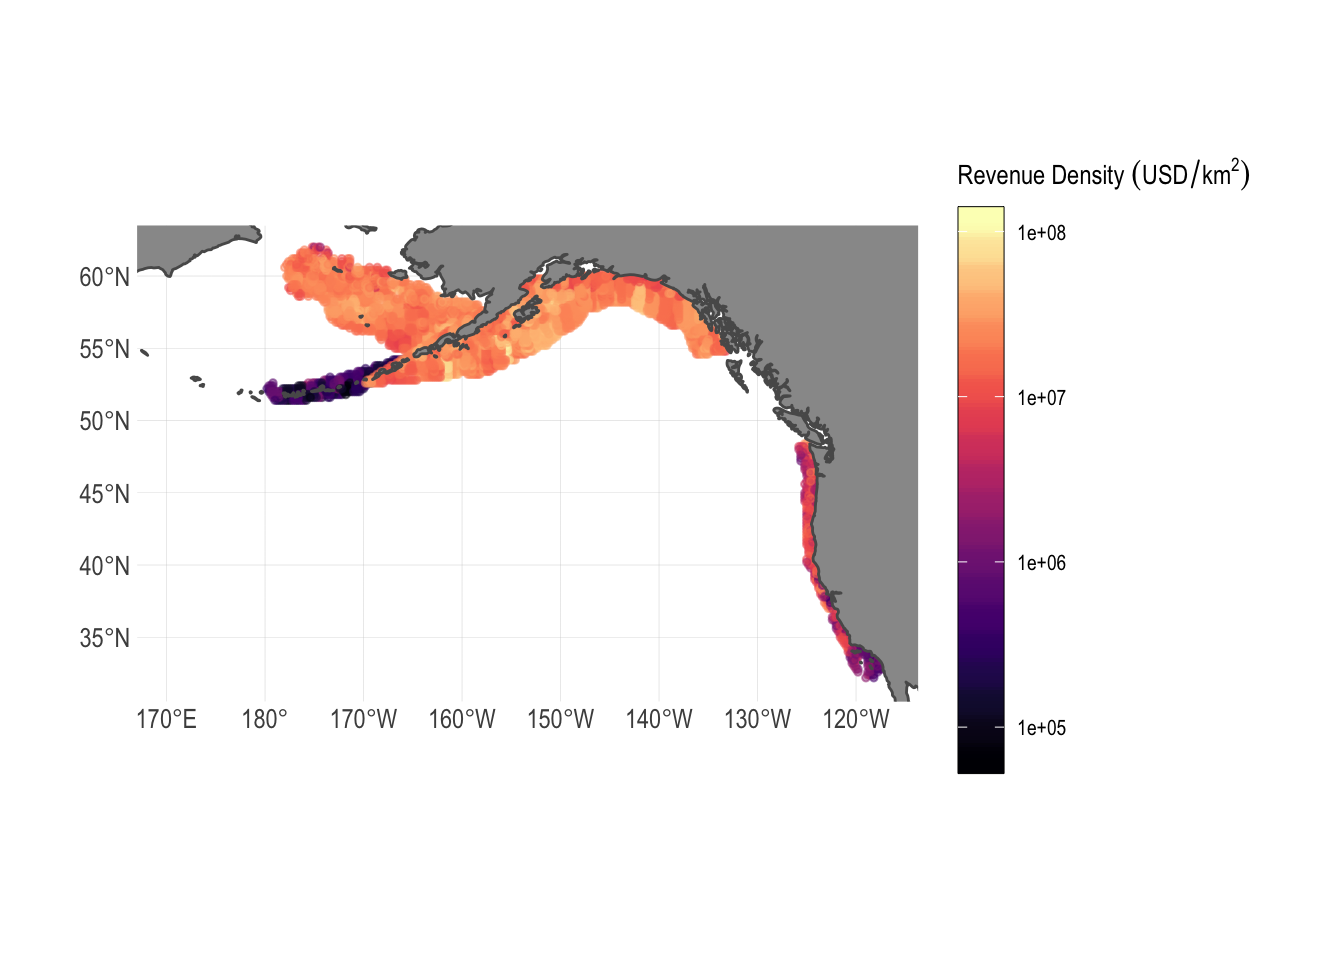
\includegraphics{thesis_files/figure-latex/price-plot-1.pdf}
\caption{\label{fig:price-plot}Estimated fishing revenue density
(\$/km\^{}2)}
\end{figure}
\subsubsection{Fishing Effort Data}\label{fishing-effort-data}

Fishing effort data were obtained using the \texttt{bigrquery} package
in R from Global Fishing Watch. Data were aggregated to the resolution
of year and nearest 0.2 degree latitude and longitude, and for each
vessel at this a given location we calculated the total fishing hours
spent there, average distance from shore, average distance from port,
and whether that location is inside an MPA (and if so whether the MPA
was no-take or restricted-use). We also collected relevant data for that
vessel such as its engine power, length, tonnage, and vessel type
(trawler, purse-seine, fixed-gear, etc). Together, these data provide
fishing effort-related data covering the regions surveyed in our
fishery-independent data (\ref{fig:gfw-map}).

Global Fishing Watch uses a neural-net to classify observed behavior as
fishing or not fishing (Kroodsma \emph{et al.}
\protect\hyperlink{ref-Kroodsma2018}{2018}) From there, we filtered out
the classified fishing behavior to entries that were more than 500m
offshore, were moving faster than 0.01 knots and slower than 20 knots,
to remove likely erroneous fishing entries.
\begin{figure}
\centering
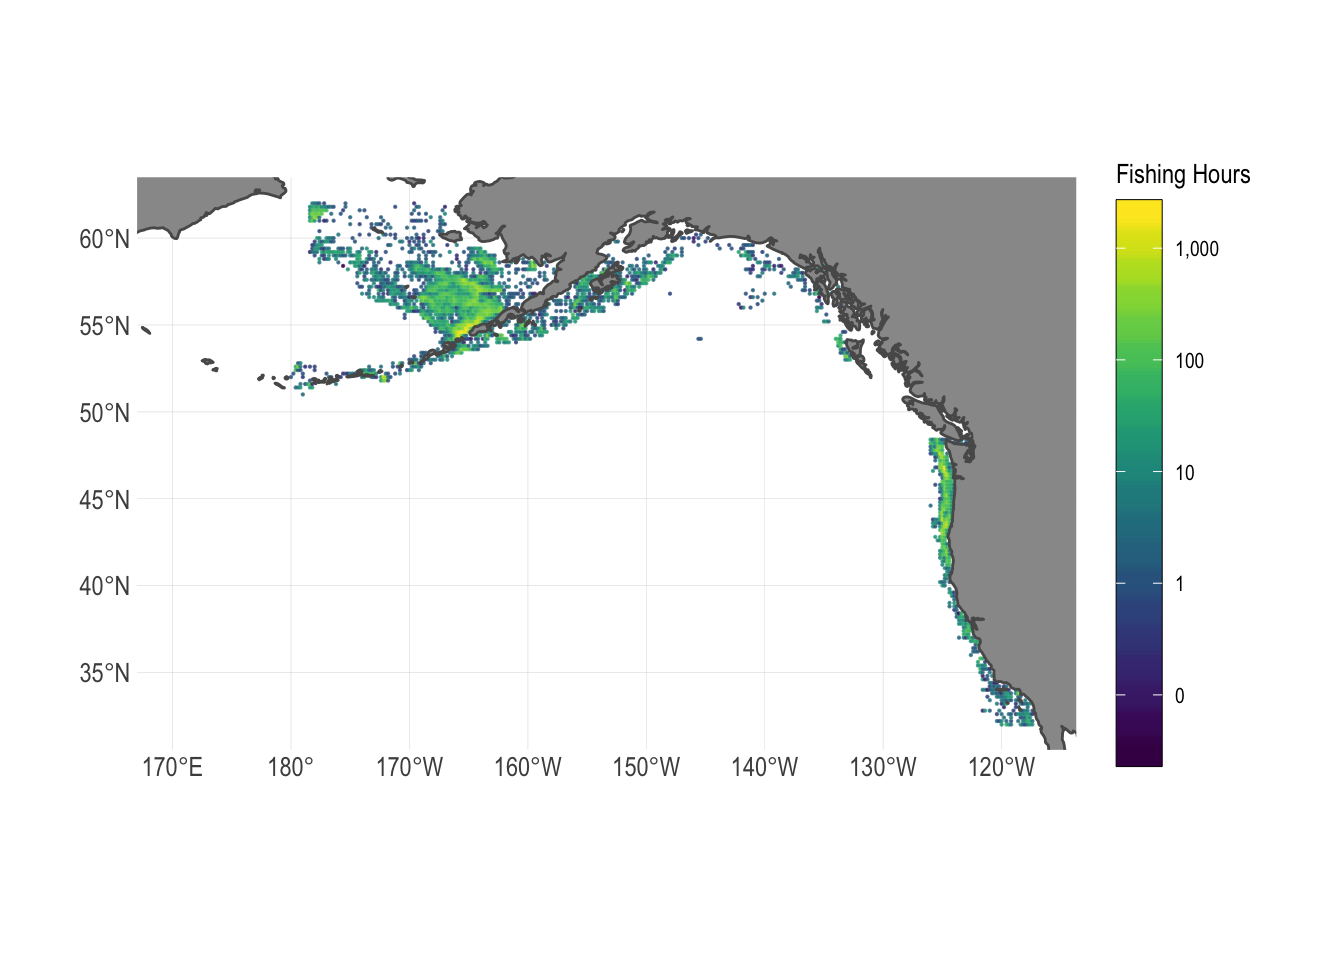
\includegraphics{thesis_files/figure-latex/gfw-map-1.pdf}
\caption{\label{fig:gfw-map}Total hours of fishing activity reported by
Global Fishing Watch in the Eastern Bering Sea, Aluetian Islands, and
Gulf of Alaska regions}
\end{figure}
\subsubsection{Environmental Covariates}\label{environmental-covariates}

We augmented the effort and abundance data with globally accessible
environmental covariates of
\begin{itemize}
\tightlist
\item
  Chlorophyll
\item
  Sea surface temperature
\item
  Bathymetry
\end{itemize}
All data were obtained from
\href{https://coastwatch.pfeg.noaa.gov/erddap/index.html}{NOAA ERDDAP
portal}, and aggregated as needed to match the resolution of the GFW
data (annual and 0.2 degree lat/long resolution). Other environmental
data were explored (e.g.~wave and wind), but did not have sufficient
near-shore coverage for inclusion in the model.

\subsubsection{Creating Merged Database}\label{creating-merged-database}

Having pulled together data on fish abundance, fishing effort, and
environmental covariates, we then merged these data together into a
comprehensive database. Effort data and environmental data were first
merged together by matching year and location (as measured by latitude
and longitude). The combined data were then clipped to only include
observations that fall within the boundaries of the polygons defined by
each trawl survey (Fig.\ref{fig:knot-map}). From there, we snapped each
effort-environment observation to the nearest (in terms of latitude and
longitude distance) knot of fish abundance as defined by the
\texttt{VAST} standardization process. Since the survey data are
generally at a courser resolution than the effort data, this means that
multiple effort observations are often associated with any one knot at
any one time.

We then performed a series of filtering steps on this merged database.
Since all surveys are geared towards bottom dwelling species, only
bottom-associated gears are included from the effort data. In this case
that means vessels identified by Global Fishing Watch as trawlers, pots
and traps, and set gears (bottom longline and gillnet). We also only
included species that were observed 10 or more times during each year of
the survey to improve model convergence. To account for potential
seasonal shifts in abundance, we also filtered the data down to months
in which the relevant research trawl surveys were conducted.

This final merged database provides effort data at the resolution of
effort per 0.2 degree\textsuperscript{2} per year, and abundance at the
resolution of ``knot'' per year, where the exact area of each knot
varies. Each observation of effort is then paired to the spatially
nearest knot of abundance estimates This leaves open a question of at
what resolution do we wish to fit the models? At the temporal scale, we
can only fit to annual data, since that is the temporal resolution of
the abundance estimates. On the spatial scale though, at the finest
resolution we can use a 0.2 degree\textsuperscript{2} spatial
resolution, or we could aggregate all the data up to a total abundance
estimate each year. The challenge here is a trade-off between decreasing
noise but also decreasing degrees of freedom. Since we only have at most
six years of data (and some regions less), aggregating all data together
to the annual scale would leave us with only six datapoints. While we
explore some visual assessments of this idea, six datapoints do not
leave us much room for model fitting. At the other end of the scale,
using the finest resolution data gives us a very large sample size, but
also means we are trying to predict abundances at a very fine spatial
scale. So, even if the goal of the model is to predict time trends, we
still fit the model using finer resolution spatial data, and then
aggregate predictions together if we wish to examine time trends.

\subsection{Candidate Predictive
Models}\label{candidate-predictive-models}

We evaluated three classes of candidate models for linking fishing
effort to fish abundance:
\begin{enumerate}
\def\labelenumi{\arabic{enumi}.}
\tightlist
\item
  Linear models
  \begin{itemize}
  \tightlist
  \item
    These simply link abundance to effort through linear models.
  \end{itemize}
\item
  Structural economic models
  \begin{itemize}
  \tightlist
  \item
    These assume a non-linear functional form to the allocation of
    fishing effort, the parameters of which are tuned to available data
    conditional on these structural assumptions.
  \end{itemize}
\item
  Machine learning models
  \begin{itemize}
  \tightlist
  \item
    These models make no explicit structural assumptions, but rather
    find the combination of predictor variables that maximize the
    out-of-sample predictive power of the model
  \end{itemize}
\end{enumerate}
The choice of evaluating both structural and machine learning models is
important to discuss for a moment. Substantial amounts of empirical
evidence and bio-economic theory exists hypothesizing how fishing effort
and fish abundance might be related, from relatively classical
ideal-free distributions (e.g. Miller and Deacon
\protect\hyperlink{ref-Miller2016}{2016}) to more complex agent-based
approaches (e.g. Vermard \emph{et al.}
\protect\hyperlink{ref-Vermard2008}{2008}). These structural models have
the advantage of interpretability, but leave us open to errors in model
specification. In contrast, machine learning models lose
interpretability but are less sensitive to specification errors. While
different in their mechanics, all the candidate machine learning models
are black-box models whose sole objective is to maximize the predictive
power of the model (as defined by the user). The user specifies some
model options, but the model decides which data are important and how
those data relate to each other. This allows these algorithms to fit
highly non-linear models (if the data demand it), without the need to
specify an exact statistical or structural form for how variables such
as costs, safety, and fish abundance interact to affect fishing
behavior.

As a result, machine learning models can serve as an effective benchmark
for the best possible ability of GFW data to predict fish abundance. The
disadvantage is that, while new techniques are emerging for interpreting
machine learning model fits, they are inherently black boxes and as such
do not permit us to really interpret the meaning of specific
coefficients. The lack of a structural theory behind the model may also
hamper the ability of these models to predict radically out of sample
data (e.g.~a machine learning model trained in Alaska may perform
terribly in Africa). By fitting both structural and machine learning
models, we can compare the machine learning and structural approach and
see how much the interpretability of the structural model ``costs'' us
in terms of predictive power, relative to the benchmark of the machine
learning model.

\subsection{Linear Models}\label{linear-models}

We include the linear models purely for data exploration (though if they
happen to work well they could be used). The linear models include
simple linear regressions between metrics of effort and metrics of
abundance (e.g.~total engine hours against total biomass). We also
consider CPUE trends as a class of linear model (since it is just a
linear transformation of the effort data), where we now ask is, is a
Global Fishing Watch index of CPUE proportional to abundance? We tested
one slightly more involved linear model, of the form

\[(E_{y,k}) \sim Gamma(cost_{y,k} + \hat{B_{y,k}}, shape, scale)\]

\[ \hat{B_{y,k}} \sim normal(\bar{B_{survey}}, \sigma_{survey})\]

Where \(E_{y,k}\) is the observed total effort in year \emph{y} for knot
(location) \emph{k}, \emph{cost} is our linear cost function, and
\(\hat{B}\) is a estimate of the effect for each knot, drawn from a
distribution within each survey with mean \(\bar{B_{survey}}\). In order
for \(\hat{B}\) to in fact be representative of fish biomass at a
location, the assumption is that all of the other attributes that affect
the decision of how much effort to allocate at a given site are captured
by the estimated cost coefficient, which we assume is a linear function
of the distance of a knot \emph{k} from port, the distance from shore,
the depth at that location, and the mean vessel size used at that
observation. We used a Bayesian hierarchical model implemented through
the \texttt{rstanarm} package to estimate this linear model. We then
extracted the estimated \(\hat{B}\) coefficients, and compared them to
the fish biomass estimated at that location by the relevant fishery
independent survey.

\subsection{Structural Models}\label{structural-models}

Our structural models are constructed in the same manner as Miller and
Deacon (\protect\hyperlink{ref-Miller2016}{2016}). The key of this model
is the assumption that for a given spatio-temporal resolution, fishermen
distribute themselves such that marginal profits are equal in space.

Following Miller and Deacon (\protect\hyperlink{ref-Miller2016}{2016}),
we consider marginal profits \(\Pi\) per unit effort as being

\[\Pi_{y,k} = pqB_{y,k}e^{-qE_{y,k}} - c_{y,k}\]

where for year \emph{y} at knot \emph{k}, \emph{p} is price (drawn from
Melnychuk \emph{et al.} \protect\hyperlink{ref-Melnychuk2016}{2016}),
\emph{B} is our index of abundance (from the trawl surveys and VAST),
\emph{q} is catchability, \emph{E} is effort (supplied by Global Fishing
Watch), and \emph{c} are variable costs).This leaves \emph{q} and
\emph{c} as the unknowns in this equation.

Miller and Deacon (\protect\hyperlink{ref-Miller2016}{2016}) were
primarily interested in estimating quota price aspects of \emph{c},
taking as data \emph{p}, \emph{CPUE}, \emph{E}, and other components of
\emph{c} (fuel, labor, ice, etc.). We are instead interested in
estimating CPUE as a function of other variable, and so we can rearrange
this equation to construct a model of the form

\[log(B_{y,k}) \sim normal(\frac{\Pi_{y,k} + c_{y,k}}{pqe^{-qE_{y,k}}}, \sigma_B)\]

Similar to Miller and Deacon (\protect\hyperlink{ref-Miller2016}{2016})
we assume for now that \(\Pi_{y,k}\) is zero, though this is clearly not
accurate given that many of the fisheries encompased by the data are
highly regulated and in some cases rationalized (however, changing
\(\Pi_{y,k}\) to positive values had little effect on the fit of the
model during trial runs). That leaves \emph{q} and \emph{c} as unknown
parameters. While we do not have the high resolution logbook data
available to Miller and Deacon
(\protect\hyperlink{ref-Miller2016}{2016}), we could certainly obtain
data on fuel and labor prices for this model. However, at this time, we
simply assume that \(c_{y,k}\) is a linear function of the distance of a
knot \emph{k} from port, the distance from shore, the depth at that
location, and the mean vessel size used at that observation. We fit this
model, estimating \emph{q} and the cost coefficients and \(\sigma_B\)
using maximum likelihood with the Laplace approximation implemented with
Template Model Builder (TMB, Kristensen \emph{et al.}
(\protect\hyperlink{ref-Kristensen2016}{2016})) in R.

This form of the model assumes the goal is to estimate \emph{B}
directly. Use of this model for prediction in new locations would
require assuming that the fitted \emph{q} and \emph{cost} values are
applicable to a new location. An alternative approach is to estimate a
vector of latent variables \(\hat{B}\) that, together with the
\emph{cost} and \emph{q} estimates explain the observed effort
distribution.

\[E_{y,k} \sim Gamma(\frac{1}{q}log(\frac{pq\hat{B_{y,k}}}{c_{y,k} + \Pi_{y,k}}), shape, scale)\]

\[ \hat{B_{y,k}} \sim normal(\bar{B_{survey}}, \sigma_{survey})\]

This form of the model can be custom fit to any new region, but requires
the assumption that all of the non-biomass related reasons for fishing
at a given site are captured by the fitted \emph{cost} coefficients,
leaving the ``biomass'' effect to be captured by the latent variables.
If there are other site specific factors that affect the amount of
fishing effort and are not included in the model though, these factors
will get soaked up by \(\hat{B_{y,k}}\), confounding the interpretation
of these fitted latent values as biomass indicators. We fit this model
as a Bayesian hierarchichal model using the \texttt{brms} (Bürkner
\protect\hyperlink{ref-Burkner2017}{2017}) interface to Stan (Carpenter
\emph{et al.} \protect\hyperlink{ref-Carpenter2017}{2017}) in R.

\subsection{Machine Learning}\label{machine-learning}

We implemented four machine learning algorithms:
\begin{itemize}
\tightlist
\item
  random forests (implemented through the \texttt{ranger} package in R)
\item
  generalized boosted regression modeling (\texttt{gbm})
\item
  boosted multivariate adaptive regression splines (\texttt{bmars})
\item
  multivariate adaptive regression splines (\texttt{mars})
\end{itemize}
An important feature across all the machine learning approaches is that
they all adaptively push back against predictive overfitting. Within the
training data split, the machine learning approaches then split the
training data into numerous new testing and training splits (typically
now called assessment and analysis splits). The coefficients of the
model are then in part fit by repeatedly searching subsets of parameters
that minimize the predictive error of the model trained on the analysis
split. Tuning parameters can be selected by comparison of predictive
error of fitted models applied to the assessment splits. This process is
repeated thousands of times the algorithms search for coefficients that
while fitted on one set of data still provide reasonable predictive
power on a held out set of data.

A random forest works by fitting a series of regression trees. Each
regression tree takes a sub-sample of the training data, and a sub
sample of the independent variables provided for model fitting. The
algorithm then determines the variable and variable split (e.g.~vessel
size and vessel size above 30ft) that provides the greatest explanatory
power for the sampled data, and creates that as the first node. The next
two nodes are selected in the same process, and so on and so forth, down
to a specified tree depth tuned through the \texttt{caret} package. Each
tree provides a high-variance, low bias estimator of densities. The
random forest then averages over hundreds of trees to reduce this
variance and provide an improved estimate of density as a function of
provided covariates. The advantage of this approach is that it makes no
assumptions about error distributions or linearity of parameters, and
the process of randomly sampling both data and predictors actively
pushes back against overfitting (Breiman
\protect\hyperlink{ref-Breiman2001}{2001}). Despite the starkly
different name, a GBM is more or less a modification of a random forest
that helps the model target and improve the fit of parts of the data
that the model struggles with. It does this by for each split,
calculating the residuals, and then adapting the model fit to target
parts of the data with large residuals.

Multivariate adaptive regression splines (MARS) models exploit similar
assessment-analysis tools as random forest, but rather than working by
splitting the data into a series of discrete bins that form a tree, the
model breaks the data and variables into an ensemble of linear
regressions. For example, consider a process \emph{f} that takes an
independent variable \emph{x} and a dependent variable \emph{y}, that
can be modeled by two linear models: when \emph{x} is 1:10 \emph{y}
\textasciitilde{} f(0.1\emph{x}), and when \emph{x} is 11:20 y
\textasciitilde{} f(0.5\emph{x}). A properly tuned MARS model will
search through the data, notice the split, and fit two different linear
regressions to each component of the data. Similarly to the random
forest model, the MARS model considers subsets of available variables
and possible levels of interaction among these variables. The
``boosted'' version of this model targets hard-to-fit parts of the model
in the same was as the GBM model.

Unlike more classic fitting procedures, for example considering a GAM vs
a GLM, there is little \emph{a priori} reason to consider one type of
machine learning models over another. They all have been shown to work
well under different circumstances, and so the selection process often
simply comes down to selecting some reasonable candidates, fitting them,
and then selecting the best model from the fits to the training data
based on the user's criteria.

\section{Results}\label{results}

\subsection{Linear Models}\label{linear-models-1}

Before heading down the statistical rabbit hole, we can simply examine
how well linear transformations of effort predict abundance. This has an
intuitive aspect to it; we can hypothesize that the reason that more
fishing occurs in the challenging waters off Alaska than Santa Barbara
is that there are higher volumes of valuable fish in that area. However,
we could also imagine a scenario where fishing effort is concentrated in
overfished but inexpensive grounds, leaving higher fish abundance in
more remote areas that are not economical to fish.

Looking at the effort and abundance indices, we see some evidence of a
``more fishing where there are more fish'' hypothesis. Across each of
the survey regions, aggregating up to a 100 km\textsuperscript{2} area,
there is a positive correlation between the total engine hours of
applicable fishing observed by GFW in that area and the total estimated
fishable biomass available in that area (estimated by the sum of the
density per knot times the area of that knot). However, the relationship
is far from clear, with substantial variation around the mean slope for
each region. In addition, we see if all one knew was the total amount of
fishing hours, the magnitude of the fishing opportunity that those hours
might correspond to varies substantially (Fig.\ref{fig:effort-v-fish}).
\begin{figure}
\centering
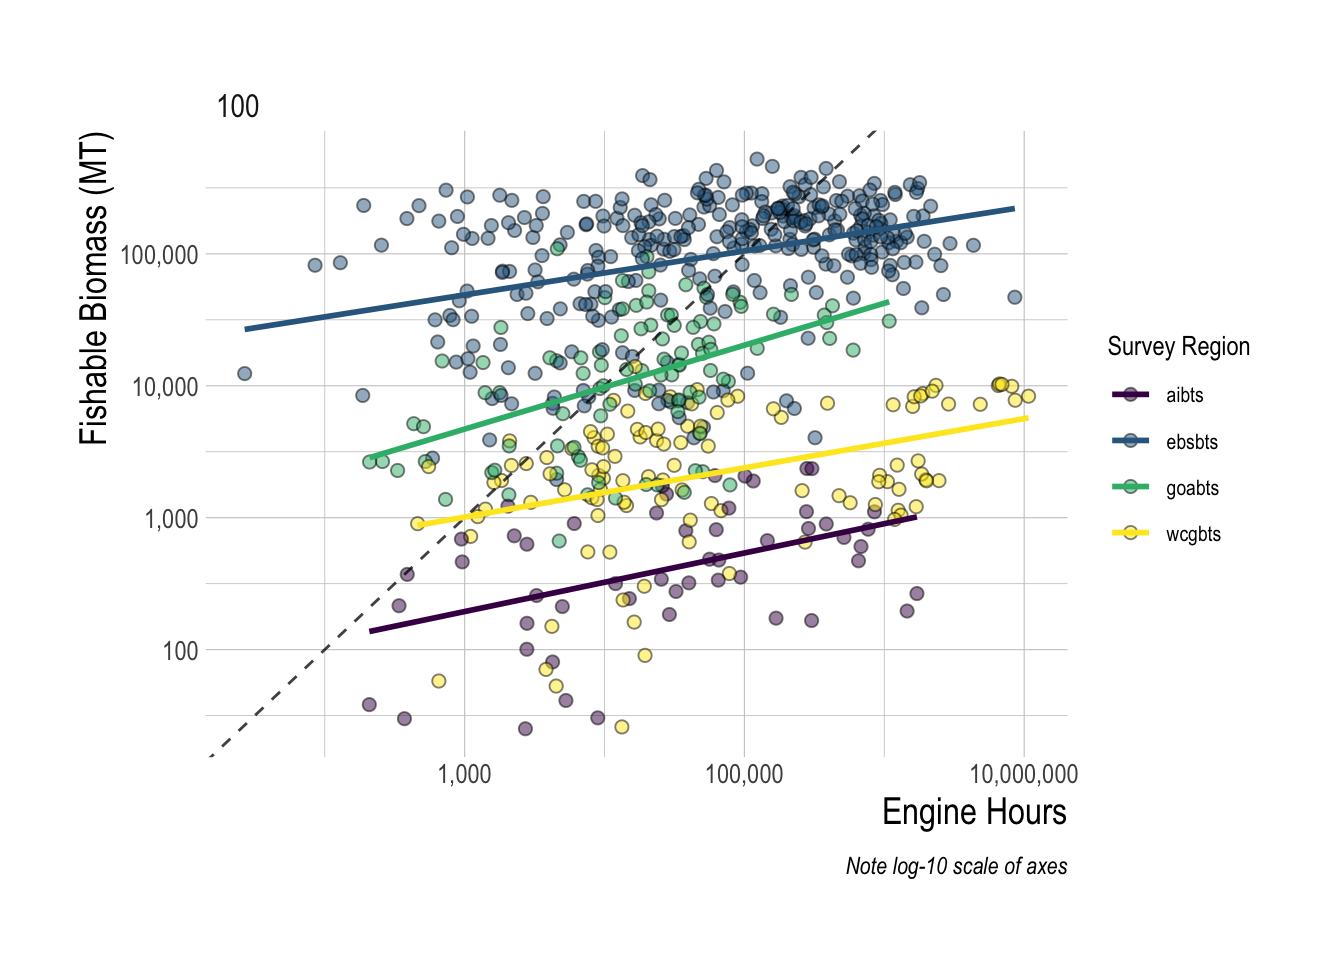
\includegraphics{thesis_files/figure-latex/effort-v-fish-1.pdf}
\caption{\label{fig:effort-v-fish}Total fishing hours plotted against fish
revenue density. Available revenue is calculated as the sum of the
densities of each species times their respective ex-vessel price. Each
point represents a 200km\textsuperscript{2} area}
\end{figure}
This coarse data analysis suggests that there may be a relationship
between total fishing effort and the value of the fishing opportunity
within a region, but certainly not a clear enough relationship to serve
as a reliable predictor of fishable biomass. That effort levels alone
are not clearly informative is not very surprising. What though do we
learn by pairing effort data with locally available catch data to
construct a CPUE index? CPUE can, under the appropriate circumstances,
serve as an index of relative abundance (Maunder \emph{et al.}
\protect\hyperlink{ref-Maunder2006}{2006}), though it can also fail
badly at this task if key assumptions are violated (Hilborn and Kennedy
\protect\hyperlink{ref-Hilborn1992a}{1992}; Harley \emph{et al.}
\protect\hyperlink{ref-Harley2001}{2001}; Walters
\protect\hyperlink{ref-Walters2003}{2003}). Ignoring complications in
interpretation of CPUE for now, to create a GFW derived CPUE index, we
pulled catch data for the relevant regions and species from three
different databases: the RAM Legacy Stock Assessment Database (Ricard
\emph{et al.} \protect\hyperlink{ref-Ricard2012}{2012}), the
\href{https://www.st.nmfs.noaa.gov/commercial-fisheries/commercial-landings/annual-landings/index}{NMFS
commercial landings database}, and the FAO's capture production database
(FAO \protect\hyperlink{ref-FAO2018}{2018}). Pairing these catch data
with the the GFW effort data gives us a timeseries of aggregate CPUE for
a given region. We then compared these CPUE trends to trends in biomass
provided by the RAM database and from the processed trawl survey used
throughout this study. In the Eastern Bering Sea region, if you squint
there appears to be some a shared downward trend since 2014 between the
CPUE indices and the independent abundance indices
(Fig.\ref{fig:ebs-cpue}). But, the GFW derived CPUE indices tell the
exact opposite story as the independent abundance indices along the US
West Coast (Fig.\ref{fig:wc-cpue}).
\begin{figure}
\centering
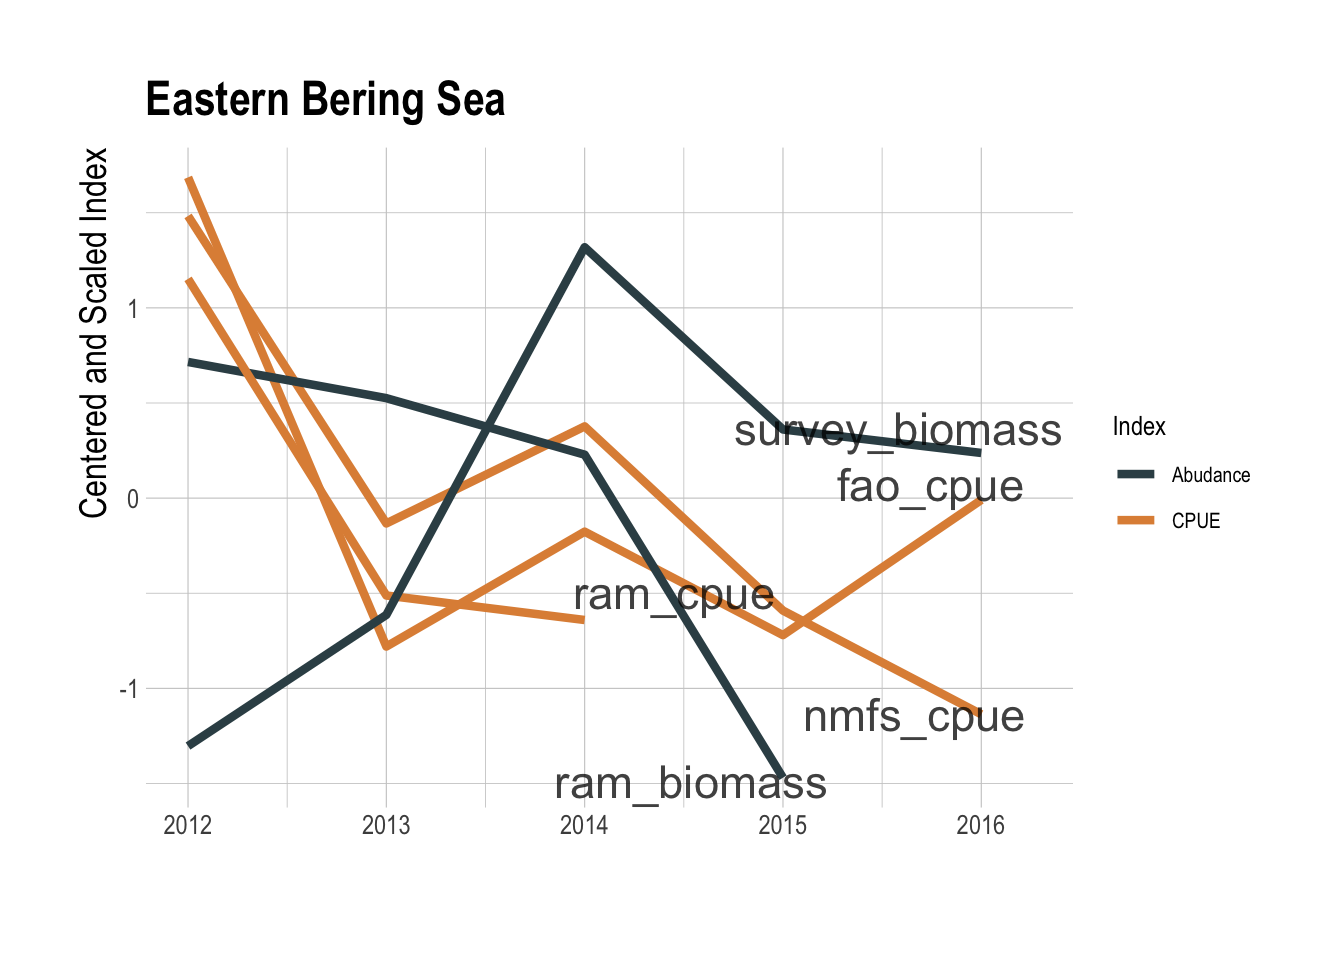
\includegraphics{thesis_files/figure-latex/ebs-cpue-1.pdf}
\caption{\label{fig:ebs-cpue}GFW derived CPUE (orange) and assessments of
abundance (blue) for the Eastern Bering Sea region}
\end{figure}
\begin{figure}
\centering
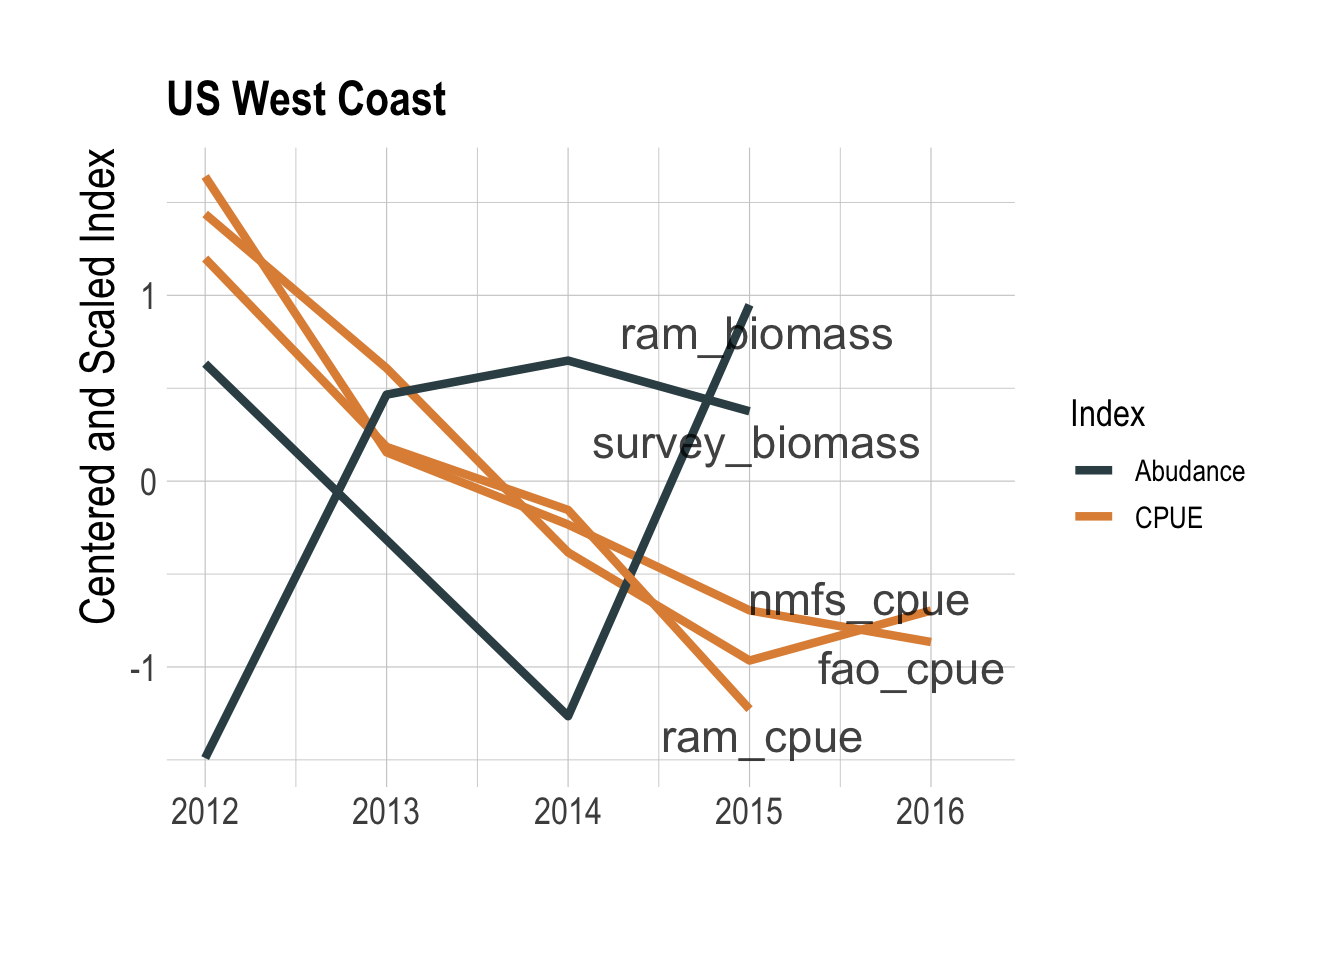
\includegraphics{thesis_files/figure-latex/wc-cpue-1.pdf}
\caption{\label{fig:wc-cpue}GFW derived CPUE (orange) and assessments of
abundance (black) for the US West Coast}
\end{figure}
Turning to the latent variables approach for the linear models, We find
no correspondence between the estimated space effects \(\hat{B}\) and
the fish biomass estimated from the trawl surveys. This does not mean
that such an approach might not work given sufficient data, but with the
available covariates either omit too many other important factors
besides biomass are being absorbed into the \(\hat{B}\) coefficients, or
the survey biomass is a small component of the decision making process
for a given fishing location (Fig.\ref{fig:linear-latent-plot}).
\begin{figure}
\centering
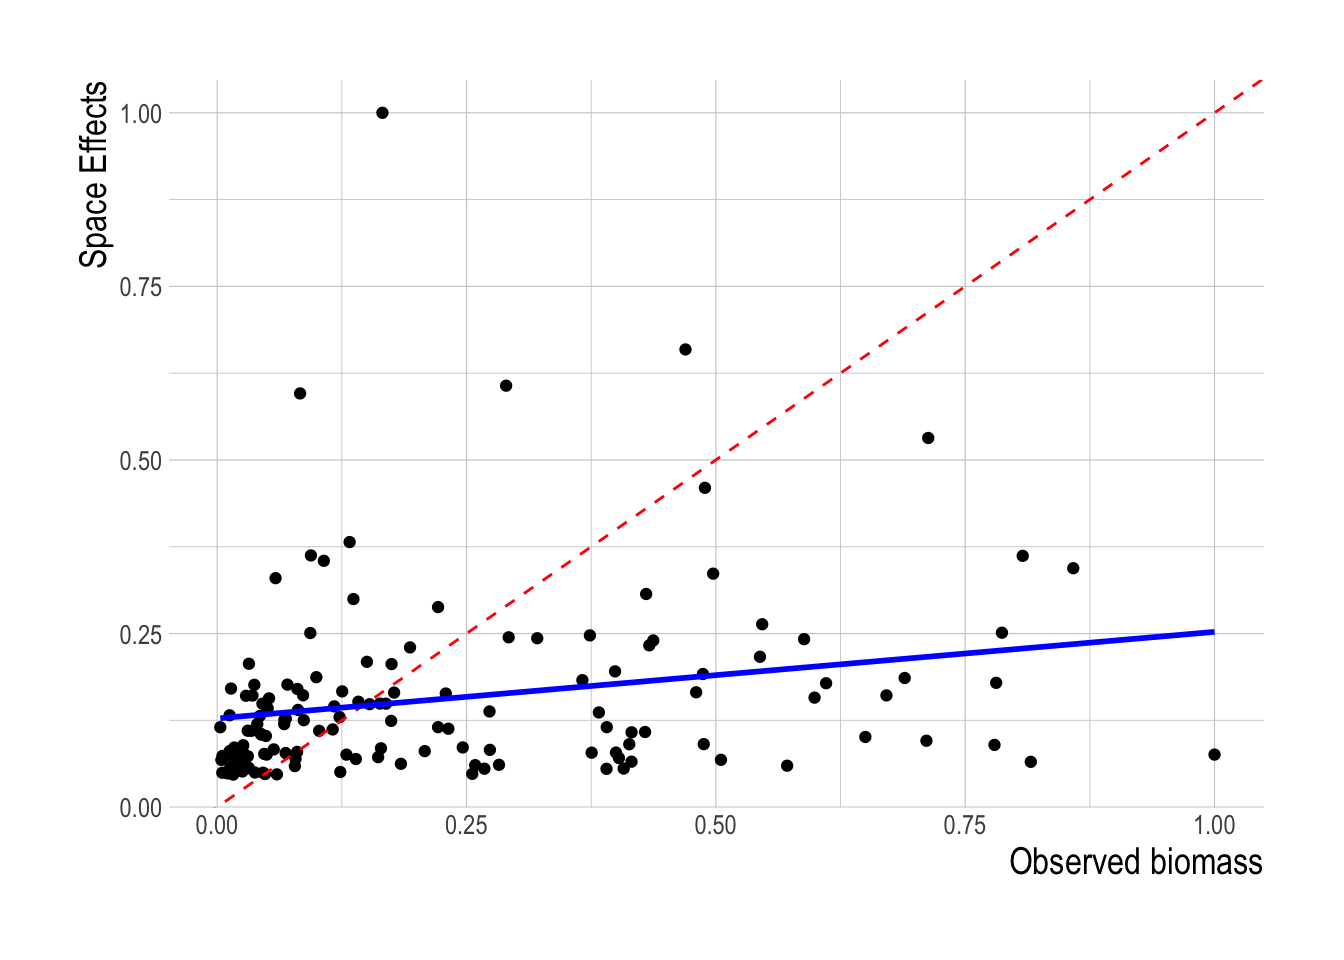
\includegraphics{thesis_files/figure-latex/linear-latent-plot-1.pdf}
\caption{\label{fig:linear-latent-plot}Scaled latent biomass coefficients
plotted against paired scaled biomass estimates. Red dashed line
indicates a 1:1 fit, solid blue line represents a linear model of the
two axes}
\end{figure}
\subsection{Structural Models}\label{structural-models-1}

Since raw effort and effort derived CPUE indices do not appear to be
valid methods for estimating abundance, we now turn to more detailed
modeling approaches to utilize effort data to predict abundance. Our
structural modeling approach follows a standard bio-economic framework,
as laid out in Miller and Deacon
(\protect\hyperlink{ref-Miller2016}{2016}). Miller and Deacon
(\protect\hyperlink{ref-Miller2016}{2016}) used a structural modeling
approach in part to estimate the quota prices in the US West Coast
groundfish trawl fishery individual fishing quota (IFQ) program, using
data on logbook reported CPUE, prices, and variable and fixed costs
(labor, fuel, etc.). Making the assumption that for an appropriate fleet
unit and time period marginal profits are equal in space, Miller and
Deacon (\protect\hyperlink{ref-Miller2016}{2016}) then estimate quota
prices for different species that, given their other data, rationalize
the observed distribution of effort in the fishery. We applie this same
theory to our data, but rearranging the equation so that the model now
estimates biomass rather than effort. This biomass-predicting structural
model shows limited predictive ability within the training set, with
R\textsuperscript{2} within the training data less of 0.13.
\begin{figure}
\centering
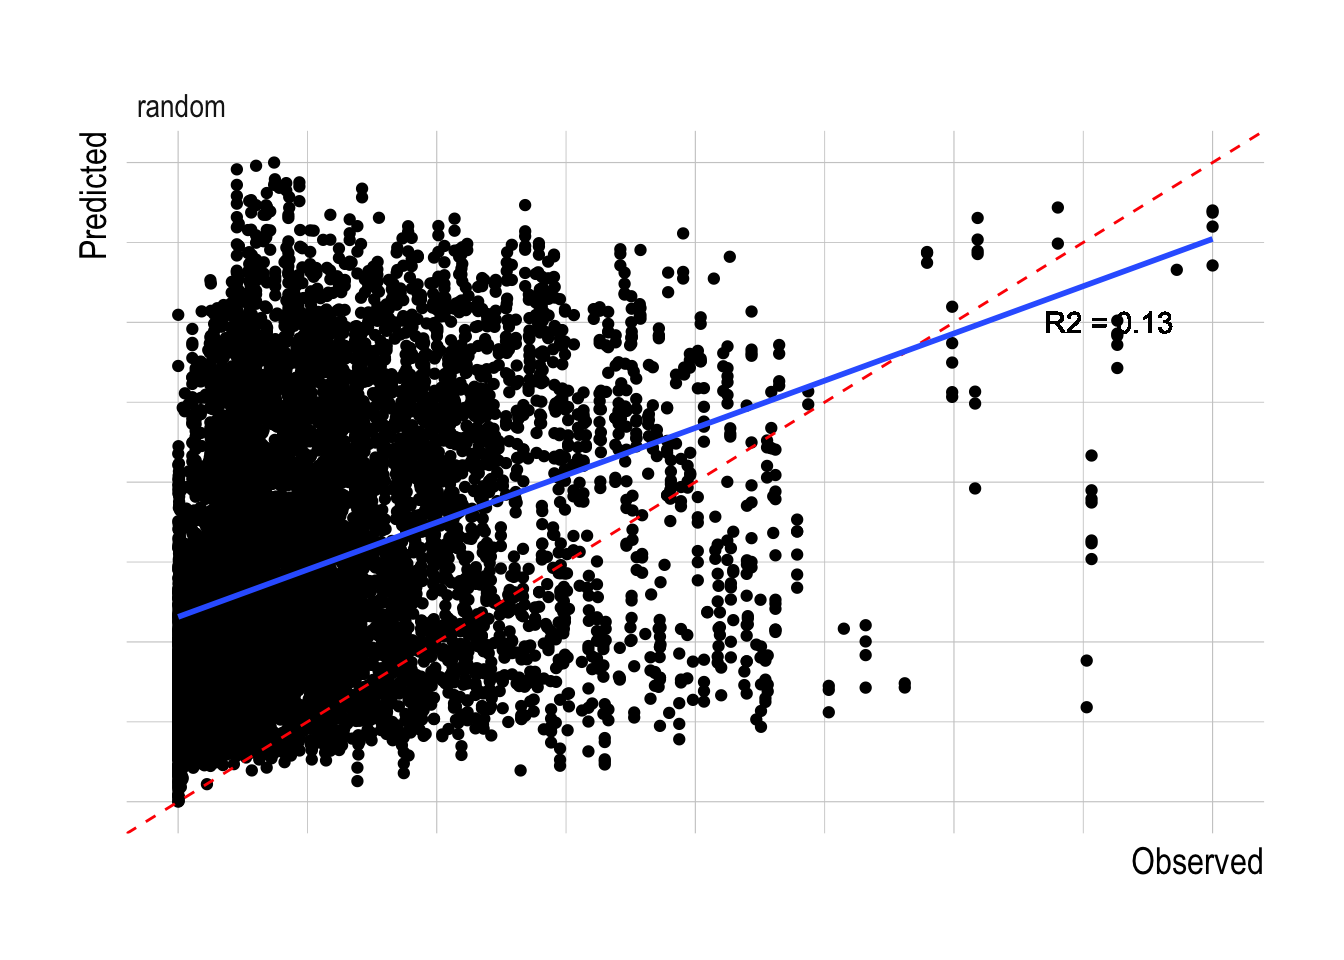
\includegraphics{thesis_files/figure-latex/strct-ovp-plot-1.pdf}
\caption{\label{fig:strct-ovp-plot}Observed vs predicted biomass (A) and R2
values (B) for the fitted structural model. Red dashed line shows 1:1
relationship, blue line a fitted linear model to the observed and
predicted values}
\end{figure}
We can also inverted this idea in the same manner as we did with the
linear model, and rather than estimating cost coefficients that explain
the observed fish abundance, given observed efforts, estimate cost
coefficients and latent spatial parameters representing abundance that
explain the observed effort. We estimated this model using a Bayesian
hierarchical model implemented in \texttt{brms} (rather than
\texttt{rstanarm} since the model is no longer linear). Similarly to the
linear model exercise, we found no relationship between the estimated
latent spatial abundance coefficients and the estimates of fish
abundance provided by the trawl surveys
(Fig.\ref{fig:strct-latent-plot}).
\begin{figure}
\centering
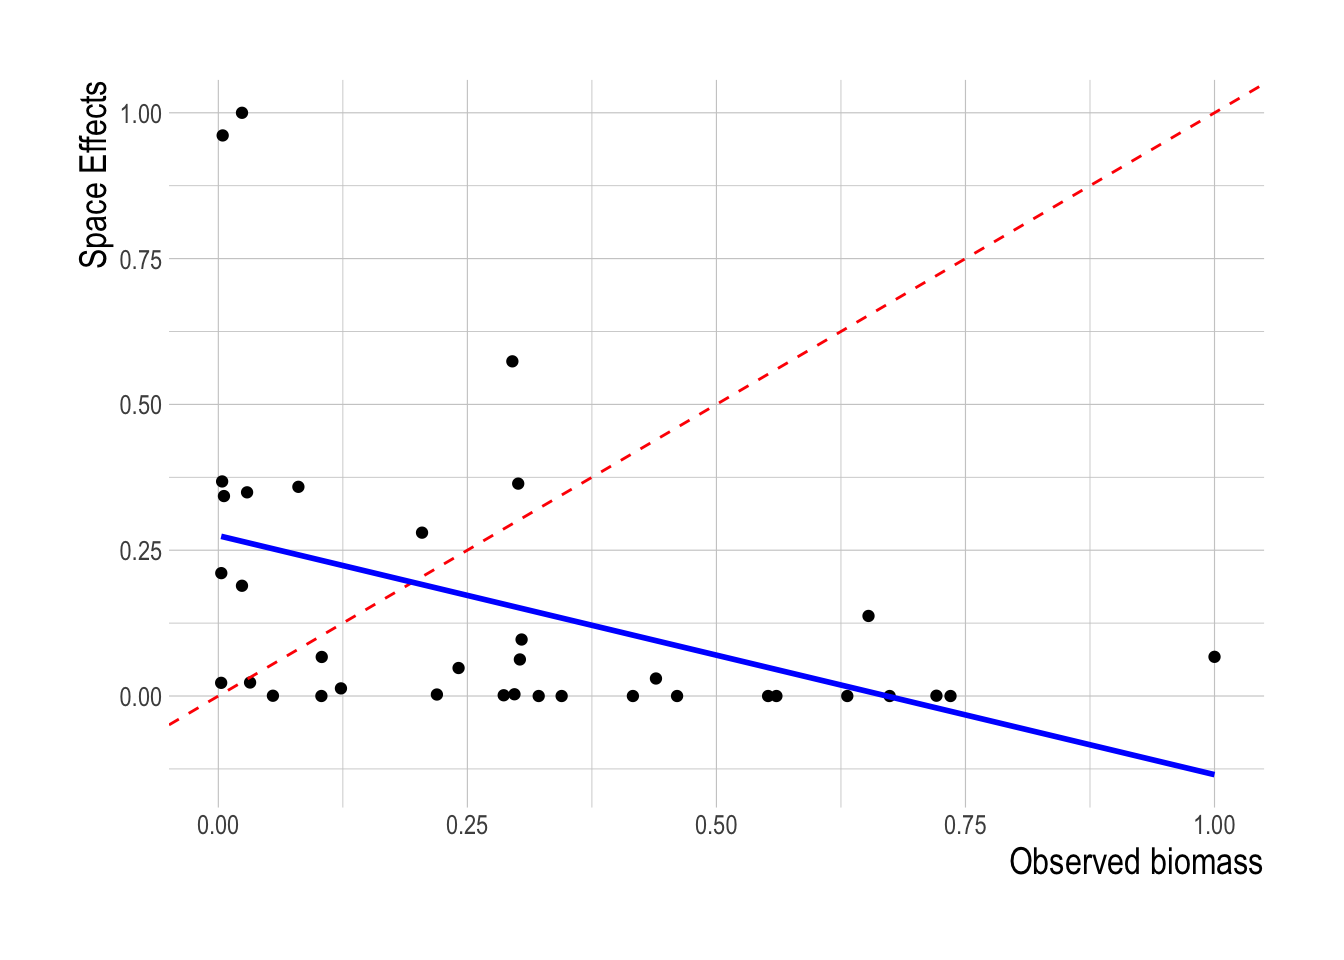
\includegraphics{thesis_files/figure-latex/strct-latent-plot-1.pdf}
\caption{\label{fig:strct-latent-plot}Scaled latent biomass coefficients
plotted against paired scaled biomass estimates. Red dashed line shows
1:1 relationship, blue line a fitted linear model to the observed and
predicted values}
\end{figure}
\subsection{Machine Learning Models}\label{machine-learning-models}

Linear and structural models demonstrate little ability to accurately
predicting fish abundance using effort data. We turned to machine
learning as a final strategy for predicting fish abundance using fishing
effort. We tested four different machine learning approaches: random
forests (ranger, Breiman \protect\hyperlink{ref-Breiman2001}{2001}),
gradient boosted machines (gbm), and multivariate adaptive regression
splines (bagged MARS and MARS models). Each of these machine learning
models is designed to make use of supplied data to maximize
out-of-sample predictive power. However, each model also contains a
number of tuning parameters that can only be reliably selected by
cross-validation. To that end, we used the \texttt{caret} package in R
(Kuhn \protect\hyperlink{ref-Kuhn2008}{2008}) to perform two repeats of
ten fold cross validation across factorial combinations of candidate
tuning parameters, and selected the set of tuning parameters that
minimized the out-of-sample root mean squared error (RMSE).

With those tuning parameters in hand, we then utilized the
cross-validation routines from those selected tuning parameters to
quantitatively compare each of the tuned machine learning models in
terms of their out-of-sample predictive power. For each model, we have
twenty out-of-sample RMSE estimates. We used the \texttt{tidyposterior}
package to fit a Bayesian hierarchical model that, controlling for split
effects, estimates the relative effect of each candidate model on
out-of-sample RMSE. Based on this analysis, the random forest model (as
implemented by the \texttt{ranger} package) has the lowest estimated
out-of-sample RMSE. As such, we use the random forest, as implemented by
the \texttt{ranger}, as our candidate machine learning model for the
remainder of this paper.
\begin{figure}
\centering
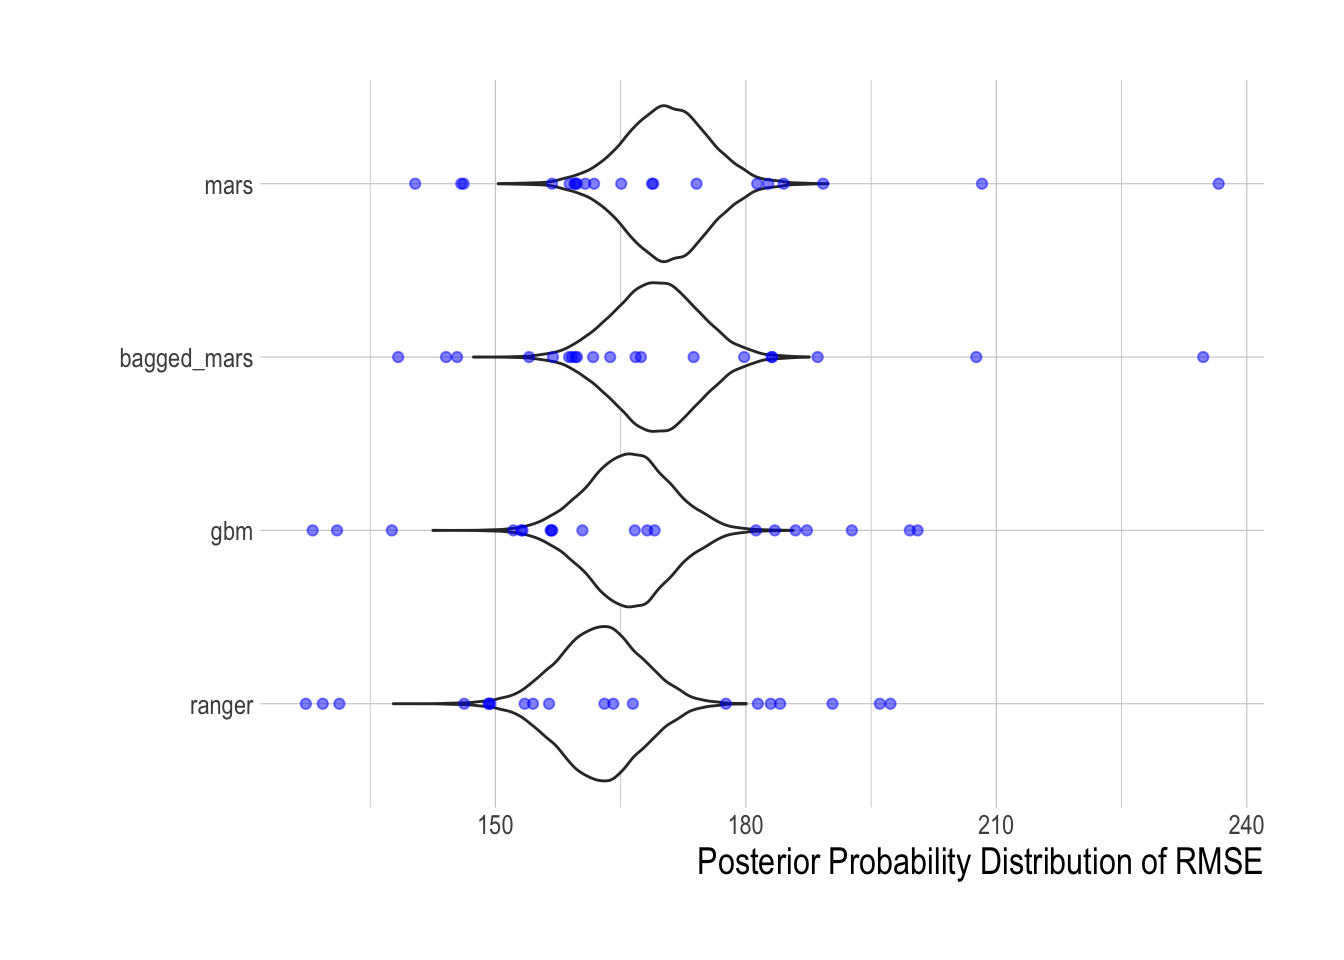
\includegraphics{thesis_files/figure-latex/best-ml-plot-1.pdf}
\caption{\label{fig:best-ml-plot}Posterior densities of out-of-sample RMSE
predicted by \texttt{tidyposterior}}
\end{figure}
The other decision to be made within the model fitting process is what
resolution of data to use within the fitting process. The finest scale
effort data pulled from Global Fishing Watch provides the largest sample
size, but also potentially increases the noise in the data. Aggregating
the data at coarser spatial aggregations decreases sample size but also
may decrease noise. We tested the models at three different spatial
resolutions, raw, at 25km\textsuperscript{2} resolution, and
100km\textsuperscript{2} resolution. The 100km\textsuperscript{2}
resolution had the highest R\textsuperscript{2} for the training data,
and so we will use that as our default resolution for this analysis
(Fig.\ref{fig:ml-res-plot}). Using the 100km\textsuperscript{2}
resolution data, the random forest has substantially greater predictive
ability within the training data split than any of the linear or
structural approaches, with a median R\textsuperscript{2} across the
training splits of over 0.5 (though the model also appears to be
positively biased, Fig.\ref{fig:ranger-ovp}).
\begin{figure}
\centering
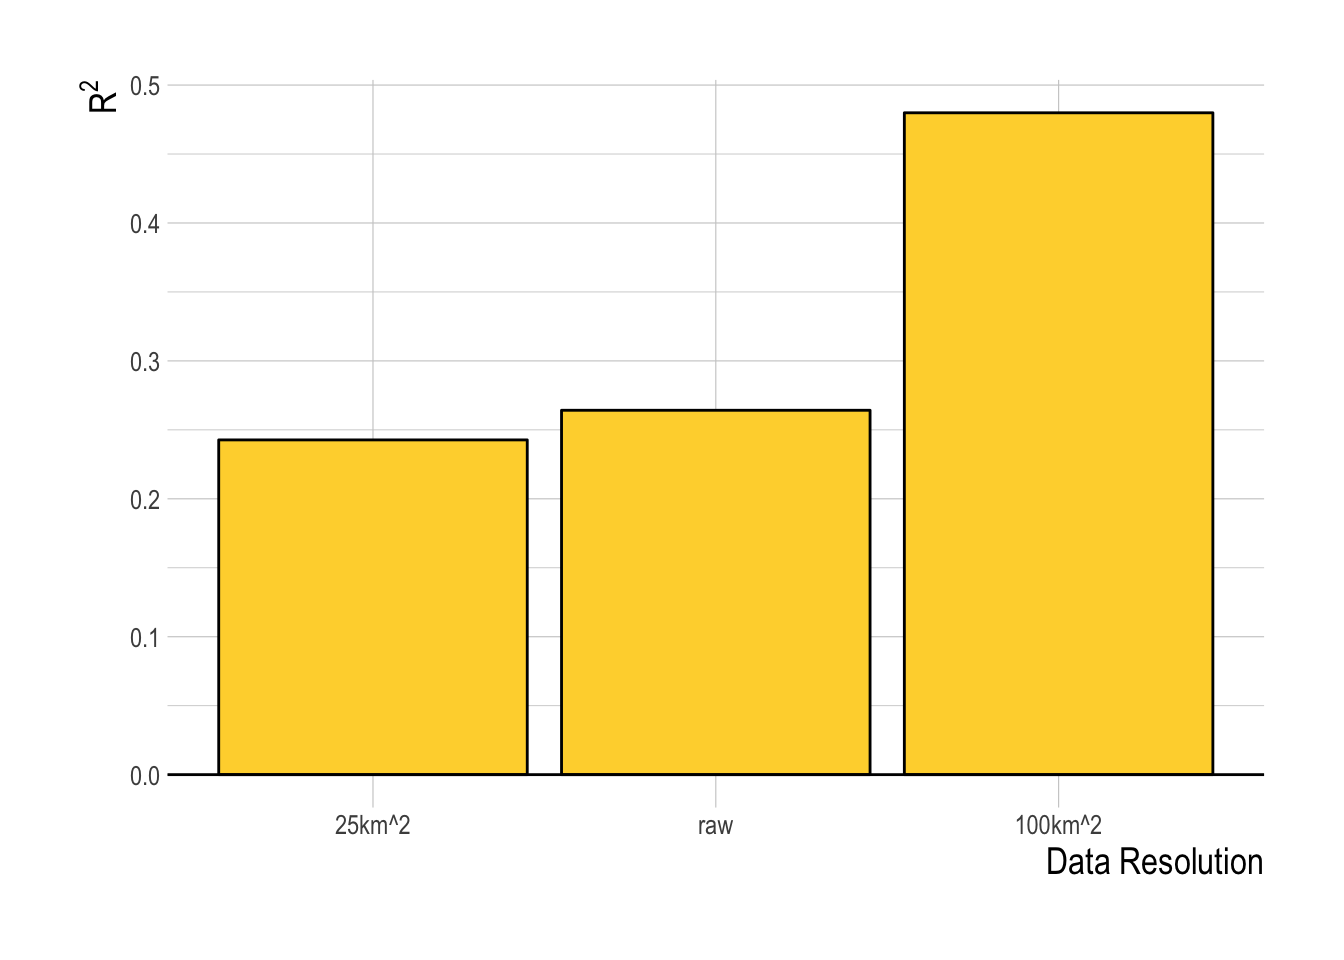
\includegraphics{thesis_files/figure-latex/ml-res-plot-1.pdf}
\caption{\label{fig:ml-res-plot}Training data R2 for the random forest
(ranger) model at three evaluated spatial resolutions of the data}
\end{figure}
\begin{figure}
\centering
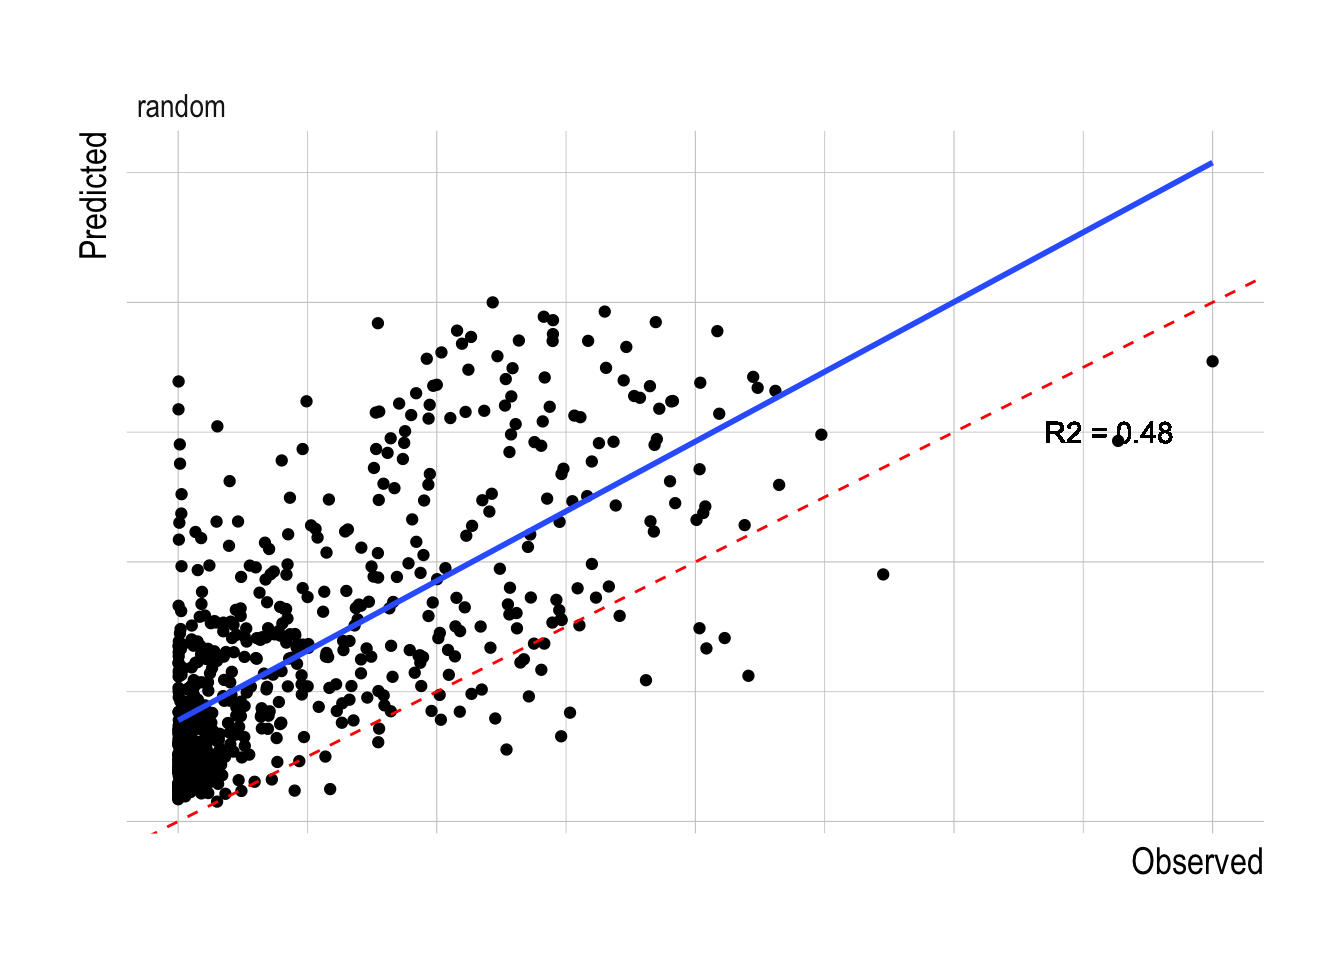
\includegraphics{thesis_files/figure-latex/ranger-ovp-1.pdf}
\caption{\label{fig:ranger-ovp}Observed vs predicted biomass for the fitted
random forest models across different evaluated data splits. Red dashed
lines indicates 1:1 fit, blue line a fitted linear model to the observed
and predicted values}
\end{figure}
We can repeat this same resolution procedure to perform one final
performance comparison between the random forest and structural models.
For each model, we fit the model using the finest resolution data, and
then aggregated predictions up to coarser resolutions
(Fig.\ref{fig:strct-v-ml-plot}-A), and refit the model itself using
coarser resolution data (Fig.\ref{fig:strct-v-ml-plot}-B). Using coarser
resolution data in the model fitting process improves the predictive
power of the structural models somewhat, but the random forest still
outperformed the structural approach across all spatial resolutions.
This analysis confirms that a spatial resolution of
100-200km\textsuperscript{2} appears to be ideal in terms of balancing
noise reduction with sample size.
\begin{figure}
\centering
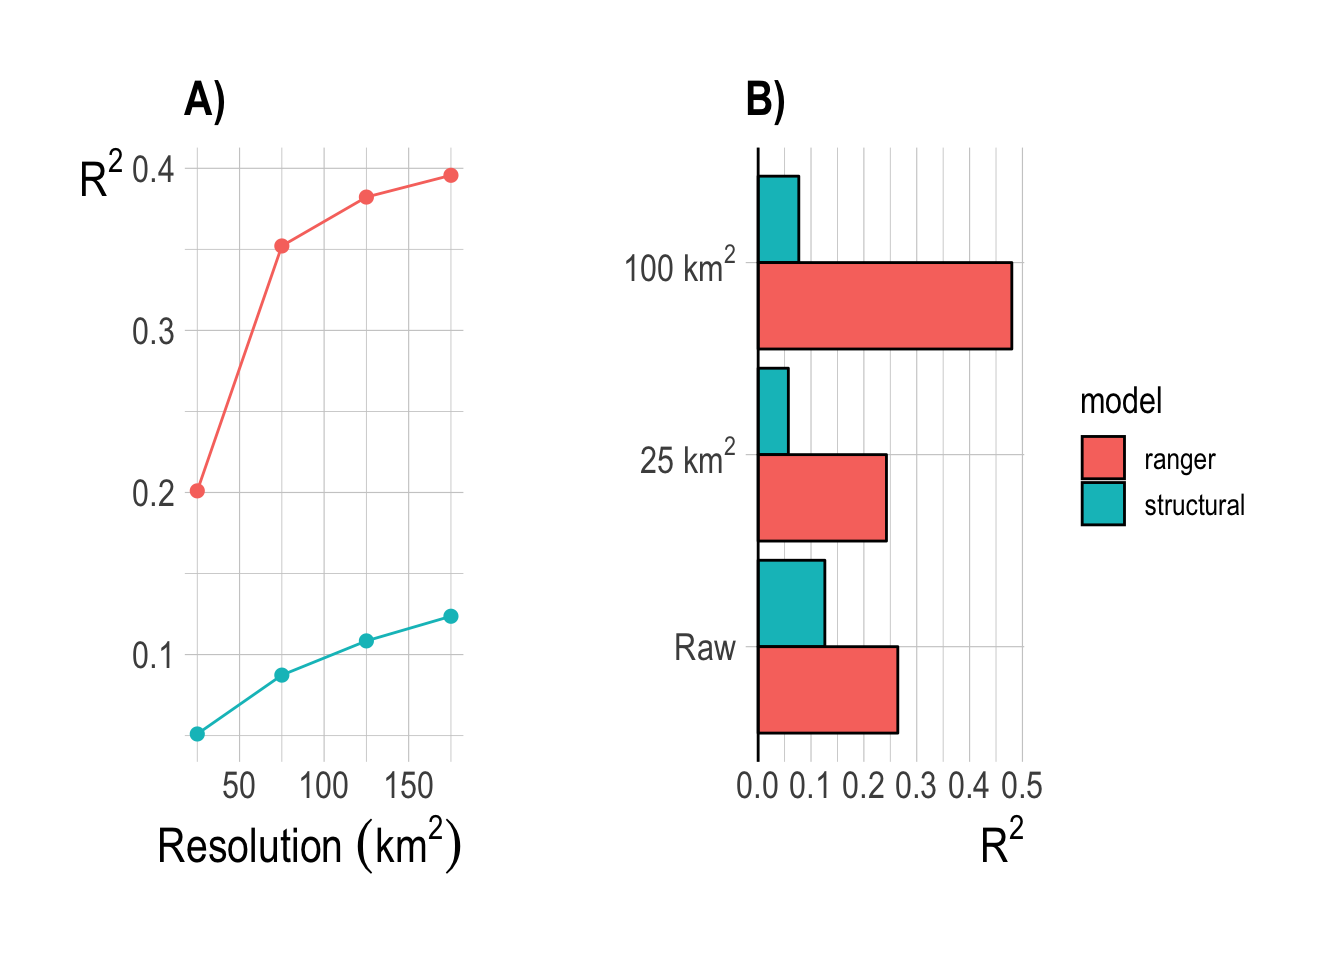
\includegraphics{thesis_files/figure-latex/strct-v-ml-plot-1.pdf}
\caption{\label{fig:strct-v-ml-plot}Training set R2 from aggregating results
of model fit on finest resolution (A) and fitting the model at coarser
resolutions (B)}
\end{figure}
\subsection{Value of Information}\label{value-of-information}

So far, the model with the greatest predictive power, as measured by the
R\textsuperscript{2} of the model within the training data, is a random
forest model trained on a random subset of the available data aggregated
at a 100km\textsuperscript{2} resolution. Under those conditions, we see
training set R\textsuperscript{2} in the vicinity of 0.5. Is this good?
Models such as Costello \emph{et al.}
(\protect\hyperlink{ref-Costello2012a}{2012}) report
R\textsuperscript{2} values near 0.4, so 0.5 would appear to be a
respectable value. However, the explicit purpose of this analysis is to
determine the value of the effort data supplied by Global Fishing Watch
for estimating fish biomass To get at this, we can compare the
predictive power of the Global Fishing Watch based model to an
alternative model for estimating fish abundance using different sources
of information. There are clear theoretical reasons to believe that
fishing effort should respond to and affect fish biomass. However, the
environment also plays a substantial role in driving fish dynamics, both
in abundance and spatio-temporal distribution (Szuwalski and Hollowed
\protect\hyperlink{ref-Szuwalski2016}{2016}; Munch \emph{et al.}
\protect\hyperlink{ref-Munch2018}{2018}). A model of fish abundance
based solely on environmental drivers makes at least as much conceptual
sense as a model based on effort and fleet characteristics then.

Based on this idea, we pulled globally estimates of chlorophyll
concentrations (a measure of primary productivity), along with sea
surface temperature, and bathymetry, from the National Oceanic and
Atmospheric Administration ERDDAP platform. We paired these data with
non-effort based data pulled from Global Fishing Watch (distance from
shore, MPA status), since these data are not part of the novel effort
data provided by Global Fishing Watch. We then refit the machine
learning models (since the structural models require effort data) using
only the environmental data, and using both the environmental data and
effort data (following identical fitting procedures across all runs).
This allows us to assess the change in predictive power (as measured by
R\textsuperscript{2} of the training data) that including effort data
provides.

Comparing effort data alone vs environmental data alone, we see that the
relative value of information of the effort data is in fact negative.
Meaning, the environment-alone model substantially outperformed, in
terms of training data R\textsuperscript{2}, the effort-alone model. If
the effort data by themselves are not as predicatively useful as
environmental drivers, are the effort and environmental data together
worth more than the sum of their parts? Our results suggest that in fact
they are not; combining the effort data with the environmental data
provides nearly identical performance to using just the environmental
data (Fig.\ref{fig:voi-plot}).
\begin{figure}
\centering
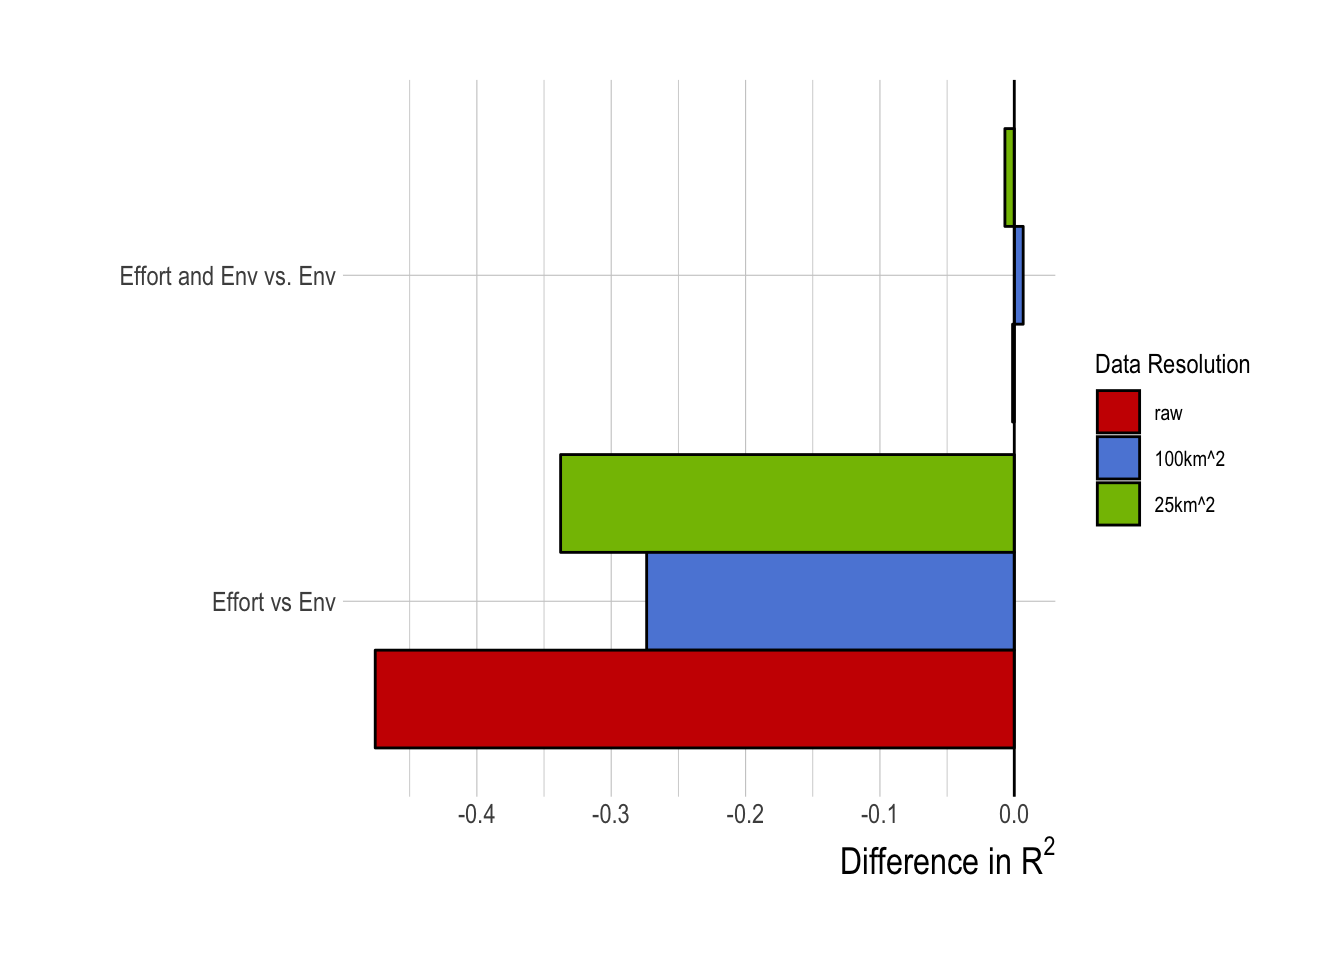
\includegraphics{thesis_files/figure-latex/voi-plot-1.pdf}
\caption{\label{fig:voi-plot}Differences in R2 of tuned random forest model
with effort data relative to R2 obtained from only using environmental
(env) data (negative implies worse performance than environmental data
only)}
\end{figure}
\subsection{Confrontation with Testing
Data}\label{confrontation-with-testing-data}

The preceding steps have determined that the best model, in terms of
training data R\textsuperscript{2}, is a random forest fitted with data
aggregated at the 100km\textsuperscript{2} resolution, using both
environmental and effort data. The end goal of this model though is not
to predict data within the training set; instead, we would hope to use
this model to help us understand fish abundance in situations outside of
the data used to train the model, either in space (i.e.~new locations)
or time (periods not covered by the trawl surveys). As discussed
earlier, the decision of what model to use must be made by examining the
training data (and splits of the training data) alone. Now that we have
used the training data to select a model that the evidence suggests will
have the highest chance of performing well out of sample (remember that
even within the training data, the random forest looks to avoid
overfitting), we can now confront our selected model with the held out
testing data. We also include the structural models in this comparison
to see if the structural assumptions of these models provide an
advantage in out-of-sample prediction, though we have not provided the
structural model with the same built-in resistance to overfitting to the
training data that the machine learning models benefit from.

The predictive performance of our candidate models against the testing
data indicate that the decisions based on the training data were well
founded. Inclusion of the effort data did not improve the performance of
the models on the testing data, and across nearly all cases the machine
learning approaches still outperformed the structural models. Looking at
just the random test-training splits then, our results would seem to
show that a random forest based largely on environmental drivers is a
good out-of-sample predictor of fish abundance. Before we start
replacing stock assessments with remote sensing of environmental drivers
though, we should look at the out-of-sample performance of the models
trained on other data splits (Fig.\ref{fig:test-training-plot}).

Under the ``historic'' data split, the training split consists of
observations from 2012-2013 and the testing split from 2014-2017. Under
this split the performance from the training to the testing split drops
off much more dramatically than under the random split, showing that
predicting new years is a much more challenging task for the model than
filling in gaps within a year. Similarly, we see that a model trained on
data off of the Washington/Oregon coast alone is almost completely
useless as a predictor of fish biomass off of California.
\begin{figure}
\centering
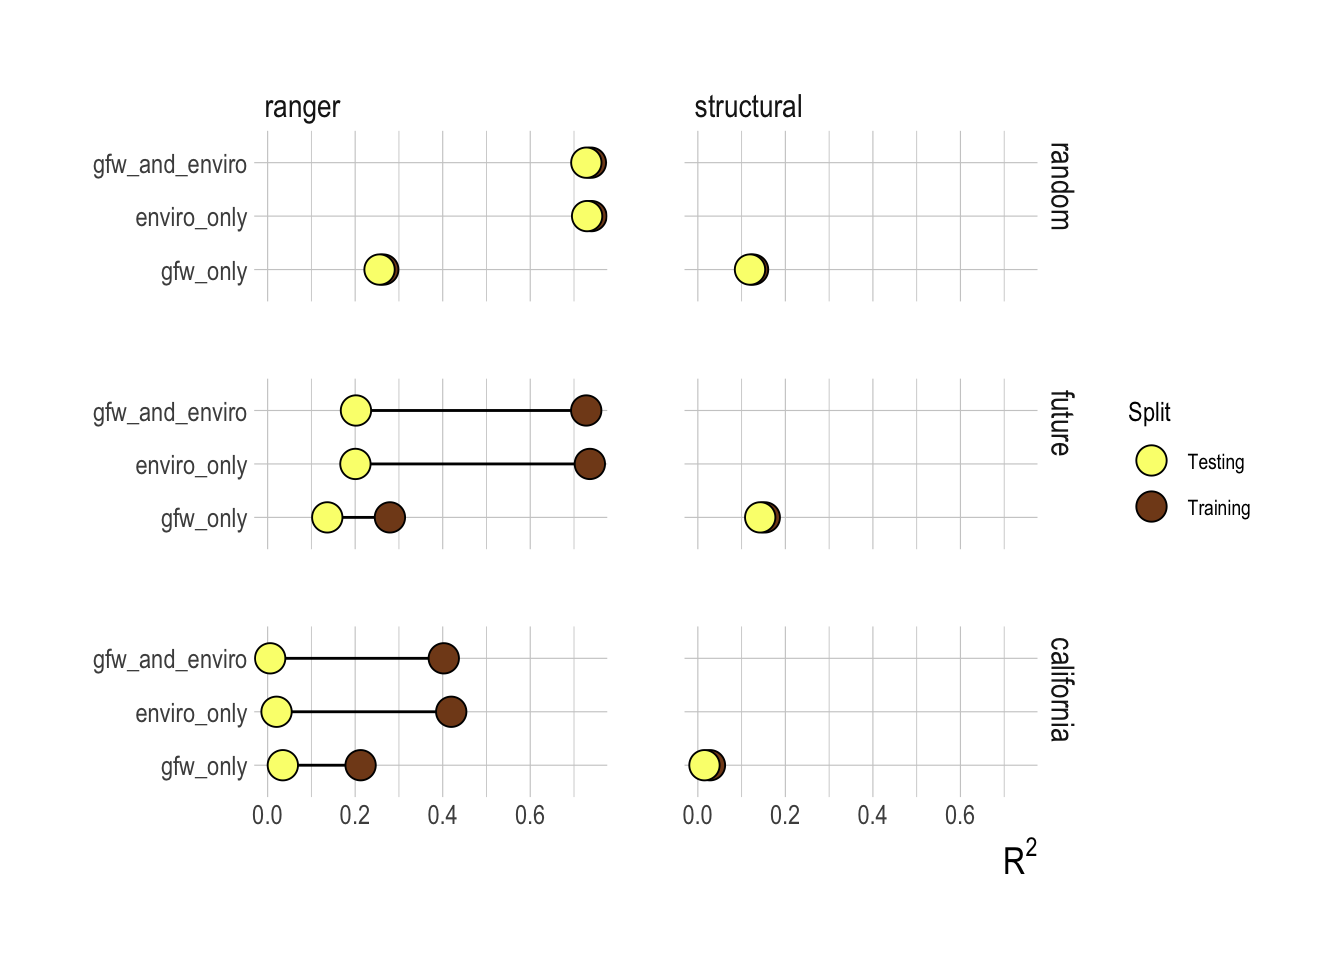
\includegraphics{thesis_files/figure-latex/test-training-plot-1.pdf}
\caption{\label{fig:test-training-plot}R2 for testing and training splits
across candidate variables and models. Columns represent the ranger
(random forest) and structural models, rows are test-training splits,
where row name indicates the dataset that was held out for testing}
\end{figure}
Our analyses so far have focused on R\textsuperscript{2} values as a
measure of predictive accuracy. These R\textsuperscript{2} values
represent the fraction of the variation in spatio-temporal fish
abundance explained by each of our models. A model with an
R\textsuperscript{2} of say 0.9 would then likely be very good at both
replicating both a map of abundance and a plot of abundance over time
(made up of aggregating each of the individual location estimates over
time). However, it is entirely possible that a model with a poor
predictive R\textsuperscript{2}, while unlikely to do a good job of
capturing the spatial distribution of abundance, may still provide a
reasonable index of the trend in abundance (if each point is off but all
on average reflect a common trend).

To explore this idea, we can examine the ``future'' testing case more
carefully. In this data split, we trained all models on data from
2012-2013, and used the fitted coefficients from this period to predict
data from 2014-onward. Using this model, we then summed the total
biomass predictions across space to create a total estimate of biomass
within a survey region and a given year. Examining the results, we see
that all of the models show evidence of capturing aspects of the trend
in the 2014-onward period. In the Eastern Bering Sea region in fact, the
random forest model using only Global Fishing Watch data appears to do a
slightly better job of representing the trend in the observed abundance
trends, though with only four data points it is not wise to make any
definitive statements about this, especially since this pattern is
reversed in the West Coast data, where use of the environmental data
provides better projected predictions (Fig.\ref{fig:future-fit}).
\begin{figure}
\centering
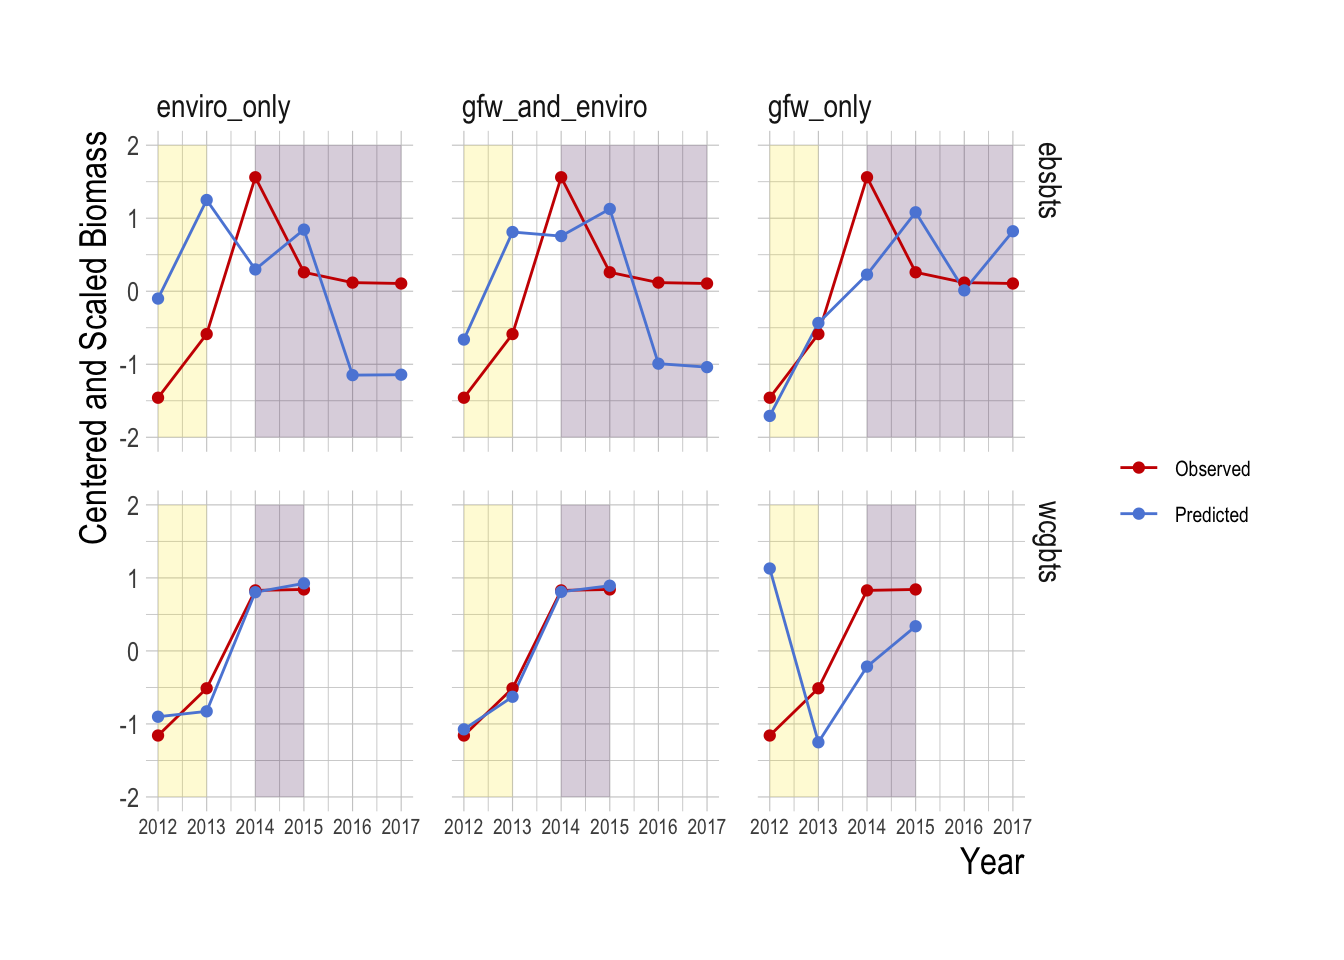
\includegraphics{thesis_files/figure-latex/future-fit-1.pdf}
\caption{\label{fig:future-fit}Observed (red) and predicted (blue) centered
and scaled total biomass estiamtes over time. Yellow regions indicate
data used in the training model, purple shaded regions data held out
from the model training. Note that in order to avoid problems with
increasing spatial coverage in the GFW data, only locations consistently
present over the entire timespan of the data are included}
\end{figure}
\section{Discussion}\label{discussion}

The goal of this project was to determine the value of the effort data
provided by Global Fishing Watch in estimating fish abundance in space
and time. We accomplished this by first determining through a set of
fitting routines (models, tuning parameters, resolution) the model that,
given the training data, appeared to provide the highest likelihood of
performing well, in terms of predictive ability, both in and out of
sample. This process found a random forest tuned on
100km\textsuperscript{2} spatial resolution data to be the ``best''
model. From there, we were able to estimate the value of information of
the effort data by comparing the predictive power of the selected model
using effort data, as compared to the same selected model using only
non-effort based data. This analysis showed that the effort data
provides little predictive power beyond that provided by the non-effort
data alone.

That the machine learning models outperformed the liner and structural
models comes as no surprise: machine learning models are designed
explicitly for prediction and should be expected to do well at the task.
However, they have two central weaknesses that made the evaluation of
alternative predictive models important. The first is that they lack any
structural assumptions, and therefore are relatively un-interpretable.
Structural models, such as the bio-economic approach taken here, require
assumptions about specific functional forms, but as a result provide a
means for rationalizing results, e.g.~by providing parameter estimates
that can be evaluated and interpreted using statistical methods and
theoretical knowledge (e.g.~the meaning of a cost coefficient can be
understood and our confidence in the value of that coefficient
estimated). All else being equal, we would clearly prefer to have an
interpretable model than a black box. To that end, when prediction is
the objective, we can estimate the ``cost'' of that interpretability by
comparing the predictive ability of a machine learning approach that
maximizes predictability of at the expense of interpretability to a
structural model that seeks to maximize the likelihood of the data
conditional on its assumptions. While, during the training phase, the
structural model is unlikely to outperform the machine learning
approach, if it comes close, the price in predictability may be well
worth the gain in interpretation. In our case though, the machine
learning approach so outperformed the structural approach that they
cannot be outweighed by the interpretability of the structural approach.
This does not mean that the broad concept of the ideal-free distribution
that is at the core of the structural model is inherently incorrect, but
that that particular model as implemented here is not suitable for the
aggregation of the data as they stand. It is entirely possible that
finer resolution effort and abundance data (e.g.~the logbook data
utilized in Miller and Deacon
(\protect\hyperlink{ref-Miller2016}{2016})) would produce better
performance from the structural model. But, our results show that a
structural bio-economic modeling approach is not appropriate for using
the effort data supplied by Global Fishing Watch to estimate fish
abundance.

Vastly out-of-sample prediction is a second major problem with machine
learning models, and the random forest model selected through this
process in particular. A properly specified and estimated structural
model provides a clear process for predicting outcomes in situations
that are far outside of the scale of the training data. Suppose for
example that the structural model is a simple linear regression with a
slope and intercept, trained on one independent variable on the range
one to twenty. If we then confront our fitted model with a new
independent datapoint with value of 1,000, our estimated slope and
intercept allows us to easily provide a prediction for this new data
point (though of course the accuracy of this prediction will depend on
the accuracy of our model). A random forest is able to do this process
as well, but lacks a clear mechanism for doing so. A random forest works
by fitting a forest of regression trees, each of which, in the case of
continuous predictors, break the predictors into a series of bins.
Therefore, the predicted outcome for a dependent variable 100 times
greater than any value used in the training value will be more or less
the same as the prediction for the largest value of the dependent value
in the training data (i.e.~the new data point will fall into the
``greater than some cutoff'' bin). If there is some continuous
relationship between the dependent variable and the outcome, this
prediction may be severely biased. Because of that, machine learning
models such as random forests are best at ``filling in the gaps'' for
data fitting within a defined parameter space, and can struggle when fit
on one parameter space and applied to a vastly different parameter
space.

We checked for the possibility of this problem by, post selection of the
random forest model, examining the predictive ability of that model on
both the testing data and the held out training data. Our results show
that this flaw of random forests is indeed a problem here: the model
does very well at predicting ``out of sample'' points that are simply
random omissions from the complete database. A model trained on the
years 2012-2014 and used to predict 2015-2017 (the ``future''
training-test split) performs worse than the random split, and a model
trained on Washington/Oregon data and used to predict California losses
roughly half of its predictive power. However, the structural model was
still not able to outperform the machine learning approach in these
out-of-sample cases. These results show that there are predictable
relationships between fish biomass and environmental, and to a lesser
extent effort, data, but that these relationships do not easily export
to new time periods or locations.

What should we make of the relative lack of predictive value of the
effort data, as compared to the environmental data? It is critical to
note that this is not to say that the effort data alone does not have
predictive power, at least within the rough survey region and time
period on which the models are trained. R\textsuperscript{2} values for
a random forest using only GFW data trained on a random subset of the
data to predict fish biomass were near 0.5, both for the training and
testing splits; the effort data alone are capable predictors. But, if
the question is what additional predictive power do these effort data
provide us that we could not have obtained from other data streams, such
as environmental data, the answer is not much. We do see closer
performance of the effort based and environment based models when
comparing their ability to predict trends in abundance, as opposed to
overall fit (Fig.\ref{fig:future-fit}). This may suggest that effort
data supplied by GFW may be more indicative of overall trends in
abundance than the exact spatial distribution of abundance However,
given the very short time-span over which both effort and abundance data
are available, we cannot draw definitive conclusions about the ability
of these models to predict trends at this time.

While the effort data's lack of value in predicting fish is not the
result that we hoped for, it is not surprising for two reasons. The
first is that this is simply an indication of the long-understood
challenges of using effort data alone to make meaningful inferences on
the status of fish stocks: more fishing might mean abundant fishing
grounds or over-exploited locations where the fishing is cheap. While
machine learning approaches may be able to disentangle some of these
factors within a region, a relationship between fishing and effort
fitted in one region is unlikely to export to a new region or time. A
second and more interesting reason though may lie in the nature of the
information used by fishermen to make their decisions. While many
bio-economic modeling exercises assume perfect knowledge of the location
and amount of fish stocks for simplifying reasons, in reality of course
the choice of where and how much to fish is an uncertain and complicated
process, based on objectives, risk tolerance, past experience and shared
knowledge. Part of that decision making process is directly related to
observing and reacting to the precise type of environmental drivers
included in this analysis. Fishermen understand the preferred depth and
temperature contours of their target species, and areas of substantial
upwelling, often marked by increased chlorophyll concentrations, have
long been known to be productive fishing grounds. So, while the model
hypothesized that combinations of environmental and effort data might
provide a signal worth more than the sum of their parts, our results
suggest in fact with regards to predicting biomass, the effort data are
a noisier reflection of the environmental data, but further muddied by
the myriad other factors affecting fishing decisions, including costs,
regulations, experience, and safety.

The effort data provided by Global Fishing Watch present a novel and
massive influx of information that shed light on a variety of different
factor affecting our oceans, including the footprint of global fishing
(Kroodsma \emph{et al.} \protect\hyperlink{ref-Kroodsma2018}{2018}) to
the estimates of the profitability of different fishing regions (Sala
\emph{et al.} \protect\hyperlink{ref-Sala2018}{2018}). This project
evaluated the extent to which these data could be used to improve
fisheries management by helping estimate fish abundances associated with
different effort patterns. We found that these effort data can be used
for predicting fish biomass, but that a) the manner in which effort is
related to abundance, at least at these aggregated resolutions of
multiple gears and multiple species, is poorly described by classical
bio-economic models, and that b) while machine learning models were able
to provide much greater predictive power, the effort data provided
little additional predictive value over other globally available
environmental datasets. Further work utilizing effort data derived from
Global Fishing Watch in stock assessment will need to find ways of more
closely matching effort data with their targeted species, or shift
attention from using effort as an indicator of biomass towards using it
as a prior on the evolution of fishing mortality rates.

\chapter{Predicting and Detecting the Regional-Scale Conservation and
Fishery Impacts of Marine Protected Areas}\label{zissou}

\section{Introduction}\label{introduction-2}

Marine Protected Areas (MPAs, which we will define here as spatial
regions in the ocean in which fishing for species of interest is
prohibited, acknowledging that other regulatory definitions of MPAs
exist) have a long history in the management of marine resources.
Traditional cultures in Oceania utilized (often temporary) MPAs as a
sort of ``fish bank'' for times of need (Johannes
\protect\hyperlink{ref-Johannes1978}{1978}). In more recent times, MPAs
were first put in place primarily as conservation areas, analogs to
terrestrial reserves deigned to protect iconic landscapes such as
Yellowstone or Kruger National Parks. However, over time our goals and
expectations for MPAs have evolved; we now frequently consider the use
of MPAs to both protect marine ecosystems within their boundaries and
bolster fish populations and fishing opportunities in their surrounding
waters (Gaines \emph{et al.} \protect\hyperlink{ref-Gaines2010}{2010}).

We have clear and compelling evidence that well enforced MPAs can
provide conservation benefits within their borders (Halpern and Warner
\protect\hyperlink{ref-Halpern2003}{2003}; Lester \emph{et al.}
\protect\hyperlink{ref-Lester2009}{2009}; Edgar \emph{et al.}
\protect\hyperlink{ref-Edgar2014}{2014}). As conservation benefits
accrue inside an MPA, the MPA can affect the waters beyond their borders
through adult or larval spillover, meaning the export of either adult or
larval fish from within an MPA's borders to surrounding waters. Several
studies have documented empirical evidence for the existence of adult or
larval spillover affecting both abundance and fisheries (Russ and Alcala
\protect\hyperlink{ref-Russ1996}{1996}; McClanahan and Mangi
\protect\hyperlink{ref-McClanahan2000}{2000}; Stobart \emph{et al.}
\protect\hyperlink{ref-Stobart2009}{2009}; Halpern \emph{et al.}
\protect\hyperlink{ref-Halpern2009}{2009}; e.g. Goni \emph{et al.}
\protect\hyperlink{ref-Goni2010}{2010}; Kay \emph{et al.}
\protect\hyperlink{ref-Kay2012}{2012}; Thompson \emph{et al.}
\protect\hyperlink{ref-Thompson2017}{2017}). Given the lack of attention
paid by most fish and their larvae to lines on a map, there is no doubt
that some degree of spillover occurs from MPAs. The more complex
question then is not whether spillover occurs, but what the net effect
of spillover is. From a fishery perspective, are spillover benefits
sufficient to offset losses in fishing grounds? From a conservation
perspective, how much does the buildup of adults inside an MPA increase
abundance outside, or does concentration of fishing outside the reserve
result in a net loss in regional abundance?

As stakeholders around the world increasingly seek to use MPAs in the
marine resource management portfolios, it is critically important that
we develop a better understanding of the magnitude and drivers of
regional-scale MPA effects. To address this gap, this study examines two
critical questions: 1) What do we expect the regional-scale conservation
effects of MPAs to be and 2) When (and how) can we expect to detect
these effects? We address these questions using a simulation analysis
framework to frame the theoretical regional conservation and fishery
impacts of MPAs, from which we then develop an empirical assessment of
the evidence for regional-level effects of MPAs resulting from a network
of closures put in place in the Channel Islands, California, in 2003.

\subsection{What Does Theory Tell Us?}\label{what-does-theory-tell-us}

Before we start, we should define ``regional-scale MPA effects'' for the
purposes of this paper. We define regional-scale conservation MPA
effects as the change in total biomass of fish (summing inside and
outside of MPAs) relative to the total biomass fish that would have
occurred without the MPA In clearer words, how many more or less fish
are there throughout the study region as a result of one or more MPAs?
Note that this is different from questions such as do MPAs cause an
increase of fish inside their borders, or do connected networks of MPAs
provide greater benefits than isolated MPAs with equal coverage
({\textbf{???}}). From the fisheries perspective, we define regional MPA
effects as the difference in fishery catches following implementation of
an MPA, relative to what the fishery would have caught in the absence of
the MPA. Defining ``regional'' is not a clear-cut exercise. Regional
could be defined as a bio-geographic area (e.g.~the Channel Islands), or
as the range of a interbreeding population (in line with a fisheries
definition of a ``stock''), or through the range of connectivity of a
species through movement. For brevity's sake, for the remainder of this
paper we will refer to the ``regional-scale conservation MPA effects''
as conservation effects. While the definition of an appropriate region
will vary from place to place, the key point here is that we are
considering the net effect of MPAs both within and outside of their
borders, within a spatial area on which they are capable of having an
impact (see Fig.\ref{fig:ex-mpa} for an illustration of the regional
conservation MPA effect). For the empirical portion of this study, we
define ``regional'' as encompassing the central islands of the Channel
Islands National Marine Sanctuary: Anacapa, Santa Cruz, Santa Rosa, and
San Miguel.
\begin{figure}
\centering
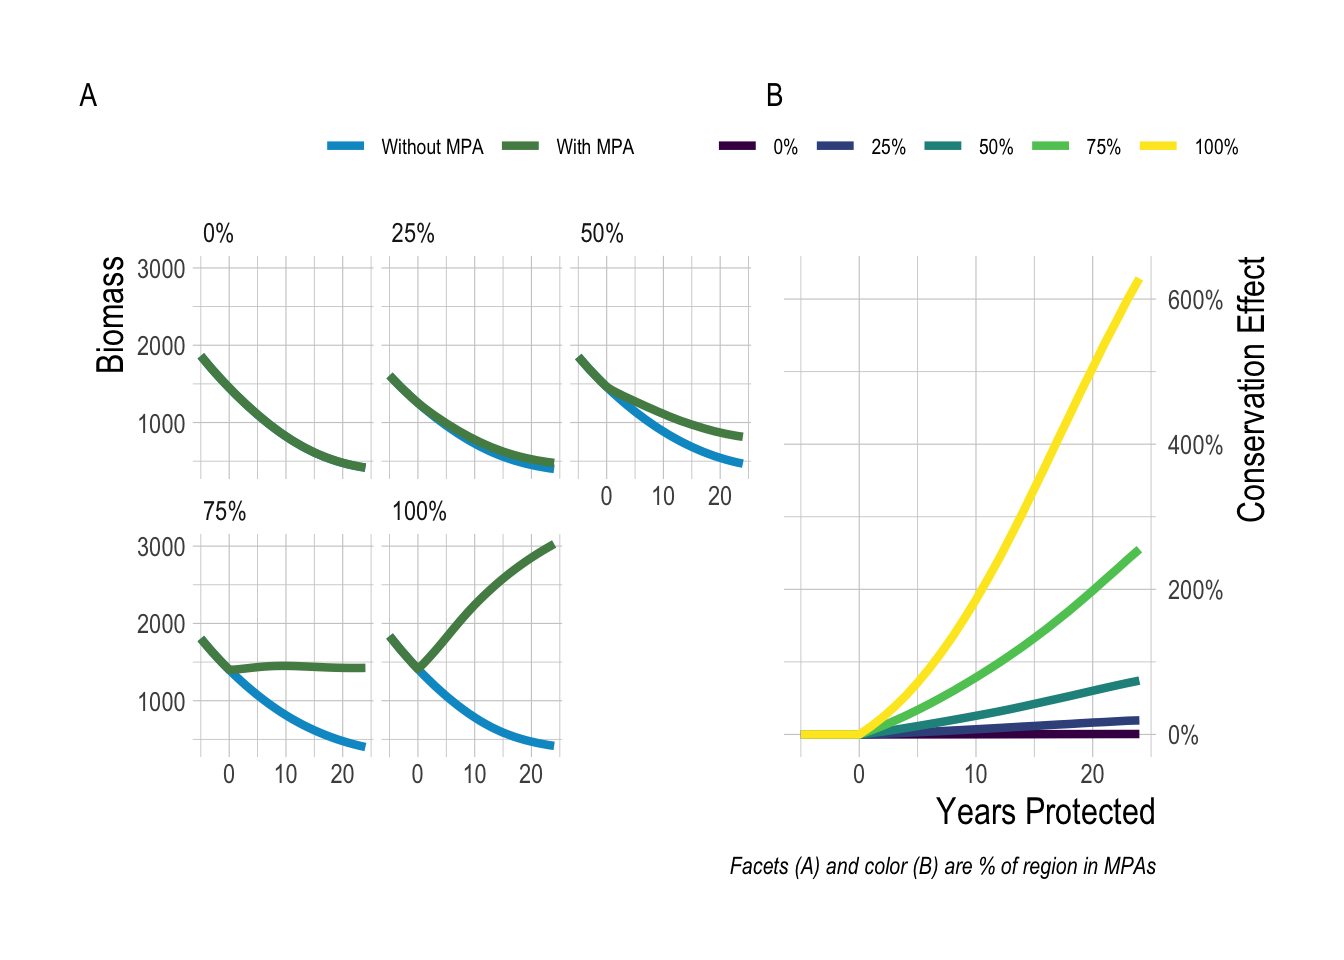
\includegraphics{thesis_files/figure-latex/ex-mpa-1.pdf}
\caption{\label{fig:ex-mpa}Example trajectories of biomass with and without
MPAs under a range of MPA sizes (A), and resulting MPA effect (B)}
\end{figure}
With that definition in mind, what does basic theory suggest should be
the magnitude of these regional effects? On one hand, if we imagine a
region that has driven its fish populations to near extinction that then
places 100\% of its waters inside a no-take MPA, we would expect the
regional-scale conservation effects to be massive, and in fact to
approach infinity (in terms of percentage increase) the closer the ``pre
MPA'' populations approach zero (assuming that the populations are not
so depleted as to prevent recovery). On the other hand, If we implement
an MPA in place for a lightly fished sedentary species, and in doing so
displace a large amount of fishing effort to the waters outside the MPA,
it is actually possible to create a net conservation loss. So, this
exercise tells us that regardless of almost any other factor, the range
of possible regional effects (on a percentage scale) spans the range of
of some negative number to positive infinity.

However, within these extremely broad bounds, numerous other factors can
act to affect the regional effects of MPAs. These include, but are
certainly not limited to, the scale of adult and larval dispersal
relative to the size of the MPAs ({\textbf{???}}; Gaines \emph{et al.}
\protect\hyperlink{ref-Gaines2003}{2003}; Botsford \emph{et al.}
\protect\hyperlink{ref-Botsford2008}{2008}), the strength and timing of
density dependence in the population (e.g.~pre or post settlement), how
overfished the population was pre-MPA, and how fishing activity responds
to the implementation of the MPAs (Hilborn and Walters
\protect\hyperlink{ref-Hilborn1992}{1992}; Gerber \emph{et al.}
\protect\hyperlink{ref-Gerber2003}{2003},
\protect\hyperlink{ref-Gerber2005}{2005}; Hastings and Botsford
\protect\hyperlink{ref-Hastings2003}{2003}; Hilborn \emph{et al.}
\protect\hyperlink{ref-Hilborn2004a}{2004}\protect\hyperlink{ref-Hilborn2004a}{a},\protect\hyperlink{ref-Hilborn2004}{b};
Walters and Martell \protect\hyperlink{ref-Walters2004}{2004}; Gaines
\emph{et al.} \protect\hyperlink{ref-Gaines2010}{2010}). In addition,
even for the same total area of MPAs, the location and spacing of the
MPAs can have a profound influence on their cumulative impact through
habitat and network effects (Costello \emph{et al.}
\protect\hyperlink{ref-Costello2010}{2010}; Gaines \emph{et al.}
\protect\hyperlink{ref-Gaines2010}{2010}). Broadly, a wide range of
theory and modeling exercises indicate that the expected effects of MPAs
can vary widely and are extremely context- dependent (Fulton \emph{et
al.} \protect\hyperlink{ref-Fulton2015}{2015}).

At the most ``conservation friendly'' side of things, we could imagine a
group of heavily fished species with limited home ranges as adults,
broadcast larvae throughout the region, have post-settlement density
dependence, and have a fishing fleet that exits the fishery in
proportion to the area protected inside MPAs (e.g.~a grouper fishery in
which fishing was dependent on a large spawning aggregation). Under
these circumstances, the MPAs can be expected to provide a substantial
influx of new recruits to the overfished areas outside of the reserve,
even as the reserve fills in with adults. At the other end, consider a
complex of lightly fished species with relative high adult mobility,
pre-settlement density dependence (e.g.~at the spawning level, for
example a species with specific space and habitat requirements for
breeding), and a fishing fleet that concentrates into the remaining
fished areas. Under these circumstances, it will be much more
challenging for the MPA to provide substantial conservation benefits.
Theory then helps us think about the likely regional effects of a given
MPA, but outside of these simple cases the cumulative effect of
interacting drivers means that the expected regional effects are not
analytically solvable or obviously predictable.

\subsection{What Empirical Evidence Do We
Have?}\label{what-empirical-evidence-do-we-have}

We focus here on evidence of effects of MPAs beyond their borders, see
Lester \emph{et al.} (\protect\hyperlink{ref-Lester2009}{2009}) for a
thorough review of within-MPA effects. Many of the studies that explore
the effects of MPAs outside of their borders focus on studying gradients
of abundance, commonly measured through catch-per-unit-effort (CPUE) or
estimated densities along a distance gradient from MPA borders. Presence
of negative gradients (decreasing CPUE with distance from MPA border) is
taken as evidence of ``spillover'', or the export of (generally) biomass
from MPAs to their surrounding fished areas

Halpern \emph{et al.} (\protect\hyperlink{ref-Halpern2009}{2009})
conducted a rigorous meta-analysis of empirical evidence for spillover
from MPAs. They find that frequent evidence for spillover from MPAs, but
at relatively small spatial scales (on average up to 800m from reserve
boundaries), though since these studies are in fished system, it is
unclear if this distance is reflective of the biological range of
spillover, or the intensity of fishing pressure along the border of an
MPA. Gell and Roberts (\protect\hyperlink{ref-Gell2003}{2003}) surveyed
empirical evidence for adult and larval spillover from MPAs. They
documented numerous examples of studies showing decreases in CPUE of
adult biomass with distance from MPA borders, commonly attributed to
buildup of density inside MPAs and subsequent export of fish biomass,
though they also note that evidence for larval spillover is less
reported, likely since it is much more difficult to measure than adult
biomass (as opposed to an alternative explanation which is that larval
spillover happens less than adult spillover).

Russ and Alcala (\protect\hyperlink{ref-Russ1996}{1996}) documents
changes in densities or large predatory fish inside and outside of a
small marine reserve on Apo Island, Philippines (0.45km long at the
time). They report a positive correlation between years of MPA existence
and fish densities, but note that up to 8 years of protections were
required to detect a significant gradient in fish densities radiating
from the reserve borders. Russ \emph{et al.}
(\protect\hyperlink{ref-Russ2003a}{2003}) presents a similar study
focused on the surgeonfish \emph{Naso vlamingii}, in which they find
dramatic density increases within the reserve, as well as a strong
correlational relationship showing catch-per-unit effort of \emph{Naso
vlamingii} decreasing with distance from the reserve boundary.

Similarly, Harmelin-Vivien \emph{et al.}
(\protect\hyperlink{ref-Harmelin-Vivien2008}{2008}) assessed gradients
in fish density at increasing distances from cores of MPAs as evidence
of spillover in the Mediterranean. They report evidence of decreases in
biomass densities with distance from MPA borders, though these effects
largely dissipated within 100s of meters of MPA boundaries. Vandeperre
\emph{et al.} (\protect\hyperlink{ref-Vandeperre2011}{2011}) conducted a
meta-analysis of spillover effects (again measured as CPUE along
distance-from-MPA gradients over time) around MPA in Southern Europe.
They also document some evidence of declines in CPUE with distance from
MPA border, as well as a 2-4\% increase in CPUE per year in the fished
area following MPA implementation. Guidetti and Sala
(\protect\hyperlink{ref-Guidetti2007a}{2007}) finds similar results in
the region.

McClanahan and Mangi (\protect\hyperlink{ref-McClanahan2000}{2000})
measured spillover effects around the Mombasa Marine Park in Kenya. They
also provide evidence of negative CPUE gradients with distance from MPA
border, but note that these effects are highly affected by habitat,
environmental, and management variables. They document the largest
effects for moderately mobile species (e.g.~surgeonfish)

Several studies have explored the spillover effects of MPAs along the
California coast. Starr \emph{et al.}
(\protect\hyperlink{ref-Starr2015}{2015}) and Caselle \emph{et al.}
(\protect\hyperlink{ref-Caselle2015}{2015}) both document rapid but
variable changes in fish densities related to marine reserve networks in
the Channel Islands and along the central California coast. Starr
\emph{et al.} (\protect\hyperlink{ref-Starr2015}{2015}) found evidence
that densities inside MPAs had increased on average, but effects were
variable, and found little substantial changes in densities in control
sites outside the reserves. Caselle \emph{et al.}
(\protect\hyperlink{ref-Caselle2015}{2015}) found similar results,
documenting faster increases of densities of targeted species inside
reserves than outside, but little change in densities in reference
sites. Both of these studies then suggest that spillover benefits may be
slow (\textasciitilde{}10 years) to accrue. Kay \emph{et al.}
(\protect\hyperlink{ref-Kay2012}{2012}) reports strong evidence of
spillover of adult lobster from MPAs in the Channel Islands. Thompson
\emph{et al.} (\protect\hyperlink{ref-Thompson2017}{2017}) reports
increases in abundance of the larvae of targeted rockfish species,
relative to comparable trends of larval abundance for non-targeted
species, following implementation of rockfish-specific MPAs along the
California coast.

Taken together, while a large body of literature has examined the theory
for regional-scale MPA effects, very little empirical evidence directly
tackles the questions ``do MPA cause a net change in regional fish
biomass, and if so how much''? Nearly all of the empirical evidence of
which we are aware measures spillover, which is often equated with
regional-scale effects, by quantifying measures such as CPUE along
distance gradients from MPA borders. These studies by and large conclude
that spillover effects (measured in this manner) are detectable, but a)
can be confounded by environmental and management variables and b) often
dissipate at distances greater than 1km from a reserve border. While
these studies are extremely important contributions to our understanding
of regional MPA effects, and regardless of additional challenges with
interpretation of CPUE/density gradients as spillover, even properly
measured they do not directly address the question of total regional
effects of MPAs.

\subsection{How Can We Detect Regional MPA
Effects?}\label{how-can-we-detect-regional-mpa-effects}

Given that we know that the regional level conservation effects of MPAs
can vary dramatically, how can we go about detecting these effects in
real systems? Under our definition, the conservation effect reflects the
change in abundance resulting from the MPA relative to what would have
happened without the MPA. This is a nice definition, but unfortunately
is effectively impossible for us to truly observe in nature. For the
case of assessing the conservation effects MPAs inside their borders,
the gold-standard tends to be before-after-control-impact studies (BACI,
as described in {\textbf{???}}, analogous to what is commonly referred
to as a difference-in-difference analysis in econometrics, as introduced
by ({\textbf{???}})). In BACI studies, ideally a set of appropriately
matched control and ``impact'' sites are selected, where the ``impact''
refers to the eventual implementation of MPAs. Measures of species
abundance in the control and impact sites are monitored for some period
of time pre and post MPA, and the effect of the MPA on the impact sites
(i.e.~inside the MPAs) is the difference in the trends in the control
and impact sites. So, if abundances at both control and impact sites are
trending up, but the impact sites are trending up faster than the
control sites, this is evidence that the MPA is ``working'' inside its
borders.

While well designed BACI studies are clearly difficult to successfully
implement, and subject to their own set of caveats and assumptions,
properly implemented they are an effective strategy for robustly
estimating within-border MPA conservation effects (assuming critically
that the ``control'' sites are adequately selected, and that for example
MPA sites are not systemically more productive than control sites). A
review of existing BACI studies in MPAs did not find clear evidence for
this type of bias in site selection (and therefore estimated within-MPA
effects, Halpern \emph{et al.}
\protect\hyperlink{ref-Halpern2004}{2004}). However, at the regional
scale the task of estimating MPA effects becomes much more complicated.
Take for example the Channel Islands region off the coast of California
(Fig.\ref{fig:ci-map}). The Channel Islands is an ecologically diverse
region that supports a range of fisheries. A network of MPAs was
implemented in the Channel Islands in 2003, with the express goal of
both providing conservation and fishery benefits throughout the region.
Fifteen years after their implementation, how can we tell if they
successfully caused an increase in fish abundance throughout the
Islands? Following the BACI example above, ideally we would like a
carbon copy of the Channel Islands that could be kept MPA-free and
monitored pre and post MPA implementation in the ``treated'' Channel
Islands. This is of course impossible; we could perhaps envision
utilizing nearby regions as controls, e.g.~the mainland coastal waters
of the Santa Barbara Channel, but this region is quite different than
the Channel Islands, and substantial pre-MPA monitoring is lacking for
most sites along the Santa Barbara mainland (though see {\textbf{???}}
for an example of using different regions as treatment and controls for
testing the effect of networks vs disconnected MPAs).
\begin{figure}
\centering
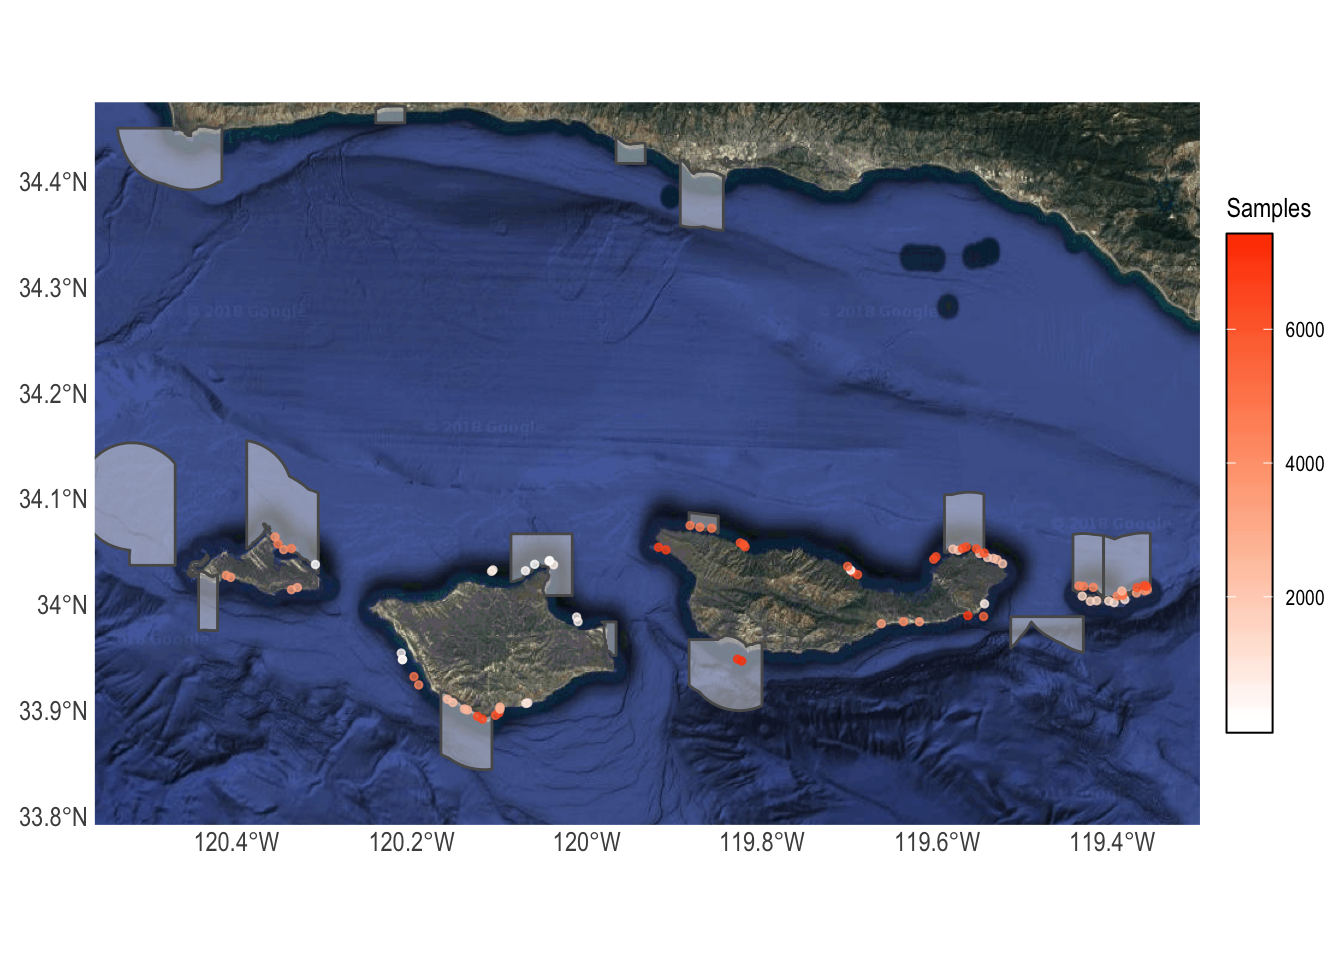
\includegraphics{thesis_files/figure-latex/ci-map-1.pdf}
\caption{\label{fig:ci-map}Map of study region and sampling locations.
Shaded polygons indicate location of MPAs. Points represent sampling
locations, and color indicates the number of observations recorded at a
given point}
\end{figure}
As we seek to understand the regional scale effects of MPAs, and as the
size of those regions increases, the harder it becomes to find a
practical control for the treated region. As a result, it becomes
challenging to determine what post-MPA changes throughout the region are
attributable to the MPAs and which to other factors. If abundance
continues to trend downwards post-MPA, without a control we cannot truly
know whether it might have trended down faster without the MPAs. Or, if
abundances are trending up, we cannot reliably say that the upward trend
is not due to some environmental driver. Regression analysis can help
(e.g.~statistically controlling for El Niño), but depends on ``selection
on observables'', meaning that in order to interpret the MPA
coefficients as causal, we have to assume that we have included all the
correct covariates that might also be correlated with the outcome of
interest (in this case abundance of fish). Failure to account for some
important variable in our regression can bias results.

We have then two broad options for estimating the regional effect of
MPAs in a place like the Channel Islands: We can depend on selection on
observables through regression analysis, or we can find an
identification strategy. Given the shortcomings of the first approach,
we propose an identification strategy building off of Caselle \emph{et
al.} (\protect\hyperlink{ref-Caselle2015}{2015}), in which we consider
relatively non-targeted species such as Garibaldi (\emph{Hypsypops
rubicundus}) to be ``controls'' for targeted species such as Kelp Bass
(\emph{Paralabrax clathratus}). Under this strategy, our assumption is
that non-targeted species are more or less unaffected by the
implementation of MPAs (unlike the targeted species), but that both
species are potentially affected by regional environmental trends. In
this way, the non-targeted species can serve as our control for
environmentally driven shifts in abundance that are not explicitly
controlled for in the model (as opposed to a selection on observables
approach), allowing us to attempt to better isolate changes in abundance
driven by MPAs from changes caused by environmental conditions.

\section{Results and Discussion}\label{results-and-discussion}

\subsection{Predicting Regional Effects of
MPAs}\label{predicting-regional-effects-of-mpas}

We used a bio-economic model to simulate the regional effects of MPAs
across 20,000 simulated fisheries spanning a wide range of plausible
states of nature, including degrees of larval and adult movement,
density dependence, fleet dynamics, life history, and pre-MPA
exploitation levels, each simulation representing a different state of
nature. For simplicity, at this point we focus on single species
outcomes, though since we do not model species interactions, fisheries
could be together to provide multi-species MPA effects. It is critical
to note that we have no current way of assigning probabilities to any of
these states of nature, though we have tried to constrain the parameter
space to plausible states. Therefore, the results of our simulations
suggest simply the number of simulated ways that a given outcome could
happen; we do not have any knowledge though if in reality some of these
simulated outcomes are individually much more or less likely than
others. But, if we assume that the simulated parameter space is a
reasonable representation of a range of plausible states of nature,
these results provide an indication of the general magnitude of effects
that we might expect.

Across this range of scenarios, we see that the median simulated
equilibrium regional effect (percentage change in total biomass) was
15\%, with a min of -95\% and a max of over 200\%. We also see that
while large percentage increases in biomass can accrue relatively
rapidly under some circumstances, increases of over 10\% took
approximately 10 years to achieve for 50\% of the simulated fisheries
(Fig.\ref{fig:trend-effect}). It is also clear from the simulations that
even constrained by reasonable states of nature, a vast array of
regional conservation MPA effects are possible. The exact expected
regional effect for a given fishery will depend on a complex set of
interactions among fishery variables. However, two of the most critical
factors affecting the direction and magnitude of the regional effect are
the degree of overfishing (displayed in plots as initial depletion, with
greater overfishing resulting in higher depletion) present before (and
continuing after) MPA implementation, and the size of the MPA, and so we
focus on the effects of these two variables on regional MPA effects 15
years after MPA implementation (to mimic the time since implementation
of the Channel Islands MPAs at the time of this publication). Across our
simulated fisheries, the median 15 year simulated regional effect was
4\%. For cases where ``small'' MPAs (smaller than 25\%) were implemented
in relatively unexploited fisheries (depletion \textless{} 50\%), the
median regional effect was 0\%. For moderate depletion (50\% to 75\%),
MPA sizes from 1\% to 50\% produced median MPA effects of 3\%, while for
depletion above 75\% the median regional effect from was 80\%
(Fig.\ref{fig:f-and-s-plot}-A). The median regional effect increased
with both MPA size and depletion, but it is important to note that the
ranges around these median values are extremely wide
(Fig.\ref{fig:f-and-s-plot}-B). Broadly, the simulation results show
that integrating across a broad set of states of nature defined by
theoretical drivers of MPA effects, under most simulations the MPAs
produced positive effects, though smaller effects were much more likely
than large effects. In some instances though, MPAs actually resulted in
net regional conservation losses. While factors such as MPA size and
pre-MPA depletion are critical drivers, we also show that controlling
for these a wide range of outcomes are still possible
(Fig.\ref{fig:f-and-s-plot}).
\begin{figure}
\centering
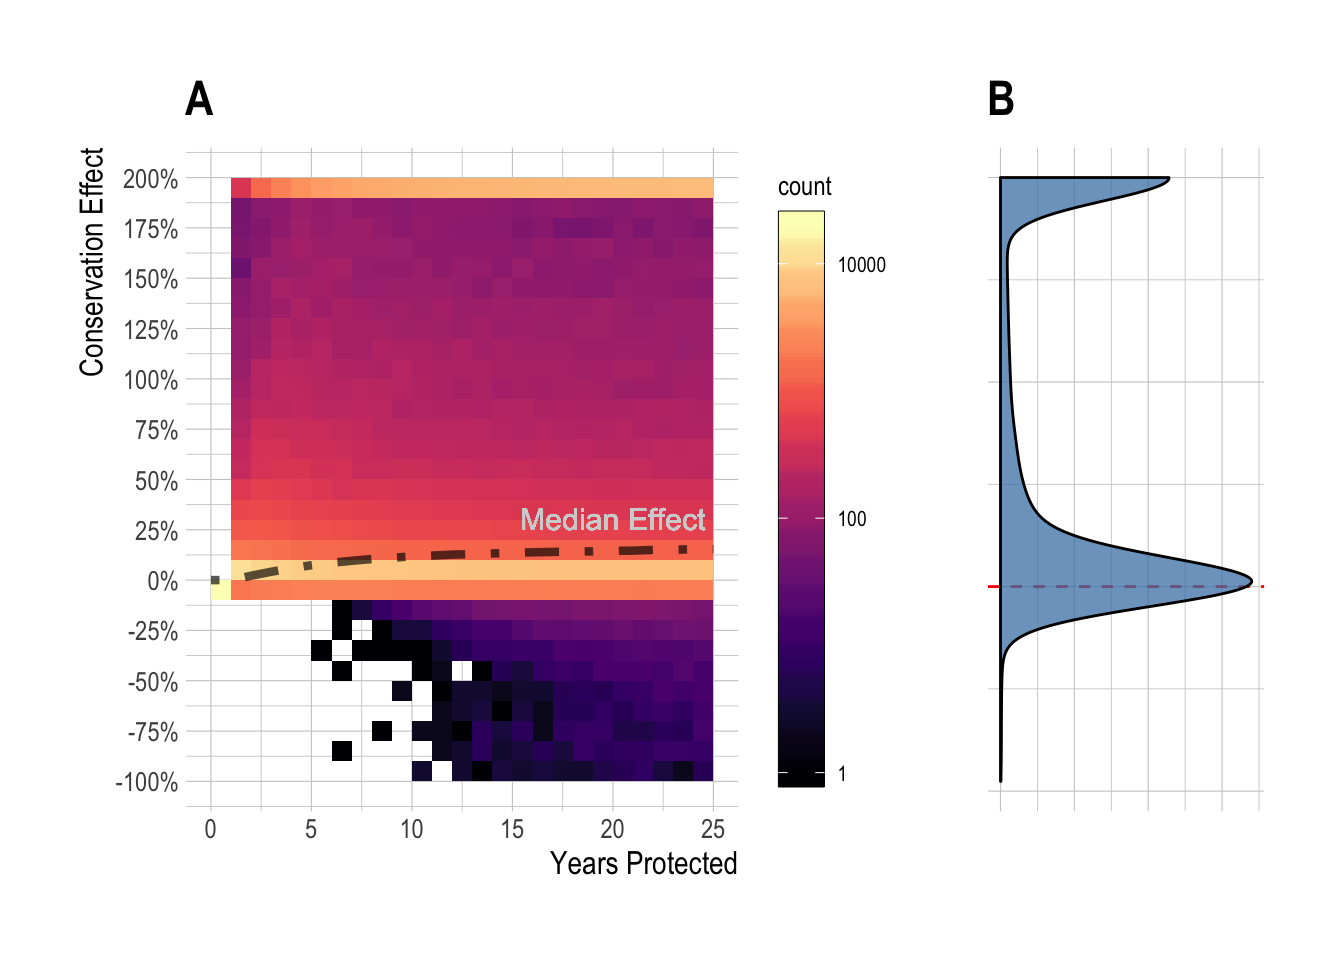
\includegraphics{thesis_files/figure-latex/trend-effect-1.pdf}
\caption{\label{fig:trend-effect}Distribution (and median, black line) of
simulated regional MPA effects over time (A), and at equilibrium (B).
Color indicates number of simulations at a binned effect size at a given
time (note log-10 scale of color fill for visual clarity).}
\end{figure}
\begin{figure}
\centering
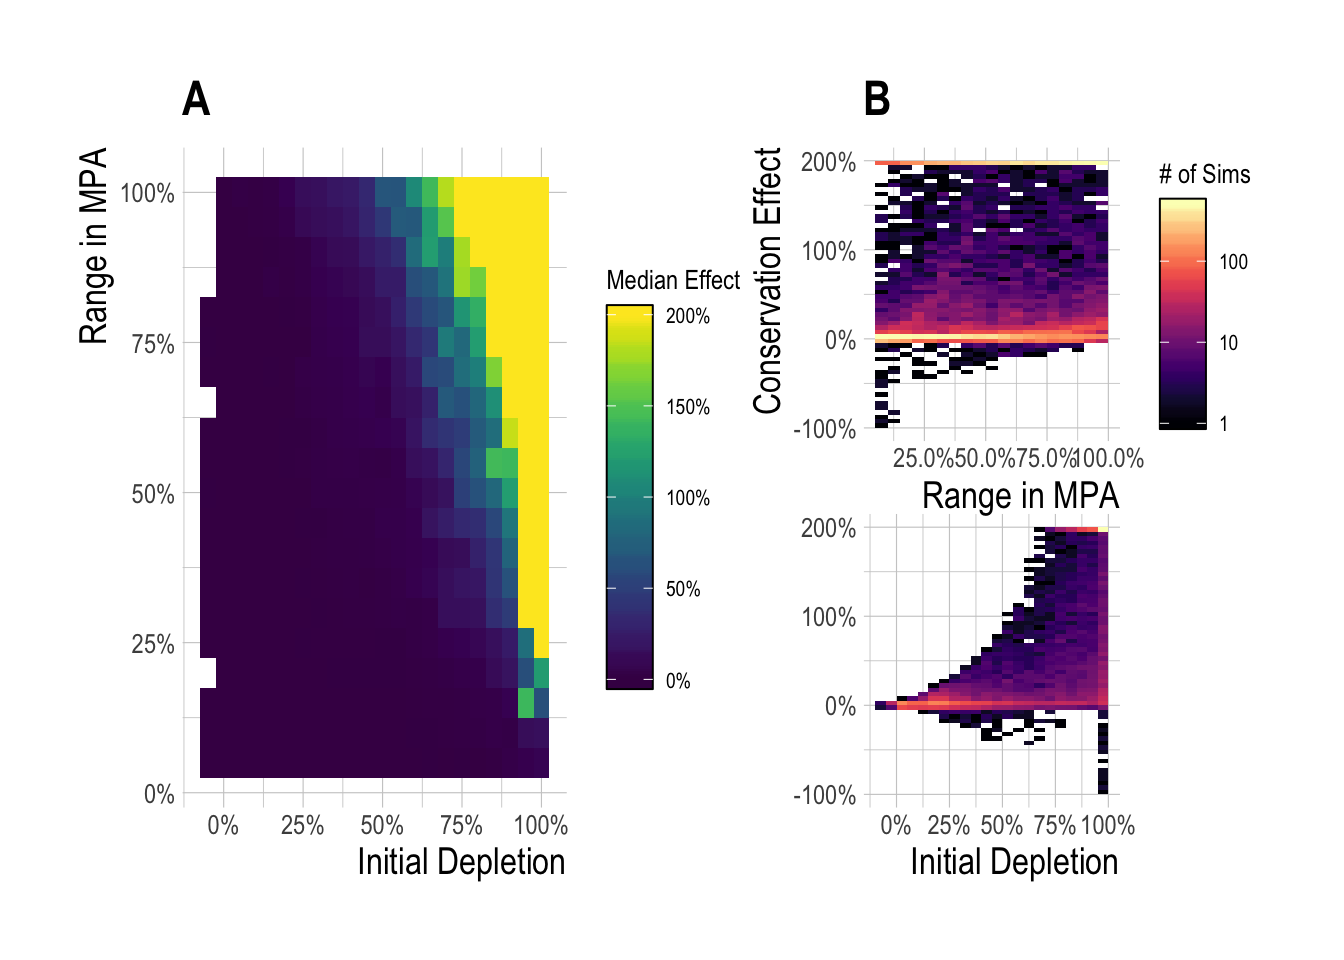
\includegraphics{thesis_files/figure-latex/f-and-s-plot-1.pdf}
\caption{\label{fig:f-and-s-plot}Median (A) and range of (B) regional MPA
effect after 15 years of protection across a range of pre-MPA depletions
and MPA sizes}
\end{figure}
The percentage change in biomass with and without MPAs is most analogous
to the effects that can (in theory) be estimated by our identification
strategy (the percentage difference in the density of targeted species
relative to the non-targeted species pre and post MPA). However, the
percentage change in biomass is a somewhat misleading metric from the
perspective of meaningful conservation outcomes. Take for example an
extremely depleted scenario where without MPAs a fishery is left with
only 2 kg of fish. Suppose then that an MPA brings us up to 6 kg of
fish, and that the unfished biomass in this fishery is 1,000kg. While
the MPA has produced a 200\% increase in fish biomass, this increase is
relatively inconsequential given the scale of the population (we have
only recovered 0.4\% of the unfished biomass), and likely to be very
challenging to detect in a real ecological system.

To reflect this, we can repeat the analyses in
Fig.\ref{fig:trend-plot}-\ref{fig:f-and-s-plot}, but now expressing the
change in biomass with and without MPAs as a percentage of unfished
biomass for that fishery. Through this metric, we see median equilibrium
effect sizes of 2\% (Fig. \ref{fig:pop-trend-effect}). Over the 15 year
time horizon, our simulations find that MPAs less than 25\% produced a
median effect of near 0\% (Fig. \ref{fig:pop-f-and-s-plot}-A), but again
with a wide range around the simulated outcomes outcomes, from -20\% to
100\% (Fig. \ref{fig:pop-f-and-s-plot}-B).
\begin{figure}
\centering
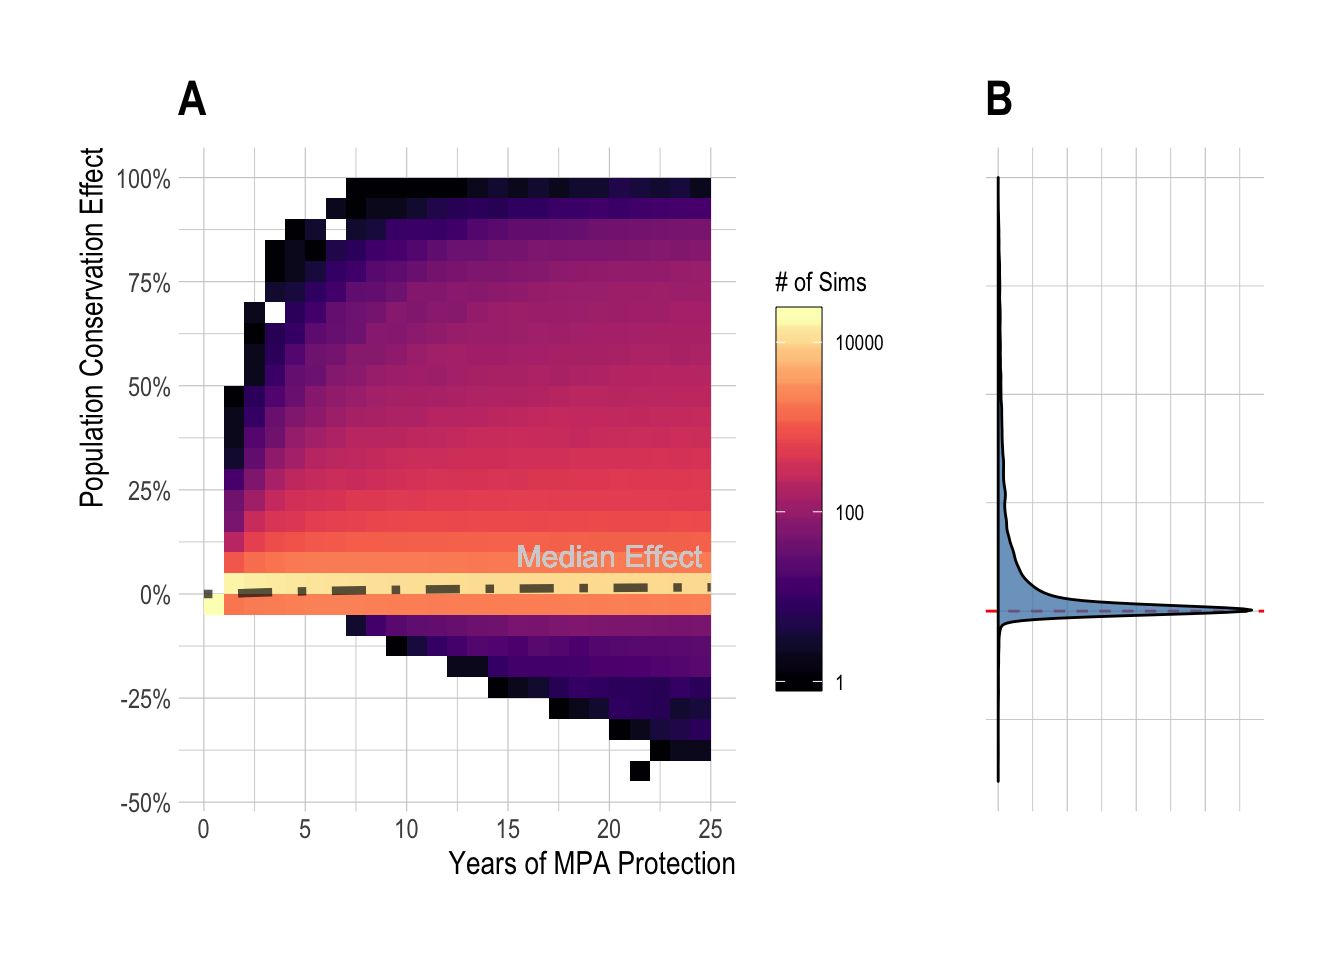
\includegraphics{thesis_files/figure-latex/pop-trend-effect-1.pdf}
\caption{\label{fig:pop-trend-effect}Distribution (and median, black line)
of simulated regional MPA effects (expressed as percent of unfished
biomass) over time (A), and at equilibrium (B)}
\end{figure}
\begin{figure}
\centering
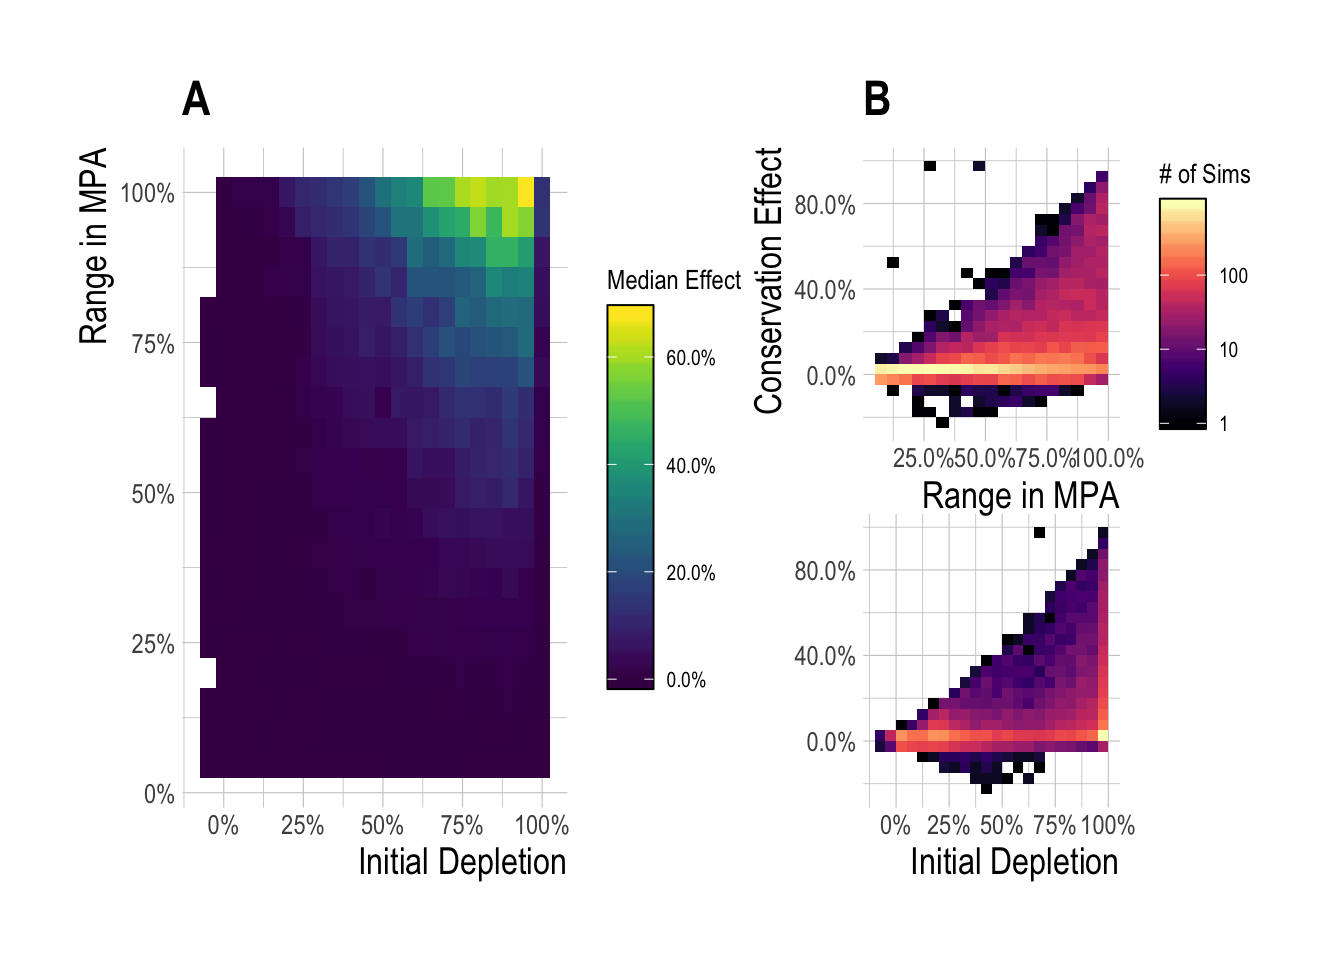
\includegraphics{thesis_files/figure-latex/pop-f-and-s-plot-1.pdf}
\caption{\label{fig:pop-f-and-s-plot}Median (A) and range (B) regional MPA
effect (expressed as percent of unfished biomass) after 15 years of
protection across a range of pre-MPA depletions and MPA sizes}
\end{figure}
Readers may be especially interested in the simulated scenarios that
produced negative MPA effects. The constant-catch fleet model was one of
the most important drivers of extremely negative MPA effects, especially
when both depletion and MPA size were in the 25-50\% range
(Fig.\ref{fig:fleet-plot}). A decision tree analysis conducted using the
\texttt{rpart} package through \texttt{caret} confirms that the primary
drivers of negative population outcomes are constant-catch dynamics
interacting with the size of the MPAs (Fig.\ref{fig:neg-tree}). As the
name implies, under the constant-catch fleet model fishing communities
seek to catch the same amount regardless of the presence of an MPA.
While a constant catch greater than MSY is not possible over the
long-term under the confines of this simulation framework (the
population would crash), over the short-term a constant-catch scenario
is not a particularly outlandish idea. Subsistence fisheries may conform
to a constant-catch style policy over the short-term, as they seek to
ensure the nutritional needs of their community. More industrial
fisheries may have pre-arranged purchase orders for levels of catch.
Quota managed fisheries may maintain relatively static quota levels
until new stock assessments can be completed. The key outcome of these
results is that the regional conservation effects of an MPA are
critically dependent on fisheries management institutions outside the
protected areas; an MPA that would provide large benefits under
open-access dynamics may actually harm conservation in a constant-catch
scenario.
\begin{figure}
\centering
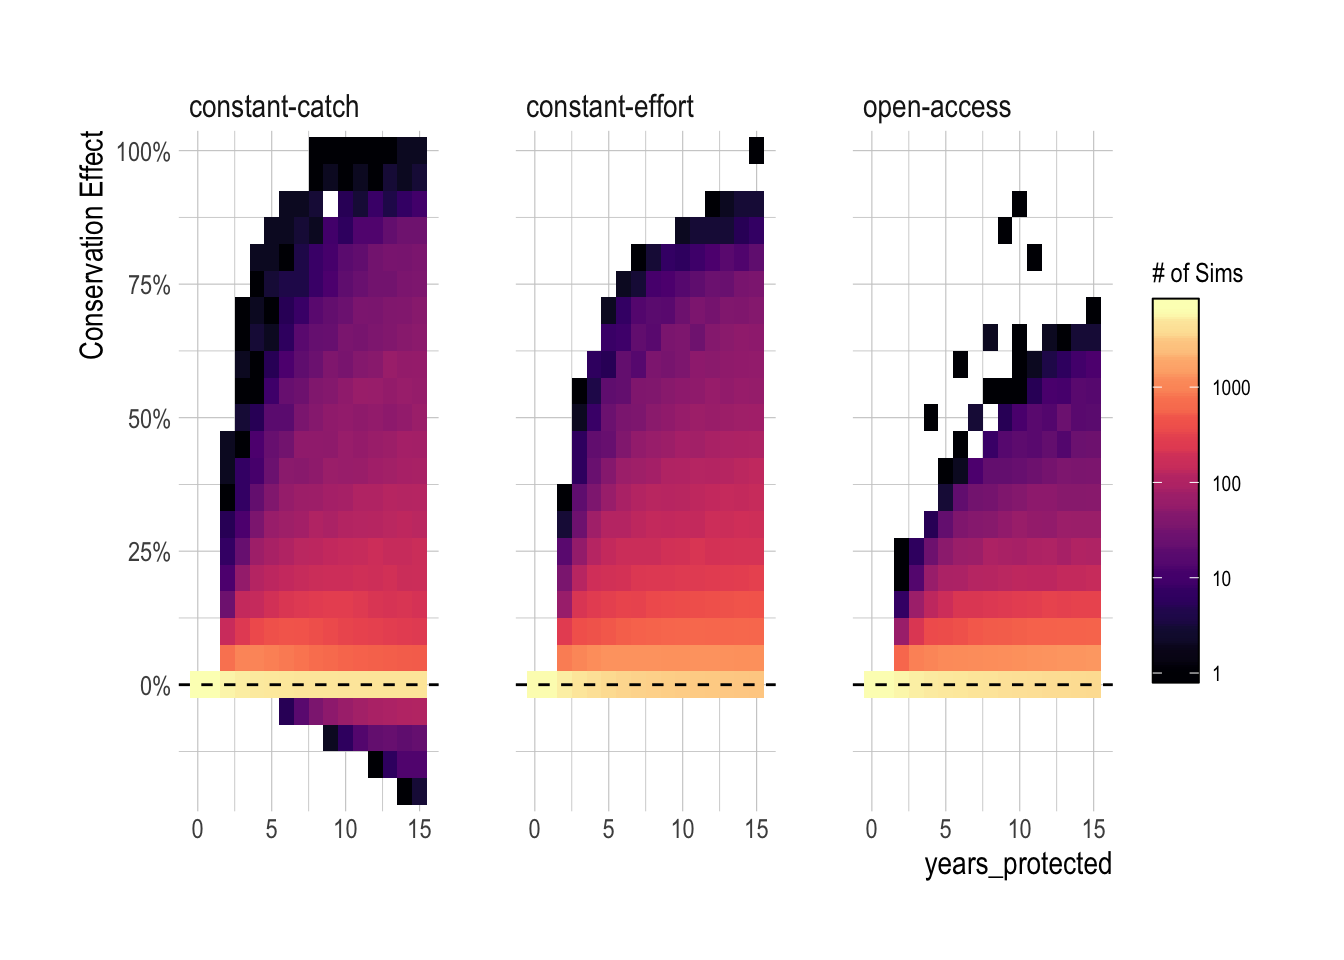
\includegraphics{thesis_files/figure-latex/fleet-plot-1.pdf}
\caption{\label{fig:fleet-plot}Density plot of regional conservation MPA
effect by fleet model}
\end{figure}
\begin{figure}
\centering
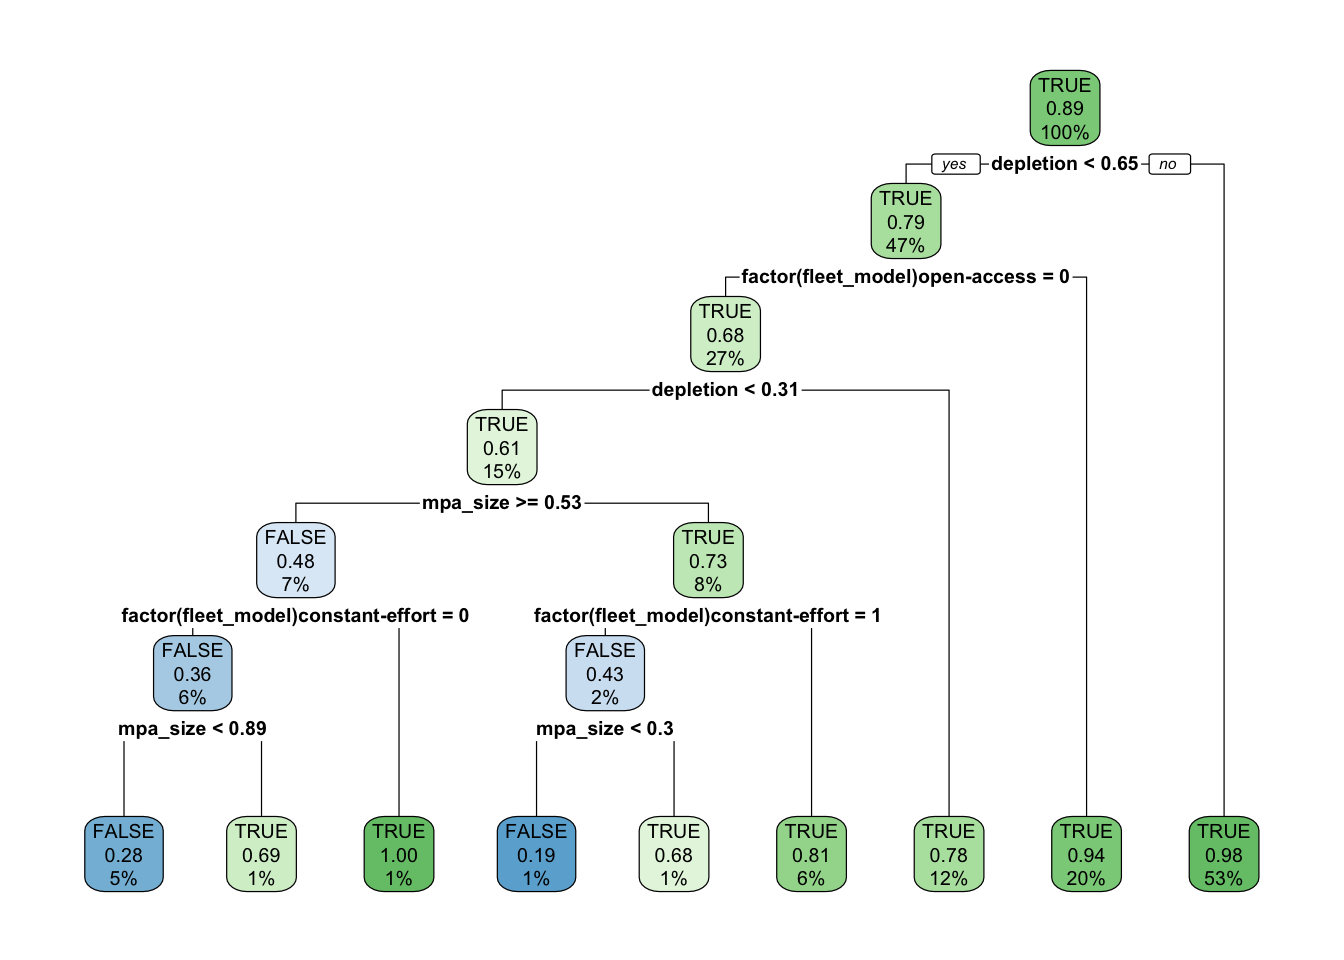
\includegraphics{thesis_files/figure-latex/neg-tree-1.pdf}
\caption{\label{fig:neg-tree}Classification tree of positive MPA effects as
a function of simulation traits. TRUE indicates that the model predicts
there to be a positive regional MPA effect, FALSE a negative effect.
Decimal numbers show predicted probability of positive MPA effects,
percentages the percent of observations at a given level that fall in
that node. Intensity of color is proportional to confidence in
prediction (decimal number)}
\end{figure}
\subsubsection{Fishery Effects of MPAs}\label{fishery-effects-of-mpas}

While the emphasis of this particular research project is on predicting
and detecting the regional conservation effects of MPAs, the simulation
framework that we have constructed also allows us to consider the
fishery effects of MPAs, as defined by the percentage gain or loss in
total fishery catches following the implementation of MPAs, relative to
what the (simulated) fishery would have caught in that scenario without
the MPAs. We omit the constant-catch fleet model from this assessment,
since by definition (in the short-term at least), catches are the same
with or without MPAs (though effort required to obtain those catches,
and therefore profits, could be quite different). Similar to the
conservation effects, we examined both the median and range of effects
as a function of pre-MPA depletion and MPA size. Expressed as a
percentage difference in catches with and without MPAs, across our
simulated fisheries the median fishery effect for MPA sizes less than
25\% and for depletion's less than 75\% (\textasciitilde{} B/Bmsy
\textgreater{} than 0.6, Assuming Bmsy/K of 0.4) was near 0\%. The
median fishery effect when depletion was above 80\% was commonly near
100\%. However, for MPA sizes greater than 25\% and for depletion's less
than 75\%, the median MPA effect on fishery catches was negative.
Pre-MPA depletion was the clearest driver of the magnitude and direction
of MPA fishery effects. Meaningful numbers of simulations experienced
positive fishery effects only once depletion's exceeded 50\%, with a
substantial ramp-up of positive effects after 75\%. While both
substantial positive and negative effects were possible over a range of
MPA sizes, as MPA size passes 50\% most simulations start to produce
negative fishery effects (Fig.\ref{fig:catch-effects}).
\begin{figure}
\centering
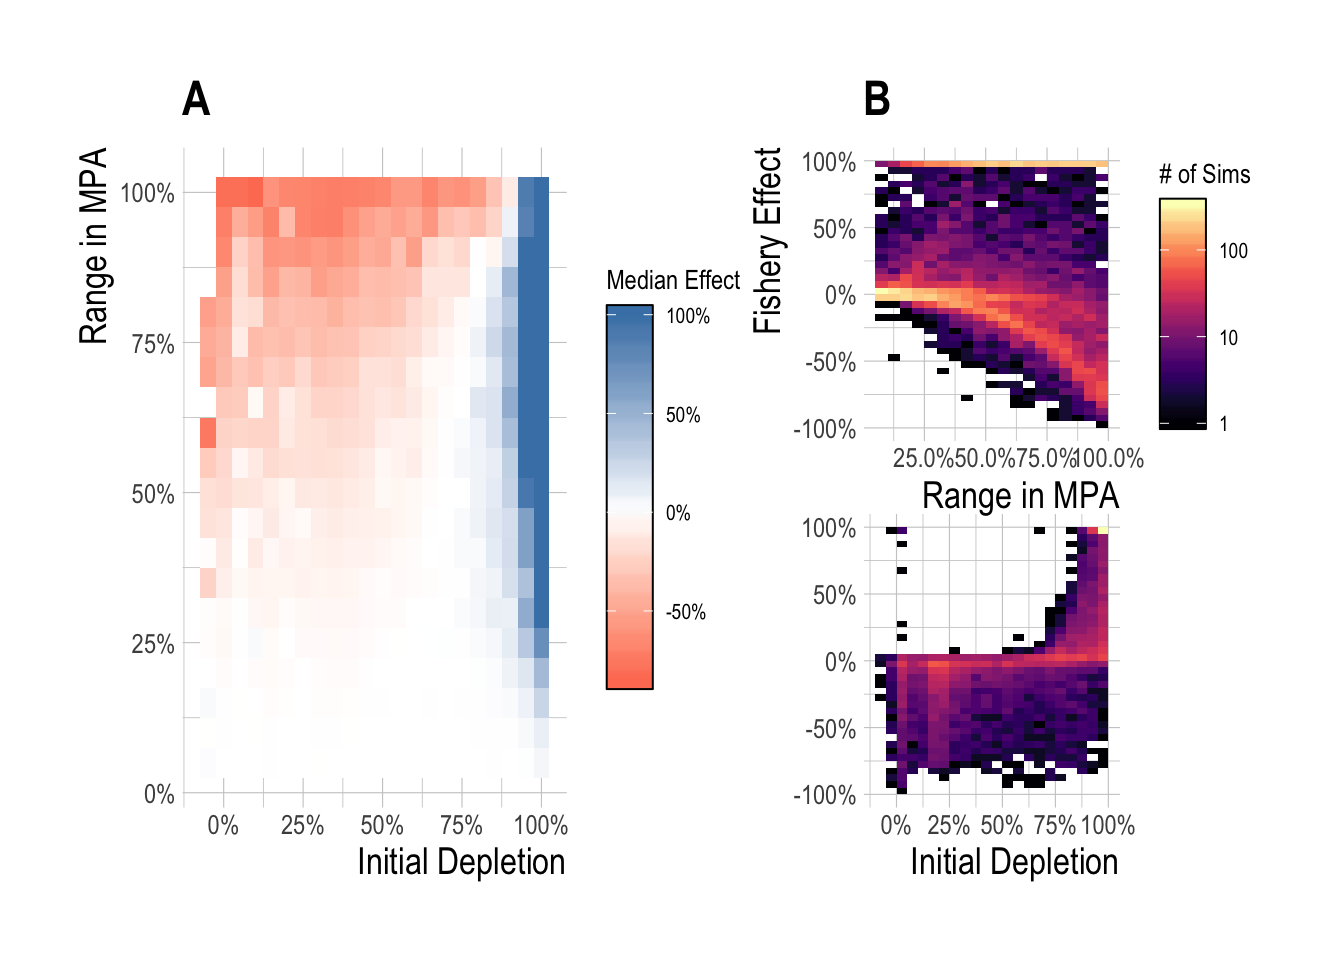
\includegraphics{thesis_files/figure-latex/catch-effects-1.pdf}
\caption{\label{fig:catch-effects}Median (A) and range (B) fishery effect
(percentage change in catch with and without MPAs) after 15 years of
protection across a range of pre-MPA depletions and MPA sizes}
\end{figure}
Many of the large percentage changes in this analysis can be attributed
to very small catches in the absence of MPAs. Catches are generally
quite low once a fishery has been collapsed, and so when depletion was
near 100\%, catches were small, and so a relatively small change in
absolute catch following MPA implementation can produce large percentage
changes. To address this, we also scaled the differences in fishery
catches with and without MPAs by the maximum sustainable yield for that
simulated fishery. The fishery effect now reflects the percentage of MSY
gained or lost as a result of MPA implementation. The overall trends are
similar to the relative change in catch results, but the 15 year effects
are more muted, with peak positive effects near 25\% and negative
effects near -75\% (Fig.\ref{fig:catch-msy-effects}).
\begin{figure}
\centering
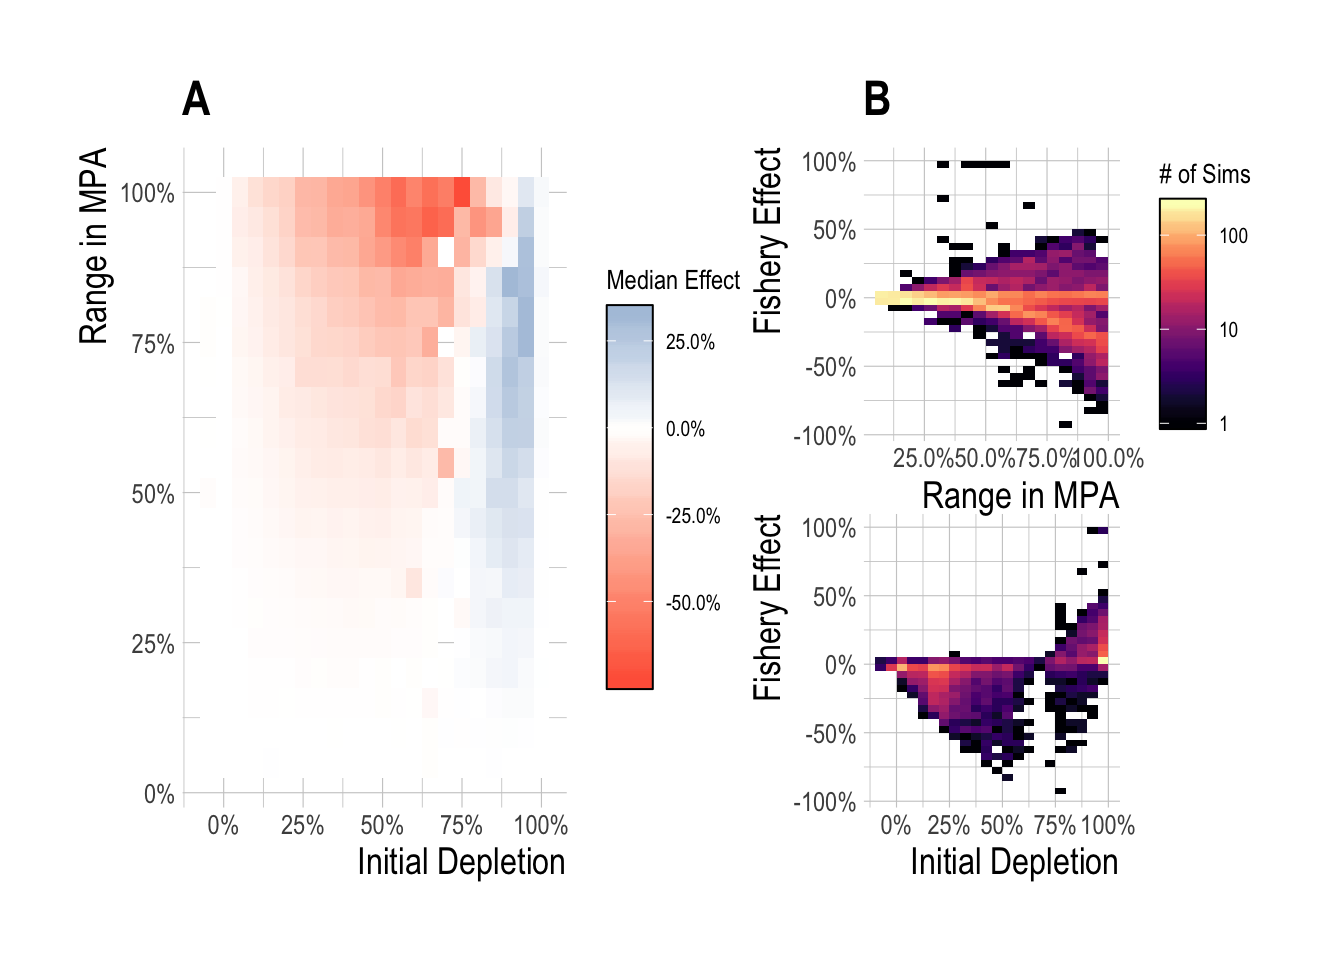
\includegraphics{thesis_files/figure-latex/catch-msy-effects-1.pdf}
\caption{\label{fig:catch-msy-effects}Median (A) and range (B) fishery
effect (percentage change in catch with and without MPAs relative to
MSY) after 15 years of protection across a range of pre-MPA depletions
and MPA sizes}
\end{figure}
\subsection{Detecting Regional MPA
Effects}\label{detecting-regional-mpa-effects}

Theory and simulation testing indicate then that while the regional
effects of MPAs can range from strongly negative to highly positive,
with the bulk of scenarios producing 0-10\% regional conservation
effects after fifteen years of protection (though much more negative and
much more positive outcomes are certainly possible). Given this, our
expectation is that the ``true'' regional effect will likely be
challenging to isolate from the variation of natural systems in and the
observation error inherent to any MPA monitoring program. We use data
from the Partnership for Interdisciplinary Studies of Coastal Oceans
(PISCO) monitoring of the Channel Islands National Marine Sanctuary to
test our ability to detect the regional effect of MPAs in a real world
context. PISCO conducts visual underwater SCUBA surveys at a variety of
rocky-reef and kelp forest sites inside and outside of MPAs throughout
the Channel Islands. At the rawest level, the data are counts of finfish
in 2cm length bins along a 30m x 2m transect at various sites and
depths. These length bins are converted to biomass, and then biomass
densities, by converting length to weights using available allometric
data and dividing by the transect area. Our goal then is to estimate the
effect of the MPAs on these densities of fish throughout the Channel
Islands.

Our identification strategy for this case study is to use non-targeted
species as our control for unaccounted for environmental trends before
and after MPA implementation (which occurred in 2003). The model
estimates the difference in the trends between targeted and non-targeted
species pre- and post-MPA. We hypothesize that there should be no
difference in pre-MPA trends. We fit this model using a hierarchical
mixed-effect framework using Template Model Builder (TMB, Kristensen
\emph{et al.} \protect\hyperlink{ref-Kristensen2016}{2016}) in R (R Core
Team \protect\hyperlink{ref-RCoreTeam2018}{2018}). The model consists
broadly of three levels, the first (starting from the ``bottom'') being
transect-level densities of fish species observed by PISCO, which are
standardized into a unit-less index of biomass abundance (which we will
refer to as an abundance index from now now), accounting for both
probability of detection and expected density as a result of changes in
both abundance and covariates such as observer skill (see Maunder and
Punt \protect\hyperlink{ref-Maunder2004}{2004}). For the second stage,
we break the abundance indices into targeted and non-targeted species
(per the classifications in the PISCO data), and estimate the mean trend
of each group (targeted and non-targeted) over time. In the third step,
we estimate the difference in the mean trend between the targeted and
non-targeted fishes, which under the right set of circumstances should
reflect the causal effect of the MPAs on the outcome of interest (in
this case regional biomass density of targeted fishes). It is important
to stress that all three of these steps are integrated into the same
estimation model, in order to propagate uncertainty through the model
correctly.

We tested this estimation model against simulated data to ensure that,
if our assumptions are satisfied, our identification strategy works
correctly. For the simulation study, we attempted to replicate the key
characteristics of the PISCO data (omitting the probability of detection
portion of the model due to logistical complexity). Using the same
species that we include in the true analysis, we simulate divers of
varying and evolving skill conducting visual transect surveys to obtain
estimates of length composition, which are then converted into biomass.
Using the measured temperature trends in the Channel Islands over the
time period of the study, simulated recruitment deviates of northern
species are negatively affected by warmer water, southern species
positively affected. Unfished species are unaffected by MPAs. We then
fit our estimation model to these simulated data to test our
identification strategy, and we found that our proposed estimation
strategy is able to recover the true mean simulated MPA effect
(Fig.\ref{fig:sim-tests}).
\begin{figure}
\centering
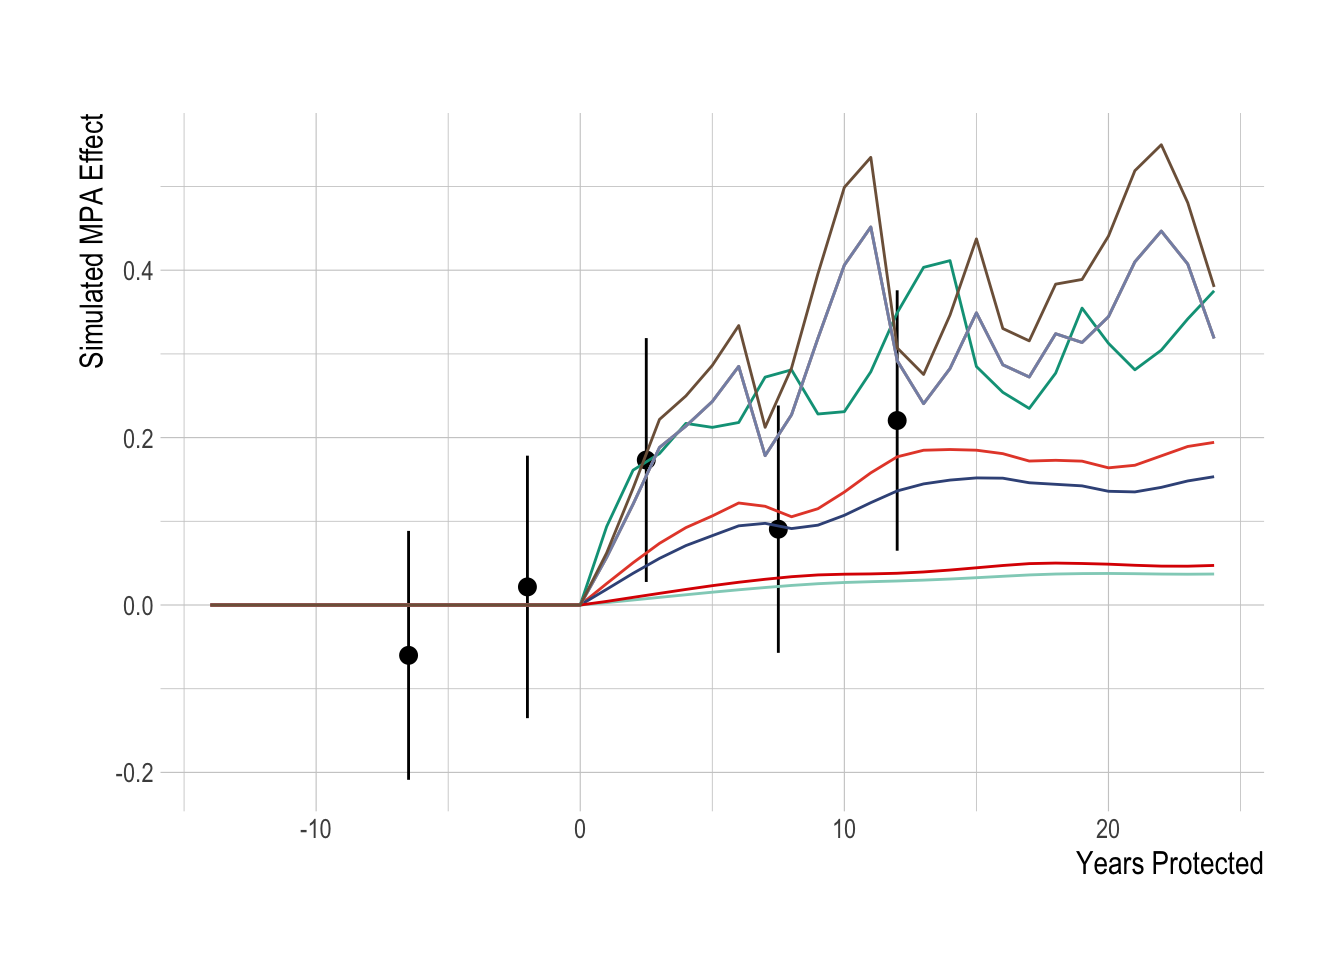
\includegraphics{thesis_files/figure-latex/sim-tests-1.pdf}
\caption{\label{fig:sim-tests}Simulation testing of identification strategy.
Colored lines show true MPA effect for simulated targeted species. Black
points represent mean estiamted regional MPA effect over 5-year blocks
(range indicate 95\% confidence interval)}
\end{figure}
Since we have evidence that our estimation model functions if its
assumptions are satisfied, we then turned to estimating the regional MPA
effect from the PISCO data. While individual species in the survey have
their own abundance trends, the model assumes that abundance of targeted
and non-targeted species each come from a common distribution. Assuming
parallel pre-treatment trends, which visual (Fig.\ref{fig:raw-trend})
and statistical (Fig.\ref{fig:did-plot}) assessment do not rule out, the
trend in the underlying mean abundance index of non-targeted species
post MPA serves as our control for unobserved environmental variables
that could also affect the trends in the mean density of targeted
species. So, by this logic, we should see no significant divergence
between the targeted and non-targeted abundance trends pre ``treatment''
(implementation of the MPAs), and then some divergence between the
treated group (targeted species) and the non-treated group
(non-targeted) post treatment (if the treatment has an effect).

Under these idealized circumstances, the magnitude of this divergence
between the treated (targeted) and non-treated (non-targeted) groups
post treatment is an estimate of the causal effect of the treatment (the
implementation of MPAs). It is important to consider what exactly this
model controls for (and what it does not). Under the parallel trends
assumption, we assume that both the targeted and non-targeted fishes
respond the same way to non-modeled environmental drivers. For example,
the Channel Islands region experienced a major El Niño event from 2014
to 2016. While we include variables such as deviations from each
specie's preferred thermal niche, along with kelp cover, in our model,
these are clearly not the only factors affected by El Niño. However, if
the parallel trends assumption is correct, the El Niño effects that are
not explicitly included in the model are controlled for by the trend of
the non-targeted fishes.

However, this clearly does not control for differences in responses to
non-modeled variables between the treated and non-treated groups. For
example, the model only pre-MPA data from 2000 through 2002. The
parallel trends assumption appears plausible over that time period
(Fig.\ref{fig:did-plot}). But, this pre-treatment period does not
include an El Niño, while the post-treatment period does. Therefore,
while the parallel trends assumption looks plausible from the
pre-treatment data, it is possible that targeted and non-targeted fishes
respond in a systematically different manner to El Niño, therefore
violating the parallel trends assumption and invalidating the ``causal''
interpretation of the model. Similarly, the model cannot account for
additional shocks to the targeted species beyond the MPAs. For example,
while we control for total landings of each targeted species in the
Santa Barbara region, it is possible that within that region fishing
effort became increasingly concentrated around the Islands, driving down
local densities of fished species. The model cannot control for this
unless the appropriate data are correctly incorporated into the model
explicitly (and these data were not available at the time of this
study).

The model also assumes that the targeted and non-targeted fishes do not
directly or indirectly affect each other. This assumption is clearly
violated on some level: all the fishes in this analysis are part of the
same ecosystem and therefore interact to some degree. For example, if
the protection of targeted predatory fishes results in increased
mortality of non-targeted fishes, the model would attribute that as an
increased regional effect (greater divergence between the abundance of
targeted and non-targeted species). Given the time scale of analysis (15
years of protection), we do not feel that massive trophic cascades are
likely to have developed yet, given both the pace and complexity of
trophic cascade development (Babcock \emph{et al.}
\protect\hyperlink{ref-Babcock2010}{2010}; Pershing \emph{et al.}
\protect\hyperlink{ref-Pershing2015a}{2015}). A complete assessment of
evidence for trophic cascades in the Channel Islands is beyond the scope
of this study, but to address this question somewhat we utilized
convergent cross mapping sensu Sugihara \emph{et al.}
(\protect\hyperlink{ref-Sugihara2012}{2012}) to test for a significant
causal signal between different broad trophic groups in the data,
implemented in the \texttt{rEDM} package in R.

Following methods laid out in Clark \emph{et al.}
(\protect\hyperlink{ref-Clark2015}{2015}), we pool the abundance of each
broad trophic group by region (Fig.\ref{fig:trophic-plot}. This uses the
data from the islands as ``replicates'', requiring the assumption that
the islands are all part of the same dynamic system, but allowing us to
take advantage of the extra information provided by each island to
further resolve the reconstructed manifolds. Using these aggregations,
we then test whether the variables can be properly embedded, i.e., if
they have predictable manifold dynamics. We do this through a simplex
forecasting test, using an individual timeseries' own lags to build a
manifold. For each timeseries, the ``best embedding dimension'' is an
approximation of the dimensionality of the dynamic system, in other
words, the number of dimensions that define and predict the evolving
states of the timeseries. This analysis shows that only the carnivore
and herbivore groups show evidence of predictability within the
timeseries (skill approaching zero within the tested embedding
dimensions, Fig.\ref{fig:embed-plot}).
\begin{figure}
\centering
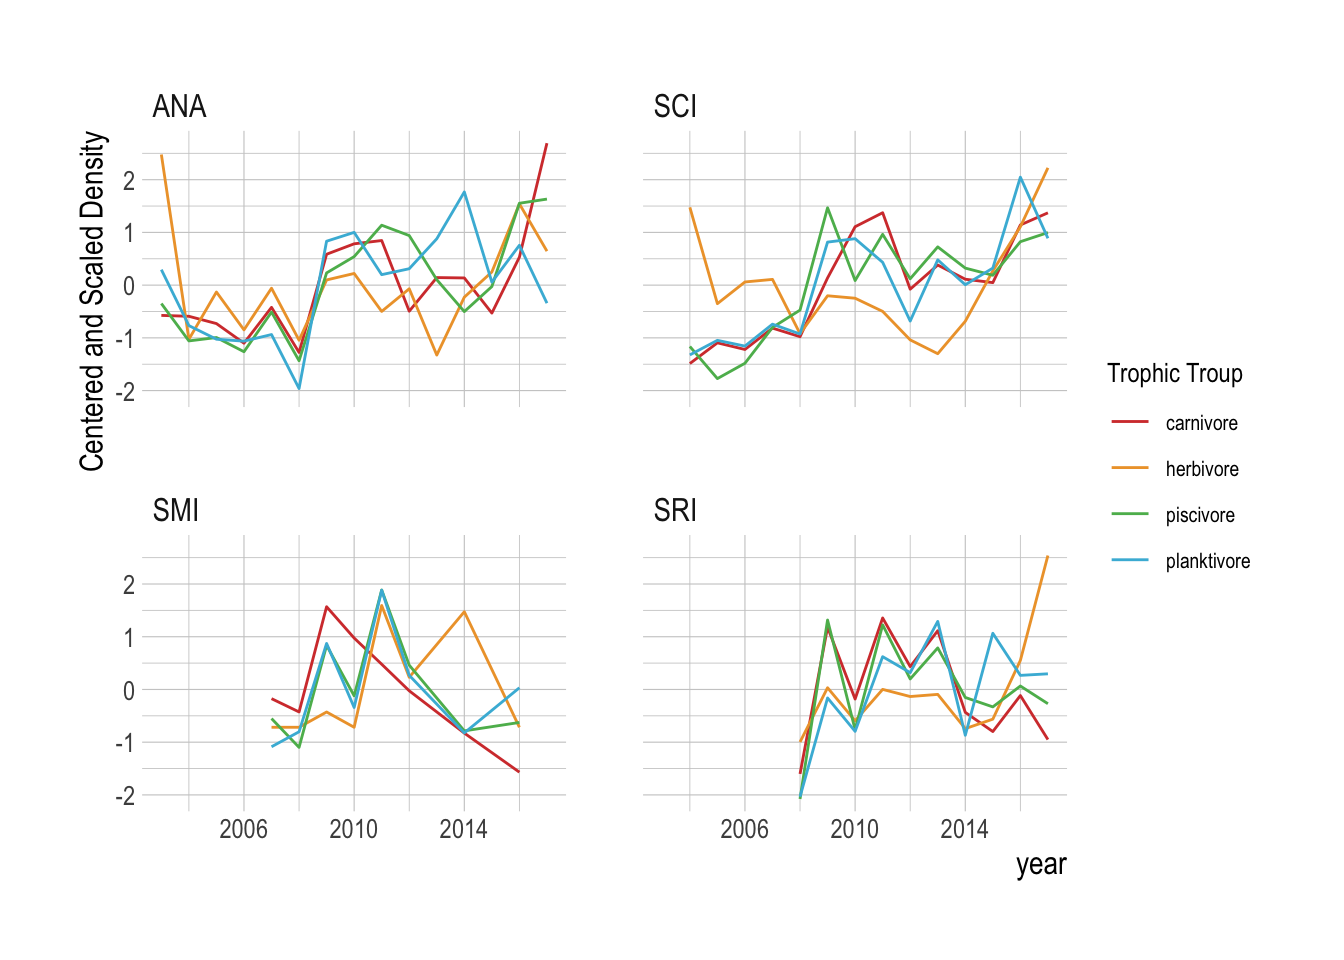
\includegraphics{thesis_files/figure-latex/trophic-plot-1.pdf}
\caption{\label{fig:trophic-plot}Centered and scaled densities by broad
trophic group and island over time}
\end{figure}
\begin{figure}
\centering
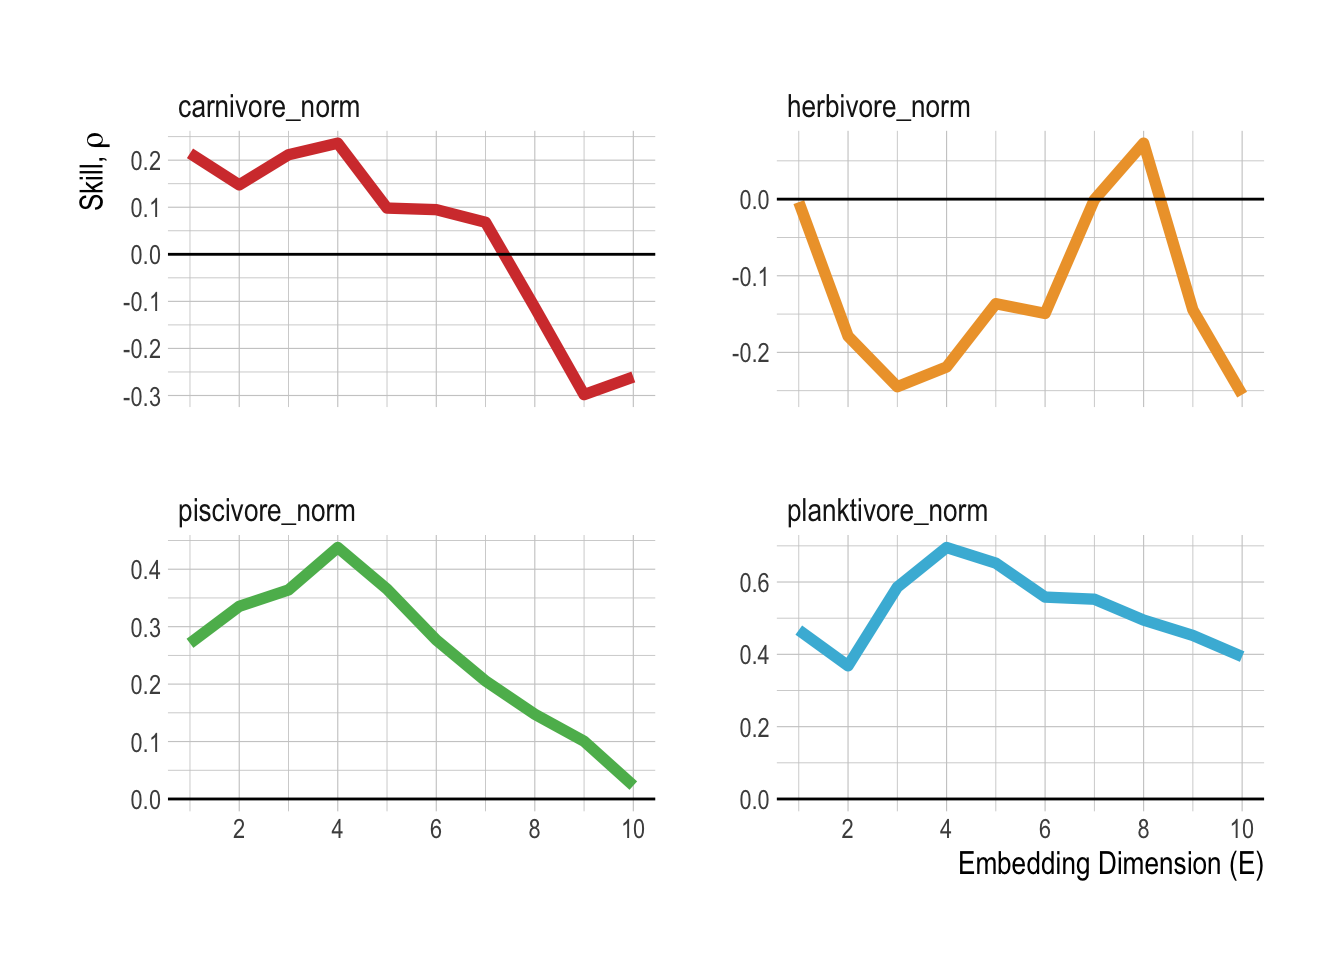
\includegraphics{thesis_files/figure-latex/embed-plot-1.pdf}
\caption{\label{fig:embed-plot}Predictive skill as a function of embedding
dimensions}
\end{figure}
Focusing on just these two groups then, we can test for a causal
relationship through Takens theorem using convergent cross mapping.
Generalizations of Takens' theorem indicate that if two variables (in
our case, species or physical variables) are part of the same dynamic
system, their individual dynamics should reflect their relative causal
influence. In other words, if one variable is causally forced by
another, that forcing should leave a signature on the first time series.
Convergent cross mapping (CCM) tests for causation by using the
attractor/manifold built from the time series of one variable to predict
another (hence the ``cross-mapping''). In simple terms, the \emph{causal
effect of A on B is determined by how well B cross-maps A}.

There are two criteria for CCM to establish causality: First, and most
obviously, predictive cross-map skill using all available data should be
significantly greater than zero. Second, that predictability should be
convergent. Convergence means that cross-mapped estimates improve with
library length (the number of state-space vectors used to build the
attractor), because the attractor is more fully resolved and therefore
estimation error should decline. Convergence is key to distinguishing
causation from simple or spurious correlation. If two variables are
spuriously correlated and not causally linked, CCM should fail to
satisfy this second criterion. Based on these criteria, there is some
slight evidence that herbivores may be driving carnivore densities, but
no evidence that carnivores drive herbivores (Fig.\ref{fig:cross-map}).
This analysis provides evidence that trophic cascades are unlikely to be
a significant driver of our results. It is important to note though that
this analysis does not mean that trophic cascades could not evolve,
rather that we do not detect them with these data at this time.
\begin{figure}
\centering
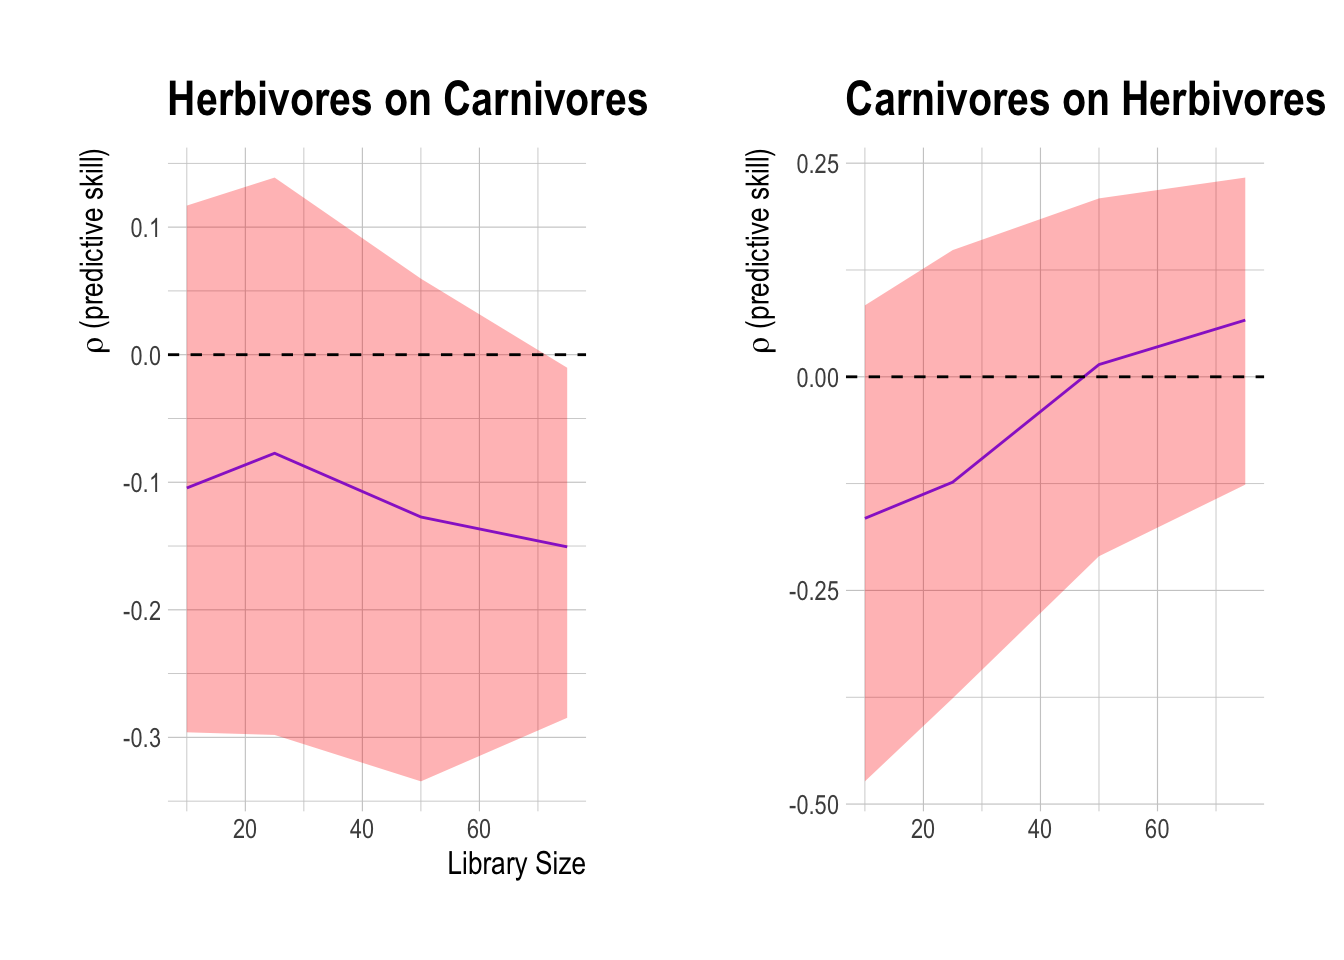
\includegraphics{thesis_files/figure-latex/cross-map-1.pdf}
\caption{\label{fig:cross-map}Cross mapping of effect of herbivores on
carnivores (A) and carnivores on herbivores (B) in the PISCO data from
2000 to 2017. Shaded region show 95\% confidence interval}
\end{figure}
The proposed identification strategy serves to control for some
unobserved factors influencing densities of targeted and non-targeted
species, but is unlikely to account for all of them. Before examining
regression results, we can graphically examine the trends in mean
densities for targeted and non-targeted species over time. We centered
and scaled the mean annual densities for each species included in the
analysis in order to compare the trends across species groups. Grouping
the species by targeted and non-targeted status, we see evidence of
pre-treatment parallel trends in the abundance indices, and of a
divergence post MPA implementation. Beginning in around 2007 abundances
of targeted species appear to start increasing faster than non-targeted
species. However, from 2012 onward abundances of targeted species appear
to be declining relative to the trend in the non-targeted species. Not
controlling for any other factors that may affect fish abundances, the
data suggests a possible increase in targeted species abundance
(relative to the ``control'' trend of the non-targeted species) at
first, followed by a decrease in the most recent years
(Fig.\ref{fig:raw-trend}).
\begin{figure}
\centering
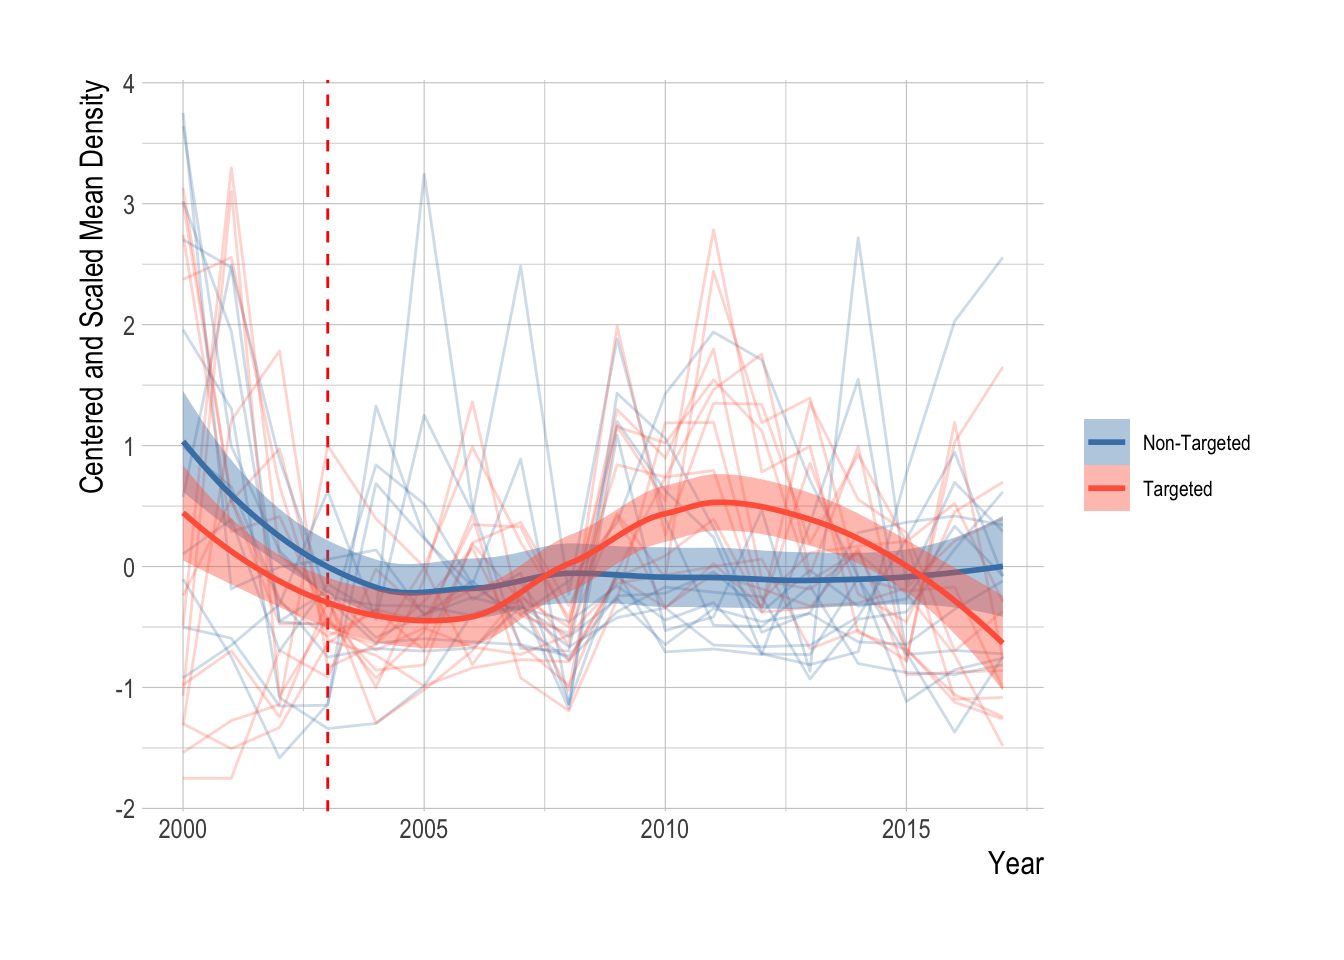
\includegraphics{thesis_files/figure-latex/raw-trend-1.pdf}
\caption{\label{fig:raw-trend}Centered and scaled mean annual density of
included species (faded lines) and smoothed means of targeted and
non-targeted groups (darker lines and ribbon representing 95\%
confidence interval of the mean) over time}
\end{figure}
We confronted these visual trends with our statistical analysis to
estimate the divergence in the abundance trends of targeted and
non-targeted fishes, controlling for factors such as observer effects,
kelp and temperature, and unobserved environmental drivers through the
parallel trends assumption. Using this analysis, we do not detect a
significant change in the density of targeted fishes relative to the
density of non-targeted fishes following the implementation of MPAs in
the Channel Islands in 2003 (Fig.\ref{fig:did-plot}). The mean estimated
post MPA implementation divergence between the trends of targeted and
non-targeted species was 0, indicating a roughly 0\% divergence.
However, it is important to note that just because we cannot a reject a
hypothesis of zero divergence between the targeted and non-targeted
groups does not mean that we have precisely estimated the effect size to
be zero. Post implementation, the upper limit of the estimated 95\%
confidence intervals was 0.75 , and the lower limit was -0.79.,
suggesting the data have support for up to a 75\% positive effect or a
negative 75\% effect.
\begin{figure}
\centering
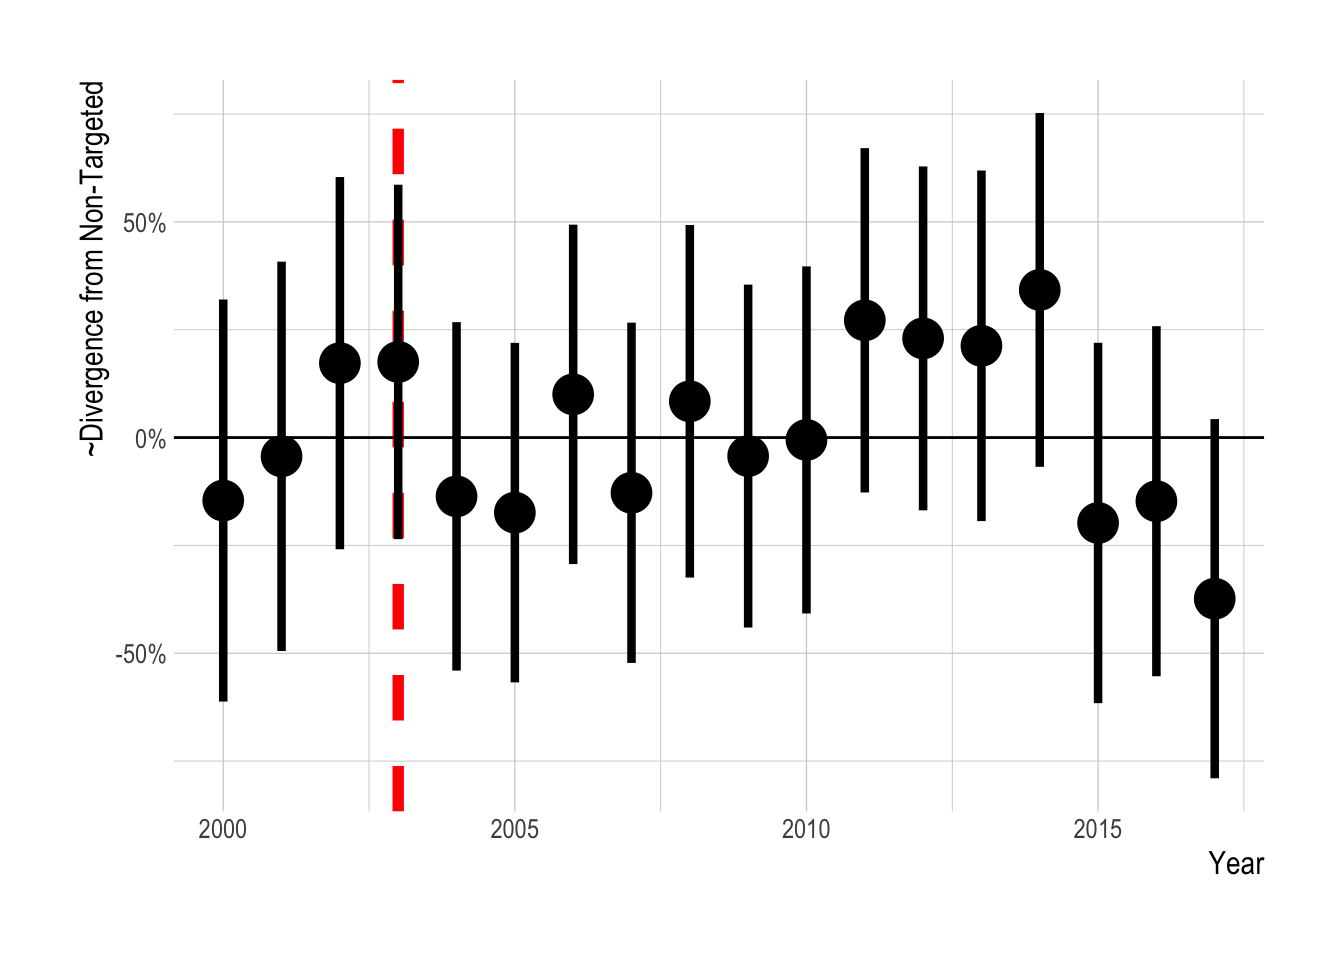
\includegraphics{thesis_files/figure-latex/did-plot-1.pdf}
\caption{\label{fig:did-plot}Estimated divergence in densities of targeted
and non-targeted fishes throughout the Channel Islands (i.e.~integrated
across both inside and outside of MPAs). MPAs are implemented in 2003
(red dashsed line). Estimates are from a regression on log(abundance
index), so estimated effects roughly correspond to percentage changes}
\end{figure}
As a robustness check to these results, we repeated our analysis
utilizing data provided by the
\href{https://science.nature.nps.gov/im/units/medn/monitor/kelpforest.cfm}{Kelp
Forest Monitoring Program (KFM)} conducted in the Channel Islands.
Despite have similar but different methods and survey locations, we find
almost identical estimated trends in divergences between targeted and
non-targeted species using the KFM data (Fig.\ref{fig:kfm-did}).
\begin{figure}
\centering
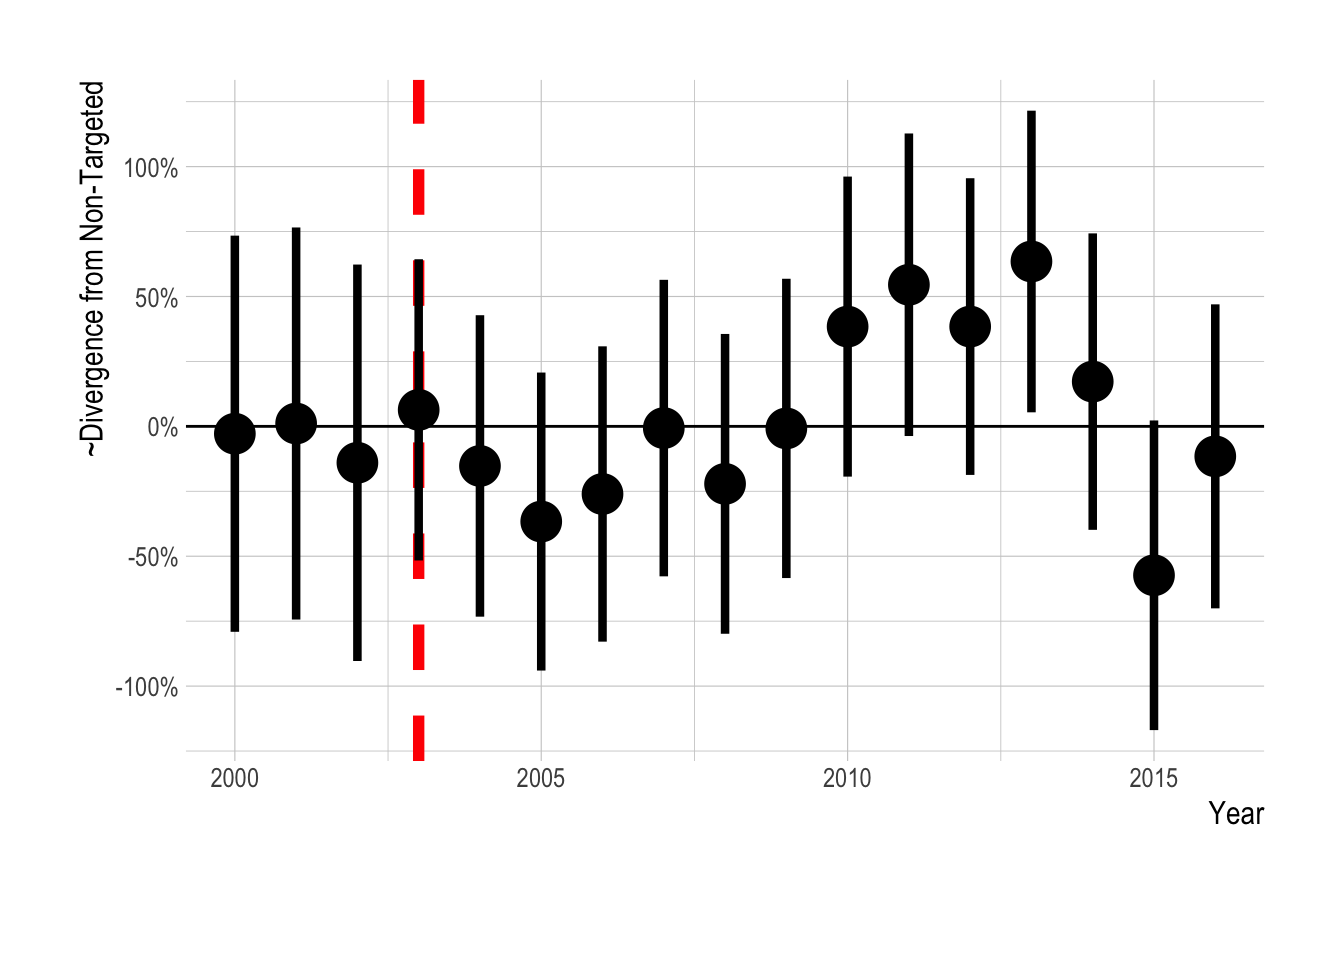
\includegraphics{thesis_files/figure-latex/kfm-did-1.pdf}
\caption{\label{fig:kfm-did}Estimated divergence in densities of targeted
and non-targeted fishes in the Channel Islands (i.e.~integrated across
both inside and outside of MPAs) using the KFM data . MPAs are
implemented in 2003 (red dashed line). Estimates are from a regression
on log(abundance index), and so estimated effects roughly correspond to
percentage changes}
\end{figure}
\subsubsection{Regional Inside vs Outside MPA
Effects}\label{regional-inside-vs-outside-mpa-effects}

Given trends in mean densities observed in Fig.\ref{fig:raw-trend}, the
``regional conservation effect'' estimated by our model, defined as the
divergence in trends between the targeted and non-targeted species
across the Channel Islands region, is not surprising; By jumping through
countless statistical hoops we reach a similar conclusion that we would
just by looking at the divergences in the mean trends. The integration
of data from inside and outside of MPAs is a possible explanation for
this lack of a clear regional effect. If spillover is limited or has
simply not developed yet, especially relative to the effect of fishing
outside of MPAs, then it is possible that there is a clear positive
effect inside the MPAs, a clear negative effect outside, and when we
look across both types of sites we get an unclear average of the two.

To address this, we can first repeat some exploratory data analysis of
trends in densities inside and outside the MPAs for targeted and
non-targeted species. Caselle \emph{et al.}
(\protect\hyperlink{ref-Caselle2015}{2015}) provides a thorough look at
this question of differences inside and outside of MPAs, we update the
analysis here to account for our specific questions of trend divergence,
potential differences in filtering methods, to include data up through
2017, and to utilize our estimation method on just the inside-MPA data.
For all exploratory analyses, we consider the same top 23 consistently
observed species. Looking first at simple trends in total mean biomass
density across these species inside and outside of MPAs, we find
evidence that biomass densities inside the MPAs is increasing faster
(and is higher inside) than outside (Fig.\ref{fig:bio-mpa}).
\begin{figure}
\centering
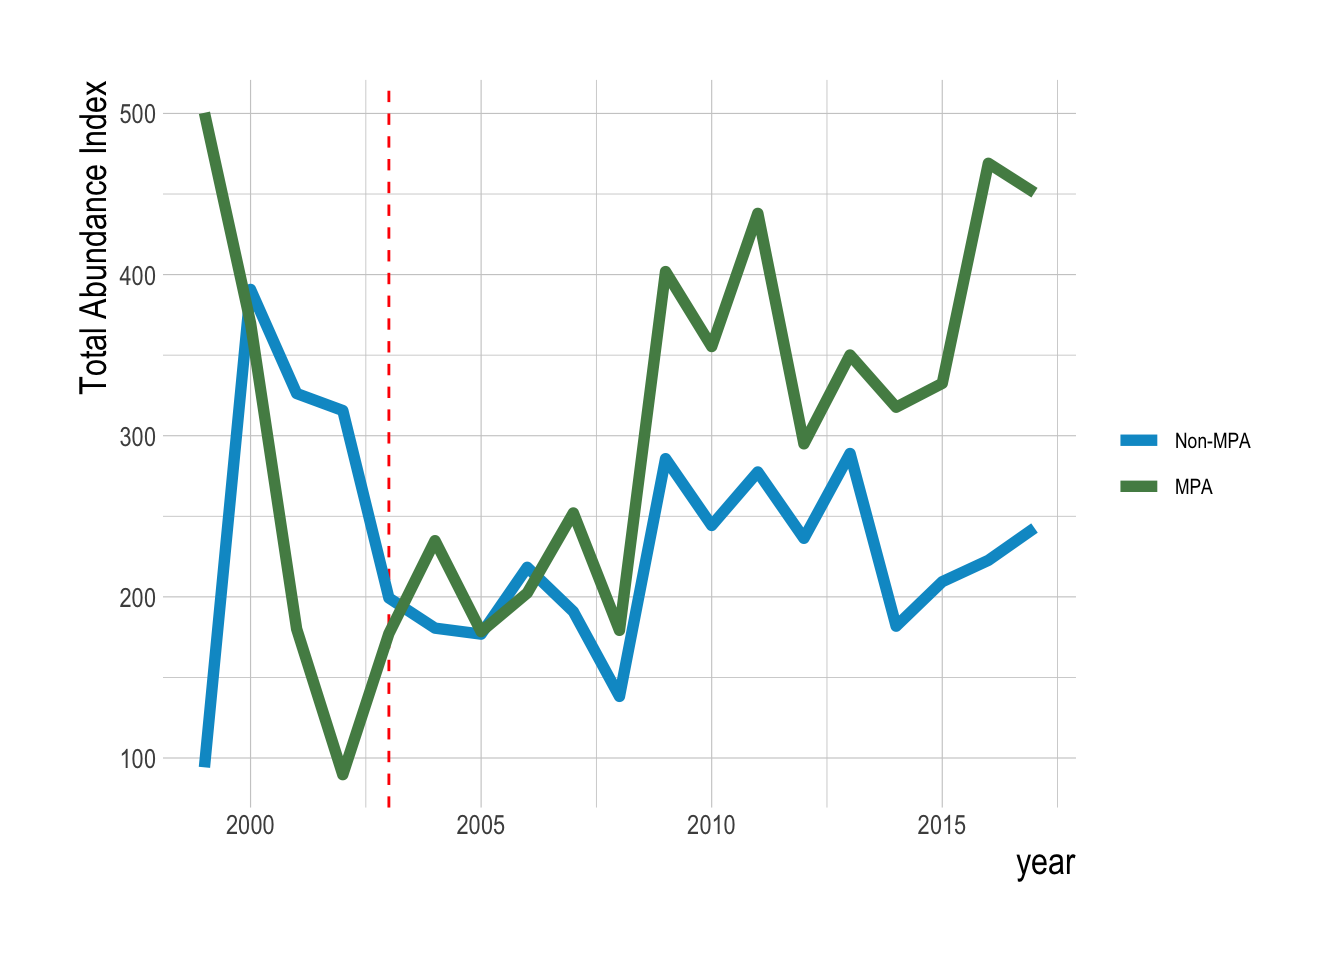
\includegraphics{thesis_files/figure-latex/bio-mpa-1.pdf}
\caption{\label{fig:bio-mpa}Mean aggregate biomass density (summed across
all fishes) inside and outside of eventual MPA locations over time. Red
dashed line indicates MPA implementation year}
\end{figure}
Our proposed identification strategy here though is not that total
biomass density should be different inside and outside, but that the
non-targeted species should serve as the control to the targeted. If we
believe that the MPA effects are greater inside the MPA, then we would
expect to see stronger divergences in biomass densities between these
two targeted and non-targeted fishes inside the MPAs than outside
\begin{figure}
\centering
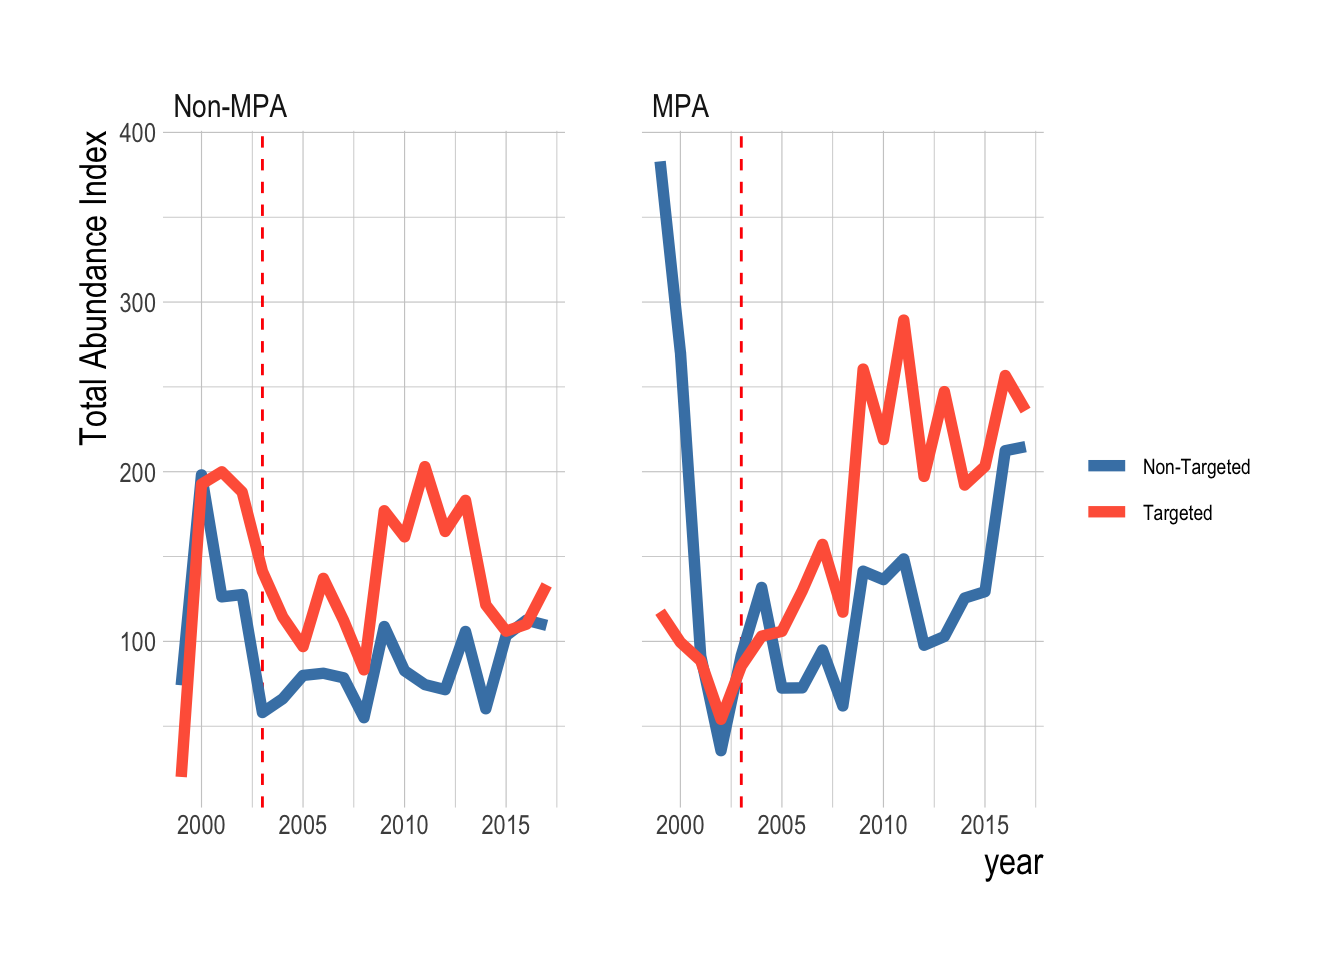
\includegraphics{thesis_files/figure-latex/div-mpa-1.pdf}
\caption{\label{fig:div-mpa}Trends in total biomass density inside and
outside of eventual MPAs for targeted and non-targeted fishes. Red
dashed line indicates MPA implementation year}
\end{figure}
Here we see a different picture. While there is some visual evidence
that the targeted species were diverging from the non-targeted faster
inside the MPAs than outside, both inside and outside we see that the
trend in total biomass density of targeted species is trending downward,
relative to the trend in the non-targeted species in recent years. This
analysis is of total biomass density However, our model estimates the
mean difference in targeted and non-targeted species. Both have their
advantages, but we chose the mean to reflect a hypothesis that the MPAs
would provide positive benefits across all targeted species. The total
biomass density could be strongly affected by a sharp increase or
decrease in one or two species, even if the mean trend is different.
Examining the mean trends though, we see the same results
(Fig.\ref{fig:mean-div-mpa}).
\begin{figure}
\centering
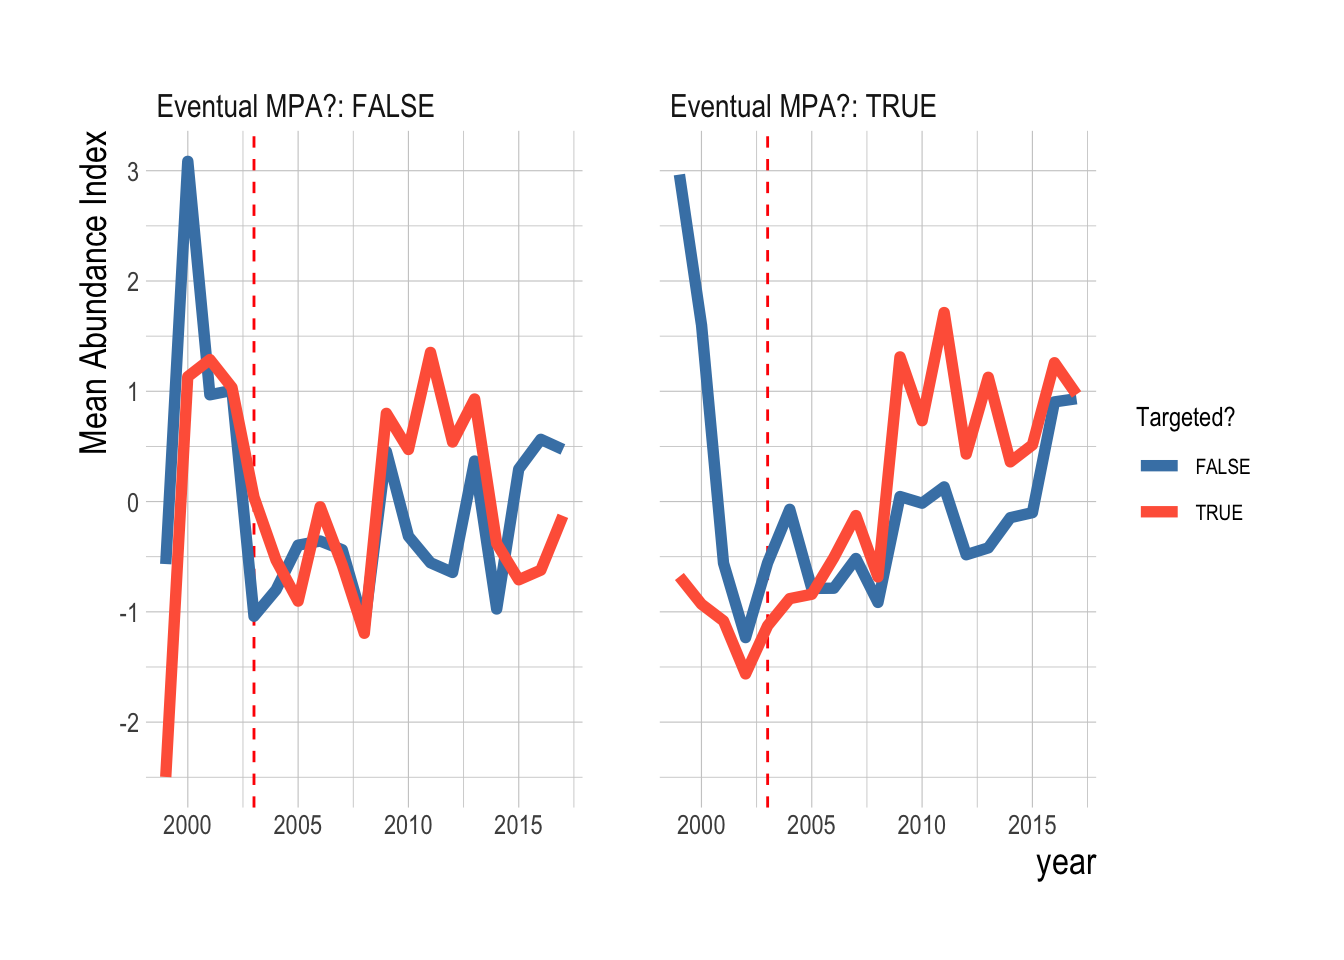
\includegraphics{thesis_files/figure-latex/mean-div-mpa-1.pdf}
\caption{\label{fig:mean-div-mpa}Trends in mean total biomass density inside
and outside of eventual MPAs for targeted and non-targeted fishes. Red
dashed line indicates MPA implementation year}
\end{figure}
Lastly, we can examine both the mean and individual trend to check clear
species-by-species outliers in the overall biomass density trends. This
analysis shows noise, but overall the targeted and non-targeted species
seem to be following similar trends within their respective groups
\begin{figure}
\centering
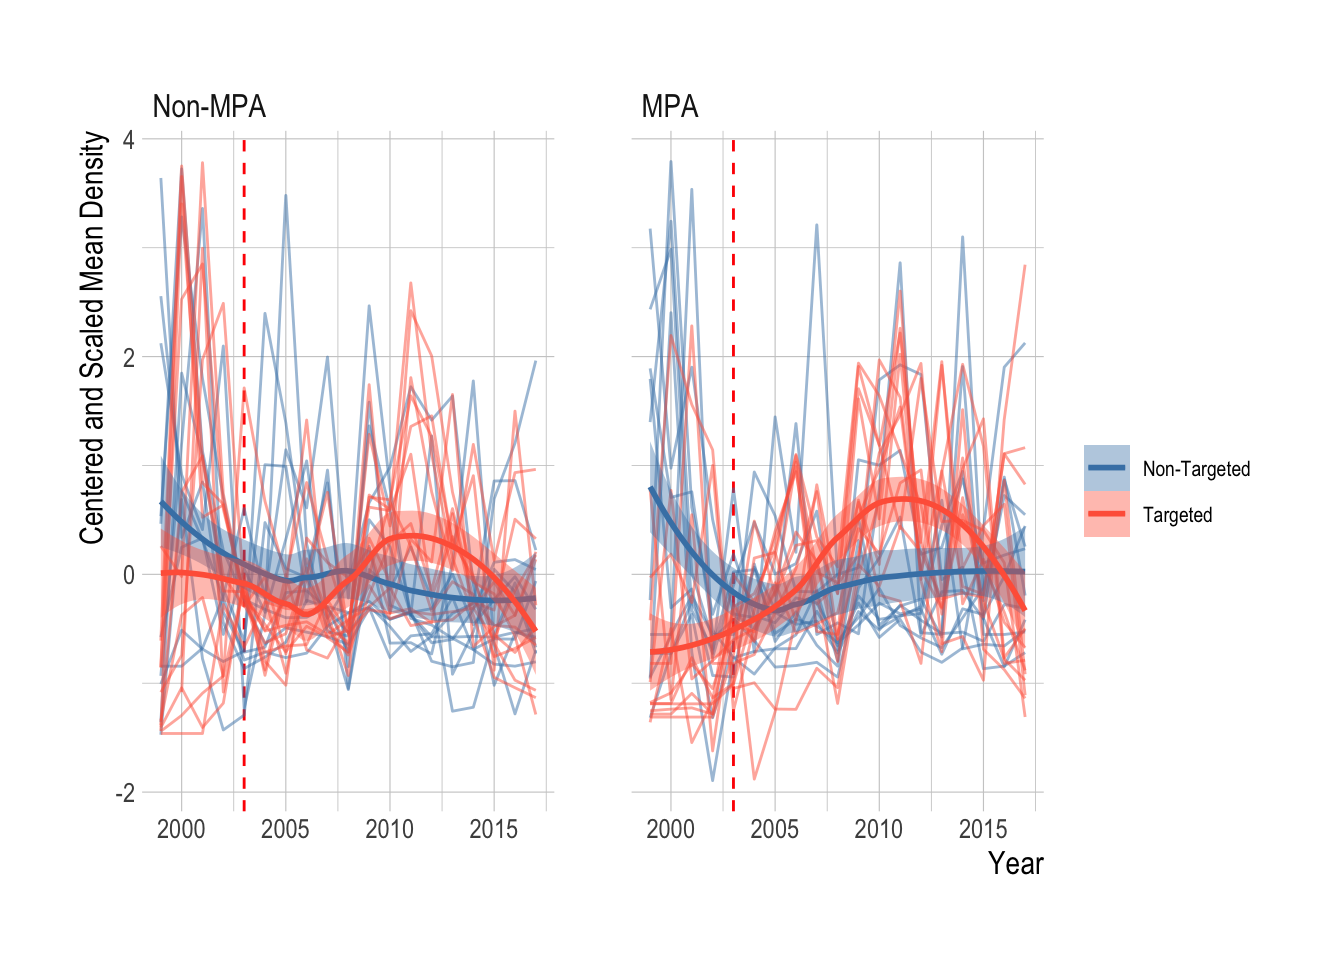
\includegraphics{thesis_files/figure-latex/cs-trends-1.pdf}
\caption{\label{fig:cs-trends}Centered and scaled biomass density trends for
each fish grouped by targeted and non targeted (pale lines) and fitted
LOESS smoother (with 95\% confidence intervals around mean) and mean by
targeted and non-targeted groups, inside and outside od MPAs. Red dashed
line indicates MPA implementation year}
\end{figure}
These visual assessments suggest that similar to our results looking
both inside and outside of MPAs, we would expect that our estimation
model fitted only on data from inside eventual MPAs would reach similar
conclusions as our results fitted to data from both inside and outside
MPAs. To test this, we re-ran our analysis, but only using data from
sites that are eventually placed inside MPAs. Our results reflect the
same trends as displayed in the raw data and the statistical region-wide
analysis, providing robust statistical support to the conclusions we
would reach from visually examining the raw data (Fig.
\ref{fig:mpa-did}).
\begin{figure}
\centering
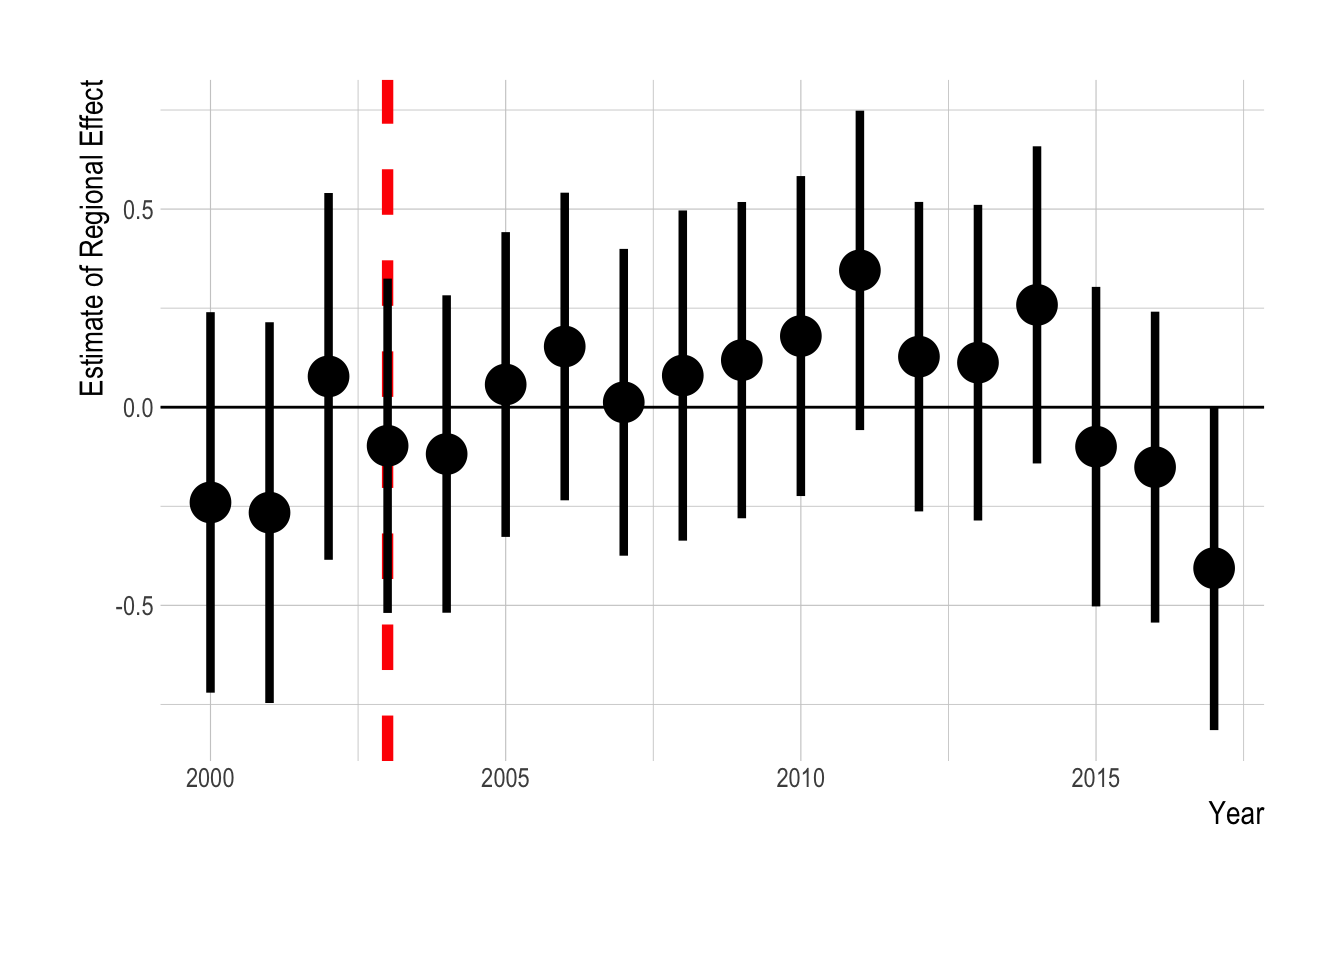
\includegraphics{thesis_files/figure-latex/mpa-did-1.pdf}
\caption{\label{fig:mpa-did}Estimated divergence in biomass densities of
targeted and non-targeted fishes inside eventual Channel Islands MPAs.
MPAs are implement in 2003 (red dashsed line). Estimates are from a
regression on log(abundance index), and so estimated effects roughly
correspond to percentage changes}
\end{figure}
\subsection{Discussion}\label{discussion-1}

MPAs are playing a growing role in the management of marine resources
around the world. While the primary purpose of MPAs is often to protect
species and habitats within their borders, they are also looked to to
provide spillover benefits to the ecosystems and fisheries surrounding
them. The existence and magnitude of these spillover benefits has been a
source of substantial debate for a some time, with the bulk of the
conversation centered around qualitative or theoretical examinations of
particular drivers of spillover (Hilborn and Walters
\protect\hyperlink{ref-Hilborn1992}{1992}; Gaines \emph{et al.}
\protect\hyperlink{ref-Gaines2003}{2003},
\protect\hyperlink{ref-Gaines2010}{2010}; Gerber \emph{et al.}
\protect\hyperlink{ref-Gerber2003}{2003},
\protect\hyperlink{ref-Gerber2005}{2005}; Hastings and Botsford
\protect\hyperlink{ref-Hastings2003}{2003}; Hilborn \emph{et al.}
\protect\hyperlink{ref-Hilborn2004a}{2004}\protect\hyperlink{ref-Hilborn2004a}{a},\protect\hyperlink{ref-Hilborn2004}{b};
Walters and Martell \protect\hyperlink{ref-Walters2004}{2004}; Botsford
\emph{et al.} \protect\hyperlink{ref-Botsford2008}{2008}), or in
detecting empirical evidence of the existence of spillover (Russ and
Alcala \protect\hyperlink{ref-Russ1996}{1996}; e.g. Halpern \emph{et
al.} \protect\hyperlink{ref-Halpern2009}{2009}), but not the net
regional effects of MPAs. As many of the MPA networks around the world
become mature enough for analysis, it is critical that we take a step to
consider what evidence we can expect to observe, and what we have in
fact seen in natural systems.

While a large body of literature has discussed the factors affecting the
regional-scale conservation outcomes of MPAs, we know of no other study
that has synthesized much of the key theoretical predictions of the
literature into a comprehensive simulation framework to address the
cumulative impact of these drivers on the regional effects of MPAs. Our
results present several important insights for understanding what we
might expect the effects of MPAs outside their borders to be. First, we
see that incorporating a broad, but still limited, set of life history,
MPA, and fishery characteristics produces a vast array of potential
regional conservation effects, from actual net conservation losses (in
cases for example of short-term constant-catch, moderate pre-MPA
depletion, and smaller MPA sizes), to massive conservation and fishery
gains (e.g large MPAs in a very depleted fishery). These wide ranges of
outcomes persisted even in extreme cases; small effects were possible in
very depleted fisheries, and larger effects were possible in cases of
moderate depletion. One important result of this analysis is that
looking across the range of ``smaller'' MPAs (covering 25\% or less of
the region), the median regional effect size was relatively small, both
in percentage gains relative to the without-MPA scenario, and in
percentage of unfished biomass recovered, up until the fishery was
strongly depleted
(Fig.\ref{fig:f-and-s-plot}-\ref{fig:pop-f-and-s-plot}).

This has important implications for our ability to empirically detect
these effects in natural systems. Marine environments are complex and
noisy systems, subject to both large amounts of natural variation and
measurement error. Our simulation results suggest then that it will be
relatively difficult to detect the regional-scale effects of MPAs in
many cases of smaller MPAs and moderately depleted fisheries; separating
out say the median simulated population effect of a 0.0035711\% of
unfished biomass is a difficult task even in a carefully studied
environment. With that in mind then, we should not be surprised that our
analysis was unable to determine a clear regional divergence between the
densities of targeted and non-targeted species throughout the Channel
Islands in the 15 years since the newest set of MPAs were implemented in
that region.

What can we infer about the regional effects of the Channel Island MPAs
based on the available data and our analysis? At the simplest level, we
cannot detect a significant divergence in densities of targeted and
non-targeted fishes over the 15 years since the implementation of MPAs
in the Channel Islands. However, it is important to note that we also
cannot say that there has been no divergence. The 95\% confidence
intervals surrounding our year-to-year estimates of the divergences have
a mean range of 1, and cross zero in nearly every year (indicating that
both positive and negative divergences have support from the data).
Since the regression model is a log-linear model (predicting log density
indices), we can interpret the the ``divergence'' coefficients roughly
as percentage differences in the densities of targeted and non-targeted.
The upper end of of our estimated confidence intervals corresponds to a
roughly 50\% increase in densities of targeted species relative to
non-targeted, while at the lower end a 50\% decrease is possible. Within
these ranges though, the mean effect size was 1\%, which corresponds
closely with the median MPA effects predicted by our simulation analysis
for moderately exploited species protected by a reserve network covering
\textasciitilde{}25\% of the region's area.

Do these estimated divergences represent the regional effect of the
MPAs? There are clear reasons why we might think not: differences in
responses to environmental drivers such as El Niño between targeted and
non-targeted species, as well as non-MPA related fishery changes, are
both plausible and capable of distorting our results. Trophic
interactions could also positively (if increases in targeted predators
drive down densities of herbivorous non-targeted species for example) or
negatively (if MPA mediated trophic cascades result in increases in both
targeted and non-targeted densities) bias our results. However, while
these concerns are important, they are not sufficient cause to dismiss
our strategy for estimating the regional conservation effects of MPAs
outright.

First, the assumptions of our identification strategy and operating
models (e.g.~no trophic interactions) reflect the underlying assumptions
of much of the theoretical and simulation based literature on MPA
effects used to motivate much of modern MPA design (Gaines \emph{et al.}
\protect\hyperlink{ref-Gaines2010}{2010}; and fisheries management more
broadly, Fulton \emph{et al.} \protect\hyperlink{ref-Fulton2015}{2015}).
This of course does not mean that these assumptions are correct, but
dismissing our results purely on the basis of for example the potential
for trophic interactions requires then that we also rethink much of the
work on which MPA design is based (we can't use single species models to
predict MPA effects but dismiss a single species model to estimate their
effect). All else being equal, most standard models of MPA effects would
predict faster and more substantial changes in densities of targeted
fishes post MPA implementation than for non-targeted species, which is
exactly what our model is designed to detect. If trophic feedbacks in
the form of decreases in non-targeted prey as targeted predators rebound
do exist, this would actually serve to positively bias our estimate of
regional conservation MPA effects. Our cross-mapping analysis does not
suggest that trophic interactions are playing a substantial role in our
results.

Second, our identification strategy is an improvement over the
alternatives that are likely to be available in most cases. We could
simply compare regional densities of fish before and after MPA
implementation. Doing so in the case of the Channel Islands suggests
that, controlling for observable covariates, densities of targeted
species have declined substantially post-MPA
{[}Fig.\ref{fig:obs-plot}{]}. The reason we are skeptical of this
conclusion though is of course that other non-MPA factors for which we
do not have adequate data to include in the model could be driving that
decline. The relatively parallel pre-MPA trends in densities of targeted
and non-targeted species suggests that this is indeed the case. We would
of course prefer some form of control group rather than simply
before-after comparisons. However, for all but the most specialized of
cases we are unlikely to ever have effective spatio-temporal controls
for MPAs (e.g.~an MPA-less carbon-copy of the Channel Islands, though
see ({\textbf{???}}) for an example of using different regions as
attempted controls). Given these constraints then, measuring the
regional divergence in targeted and non-targeted species is likely to be
among the best available options for empirically estimating the
region-wide conservation effects of MPAs given the kinds of data that
are often collected in conjunction with MPAs (transect surveys inside
and outside of reserves).

Along with the identification strategy, there are clear fundamental
challenges to accurately estimating densities of different species
across a large marine region. Dive conditions can greatly impact the
ability of divers to make accurate counts. Density estimates of highly
mobile species can be positively biased {[}Ward-Paige2010{]}. Funding
constraints limit the ability to consistently monitor all important
sites throughout a region. This analysis also only considers finfish;
invertebrate targeted species such as urchin and lobster that often have
small home ranges in their adult stages may demonstrate clearer MPA
effects (e.g. Kay \emph{et al.} \protect\hyperlink{ref-Kay2012}{2012}).

One potential alternative to a regression-based identification strategy
would be structural modeling of MPAs within a stock assessment process
(Field \emph{et al.} \protect\hyperlink{ref-Field2006}{2006}).
Conditional on having high quality data, the key problem in the
regression based approach we present here is isolating MPA spillover
effects, fleet responses, and environmental shocks from each other.
Integrated stock assessments (as described in Hilborn and Walters
\protect\hyperlink{ref-Hilborn1992}{1992}) provide a potential way to
estimate these effects. The ability of larval spillover to provide
conservation gains assumes a relationship between spawning stock biomass
and recruitment. Therefore, within a stock assessment the relative
importance of estimated recruitment deviates to estimated population
trajectories could provide an index of how much increases in spawning
stock biomass resulting from an MPA are contributing to recruitment vs
the effect of environmental drivers. Similarly, spatial estimates of
fishing mortality and biomass can help answer whether total mortality
and biomass have gone up or down following MPA implementation. Such an
analysis though would require integrating data from inside and outside
of MPAs (which fishery dependent data cannot do) and research programs
such as PISCO provide a natural platform for this type of analysis to
build off of.

Our estimated regional divergences in the densities of targeted and
non-targeted fishes present an imperfect but improved (relative to
alternative options) window into the regional effects of the Channel
Islands MPAs. Our results leverage the evidence of parallel trends
between the targeted and non-targeted fishes to refute the conclusion of
post-MPA declines in densities we would reach if we simply looked at
pre-and-post MPA densities of targeted species. But, we also do not find
clear evidence for substantial increases in densities of targeted
species, relative to the trend we would expect given the densities of
the non-targeted species. We do see some evidence for an increasing
trend in targeted densities from 2003 to 2014, but this period is
followed by signs of decreases from 2015 onward. The magnitude and
direction of both of these changes are plausible effects of MPAs,
according to our simulation analysis. The early upward trend could
certainly be attributable to larval or adult spillover from the MPAs, as
well as biomass buildup inside the MPAs themselves. The later decline
could be due to concentrated fishing pressure outside the reserves.

It is also possible though that factors exogenous to the MPAs themselves
are driving the apparent recent decline in the trends of targeted
species relative to the non-targeted. For example, an increase in
fishing effort resulting from market forces could explain the recent
downturn, but we would not want to attribute that as a regional
conservation effect of the MPAs themselves (though including estimates
of commercial landings for species in our analysis did not change our
results, suggesting that this downtown cannot be explained by total
catch alone). The presence of a downward trend in the estimated regional
when we look just inside the MPAs suggests that environmental drivers
may be the culprit here. If we assume that the MPAs are indeed well
enforced and large enough to provide some substantial protection from
fishing for at least some of the targeted species, which we have every
reason to believe (Caselle \emph{et al.}
\protect\hyperlink{ref-Caselle2015}{2015}), then if the cause of the
recent downturn estimated by our model were increased fishing, we would
expect to see that effect masked or at least dampened in the within-MPA
data and analysis. That we still see the decline in the within-MPA data
provides evidence that a broader environmental event is depressing the
trend in the targeted species, such as the large El Niño events of
2009-10 and 2014-2016. This is supported by the clear warming signal in
measured sea surface temperatures throughout the Channel Islands in
recent years (Fig.\ref{fig:temp-plot}). While our simulation analysis
focused on the structural characteristics of a fishery system that could
make it more or less able to provide regional scale conservation
benefits, these results highlight the critical importance of
environmental drivers in the actual year-to-year effects of marine
conservation policy.
\begin{figure}
\centering
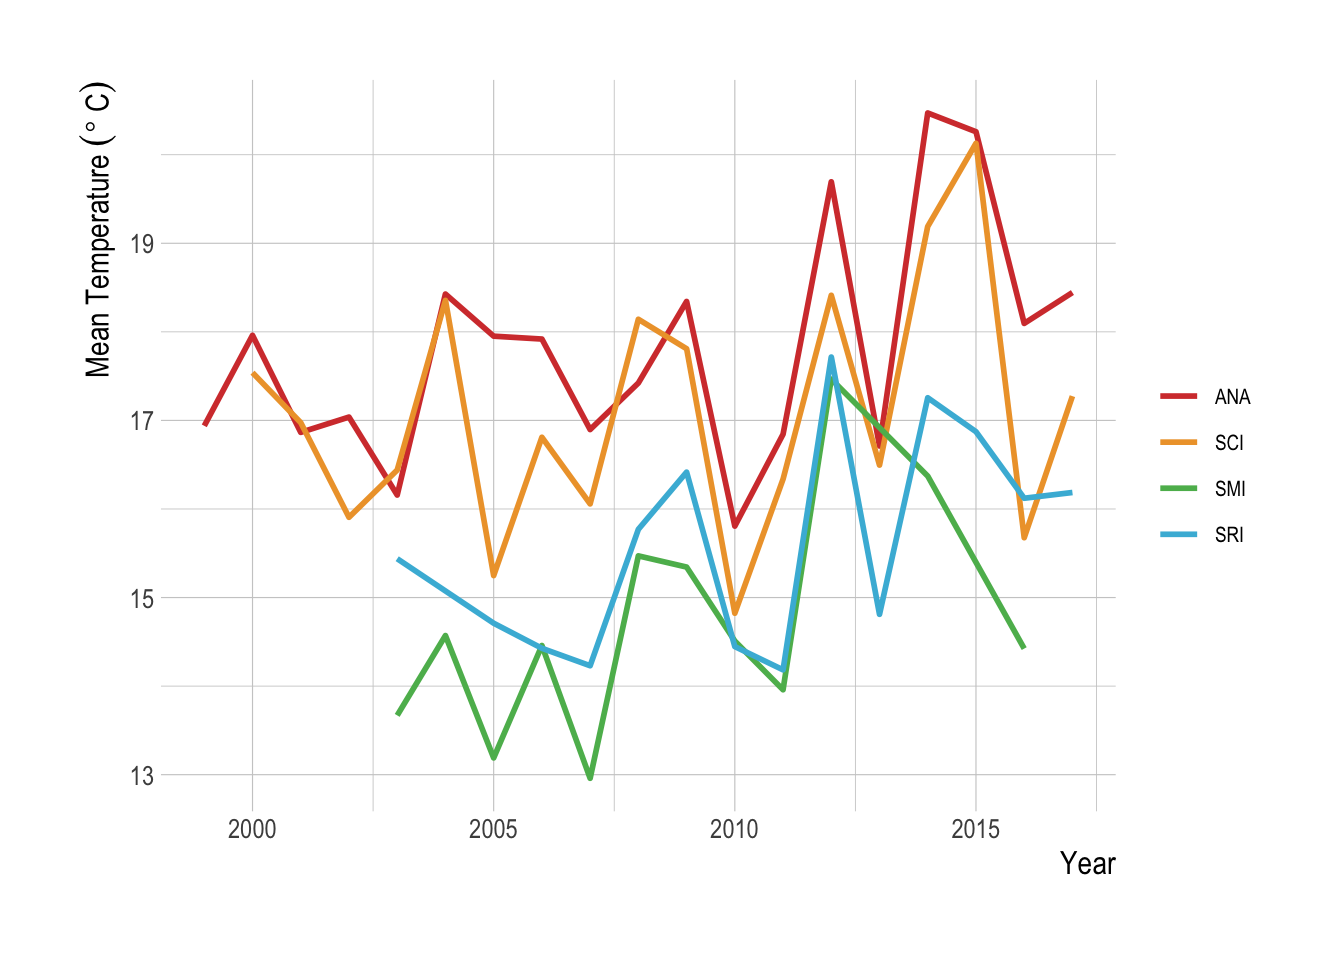
\includegraphics{thesis_files/figure-latex/temp-plot-1.pdf}
\caption{\label{fig:temp-plot}Mean temperature over time at each of the
Channel Islands included in this study}
\end{figure}
Despite the vast amount of rigorous data collection before and after,
our identification strategy was unable to identify a clear signal of the
effect of MPAs on the regional densities of targeted species. Our
simulation analysis indicates though that we should not be surprised by
this. The Channel Islands MPAs cover approximately 21\% of the waters in
the Channel Islands, and while formal stock assessments are not
available for many of the targeted species in our analysis what evidence
we have does not suggest they as a group they are heavily overfished.
Our simulation analysis would suggest then that the percentage
difference in densities of targeted species with and without MPAs should
be on the smaller end (10\% or less), and therefore be challenging to
detect given the natural variation of marine ecosystems and the error
inherent in visual survey programs such as those the PISCO data used
here. What then does this suggest for the design and monitoring of MPAs?

Real world-policy making is inherently an exercise in utilizing best
available theory, experience, and modeling to make decisions that are
often difficult or practically impossible to empirically test. Despite
our best efforts we are unlikely to ever truly ``know'' the effect of
our efforts to mitigate climate change, but must instead rely on
comparisons to best available modeling outcomes to understand how
effective our policies have been. Similarly, given the complexities of
marine systems much of our decisions on MPA design will have to be based
on effective modeling. While we are hardly the first to point out that
bio-economic models are a critical tool for MPA design, our results help
indicate a minimum floor of model complexity to provide candid
assessments of regional MPA effects. While factors such as MPA size and
degree of depletion are especially strong drivers, for all but the most
extreme cases of each a wide array of effects, from negative to highly
positive, are possible based on the complex interaction of factors such
as fleet dynamics, movement rates, and recruitment timing. Confronting
these interactions by considering the likely parameter space for a given
region is a critical step then in understanding what likely regional
effects of MPAs are. While models such as ours do require large numbers
of parameters that may be challenging to obtain, our results show that
working with communities to confront these uncertainties is preferable
to sweeping them under the rug in favor of simpler models that are
easier to parameterize but miss details that our results show can have
dramatic effect on expected outcomes. Modeling effort such as this can
then provide stakeholders with some idea of the range of regional effect
sizes that might be expected for a given MPA network design, and in
doing so design monitoring programs targeted at the species and fleets
that modeling suggests may provide the clearest indication of MPA
mediated effects. For cases where bio-economic modeling suggests small
potential for MPA driven regional density effects, monitoring efforts
can be targeted around detecting potential negative effects should they
arise, i.e.~evidence that the model is wrong, rather than exerting
massive amounts of effort on what theory and modeling suggest may be a
small effect size.

We focus mostly on regional conservation gains in this paper. However,
fisheries spillover is often another important factor to consider
(i.e.~are fisheries better off with the MPAs than they would have been
without them). The fishery benefits of MPAs are just as (and likely
more) intensely debated than the regional conservation outcomes (Roberts
\emph{et al.} \protect\hyperlink{ref-Roberts2001}{2001}; Hilborn
\emph{et al.}
\protect\hyperlink{ref-Hilborn2004}{2004}\protect\hyperlink{ref-Hilborn2004}{b};
Hilborn \protect\hyperlink{ref-Hilborn2018}{2018}; Sala and Giakoumi
\protect\hyperlink{ref-Sala2018b}{2018}). We only address fisheries
affects briefly in this study, but our results highlight important
tradeoffs and synergies between conservation and fishery spillover
effects of MPAs. The good news from a fisheries perspective is also
fairly obvious: Both the regional conservation and fishery benefits are
expected to be greatest when the fished population is in an extremely
depleted state pre-MPA, even over a 15 year time horizon, even for
larger MPAs (though further work is needed to compare MPAs to
alternative fisheries management strategies in these cases). For cases
where a valuable and formerly abundant species is overfished, a large
MPA may then provide large conservation and fishery gains for that
species, while potentially having smaller impacts on other less depleted
species. Our simulation results also do identify though a large
parameter space where MPAs create tradeoffs between moderate
conservation gains and moderate fishing losses. This type of projection
analysis can help managers consider where in this space they may be. The
most critical point with regards to conservation and fishery effects
from our simulation analysis is that the conservation or fishery effects
of MPAs cannot be reliably estimated without some knowledge and
consideration of the dynamics of the fishing fleet outside the MPAs:
over the short-term open access vs constant catch dynamics can make the
difference between a substantial conservation and fisheries win to a
more depleted stock with more expensive fishing.

MPAs are an important part of the marine resource management toolbox.
Under ideal circumstances they can protect both individual species and
ecosystem linkages, safeguard crucial habitat, and support local
economies through tourism and fishing opportunities. However, our
results show that the regional conservation and fishery benefits we
should expect from MPAs are highly variable, and while we cannot assign
probabilities to our simulated states of nature, we find that there are
more opportunities for smaller effect sizes than large, especially in
the short-term. Most importantly, our results highlight the critical
importance of explicitly modeling the links between the biological
effects of MPAs and the ways that humans respond to them. Large-scale
empirical evidence supports our results that accurately predicting the
effects of MPAs depends on understanding the human context in which they
find themselves (Cinner \emph{et al.}
\protect\hyperlink{ref-Cinner2018}{2018}). While this is far from the
first effort at simulating MPAs, our model fills an important niche
between more focused theoretical models that address a few drivers of
MPA performance at a time but do not address complicated linkages
between drivers, and more site-specific models that provide best
available local results but are challenging to scale to different
systems. This intermediate complexity model allows us to simulate tens
of thousands of fisheries containing most of the key drivers of MPA
performance identified by theory.

This process provides a unique survey of the likely regional effects of
MPAs to fisheries and conservation, and places our empirical assessment
of the regional effects of the Channel Islands MPAs in context. The
Channel Islands are an intensely studied system, and the challenge of
identifying a clear regional effect of the network of MPAs placed there
in 2003 may seem surprising. However, our results show that in fact a
smaller effect size, from the perspective of regional conservation
gains, is to be expected in this system, and therefore the true effect
will be very challenging to separate from environmental noise. The
solution then though is not to give up on detecting effects, but rather
to shift focus from identifying a specific effect size and instead use
simulation analysis to appropriately set expectations for conservation
and fishing stakeholders, and design monitoring programs around the
species and situations that serve as effective indicators of the ability
of an MPA network to achieve its objectives.

\section{Methods}\label{methods-2}

\subsection{Simulation Model}\label{simulation-model}

The simulation model used in this analysis is roughly the same as the
one described in Ovando \emph{et al.}
(\protect\hyperlink{ref-Ovando2016a}{2016}). It is an age structured,
spatially explicit, bio-economic model. Recruitment is assumed to have
Beverton-Holt dynamics on average, though auto-correlated log-normal
recruitment deviates can be specified. The timing of density dependence
can be one of five forms presented in Babcock and MacCall
(\protect\hyperlink{ref-Babcock2011}{2011}), ranging from independent
density dependence in each patch to density dependence in a shared
larval stage across patches. The model allows for both adult and larval
movement, where larval movement is assumed to follow a Gaussian
dispersal kernel based on the distance of each patch to the source
patch. Adult movement is also modeled using a Gaussian dispersal kernel,
but with the added option of density dependent movement as well. In the
adult density dependent movement scenario we calculate the density
gradient between each patch and every other patch, where the density
gradient is calculated as

\[g_{i,j} = \frac{b_i}{b_i^0} - \frac{b_j}{b_j^0} + 1\]

Where \emph{i} is the source patch and \emph{j} is a sink patch, and
\(b^0\) is the unfished biomass in a given patch. The density gradient
\(g_{i,j}\) is used as a multiplicative modifier for the distance-based
Gaussian dispersal kernel \emph{d}, so that the net movement \emph{m} of
individuals from patch \emph{i} to patches 1:J is

\[m_{i,j} = \frac{d_{i,j}g_{i,j}}{\sum_{1:J}d_{i,j}g_{i,j}} \]

Fishing activity is controlled by a fleet model that can take one of
four forms: constant catch, constant effort, and open-access. For the
constant effort and constant catch scenarios, a specified effort or
catch level is set to achieve a target level of pre-MPA depletion, and
that effort or catch is held constant post-MPA. For the open-access
scenario, we model effort through a profit-response function, where
profits are calculated per

\[profits_{t} \sim p_{t}q_{t}E_{t}B^{c}_{t} - c_{t}E_{t}^{\beta}\]

And then effort is modeled as

\[effort_{t} = effort_{t-1} + effort_{msy}(\theta\frac{profits_{t-1}}{profits_{msy}})\]

The operating model allows for time-varying and auto-correlated
deviations in prices \emph{p}, cost \emph{c}, and catchability \emph{q}.
For all fleet model scenarios, effort is distributed in space in one of
two manners: divided equally among all fish-able patches, and
distributed in proportion to historic profits in each patch.

MPAs are implemented in the operating model by setting a specified
percentage of the patches to be placed in a no-take MPA. Patches are
then assigned to an MPA either in a linear fashion (left to right) or
assigned at random throughout the patches. In all scenarios MPAs are
implemented halfway through the simulated time series (allowing the
pre-MPA fishing mortality to deplete the population to a desired level
beforehand).

Using this operating model, we simulated MPA effects across 20,000
fisheries, where the regional effect is modeled by running the exact
same fishery simulation with and without MPAs, and then calculating the
difference in biomass in each year between the two scenarios (setting
identical seeds for each simulation). The range of evaluated scenarios
is presented in Fig.\ref{fig:num-sims} and Fig.\ref{fig:chr-sims}.
\begin{figure}
\centering
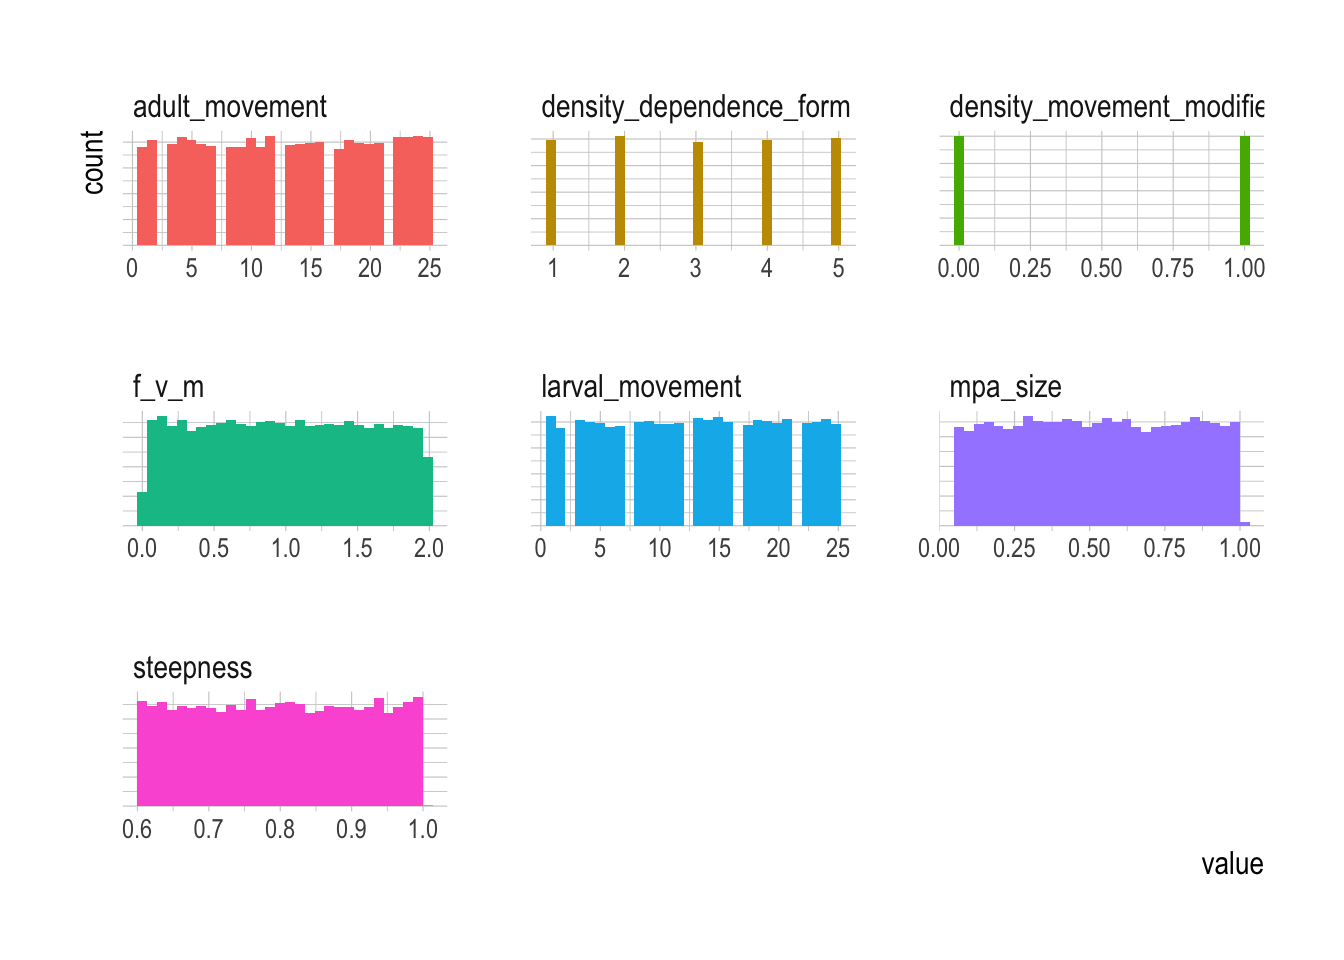
\includegraphics{thesis_files/figure-latex/num-sims-1.pdf}
\caption{\label{fig:num-sims}Histrogram of continuos variable levels across
simulated fisheries}
\end{figure}
\begin{figure}
\centering
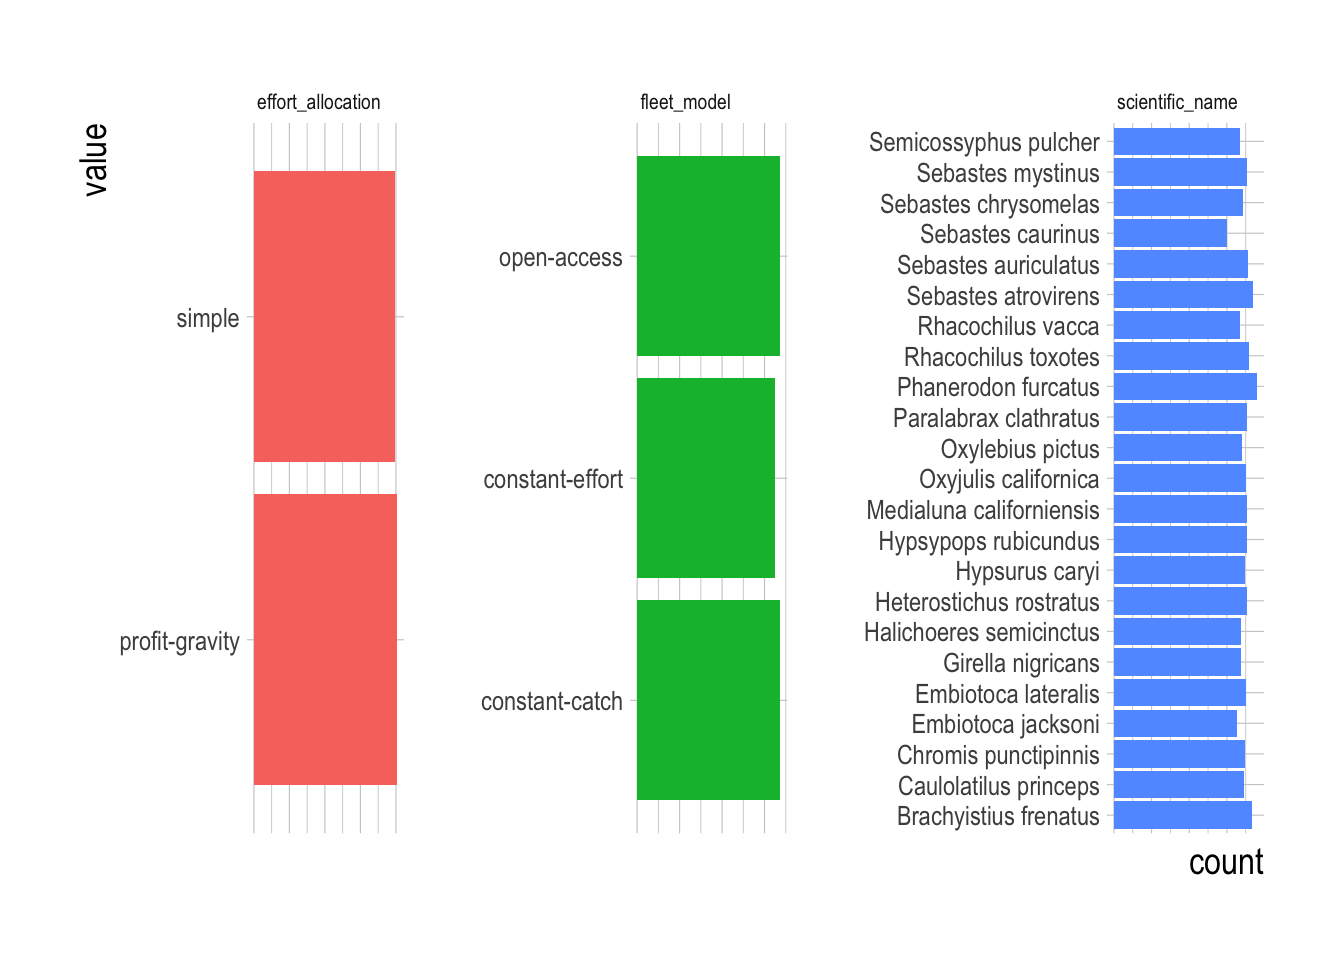
\includegraphics{thesis_files/figure-latex/chr-sims-1.pdf}
\caption{\label{fig:chr-sims}Counts of categorical variable levels across
simulated fisheries}
\end{figure}
\subsection{Regression Analysis}\label{regression-analysis}

The regression analysis uses a mixed-effects hierarchical model. The raw
data are estimated length compositions by fish species along a transect
at a site. Lengths are converted to biomass per allometric relationships
supplied by PISCO and supplemented by the \texttt{FishLife} (Thorson
\emph{et al.} \protect\hyperlink{ref-Thorson2017d}{2017}) package in R
where needed. We performed some minimal data filtering to reduce noise
in the data. We only include species that were observed at least twice
in each year of the dataset (2000-2017) somewhere in the core Channel
Islands (Anacapa, Santa Cruz, Santa Rosa, San Miguel). While some data
are available from 1999, per consultation with PISCO we omit those data
due to changes in survey protocols. We assign species to targeted and
non-targeted groups per the PISCO classifications. This filtering
process results in 11 non-targeted species and 12 targeted species
remaining in the analysis.

The first stage of the regression is a log-normal delta model. The model
estimates two regressions, the first is a binomial generalized linear
model (GLM) with a logit link estimating the probability of observing a
given fish species at a observation \emph{i} (transect at time
\emph{t}). The probability that a given species was observed \emph{o} at
a given observation is distributed

\[o_{s,i} \sim binomial(\frac{1}{1 +e^{-\beta^{o}{X}}}) \] where
\(\beta^{o}\) are the estimated coefficients for the observation model
and \emph{X} is a matrix of covariates that include random effects for
each year in the data (2000 to 2017).

The expected density \emph{d} of positive observations is modeled per a
log-normal distribution

\[log(d_{s,i}) \sim normal(\beta^{d}X, \sigma_s)\]

where \(\beta^{d}\) are the estimated coefficients for the expected
density model and \emph{X} is the same matrix of covariates as used in
the observation portion of the model and \(\sigma_s\) allows for each
species \emph{s} to have different standard deviations.

Our covariate matrix \emph{X} contains both fixed and random effects.
Fixed effects include the depth level of the transect, the sampling
site, the month of the observation, the estimated surge at the transect,
visibility, the depth of the transect, and the experience (and
experience squared) of the diver conducting the transect. We classify
each species into one of two clusters based on the mean longitude the
species was encountered at, breaking the species into two groups: those
primarily found in the western end of the Channel Islands those found
more in the eastern end. We then estimate random effects for each island
for each cluster

\[\beta_{island,cluster} \sim normal(0,\sigma_{cluster})\]

This allows the mean effect of each island to differ for each cluster,
e.g.~allowing the San Miguel, the eastern most island, to have a higher
mean density for eastern species than for more western species (if the
data suggest it).

The second critical component of the covariate matrix \emph{X} are
random effects for each year for each species

\[\beta_{year,species} \sim normal(0,\sigma_{species})\]

These \(\beta_{year,species}\) represent our ``standardized'' estimate
of observed abundance of each species in each time step, controlling for
the included covariates.

However, we still need to account for changes in the probability of
detection over time. For that, we create a standard matrix of with rows
equal to the number of years and columns corresponding to each of the
columns in \emph{X}, holding everything fixed at mean (or most
frequently observed level for factors) levels for all variables in X
except for the year and species interaction indices. Calling this
standardized matrix \(X^{standard}\), the probability of observing a
given species in year \emph{y} is then

\[p_{s,y} = (\frac{1}{1 +e^{-\beta^{o}{X^{standard}}}})\]

In the same manner as described by Punt \emph{et al.}
(\protect\hyperlink{ref-Punt2000}{2000}), The standardized index of
abundance for species \emph{s} in year \emph{y} then is

\[I_{species,year} = p_{species,year}e^{\beta_{species,year}}\]

The next phase of the model requires us to estimate the mean abundance
of targeted and non-targeted species over time. The concept here is that
each \(I_{species,year}\) can be modeled by a regression that contains
random effects for each year for targeted and non-targeted fishes, the
assumption then being that there is a mean density for targeted and
non-target species, and \(I_{species,year}\) represent deviations from
that mean.

\[log(I_{species,year}) \sim normal(\beta^{effect}X^{effect}, \sigma_I)\]

\(X^{effect}\) contains both fixed and random effects. The fixed effects
include an intercept and the temperature deviation for a given species
in a year, where temperature deviation is

\[t_{s,y} = (t^{pref}_{s} -  \bar{t_{y}})^2\]

where \(t^{pref}\) is the preferred temperature for species \emph{s}
(drawn form \texttt{FishLife}, Thorson \emph{et al.}
(\protect\hyperlink{ref-Thorson2017d}{2017})), and \(\bar{t_{y}}\) is
the mean temperature encountered by that species in year \emph{y}. We
also include as variables in the model the mean kelp cover experienced
by a given species in a given year, as well as the total fishery catches
reported in the previous year for that species in the Santa Barbara
region {[}drawn from the California Department of Fish and Wildlife
database{]}. We also include random intercepts for each species in
\(X^{effect}\). The most important random effects are year effects for
targeted and non-targeted species

\[\beta_{year,targeted} \sim normal(0,\sigma_{targeted})\]

\(\beta_{year,targeted}\) is the mean log density of targeted species in
year \emph{y}, controlling for included covariates. Therefore, the final
step in the model, the divergence in the standardized abundance trends
of targeted and non-targeted species is

\[divergence_{year} =  \beta_{year,targeted = 1} - \beta_{year,targeted = 0}\]

The model is fit in TMB to integrate the uncertainty across all levels
of the model, with standard errors for each coefficient in the model
estimated through the Laplace approximation.

Figures \ref{fig:fe-plot}:\ref{fig:targ-plot} present estimated effects
for covariates included in the model, along with the raw estimated mean
trends of the targeted and non-targeted species (while the difference
between these trends is presented in our main results
Fig.\ref{fig:did-plot}).
\begin{figure}
\centering
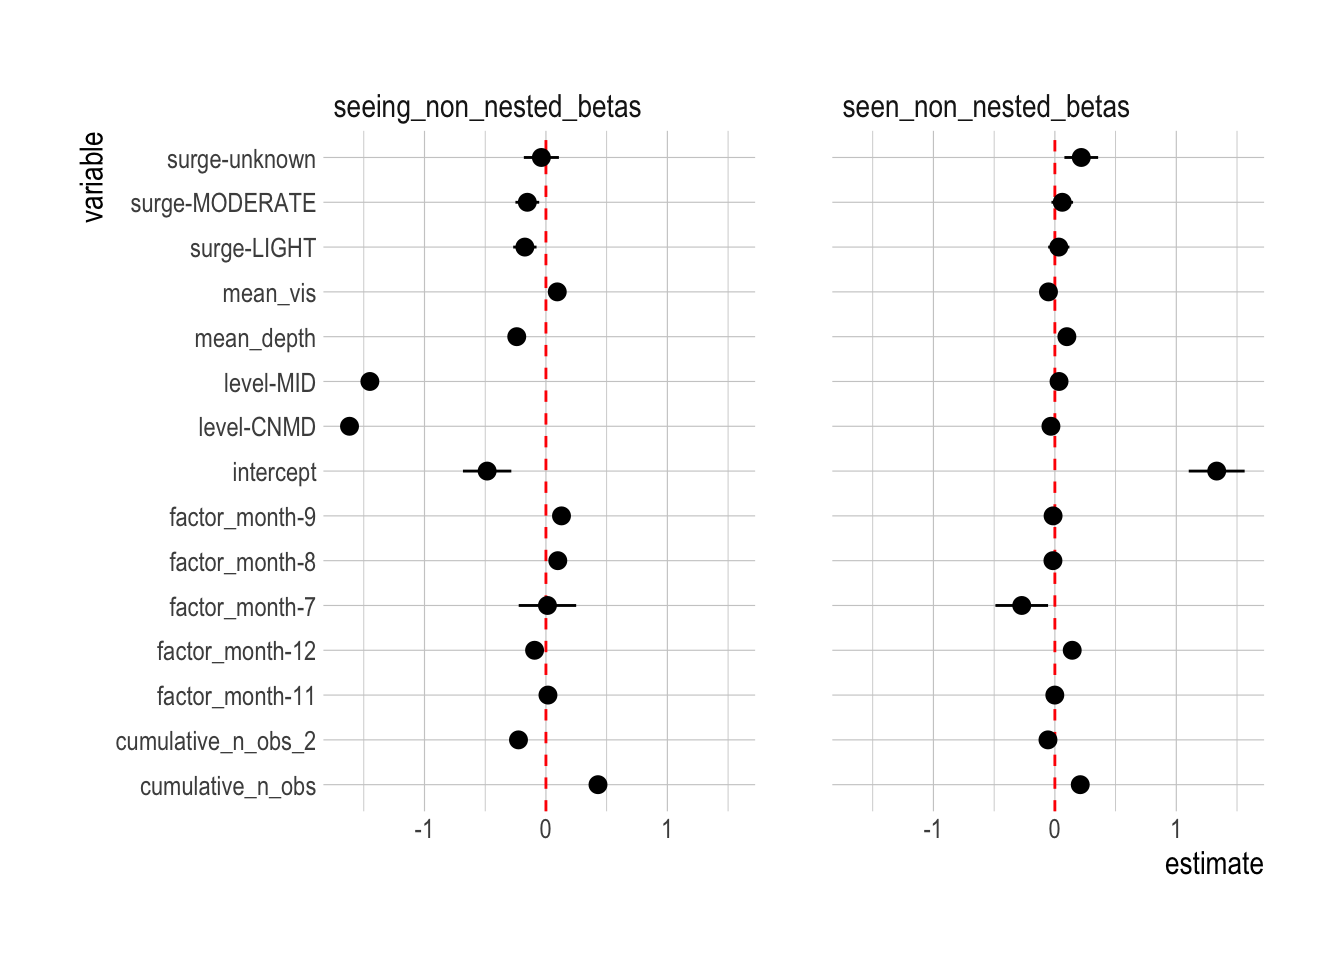
\includegraphics{thesis_files/figure-latex/fe-plot-1.pdf}
\caption{\label{fig:fe-plot}Estimated coefficients for non-spatial fixed
effects in observation model (seeing) and observed model (seen)}
\end{figure}
\begin{figure}
\centering
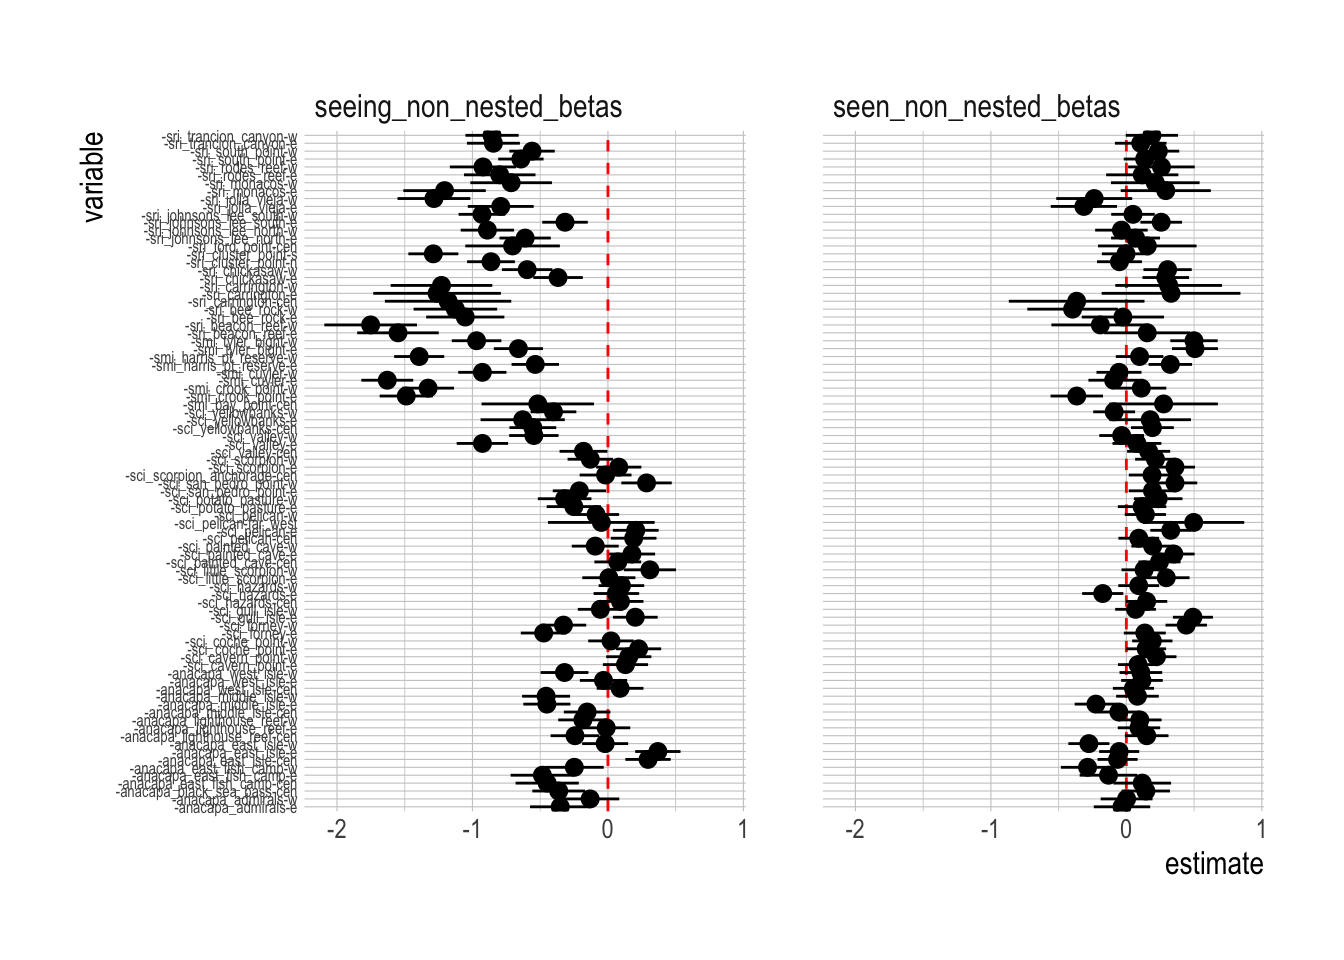
\includegraphics{thesis_files/figure-latex/site-plot-1.pdf}
\caption{\label{fig:site-plot}Estimated coefficients for spatial random
effects in observation model (seeing) and observed model (seen)}
\end{figure}
\begin{figure}
\centering
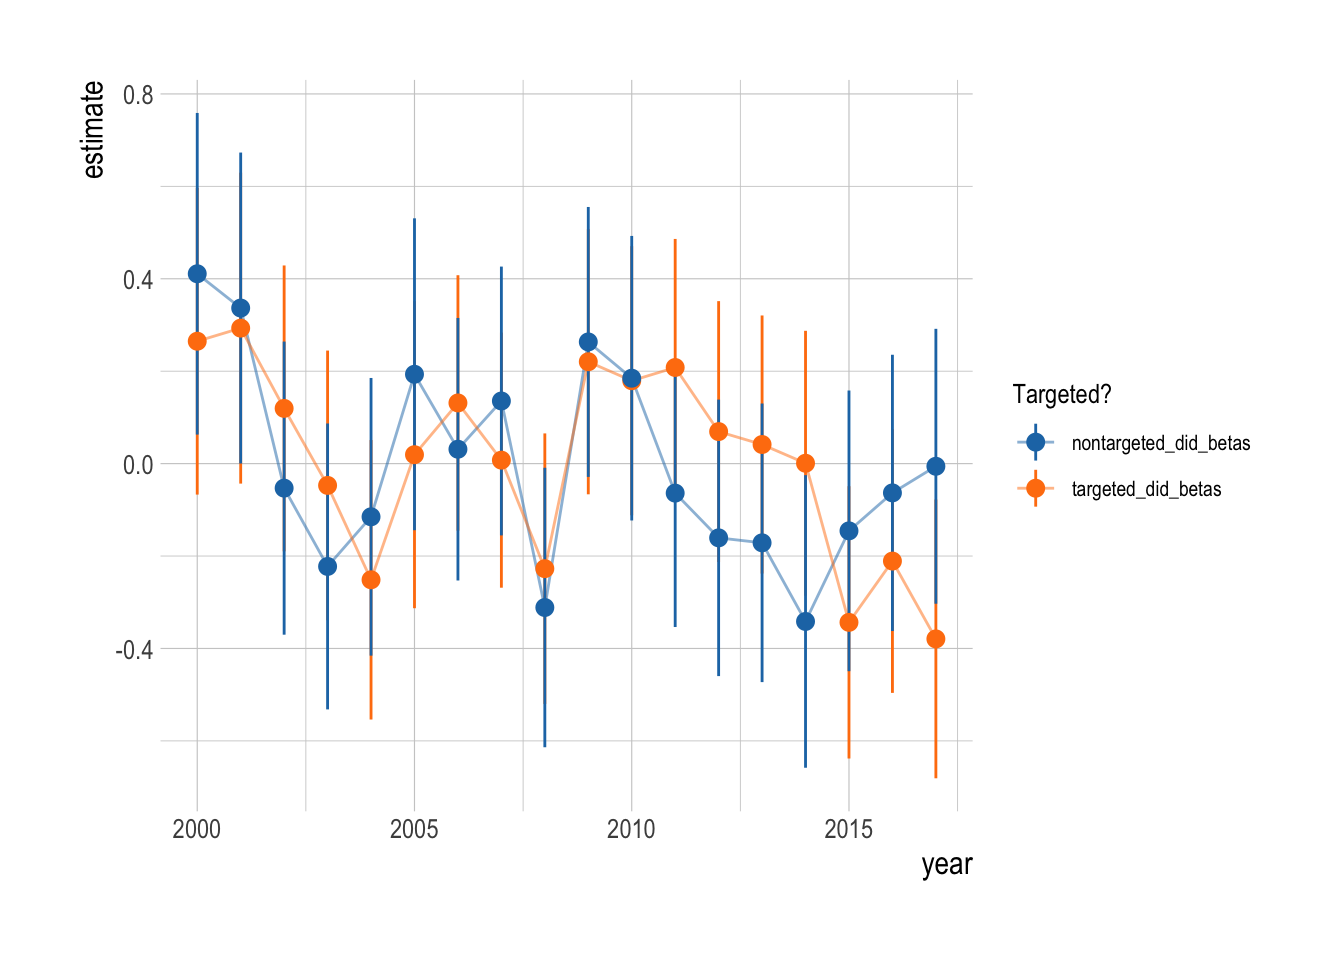
\includegraphics{thesis_files/figure-latex/targ-plot-1.pdf}
\caption{\label{fig:targ-plot}Trends in standardized mean abundance of
targeted and non-targeted species}
\end{figure}
\section{Supplementary Materials}\label{supplementary-materials}

\subsection{Regression Diagnostics}\label{regression-diagnostics}
\begin{figure}
\centering
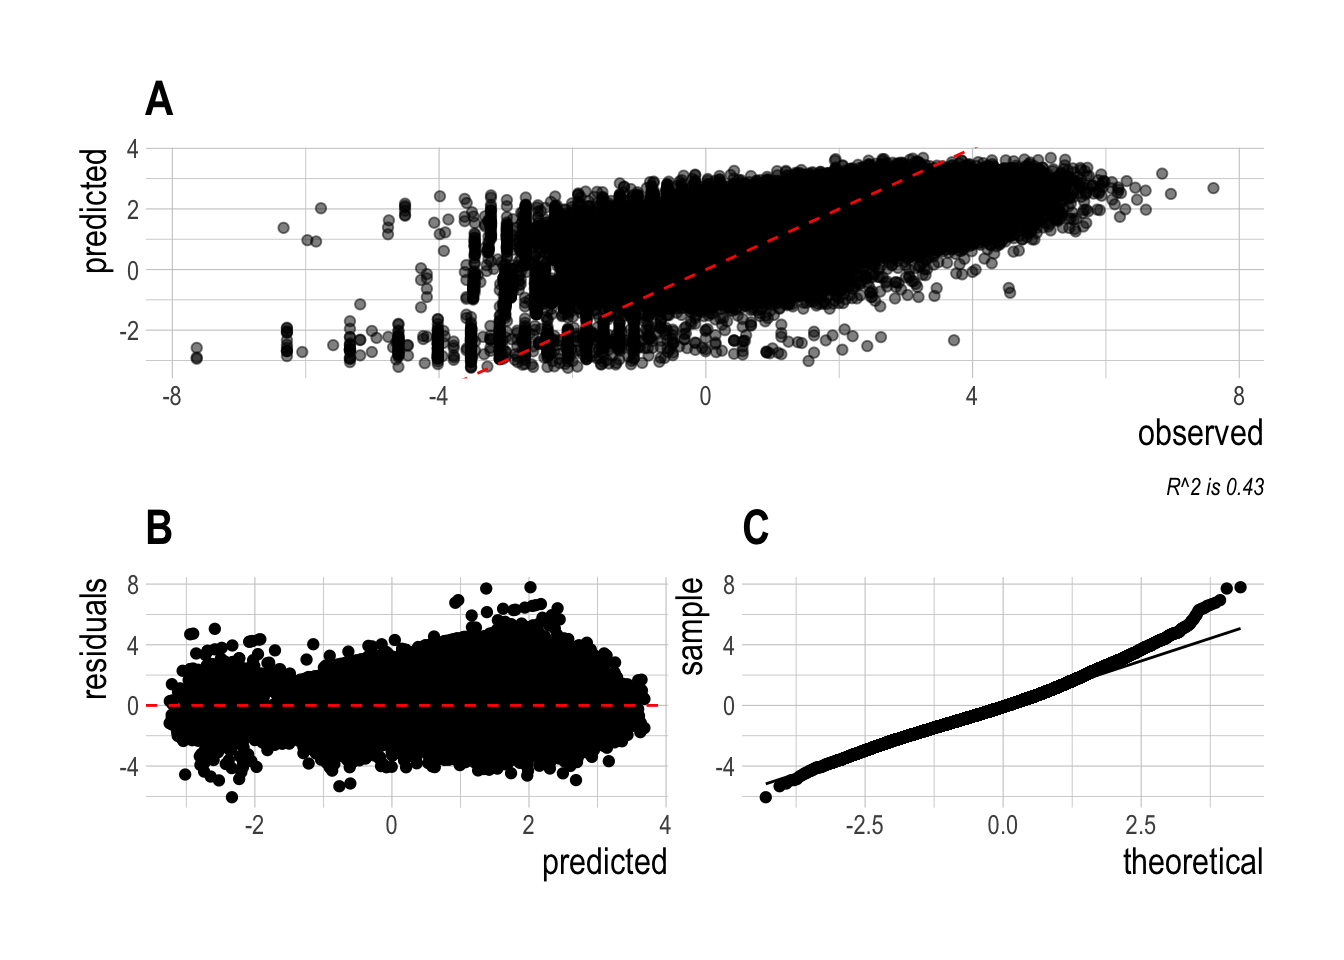
\includegraphics{thesis_files/figure-latex/obs-v-pred-1.pdf}
\caption{\label{fig:obs-v-pred}High level diagnostics for observed
compontent of Delta-GLM: Observed vs predicted log densities (A),
predicted log density vs residuals (B), and a normal qq-plot of the
residuals (C)}
\end{figure}
\begin{figure}
\centering
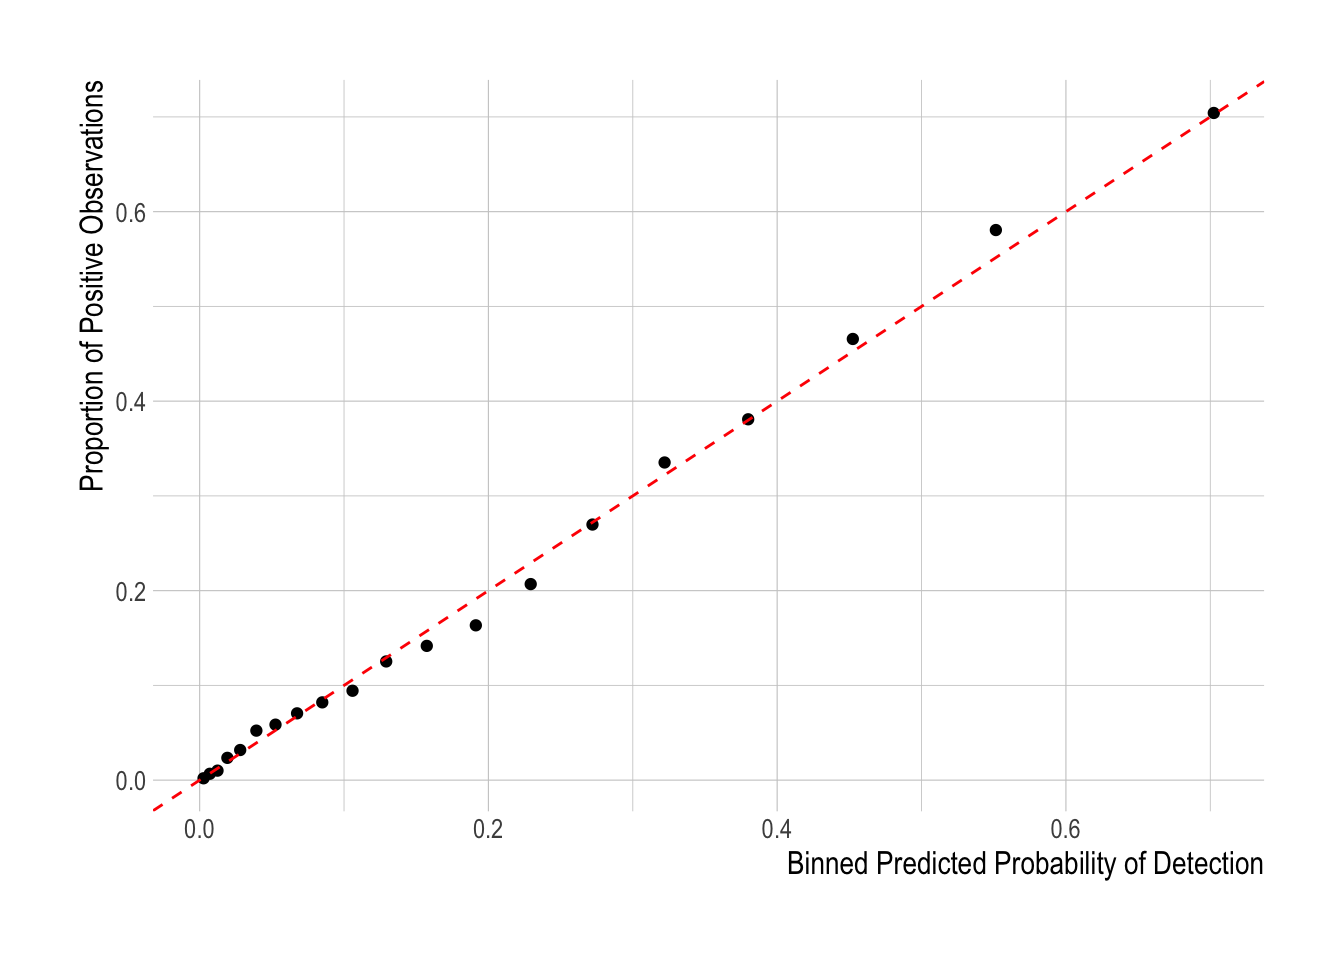
\includegraphics{thesis_files/figure-latex/unnamed-chunk-15-1.pdf}
\caption{\label{fig:unnamed-chunk-15}Binned mean predicted probability of
detection provided by the first stage of the hurdel model vs observed
proportion of positive detections}
\end{figure}
\begin{figure}
\centering
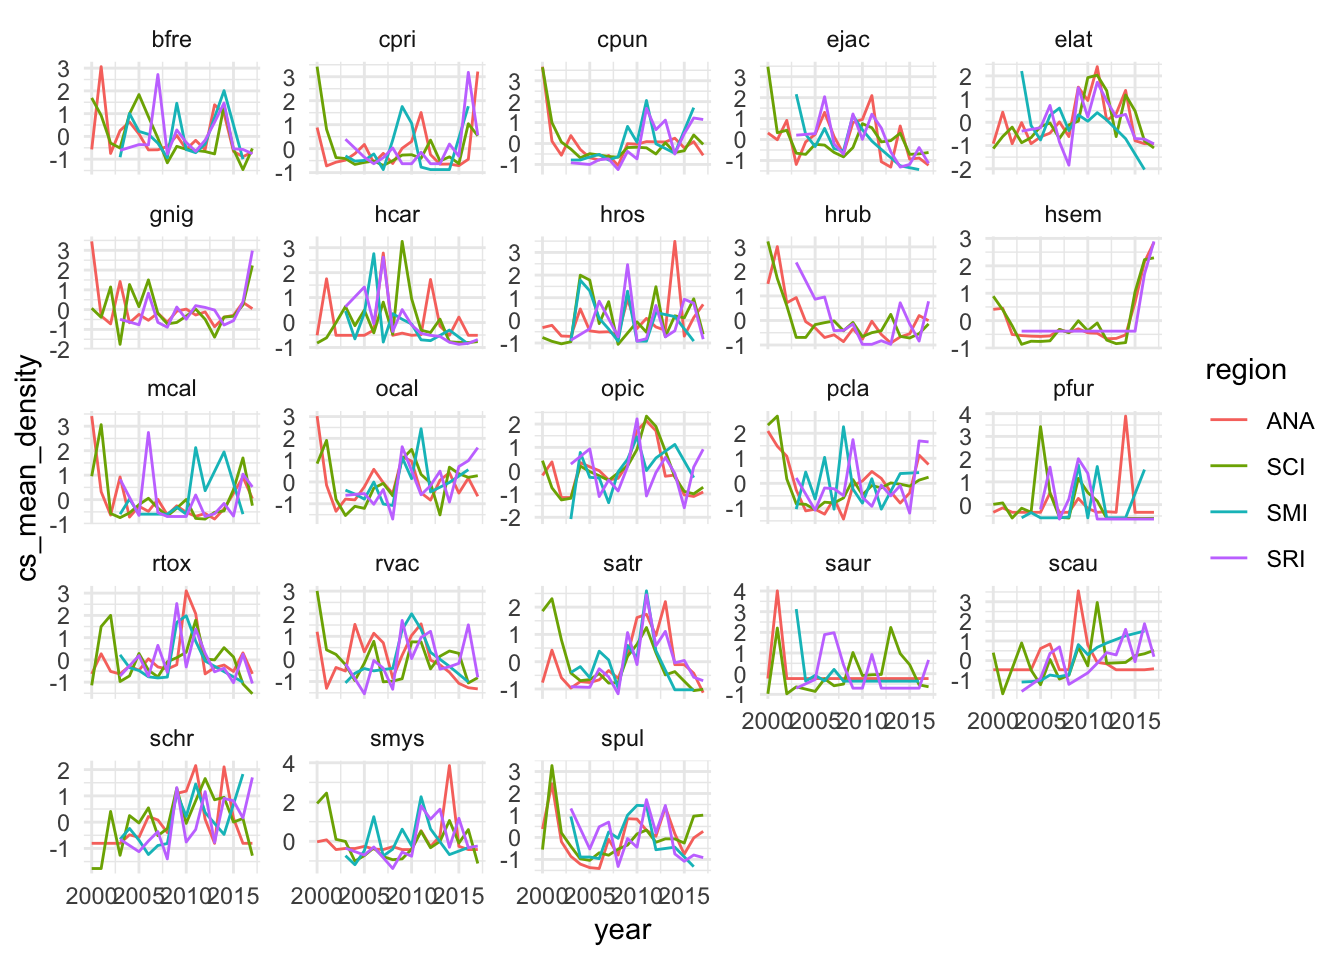
\includegraphics{thesis_files/figure-latex/reg-pop-1.pdf}
\caption{\label{fig:reg-pop}Mean density by island by year for each fish
species included in the analysis}
\end{figure}
\begin{figure}
\centering
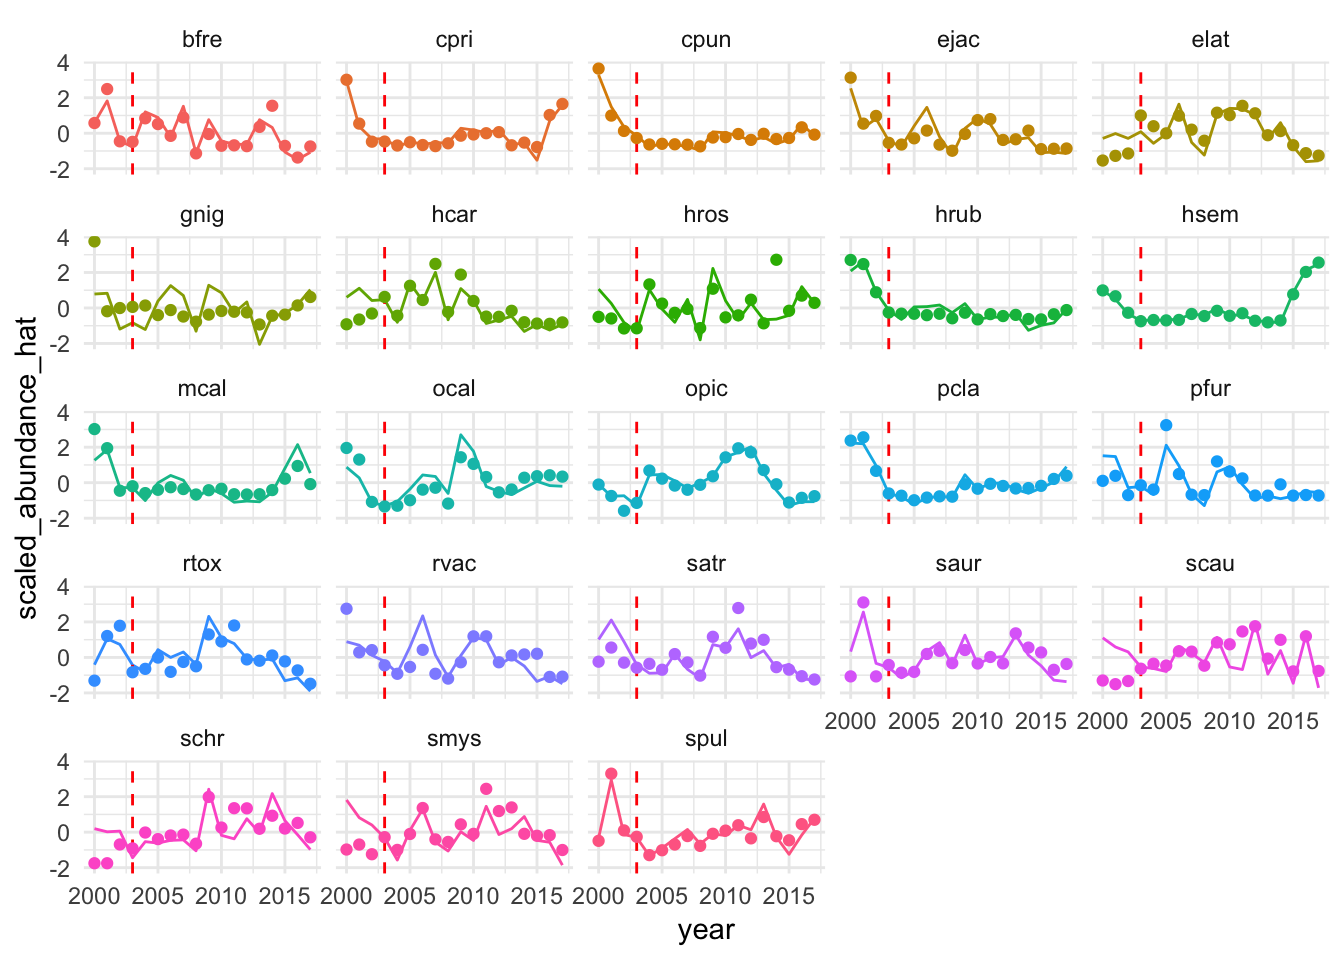
\includegraphics{thesis_files/figure-latex/raw-v-stand-plot-1.pdf}
\caption{\label{fig:raw-v-stand-plot}Raw (points) and standardized (lines)
indices of abundance for each of the fishes included in the analysis}
\end{figure}
Dealing with ``missing'' observations is a critical challenge in any
field observation study. If no observations of a given fish species were
recorded on a given transect, should the density of that species on that
transect be marked as zero, and influence the estimate of the overall
mean density accordingly? The obvious answer seems to be yes, but what
if that species simply does not live in the environment covered by a
particular transect? For our base runs, we assign a value of zero
density on a given transect for any fish species that has been observed
at least once at a given site at any time in our data but was not
observed on that particular transect. If that species was never observed
at that site, we do not include a zero for that species. Our rationale
for this is that given the shifting nature of the sampled sites, and the
intensity of sampling at those sites, we do not want to skew density
trends by changes in the amount of suitable habitat for a given species
sampled. However, this is clearly a strong assumption. For example,
perhaps the decreasing trend in mean densities from 2000 to 2004 is due
to increased number of sites (and therefore zeros) included in the data.
To assess the potential importance of this choice, we can compare the
mean densities of targeted and non-targeted species over time with the
added zeros (Fig.\ref{fig:raw-trend}) to the mean densities using only
positive observations (i.e.~not including any zeros in the data,
(Fig.\ref{fig:nozero-raw-trend}). The trends in the raw densities, and
most importantly the mean trends of targeted and non-targeted fishes,
are nearly identical whether or not zeros are added, providing strong
evidence that our choice of how to incorporate missing observations into
the data are not strongly influencing our overall results.
\begin{figure}
\centering
\includegraphics{thesis_files/figure-latex/nozero-raw-trend-1.pdf}
\caption{\label{fig:nozero-raw-trend}Centered and scaled mean annual
density, excluding zeros, of included fishes (points) and smoothed means
of targeted and non-targeted groups (line) over time}
\end{figure}
We include a variety of environmental, observation, and temporal
indicators in our model. Inclusion of highly co-linear variables in a
model can inflate standard errors and obscure ``true'' effects. To
account for this we calculated the Pearson's correlation coefficients
for all of the continuous data included in our model to ensure that none
of the included variables had correlation coefficients greater than 0.7,
a general rule of thumb for co-inclusion of variables. We did not find
problematic levels of correlation among any of our included continuous
variables.
\begin{figure}
\centering
\includegraphics{thesis_files/figure-latex/numeric-cor-1.pdf}
\caption{\label{fig:numeric-cor}Pearson correlation coefficients of
continuos data included in the regression model}
\end{figure}
\subsection{Selection on Observables}\label{selection-on-observables}

Our proposed identification strategy attempts to control for non-MPA
(and not directly modeled) related changes in abundances through the
trend in the non-targeted species. However, a simpler alternative would
be to simply compare densities before-and-after MPA implementation,
while explicitly controlling for non-MPA related factors that we believe
may have some effect on densities (a ``selection on observables''
strategy). To that end, we fit a mixed-effects regression that models
log densities (of positive observations only for simplicity's sake here)
as a function of temperature deviations, kelp cover, observer
experience, random effects for species and region, and fixed effects for
each year in the data (omitting the year 2000).

Using this model, densities of targeted species appear to have been
declining steadily since 2000, and appear to have plateaued off since
the implementation of MPAs in 2003. Without an identification strategy
such as the one employed in this study then, all we could conclude is
that densities appear to be lower post-MPA, and have not increased
substantially over time (Fig.\ref{fig:obs-plot}).
\begin{figure}
\centering
\includegraphics{thesis_files/figure-latex/obs-plot-1.pdf}
\caption{\label{fig:obs-plot}Selection on observables identification
strategy. Plotted estiamtes are fixed effects of year on log-density
(relative to the year 2000), controlling for observer experience,
temperature deviations, and kelp cover, with random effects for species
and region}
\end{figure}
\subsection{Repeat basic analysis.}\label{repeat-basic-analysis.}

This analysis has a LOT of complicated moving parts. It's worth taking a
step back and keeping it simple though: what does a simple classic
difference in difference analysis say? i.e.
\texttt{targeted\ +\ year\ +\ year:targeted}, aggregating up the
densities to take care of the zeros. The results of this basic analysis
do tell a different story than our complex über model, indicating broad
evidence for a positive regional MPA effect, as measured by the
divergence between the targeted and non-targeted. However, we have
several reasons to be skeptical of this simplified assessment. First,
the error bars are massive here, with effect sizes reaching up to 400\%,
which our simulation analysis suggests should be unlikely. Second,
taking this simplified assessment at face value would suggest that the
divergence between the targeted and non-targeted was at near its highest
level in 2013, the first year the MPA went in place, suggesting a
massive and immediate effect, if we were to take this regression at face
value. For these reasons, we do not feel that the simplified regression
represents a more accurate result than our mode complete and complex
model. Rather, if we simply examine the trend in the simple analysis,
rather then the levels, the trend matches our other results (flat, up,
and then down). We hypothesize then that our full model acts to 1)
vastly reduce the span of the error bars around our estimated divergence
between targeted and non-targeted fishes, and 2) remove bias in the
effect introduced by covariates (Fig.\ref{fig:basic-plot}.
\begin{figure}
\centering
\includegraphics{thesis_files/figure-latex/basic-plot-1.pdf}
\caption{\label{fig:basic-plot}Simple DiD using aggregate Density Data}
\end{figure}
\chapter{Improving Fisheries Stock Assessment by Integrating Economic
Theory and Data}\label{scrooge}

\section{Abstract}\label{abstract}

The well-being of coastal communities and ecosystems around the world
depends on our ability to provide accurate and timely assessments of the
status of fished populations. This is typically accomplished by
collecting biologically-focused data such as the amount and size of fish
captured, and using those data to fit statistical models that estimate
factors such as current biomass levels and exploitation rates, usually
relative to some benchmark set by stakeholders.

This stock assessment process has had successes throughout the world
especially where the data and resources are available to perform what we
might call ``traditional'' statistical stock assessments (Hilborn and
Ovando \protect\hyperlink{ref-Hilborn2014b}{2014}). While many of the
world's largest and most valuable fisheries fall into this category, the
majority of people that depend on fisheries do so in smaller scale
operations that lack the capacity for traditional stock assessment, a
group that has been generally called ``data limited fisheries''. This
problem has led to an explosion of ``data limited stock assessments''
(DLAs), that aim to provide management advice using fewer data (but more
assumptions). These DLAs have made fisheries assessment possible in
previously unassessed places, but increasingly they have sought to
simply use more involved statistics to extract more knowledge from the
same data (often length composition of the catch).

This study improves the management capacity of data-limited fisheries by
demonstrating how expanding the pool of available data to include
economic and biological information together can improve the accuracy of
stock assessments. While fisheries are coupled socio-ecological systems
(Ostrom \protect\hyperlink{ref-Ostrom2009}{2009}), the human dimensions
of fisheries, the incentives that drive behavior, have been left to
economists and other social scientists, while the stock assessment side
of the equation has focused on the ecological and biological aspects of
a fishery. Our results build off of fisheries economics to show that
utilizing data on the economic history of a fishery (prices, costs,
technology, labor, and profitability) together with biological data can
improve the ability of stock assessment models to accurately estimate
fishing mortality rates. In many realistic simulations, we demonstrate
that this bio-economic estimation model provides more accurate results
than published methods utilizing biological data alone. Lastly, we
provide a generalizable simulation framework using machine learning
techniques to assess the the relative performance of these models under
different states of nature.

Our results demonstrate how often available, but to date underutilized,
data can improve stock assessment in data-limited contexts. While we
present one specific methodology for incorporating economic data into
stock assessment, these results can serve as a foundation for a broader
field of study investigating methods for utilizing economic data in
biological stock assessment, improving both the accuracy and
effectiveness of fisheries management around the globe.

\section{Introduction}\label{introduction-3}

Effective fisheries management requires that managers and stakeholders
have some ability to estimate and react to the abundance of fishes in
the ocean in a timely manner. The history of fisheries science has been
largely concerned with developing and improving our ability to
accomplish this difficult task, starting from early models of growth
overfishing (as described in Smith
\protect\hyperlink{ref-Smith1994}{1994}) and leading up to multi-species
bio-economic models (e.g. Plagányi \emph{et al.}
\protect\hyperlink{ref-Plaganyi2014}{2014}). While the field has made
dramatic advances in our ability to assess the status of fisheries, by
and large we have found two solutions to the problems of stock
assessment: Fit highly complex integrated statistical models to diverse
data streams, or utilize increasing levels of statistical wizardry to
try and squeeze more information out of limited data (what has lately
been termed Data Limited Stock Assessments, or DLAs). The explosion of
DLAs has been both promising and concerning. The majority of fisheries
in the world lack the resources for fully integrated stock assessments,
and so depend on this world of ``data limited stock assessment''. While
there has been tremendous growth in this field, nearly all DLAs rely on
the same streams of information that would have been available to a
fisheries scientist in the 1800s: lengths, captures, and catch per unit
effort, generally only one at a time. While these biological data can be
highly informative, economic data can also provide information as to the
history and status of a fishery. We present here a novel tool for
combining historic economic information with traditional fisheries data
to improve fisheries stock assessment.

Why do we need a new line of evidence in stock assessment? One could
certainly make the case that statistical stock assessments are
complicated enough as it is. But, while these ``gold standard''
assessments (usually) perform well using solely biological data,
data-limited stock assessments, in which models are fit by trading in
data for assumptions, often struggle if the exact requirements of their
assumptions are not satisfied. This can present a major problem for
communities and ecosystems that depend on the outcomes of these DLAs to
guide their management practices. While future work can examine the
usefulness of economic data in a data-rich context, our focus here is in
demonstrating how economic information augment biological data to
improve the performance of data-limited stock assessments.

What defines a data limited assessment? Dowling \emph{et al.}
(\protect\hyperlink{ref-Dowling2015}{2015}) provides a useful summary of
what we mean by a data-limited fishery, but for now we can broadly
consider data-limited assessments as fisheries lacking sufficient
quality information to perform a ``traditional'' stock assessment,
meaning at minimum total catch records and catch-per-unit-effort, on up
to a fully integrated statistical catch-at-age model requiring catch,
CPUE, length compositions, growth and aging, tagging, etc. A common
example of a data-limited fishery would be a fishery for which only CPUE
data is available, or for which the only species-specific information
are sampled length frequencies from the port or market.

This paper builds off the length-based DLA literature, and so we focus
our discussion on the nature of these methods. See Carruthers \emph{et
al.} (\protect\hyperlink{ref-Carruthers2014}{2014}) and Anderson
\emph{et al.} (\protect\hyperlink{ref-Anderson2017b}{2017}) for thorough
summaries of catch-based DLAs. Length-based DLAs all use life history
data or assumptions of some kind to translate the distribution of
observed lengths in a fished population into some meaningful management
metric. Catch-curves, perhaps the oldest of the DLAs, dating back to at
least Chapman and Robson (\protect\hyperlink{ref-Chapman1960}{1960}),
use assumptions and estimates of the age-at-length relationship to
translate lengths into ages, and measure the slope of the logarithm of
the numbers at age to provide an estimate of total mortality \emph{Z}.
Assumptions or estimates of natural mortality \emph{m} can then be used
to extract fishing mortality \emph{f} simply by \(f = Z - m\). Recently,
newer methods have evolved that try and estimate fishing mortality
rates, recruitment, and selectivity by examining the overall shape of
the length composition data (Hordyk \emph{et al.}
\protect\hyperlink{ref-Hordyk2014}{2014}; Rudd and Thorson
\protect\hyperlink{ref-Rudd2017}{2017}). These models use life history
data (or assumptions) to simulate what the length composition of a given
population would be expected to be if it were left unfished. This
estimate of the unfished length composition is then compared to the
observed length composition, and estimates of fishing mortality,
recruitment, and selectivity are made that best explain the observed
length composition, given the expectation provided by life history data.

\subsection{What's the Problem that Economic Data Could
Fix?}\label{whats-the-problem-that-economic-data-could-fix}

These existing DLA methods have proven effective and useful in many
circumstances, but their reliance on length composition leaves them
sensitive to relatively common features in fisheries such as
autocorrelated shifts in recruitment regimes. Given length data alone,
it is difficult to separate the signal of recruitment from fishing
mortality if recruitment is not relatively stable, since both manifest
themselves as change in the relative proportions of the observed length
classes. The most straightforward solution to this problem is to assume
that the population is at equilibrium, and any deviations in expected
recruitment are on average zero during the time period of analysis.
Year-to-year shifts in the length composition are then attributed to
fishing mortality. Given limited data, say only one year of length
composition data, this may be the only assumption possible.

Since recruitment regimes are likely to be more the rule than the
exception though (Szuwalski and Hollowed
\protect\hyperlink{ref-Szuwalski2016}{2016}; Munch \emph{et al.}
\protect\hyperlink{ref-Munch2018}{2018}), we would like to be able to
relax this key assumption of stable recruitment. Rudd and Thorson
(\protect\hyperlink{ref-Rudd2017}{2017}) provided an important extension
to the equilibrium assumptions underpinning Hordyk \emph{et al.}
(\protect\hyperlink{ref-Hordyk2014}{2014}) by relaxing the equilibrium
assumption and allowing the user to estimate a vector of recruitment
deviates and fishing mortality rates given a time series of length
composition data. In order to get around the confounded nature of
recruitment and fishing mortality, given only length data the LIME model
presented in Rudd and Thorson (\protect\hyperlink{ref-Rudd2017}{2017})
requires a user specified penalty constraining the amount that fishing
mortality can vary year-to-year. More importantly though, LIME provides
a flexible tool for integrating multiple forms of data that while still
potentially less than what would go into a ``traditional'' assessment
are together still informative. LIME is an important tool for
integrating multiple streams of ``limited data'' together into a
comprehensive assessment. However, the data types that can be
incorporated into LIME are all components of the traditional fisheries
toolbox: lengths, catches, and CPUEs. While these data are important and
useful, we present a new model, \texttt{scrooge}, that builds on the
foundation provided by LIME to expand the set of possible assessment
inputs to include economic theory and data.

Why should we expect economic theory and data to be useful? Fisheries
are dynamic bio-economic systems, in which the behavior of fishing
fleets affect fish populations, and changes in fished populations affect
fishing behavior. This idea was first formalized by Gordon
(\protect\hyperlink{ref-Gordon1954}{1954}), which sought to explain the
evolution of fishing fleets through an open-access model of rent
seeking, which results in a fishery reaching an open-access equilibrium
where total profits are zero. While this simple model has been vastly
expanded on since then, the core idea remains that we can construct
models linking human incentives and ecological dynamics to explain
fishing behavior.

Bio-economic modeling has most commonly been utilized in the management
strategy evaluation (MSE) (summarized in Punt \emph{et al.}
\protect\hyperlink{ref-Punt2016a}{2016}) phase of fisheries management.
Early design on management policy centered on identifying the best
strategy to employ (e.g.~the right size limit or quota), under the
assumption that once implemented the policy would be gospel. However,
the real world is not often so kind: fishermen respond to incentives and
regulations, and therefore what happens on the water is often not what
managers had in mind when a regulation was put in place (Salas and
Gaertner \protect\hyperlink{ref-Salas2004}{2004}; Branch \emph{et al.}
\protect\hyperlink{ref-Branch2006}{2006}; Fulton \emph{et al.}
\protect\hyperlink{ref-Fulton2011}{2011}). As a result of this reality,
a growing body of work has sought to build the behavior of fishing
fleets into the MSE process, in order to estimate how a policy might
actually play out once real people come into contact with it. Nielsen
\emph{et al.} (\protect\hyperlink{ref-Nielsen2017}{2017}) and van Putten
\emph{et al.} (\protect\hyperlink{ref-vanPutten2012}{2012}) provide a
useful summaries of the large number of models that utilize some form of
integrated economic-ecological modeling in the evaluation of management
strategies.

Each of these models vary in the structure and complexity with which
they model economic behavior, but they share a common feature that they
are all focused on the forecasting phase of management, leaving the task
of understanding the status of the fishery today to stock assessment
models. Thorson \emph{et al.}
(\protect\hyperlink{ref-Thorson2013a}{2013}) provides one of the only
examples of which we are aware of that explicitly incorporates effort
dynamics informed by bio-economic theory into the stock assessment
process through a state-space catch only model (SSCOM) (though Hilborn
and Kennedy \protect\hyperlink{ref-Hilborn1992a}{1992} demonstrates the
linkages between effort distributions and spatial population structure).
Thorson \emph{et al.} (\protect\hyperlink{ref-Thorson2013a}{2013})
demonstrates that incorporation of effort dynamics can improve the
estimation of biomass from catch data. The model functions by estimating
open-access style parameters that serve as aggregate indices of economic
conditions in a fishery. However, these economic parameters are not
directly informed by economic data; rather priors for these parameters
are develop by fitting to observed dynamics of biomass and effort, and
these priors are then updated through confrontation with catch data in
SSCOM.

In summary, a large body of literature exists showing there exist
predictable dynamics between fishing effort and fished populations. Our
proposed method builds off this literature in a similar manner to LIME
and SSCOM, by hypothesizing that priors informed by economic theory can
improve the ability of an assessment model to make sense of limited
data. However, we extend this concept to utilize economic data to inform
the economic parameters in our model. Specifically, we demonstrate how
data on changes in prices, costs, technology, profits, and effort can be
utilized to estimate bio-economic parameters that improve the ability of
a primarily length-based assessment method to estimate fishing mortality
rates.

\section{Methods}\label{methods-3}

Overview:
\begin{itemize}
\item
  We utilize an age-structured bio-economic operating model to create a
  database of simulated fisheries
\item
  Fishing mortality rates from the simulated fishery are estimated using
  \texttt{scrooge}, our bio-economic estimation model
\item
  We assess the performance of different configurations of
  \texttt{scrooge} using a set of case study fisheries
\item
  We assess broader model performance using a Bayesian hierarchical
  model and classification algorithms
\end{itemize}
\subsection{Why A Bayesian Approach?}\label{why-a-bayesian-approach}

Bayesian methods play an important role in fisheries science.
Informative priors can help parameterize challenging functions such as
the stock-recruitment relationship, and the outcomes of Bayesian
assessment provide estimates of posterior probability of states of
nature, greatly aiding the management strategy evaluation process (Punt
and Hilborn \protect\hyperlink{ref-Punt1997}{1997}; Myers \emph{et al.}
\protect\hyperlink{ref-Myers2002}{2002}). While decisions about prior
distributions can in some cases dramatically affect assessment accuracy
(Thorson and Cope \protect\hyperlink{ref-Thorson2017a}{2017}), properly
implemented Bayesian methods can provide improved estimates of
uncertainty over maximum likelihood approaches (Magnusson \emph{et al.}
\protect\hyperlink{ref-Magnusson2013}{2013}).

While there are statistical reasons to favor (and in some circumstances
resist) a Bayesian approach to fisheries assessment, our choice of a
Bayesian method here is to provide a quantitative framework for bringing
local knowledge into the fisheries stock assessment process. To our
knowledge, the use of informative priors in data-limited fisheries has
focused on biological traits such as growth rates (Jiao \emph{et al.}
\protect\hyperlink{ref-Jiao2011}{2011}) or depletion (Cope
\protect\hyperlink{ref-Cope2013}{2013}), and in general Bayesian
processes that make strong use of informative priors (i.e.~aren't just
using Bayes for the MCMC) are rare in the data-limited assessment world.
We find this general fact somewhat surprising: Bayesian methods can be
particularly useful in ecological model fitting when ``hard'' local data
are limited but prior knowledge is available (Choy \emph{et al.}
\protect\hyperlink{ref-Choy2009}{2009}), as is often the case in
data-limited fisheries. In other words, a fishery can be data-limited
but knowledge-rich, and a Bayesian process provides a clear statistical
framework for incorporating this prior knowledge into the model-fitting
process. In addition, it is very common in data-limited contexts to have
noisy data that do not paint a clear picture, even after careful
statistical analysis. A Bayesian framework allows us to express these
uncertain results as posterior probabilities, making statements such as
``our model says there is a 75\% chance that we are overfishing the
population'' possible, which are not as feasible in a frequentist
setting without approximation methods such as bootstrapping or the delta
method. The core hypothesis behind our model is that economic data can
inform stock status. While economic data in the form of official
government statistics maybe hard to come by, we believe that in these
cases economic histories can be elicited from stakeholders. We selected
a Bayesian methodology then as an explicit way of bringing this economic
knowledge, whether qualitative or quantitative, into the fisheries stock
assessment process.

\subsection{Simulation Model}\label{simulation-model-1}

We simulate different fisheries defined by their biological (e.g.~fast
vs.~slow growing, stochastic vs.~deterministic recruitment) and economic
(e.g.~open-access vs.~constant effort) characteristics. Length
composition and economic data are then collected from the simulated
fishery, and used in our assessment method. Outcomes of the assessment,
in this case estimated fishing mortality rates, can then be compared to
the true fishing mortality rate experienced by the fishery in that
simulation. The simulation model itself is a age-structured
single-species bio-economic model, in the form described by Ovando
\emph{et al.} (\protect\hyperlink{ref-Ovando2016a}{2016}). A given
simulation starts by selecting a species. Core life history data for
that species (growth, mortality, maturity) are then drawn from the
\texttt{FishLife} package in R (Thorson \emph{et al.}
\protect\hyperlink{ref-Thorson2017d}{2017}). However, the user can set a
number of important specific biological traits for that fishery. For
example, the user can specify both the coefficient of variation and
autocorrelation of recruitment deviates, and the timing of density
dependence (e.g.~pre-or-post settlement). On the economic side, for a
given simulation the user specifies an initial level of fishing
mortality at the start of the fishery, from which dynamics evolve. The
effort dynamics are governed by a wide set of specifiable parameters,
such as prices, costs, and catchability, all of which can be supplied a
coefficient of variation, autocorrelation, and drift. Users also specify
the length at 50\% selectivity, and the relative profitability of the
fishery. The user specifies a fleet model, which can be one of
open-access (effort changes in proportion to profit per unit effort in
the previous time step), constant-effort (effort stays at the specified
initial effort, though fishing mortality rates resulting from this
effort can shift if catchability changes over time), or random-walk
(effort follows a random walk process from year to year). Across all of
these fleet models, users can also specify a coefficient of variation
and autocorrelation for deviations from these effort dynamics.

While this operating model is still a large simplification of a real
fishery, we incorporate critical traints for evaluating the performance
of our assessment model. First, we allow for both recruitment and
fishing mortality to shift over time, which will dramatically affect the
ability of length-based assessments to perform. Second, we allow for
economic data to change over time (e.g.~increasing prices), and for
these changes to affect the evolution of the fishery through the
open-access dynamics model. Third, we can simulate scenarios during
which economic data change, but these changes do not translate into
changes in effort. In sum then, this operating model allows us to test
scenarios that satisfy the assumptions of a biological length-based DLA,
that violate those assumptions but satisfy economic assumptions, and
that violate both. This provides an diverse sandbox of simulations to
test the performance of our proposed assessment method.

\subsection{\texorpdfstring{\texttt{scrooge}
Model}{scrooge Model}}\label{scrooge-model}

Since our model assumes that fishing behavior is driven by profits, we
for call our proposed model \texttt{scrooge} (this probably won't last
in publication, but I like it for now). \texttt{scrooge} can be run
using a variety of different combinations of effort process models
(e.g.~random walk vs open-access) and likelihood structures (e.g.~length
composition). We use the form
\texttt{economic\ process\ model/likelihood\ components} to denote a
configuration. For example a configuration of \texttt{random-walk/lcomp}
means the model uses a random walk effort process model and includes
only length composition data in the likelihood. We assess factorial
combinations of process models and likelihoods, omitting combinations
that would double count data (e.g.~using profit per unit effort data
both in the likelihood). See Table.\ref{tab:model-table} for a summary
of all of the configuration components.
\begin{table}

\caption{\label{tab:model-table}Candidate economic process models and likelihood components of scrooge}
\centering
\fontsize{9}{11}\selectfont
\begin{tabu} to \linewidth {>{\raggedright}X>{\raggedright}X>{\raggedright}X}
\toprule
\textbf{Name} & \textbf{Abbreviation} & \textbf{Description}\\
\midrule
\addlinespace[0.3em]
\multicolumn{3}{l}{\textbf{Economic Process Models}}\\
\hspace{1em}Random Walk & random-walk & Effort evolves as a random walk independent of economics\\
\hspace{1em}Bio-economic model with profit ingredients & ingredients & Effort responds to profit per unit effort built from data on price, cost, q\\
\hspace{1em}Bio-economic model with PPUE & ppue & Effort responds to profit per unit effort, PPUE data supplied\\
\hspace{1em}Effort Data & effort & Effort is adjusted by data on proportional changes in effort\\
\addlinespace[0.3em]
\multicolumn{3}{l}{\textbf{Likelihood Components}}\\
\hspace{1em}Lengths & lcomp & Length composition data are the only part of the likelihood\\
\hspace{1em}Lengths + PPUE & lcomp+ppue & Likelihood composed of PPUE and length composition data\\
\hspace{1em}Lengths + Porportional Effort & lcomp+effort & Likelihood composed of percent changes in effort and length composition data\\
\bottomrule
\end{tabu}
\end{table}
\begin{table}

\caption{\label{tab:prior-table}Model parameters and prior distributions}
\centering
\fontsize{9}{11}\selectfont
\begin{tabu} to \linewidth {>{\raggedright}X>{\raggedright}X>{\raggedright}X}
\toprule
\textbf{Parameter} & \textbf{Transformations} & \textbf{Prior}\\
\midrule
Initial Fishing Mortality & N/A & $f^{init} \sim halfnormal(0,1)$\\
Log Rec. Dev & $RecDev = exp(\sigma_{r}LogRecDev - \sigma_{r}^2/2)$ & $LogRecDev \sim normal(0,1)$\\
Log Effort Dev & $EffDev = exp(\sigma_{e}LogEffDev - \sigma_{e}^2/2)$ & $LogEffDev \sim normal(0,1)$\\
$\sigma_r$ & N/A & $\sigma_r \sim halfnormal(0.4,0.4)$\\
$\sigma_{obs}$ & N/A & $\sigma_{obs} \sim halfnormal(0,2*sd(DATA))$\\
\addlinespace
$\sigma_e$ & N/A & $\sigma_e \sim halfnormal(0.2,0.2)$\\
Max Percent Change Effort & N/A & $MaxPercEffort \sim halfnormal(0, 0.25)$\\
Cost to Revenue Ratio & N/A & $crRatio \sim halfnormal(0.5, 1)$\\
50perc sel as percent of linf & N/A & $p50Sel \sim halfnormal(UserGuess, 0.05)$\\
\bottomrule
\end{tabu}
\end{table}
The estimating model itself was coded in Stan (Carpenter \emph{et al.}
\protect\hyperlink{ref-Carpenter2017}{2017}) using the \texttt{rstan}
package (Stan Development Team
\protect\hyperlink{ref-StanDevelopmentTeam2018}{2018}). The core
internal operating model is an age structured model identical in
structure to the operating model used for the simulations. This means
that the model requires user-supplied estimates of life history data,
specifically
\begin{itemize}
\item
  Von Bertalanffy growth parameters
\item
  Allometric weight and maturity at length/age equations
\item
  An estimate of natural mortality
\item
  An estimate of Beverton-Holt steepness
\end{itemize}
We constructed four candidate effort process models describing the
effort dynamics of the fishing fleet, and three candidate likelihood
structures, each defined by different structural assumptions and data
availability. We then fit factorial combinations of each effort process
model with each likelihood structure, omitting combinations that would
have double counted some information as both a prior and data.

The model has a number of parameters it must estimate, namely fishing
mortality rates, recruitment deviates, the length at 50\% selectivity,
and associated process and observation errors as required (see
Table.\ref{tab:prior-table} for a complete description of all estimated
parameters and their prior distributions). The model is initialized at
unfished biomass, and then an estimate of initial fishing mortality is
applied for 100 burn-in years, achieving a level of depletion at the
start of the data-period of the model. The data period of the model is
of length \emph{t}, and defines the time-steps during which the model
estimates dynamic parameters, though the model estimate \emph{t} + age
50\% selectivity recruitment deviates, to allow the model to estimate
recruitment pulses which start before the data-period but whose signal
can be observed during the early years of the data period.
Length-composition data must be available for 1 or more years of the
data-period, but are not required in all years. For example, the model
can function if given ten years of economic information and only one
year of length composition data available at the end of the time period.

All estimation models share common components of recruitment deviates
and length composition data. Recruitment is assumed to on average have
Beverton-Holt dynamics (Beverton and Holt
\protect\hyperlink{ref-Beverton1959}{1959}), reparemeterized around
steepness. Process error around this mean relationship is assumed to be
log-normally distributed with a bias correction

\[r_{t} = BH(SSB_{t-1},h)e^{r^{dev}_{t}-\sigma_{r}^2/2}\]

\[r^{dev}_{t} = \sigma_rLogRecDev_t\]

\[\sigma_r \sim halfnormal(0.4,0.4)\]

\[LogRecDev_t\sim normal(0,1)\]

Length composition data are structured as discrete numbers of fish
counted within one cm length bins per year. While each estimation model
differs in its methods for estimating fishing mortality rates, for a
given generated mortality rate, vector of estimated recruitment events
\(r\), and estimated selectivity \(s^{50}\), the model produces a vector
of probability of capture at length \(p^{capture}\) for each time step,
given the structural population equations of the model \(g()\).

\[p^{capture}_{t,l} \sim g(f, r, s^{50})\]

The observed numbers at length \(N_{t,l}\) are then assumed to be draws
from a multinomial distribution of the form

\[N_{t,1:L} \sim multinomial(p^{capture}_{t,1:L})\]

The key difference in the estimation models is how they estimate
\emph{f} and the data that enter the likelihood. All estimation of
\emph{f} begins by estimating a parameter \(f^{init}\), which is the
fishing mortality rate that is held constant over a burn-in period to
achieve a given level of depletion by the time of the start of the data
period of the model. The estimation models diverge from there in that
each specifies a different structural model for how \emph{f} evolves
from \(f^{init}\).

\subsubsection{Effort Process Models}\label{effort-process-models}

All effort process model have an expected process and a process error
component. The process error, \(E^{dev}\), is estimated in the same
manner across all the process models

Effort deviates \(E^{dev}\) are assumed to be log-normally distributed

\[E^{dev}_{t} = \sigma_ELogEDev_t\]

\[\sigma_E \sim halfnormal(0.2,0.2)\]

\[LogEDev_t\sim normal(0,1)\]

The multiplicative effort deviate is then

\[e^{E^{dev}_{t} - \sigma_e^2/2} \]

\paragraph{\texorpdfstring{Random Walk Model
(\texttt{random-walk})}{Random Walk Model (random-walk)}}\label{random-walk-model-random-walk}

This estimation model is similar in flavor to the penalty on deviations
in fishing mortality used in LIME. The initial effort is calculated as

\[E_{1} = \frac{f^{init}}{q}e^{E^{dev}_{1}-\sigma_{E}^2/2}\]

\[f_{1} = qE_{1}\]

Where \emph{q} is a catchability coefficient, held at 1e-3.

For the remaining \emph{T} time-steps, effort evolves as a random walk

\[E_{t} = E_{t-1}e^{E^{dev}_{t}}\]

\[f_{t} = qE_{t}\]

\paragraph{\texorpdfstring{Bioeconomic Model with Profit Ingredients
(\texttt{ingredients})}{Bioeconomic Model with Profit Ingredients (ingredients)}}\label{bioeconomic-model-with-profit-ingredients-ingredients}

We now turn to our class of bio-economic effort models. Across all
evaluated bio-economic models, we assume open-access dynamics where
fishermen respond to average not marginal profits, per Gordon
(\protect\hyperlink{ref-Gordon1954}{1954}), which we quantify as profits
per unit effort, or \emph{PPUE}. Under the \texttt{ingredients} model,
the user supplies some data on absolute or relative changes in prices
\emph{p}, costs \emph{c}, and technology (catchability) \emph{q}, all of
which can be thought of as ingredients of profitability. For example,
users could report a 25\% increase in prices due to the arrival of a new
buyer with access to a lucrative foreign market, a 10\% decrease in
fishing costs due to a government fuel subsidy, and/or a increase in
catchability due to the introduction of fish-finder technology. These
ingredients of profitability can be provided either as qualitative
information or hard data. Any ingredients for which no estimates of
relative rates of change are available are assumed to remain constant
over the time period of the model. The key feature of this model is that
it uses these ingredients to inform our prior estimate of profit per
unit effort, \(PPUE_{t}^*\), in a given time step. Therefore, if costs
go down and prices go up in a given time step, our estimate of
\(PPUE_{t}^*\) will increase appropriately, subsequently increasing our
prior on the amount of effort in the following time-step.

Under this model, \(PPUE_{t}^*\) is calculated as

\[PPUE_{t}^* = \frac{p_{t}C(q_{t},B_{t},E_t,s^{50}) - c_{t}E_{t}^2}{E_{t}}\]

where \emph{C()} represents that Baranov catch equation (Baranov
\protect\hyperlink{ref-Baranov1918}{1918}). The revenue part of this
profit model is relatively straightforward (price times catch), though
it does not allow for factors such as different prices for different
size of fish, regardless of weight (e.g.~some fish become less valuable
as they become larger and no longer fit on plates). The cost equation
implies that the ``cheapest'' units of effort are applied first
(e.g.~the most skilled fishermen, or the cheapest fishing grounds), and
marginal cost of fishing effort increases as more units of effort are
exerted (representing less skilled fishermen or costlier fishing
grounds). Papers such as Costello \emph{et al.}
(\protect\hyperlink{ref-Costello2016}{2016}) use a cost exponent of
1.27, but in order to keep things simple (and help the simulated
fisheries remain stable), we use a value of 2 here. This cost exponent
allows us to approximate heterogeneity in fishing costs implicitly
without actually modeling fleet components with differing skill.

Notice now that the components price (\emph{p}), catchability
(\emph{q}), and cost (\emph{c}) are allowed to vary over time. This is
because the model allows for user supplied information on the evolution
of these profit ingredients over time, either in the form of actual
values (e.g.~the price in a given year), or in relative changes (prices
are 10\% higher than they were last year). For the relative change
cases, user supplied inputs are converted to deviations from a mean
value and then multiplied by a default mean value set by the model. This
is the default for both \emph{q} and \emph{c}, since converting user
knowledge into the appropriate units is challenging. For a given value
of \(PPUE_{t}^*\), we calculate effort in the next time step per

\[E_{t + 1} = (E_{t} + \theta{PPUE_{t}^*})e^{E^{dev}_{t}}\]

where \(PPUE_{t}^*\) is the estimated profit per unit effort, and
\(\theta\) sets the responsiveness of effort to \(PPUE_{t}^*\). Note
that the model includes the same effort process error as utilized in the
random-walk process model. So, the profit ingredients and the
open-access assumptions provide our prior on the effort in a given time
step, but we estimate potential deviations from this prior expectation.
From there, the fishing mortality in a time step is calculated as

\[f_{t} = q_{t}E_{t}\]

One difficulty in this process is that the dynamics of the open access
model are driven by the relative profitability of the fishery, and as
such largely to the relative scale of revenue and costs. Therefore,
getting the relative magnitude of prices and costs to be correct is
important. Unfortunately, while prices can be relatively easily
determined, costs are much more difficult to obtain, especially in units
matching the exact effort units of the operating model. To solve this
problem, we estimate an additional parameter in this estimation model,
\(c^{max}\). The cost in any time is then calculated as

\[c_t  = c^{max}c^{rel}\]

where \(c^{rel}\) are the relative costs (scaled as deviations from a
mean) over time \emph{t} supplied by users. \(c^{max}\) itself is tuned
in a rather long process that results in much cleaner estimation that
can actually be provided with informative priors. Rather than estimating
\(c^{max}\) itself, we estimate a cost-to-revenue ratio at the start of
the fishery. We first estimate a guess of, given the simulated nature of
the fishery, something close to maximum revenues (assumed to come by
fishing a bit harder than natural mortality when the population is
completely unfished). We then calculate the profits associated with
these maximum revenues given a prior estimate of the cost to revenue
ratio CR.

\[PROFITS^{max} \sim  MAX(PRICE)CATCH^{B0}(1 - CR) \]

Given this estimate of \(PROFITS^{max}\), we can then back out the cost
coefficient \(c_{max}\) that, given the other parameters, would produce
those profits. Estimating the cost to revenue ratio instead of the
actual costs allows for informative priors to be set. A fishery that at
its heyday was incredible profitable will have a low cost to revenue
ratio, while a fishery that was scrapping by on its best day would have
a high cost to revenue ratio.

While the prior can be informed from local stakeholders, we set a zero
truncated normal prior on the cost ratio of

\[CR \sim halfnormal(0.5,1)\]

The other challenging parameter in the open access equation is
\(\theta\), the amount that effort changes for a one unit change in
\(PPUE\). Similarly to estimating the cost to revenue ratio instead of
raw costs, rather than estimate \(theta\) directly, we estimate the
maximum percentage change in effort from one time step to the next. As
part of the cost to revenue tuning process, we estimated the maximum
profits, and the effort that would produce those profits. Together that
provides us with the maximum expected PPUE. For a given max percentage
change (\(\Delta^{max}\)) in effort then, we calculate \(\theta\) as

\[\theta = (\Delta^{max}  E^{MAX}) / PPUE^{MAX}\]

While \(\theta\) has no intuitive sense for most stakeholders, the
maximum percentage year-to-year change in effort can be elicited from
stakeholders. For now, we assume a zero truncated normal prior on the
max expansion

\[\Delta^{max} \sim halfnormal(0,0.25)\]

The \texttt{ingredients} effort process model allows us to utilize
provided ingredients of profitability to drive our prior expectations of
the dynamics of fishing effort. Importantly, our translation of complex
parameters such as cost coefficients or the marginal effect of PPUE on
effort into interpretable parameters such as cost to revenue ratios and
maximum percent changes in effort greatly improves the ability of users
to elicit informative priors from stakeholders in real-world
applications of this method (Choy \emph{et al.}
\protect\hyperlink{ref-Choy2009}{2009}).

\paragraph{\texorpdfstring{Bioeconomic Model with PPUE Data
(\texttt{ppue})}{Bioeconomic Model with PPUE Data (ppue)}}\label{bioeconomic-model-with-ppue-data-ppue}

The \texttt{ingredients} model makes use of individual components of
profitability, under the theory that a) these data are informative to
the evolution of effort and b) these data may be easier to obtain than
for example actual mean profitability across the fishery. However, we
can also consider an effort process model in which \emph{PPUE} is
assumed to be known. While complete knowledge of average \emph{PPUE} in
a fishery is unlikely, especially in a data-limited context, survey
methods could be constructed to collect estimates of \emph{PPUE}, which
being a central part of a fisherman's business, is not an unreasonable
piece of information to think could be obtained, given the right
questions and sufficient trust (acknowledging that PPUE will likely have
many and more of the challenges in interpretation as CPUE data; e.g.
Walters \protect\hyperlink{ref-Walters2003}{2003}).

So, the the \texttt{ppue} model, rather than estimating \(PPUE_{t}^*\)
as a function of its ingredients, we simply take collected values of
\emph{PPUE} as data, and estimate effort per

\[E_{t + 1} = (E_{t} + \theta{PPUE_{t}})e^{E^{dev}_{t}}\]

We estimate \(\theta\) using the same methods described in the
\texttt{ingredients} method (estimating the maximum percent change in
year-to-year effort instead of \(\theta\) directly).

Since we no longer assume knowledge of technology changes over time, we
assume a static \emph{q}. This assumption could be relaxed in future
model runs to consider knowledge of both PPUE and technology, but for
now we make this assumption to make a cleaner distinction between the
\texttt{ingredients} model and the other models.

\[f_{t} = qE_{t}\]

\paragraph{\texorpdfstring{Effort Data Model
(\texttt{effort})}{Effort Data Model (effort)}}\label{effort-data-model-effort}

Both of the bio-economic process models (\texttt{ingredients} and
\texttt{ppue}) model the change in effort as a function of profit per
unit effort. Their key function, from the perspective of a model focused
on estimating biological fishery metrics, is to help inform estimates of
time-step-to-time-step changes in fishing mortality. To follow the old
adage ``keep it simple stupid'', we also build a model that assumes data
on the time-step-to-time-step proportional changes in fishing effort.
While such data are unlikely to be available for a fishery covering a
large and diverse geographic range, for more localized small-scale
fisheries such knowledge is not unreasonable. For example, fishing
cooperatives in Chile often maintain data on fishing effort.

Under the \texttt{effort} process model, we assume knowledge of the
proportional changes in effort over time \(\Delta^{effort}\), where

\[\Delta^{effort} = E_{t+1}^{true}/E_{t}^{true}\]

and

\[E_{t + 1} = (E_{t}\Delta^{effort})e^{E^{dev}_{t}}\]

and

\[f_{t} = qE_{t}\]

\subsubsection{Likelihood Models}\label{likelihood-models}

The effort process models represent alternative hypotheses as to the
true operating model driving the evolution of fishing effort, and partly
by extension fishing mortality, in a fishery. In other words, the
economic process models inform our prior on the evolution of effort.
However, a central motivation of this research is to diversify both the
data available to our assessment operating models (as we have done with
the use of economic data as components of Bayesian priors), and the data
with which we confront these models. The traditional core pantheon of
data with which we confront models in fisheries are abundance indices
(derived from either fishery dependent or independent sources) and
length/age composition data. We propose to add profit per unit effort
and proportional changes in effort to this group, at least as a starting
point in the data-limited context of this study.

\paragraph{\texorpdfstring{PPUE as an Index of Effort
(\texttt{lcomp+ppue})}{PPUE as an Index of Effort (lcomp+ppue)}}\label{ppue-as-an-index-of-effort-lcompppue}

We consider catch-per-unit-effort to be informative in fisheries (on a
good day) through the relationship

\[CPUE_{t} = \frac{q_{t}E_tB_t}{E_t} = q_tB_t\]

A constant or time-varying estimate of \emph{q} then is our link between
an observed CPUE data and an unobserved state of nature, \(B_t\) that we
wish to estimate.

We propose a similar use for profit per unit effort, but rather than
PPUE informing an index of abundance, it serves as an index in the rate
of change in effort (and by extension conditional on \emph{q}), fishing
mortality. If we assume that a standard open-access dynamics model is
true, then

\[E_{t + 1}^{true} = E_{t}^{true} + \theta{PPUE_{t}}\]

Simply rearranging this equation, we can provide a link between PPUE and
the change in effort as

\[PPUE_{t} = \frac{E_{t + 1}^{true} - E_{t}^{true}}{\theta^{true}}\]

We can therefore use PPUE as an index of the change in
time-step-to-time-step effort. In other words, given that our model
estimates \(E\) through one of our process models,

\[PPUE_{t}^* = \frac{E_{t+1} - E_{t}}{\theta}\]

\(\theta\) is estimated in the same manner as outlined in the economic
process models, and from there we can utilize \(PPUE\) in the likelihood
per

\[PPUE_{t} \sim normal(PPUE_{t}^*,\sigma_{obs})\]

Remember though that in our models we are estimating \(E_{t}\). The
above likelihood is only identifiable if we either provide a
constraining prior on the evolution of \(E_{t}\) (as all of our effort
process models do) and/or include other components to the likelihood,
which we do by fitting to the length composition data in all runs
(otherwise the model could estimate a vector of efforts that predict
\emph{PPUE} perfectly). In other words, when we include \(PPUE_{t}\) in
the likelihood, the model estimates a vector of efforts that maximize
the likelihood of both the PPUE and length composition data, conditional
on the prior probabilities assigned to the evolution of effort by our
effort process model.

It is also worth noting that by including \(PPUE\) in the likelihood, we
are now including both process error (quantified as \(\sigma_E\) in the
estimated effort deviates) and observation error (\(\sigma_{obs}\)), in
a similar manner to the methods outlined in Thorson and Minto
(\protect\hyperlink{ref-Thorson2015b}{2015}), though the Bayesian nature
of our analysis makes it hierarchical rather than ``mixed effect'' in
nature, since all variables are random in a Bayesian setting (Gelman
\emph{et al.} \protect\hyperlink{ref-Gelman2013}{2013}). Given the data
constraints, we are only able to identify both process and observation
error by providing constraining priors on our estimates of both.

Our prior for \(\sigma_{obs}\) is a zero-truncated normal distribution
with a user-specified CV

\[ \sigma_{obs} \sim halfnormal(0, CV^{PPUE}\frac{1}{T}\sum_{t = 1:T}{PPUE_{t}})\]

\paragraph{\texorpdfstring{Index of Effort Changes
(\texttt{effort})}{Index of Effort Changes (effort)}}\label{index-of-effort-changes-effort}

Trying to keep it simple one last time, in our \texttt{effort} process
model, we assumed knowledge of the relative change in effort over time.
Rather then than fitting to an index of the change in effort, we can
simply fit a model to the change in effort data, assuming some
observation error.

\[\Delta^{effort} \sim normal(\frac{E_{t+1}}{E_{t}}, \sigma_{obs})\]

This likelihood model follows the same identification constraints as the
PPUE model.

\subsubsection{Simulation Testing}\label{simulation-testing}

We simulation tested factorial combinations of these process models and
likelihood forms (omitting combinations that double count data,
e.g.~pairing the \texttt{ppue} process model with the
\texttt{length+ppue} likelihood model) using a single species
age-structured bio-economic operating model. For each run of the model,
a species of fish, and its associated life history data, was randomly
selected from the database provided by Thorson \emph{et al.}
(\protect\hyperlink{ref-Thorson2017d}{2017}). The only stochastic
process in the biological model are (potentially) autocorrelated a
drifting recruitment deviates. For that run, a fleet model is also
chosen from one of three options
\begin{itemize}
\tightlist
\item
  \texttt{open-access}
  \begin{itemize}
  \tightlist
  \item
    fishing effort responds to profit per unit effort, governed by
    chosen values and dynamics of price, cost, q, the the change in
    effort per unit of PPUE
  \end{itemize}
\item
  \texttt{constant-effort}
  \begin{itemize}
  \tightlist
  \item
    fishing effort is held constant at some initial value
  \end{itemize}
\item
  \texttt{random-walk}
  \begin{itemize}
  \tightlist
  \item
    fishing effort evolves through a random walk behavior
  \end{itemize}
\end{itemize}
For all of these fleet models, the user specifies the degree of
variation, autocorrelation, and drift for prices, costs, and
catchability. The selected parameters are used to simulate a fishery
over a 100 year period. For each time step, length composition data are
sampled from the fisheries catch using a multinomial distribution,
assuming a CV of the length-at-age key of 20\%.

We simulated two case studies for this paper; an open access model which
while containing noise still conforms to the open-access dynamics
central to much of the assessed models assumptions, and a random-walk
model in which while economic data are still collected, change in effort
are completely unrelated to changes in economic conditions. Along with
these case studies, we also simulated 200 fisheries, each with random
draws of the simulation parameters (e.g.~species, fleet model, degree of
variation and drift of economic parameters).

For every simulated fishery, we then stipulated a range of the data to
sample, and a combination of a process model and a likelihood structure
to fit \texttt{scrooge} to those data. In this study, we sampled length
composition and economic data for a period of up to 15 years during the
middle of the simulated fishery's evolution. Within this 15 year window,
we consider two cases, one where length composition data are available
for all 15 years, and another where while economic data are available
for all 15 years, length composition data are only available for the
last four years of the time series. We then pass the chosen model
configuration, data and associated life-history parameters to
\texttt{scrooge} to fit the model. This results in 3800 simulations (20
model configurations of 200 simulated fisheries, less 200 simulations
that producsed nonsensical results (fishing mortality rates consistently
above 10 or below .01)).

For now, we focus on estimation of fishing mortality rates. As the model
also estimates selectivity, given assumptions about the spawning biomass
at age, it is simple to also estimate and present common metrics such as
the spawning potential ratio (SPR). However, for brevity's sake here, we
focus on demonstrating the potential of the model to estimate fishing
mortality \emph{f}. In addition, we do not consider observation error at
this time. While this is clearly not a remotely realistic choice, we
made this decision due to the novel nature of the the integrated use of
economic data and dynamics into the stock assessment process. If
\texttt{scrooge} is unable to provide substantial improvements (or
actually provides worse estimates) than a standard lengths-only
assessments model, in the form of Rudd and Thorson
(\protect\hyperlink{ref-Rudd2017}{2017}) or Hordyk \emph{et al.}
(\protect\hyperlink{ref-Hordyk2014}{2014}), even with perfect
information, then it is unlikely to do well with imperfect knowledge.
However, future testing will clearly need to address this step, which
our operating model is already capable of incorporating.

\subsubsection{Model Comparison}\label{model-comparison}

We focused on two variables for model comparison: root median squared
error (RMSE) and bias in the (up to) most recent five years of the data.
For every run of our model we obtained \emph{i} iterations of \emph{t}
estimates of fishing mortality rates from our HMC chain. For each
iteration \emph{i}, we then calculated the RMSE and bias as

\[rmse_{i} = sqrt(median((predicted_{i,t} - observed{i,t})^2))\]

and bias as

\[bias_{i} = median(predicted_{i,t} - observed_{i,t})\]

There are many other potential metrics for use, but we focus on these
since the units are interpretable, since both the median and bias are in
units of fishing mortality rates, which we can reasonably consider along
a range of \textasciitilde{} 0 to 2. We could also compare estimates
such as median relative error, which expresses the median percentage
error of a given iteration. While this is useful, we felt that, given
the potential low values of fishing mortality this metric could be
misleading at times. For example, suppose that the true fishing
mortality rate is 0.05, and we estimate a fishing mortality rate of 0.1.
The MRE for this case would be 100\%. But, if the true fishing mortality
is 0.5, and we estimate 0.55, our MRE would only be 10\%. But, from a
management perspective, the two are, we would argue, equally accurate,
which RMSE captures. By calculating RMSE and bias in terms of absolute
(rather than relative) deviations, we can provide managers with a sense
of whether the expected uncertainty for a given model spans a large or
small range of fishing mortality rates.

We use RMSE and bias to assess the performance of \texttt{scrooge} in
our case studies. We also used RMSE to provide a higher level summary of
overall and context specific performance of the candidate
\texttt{scrooge} models. To judge overall performance, we fit a
hierarchical Bayesian model to our simulated fits, in which the
dependent variable is RMSE, and the independent variables include
simulation characteristics such as the degree of recruitment variation,
the degree of variation in economic parameters, the life history of the
species, and hierarchical effects for each \texttt{scrooge} model. This
model then provides posterior probability estimates of the average
effect of each candidate \texttt{scrooge} model on RMSE, controlling for
covariates.

This method provides estimates of overall model performance, but it is
likely that different \texttt{scrooge} models will perform best under
different circumstances. To examine this possibility, we fit a decision
tree model using the \texttt{rpart} function implemented in the
\texttt{caret} package, where the dependent variable is, for each
simulated fishery, the best (in terms of RMSE) scrooge model, and the
independent data are the simulation characteristics. This method
provides an algorithm for deciding on the best \texttt{scrooge} model
configuration given the characteristics of a fishery.

Lastly, we also used LIME to estimate fishing mortality for each of the
3800 simulated assessments scenarios, and then for each scenario
calculated the difference in RMSE resulting from LIME and
\texttt{scrooge}

\section{Results}\label{results-1}

\subsection{Case Studies}\label{case-studies}

Each \texttt{scrooge} model configuration is defined by the economic
process model and the likelihood. We describe these in the text as
\texttt{economic\ process\ model}/ \texttt{likelihood\ model}. So, a
model using the \texttt{random-walk} economic process model and just
length composition data would be \texttt{random-walk}/\texttt{lcomp}. A
model using \texttt{random-walk} and length composition and PPUE data in
the likelihood would be \texttt{random-walk}/\texttt{lcomp+ppue}.

All case studies examine the performance of a \texttt{scrooge} model fit
using the \texttt{radom-walk} fleet model and only length composition
data in the likelihood (\texttt{random-walk}/\texttt{lcomps}), to a
\texttt{scrooge} model with an open-access economic process model
informed by data on prices, costs, and technology, and a likelihood
comprised of length composition data and PPUE
(\texttt{ingredients}/\texttt{lcomp+ppue}). We chose these two
\texttt{scrooge} configurations to illustrate the use of no-economic
data vs.~the use of both open-access dynamics, profit ingredients, and
PPUE data.

For the first case study, we consider a scenario where 15 years of
length composition and economic data are available, and the underlying
dynamics contain stochasticity and drift in recruitment and economic
parameters, but satisfy the open-access assumptions of the scrooge model
utilizing economic data. In this case, both the
\texttt{random-walk}/\texttt{lcomps} and
\texttt{ingredients}/\texttt{lcomp+ppue} models estimate the rough
magnitude of fishing mortality over the span of the data. However, the
\texttt{random-walk}/\texttt{lcomps} model misses the slow upward trend
in fishing mortality in the most recent years. The
\texttt{ingredients}/\texttt{lcomp+ppue} model incorrectly estimates
that a large upward spike in fishing mortality occurred in year four,
but captures the upward trend in fishing mortality rates over the last
five years of the data. RMSE and bias were both nearer to zero for the
\texttt{ingredients}/\texttt{lcomp+ppue} model over the last five years
of the data (Fig.\ref{fig:cs1}).
\begin{figure}
\centering
\includegraphics{thesis_files/figure-latex/cs1-1.pdf}
\caption{\label{fig:cs1}Case Study 1 A) True fishing mortality (points) and
estimated mean (line) and 90\% credible intervel (ribbon) of fishing
mortality. Filled red points indicate that length composition data were
available during that time step. B) Posterior distribution of RMSE and
bias (colors map to ribbon colors in A)}
\end{figure}
This first case study is useful both in demonstrating the performance
effects of utilizing economic data in stock assessments, and in
highlighting the challenge with fitting to length composition data that
addition of economic data can help overcome. The
\texttt{random-walk}/\texttt{lcomp} and
\texttt{ingredients}/\texttt{lcomp+ppue} models in (Fig.\ref{fig:cs1})
present very different pictures of the history and state of this
fishery: The \texttt{random-walk}/\texttt{lcomp} only model presents a
fishery in decline, while the \texttt{ingredients}/\texttt{lcomp+ppue}
model describes a fishery with an increasing trend in fishing mortality.
However, the fits of each of these models to the length composition data
are nearly identical (Fig.\ref{fig:lcomps}). In other words, from the
perspective of the length composition data alone, both of these stories
are almost exactly as equally likely, with the
\texttt{random-walk}/\texttt{lcomp} model utilizing recruitment deviates
more than changes in effort to explain shifts in the length composition
data. The \texttt{ingredients}/\texttt{lcomp+ppue} model, in the form of
data on prices, costs, and q incoming our open-access process model and
on the PPUE data used in the likelihood, simply assigns greater
posterior probability to a state of the world explaining the recent
length composition less through recruitment and more through changes in
fishing mortality.
\begin{figure}
\centering
\includegraphics{thesis_files/figure-latex/lcomps-1.pdf}
\caption{\label{fig:lcomps}Observed and predicted 90\% credible interval of
case study length composition data (A, note that they overlap almost
perfectly), and log-likelihood of length composition fits by scrooge
configuration (B)}
\end{figure}
The second case study is identical to the first, except that now length
composition data are only available for the final three years of the
evaluation period. The results are very similar to the first case study;
the \texttt{ingredients}/\texttt{lcomp+ppue} model is able to capture
the recent upward trend in fishing mortality, while the
\texttt{random-walk}/\texttt{lcomp} cannot (Fig.\ref{fig:cs2}).
\begin{figure}
\centering
\includegraphics{thesis_files/figure-latex/cs2-1.pdf}
\caption{\label{fig:cs2}Case Study 2 A) True fishing mortality (points) and
estimated mean (line) and 90\% credible intervel (ribbon) of fishing
mortality. Filled red points indicate that length composition data were
available during that time step. B) Posterior distribution of RMSE and
bias (colors map to ribbon colors in A)}
\end{figure}
The first two case studies demonstrate that the
\texttt{ingredients}/\texttt{lcomp+ppue} configuration is capable of
outperforming, in terms of RMSE and bias, the
\texttt{random-walk}/\texttt{lcomp} configuration that does not leverage
economic information. This should be expected though: through the prior
we are feeding the model more information about the operating model, and
since we do not incorporate observation error at this time and since the
dynamics of the simulation model in this case match the dynamics of
\texttt{scrooge}'s operating model, we would hope that more data =
better results. In an ideal world, we would want \texttt{scrooge} to
perform better when its assumptions are satisfied, and to not perform
dramatically worse when its assumptions are not.

To address this, for the third case study we fit the same scrooge
configurations to a simulation in which effort is completely decoupled
from profits (effort evolves through a random walk), but data are still
collected on economic components of profits (prices, costs, technology,
and PPUE). While the \texttt{random-walk}/\texttt{lcomps} model ignores
these data, the \texttt{ingredients}/\texttt{lcomp+ppue} model uses
these data, and the associated assumption of open-access dynamics, in
its fitting procedure. In this case, the 90\% credible interval
estimated by the \texttt{random-walk}/\texttt{lcomps} model now covers
the upward trend in fishing mortality, though the mean estimated trend
is flat. Despite using incorrect assumptions, the
\texttt{ingredients}/\texttt{lcomp+ppue} model still manages to
outperform the lengths only model (Fig.\ref{fig:cs3}).
\begin{figure}
\centering
\includegraphics{thesis_files/figure-latex/cs3-1.pdf}
\caption{\label{fig:cs3}Case Study 2 A) True fishing mortality (points) and
estimated mean (line) and 90\% credible intervel (ribbon) of fishing
mortality. Filled red points indicate that length composition data were
available during that time step. B) Posterior distribution of RMSE and
bias (colors map to ribbon colors in A)}
\end{figure}
\subsection{Overall Model Performance}\label{overall-model-performance}

The case studies provide visual and quantitative evidence that the
introduction of economic data and theory through the \texttt{scrooge}
model can improve estimates of fishing mortality over utilizing length
composition data alone. Those were three simple examples though, out of
a vast array of possible states of nature a fishery might experience. We
used a Bayesian hierarchical modeling routine to provide an overall
performance estimate for each of the \texttt{scrooge} configurations
tested here (defining performance as the effect of a given configuration
on RMSE over the last five years of the data). This model allows us to
estimate, all else being equal, which model will reduce the RMSE of our
estimates of fishing mortality the most.

\texttt{scrooge} models incorporating data on the percentage change in
effort in the process model (\texttt{effort}), or the likelihood
(\texttt{lcomps\ +\ effort}) provide the greatest expected reduction in
RMSE. Models utilizing profit ingredients (\texttt{ingredients}) (data
on prices, costs, technology) in the open-access operating model show
some evidence of actually on average increasing RMSE, while models
utilizing PPUE in the process model or the likelihood showed uncertain
effects on RMSE (Fig.\ref{fig:best-models-plot})
\begin{figure}
\centering
\includegraphics{thesis_files/figure-latex/best-models-plot-1.pdf}
\caption{\label{fig:best-models-plot}Posterior probability distributions of
the effect of each tested scrooge configuration on log(RMSE). Fill
illustrates mean change in RMSE}
\end{figure}
While this hierarchical analysis gives evidence that some models may on
average indeed perform better than others, for any one simulated fishery
different \texttt{scrooge} configurations may be best. To test this
idea, for each simulated fishery we chose the \texttt{scrooge}
configuration that provided the lowest RMSE over the last five years of
the data, allowing us to see the frequency with which different
configurations were selected (Fig.\ref{fig:which-chosen-1}). As would be
expected from the mean expected model performance, the models utilizing
data on the percentage change in effort in the process model or
likelihood were most frequently selected. A model containing some form
of economic data and/or theory (i.e.~not
\texttt{random-walk}/\texttt{lcomps}) was selected nearly in nearly
100\% of model runs.
\begin{figure}
\centering
\includegraphics{thesis_files/figure-latex/which-chosen-1-1.pdf}
\caption{\label{fig:which-chosen-1}Frequency of selection for each
individual scrooge configuration (A), and grouping by utilization of
economic data or not (B)}
\end{figure}
Our results so far suggest that we would overwhelmingly prefer to have
access to data on the the relative change in effort over time to include
our data-limited assessment. This though should come as no surprise:
Trends in effort are directly proportional to trends in fishing
mortality, unless catchability changes substantially over the time
period (or effort and catchability vary substantially throughout the
fleet). While we include trends and deviations in catchability in the
simulation models, under the rates of change of catchability simulated
in our model, effort is still a good proxy for the evolution of fishing
mortality. So, feeding the model data on effort should perform well.

While the inclusion of effort data is interesting to consider, it is
likely to be impractical in many data-limited fisheries. We do not
consider observation error here, but unlike say PPUE, in order to be
useful the trend in the effort data is not a property of the mean effort
but rather the total effort in a fishery. This means that we would need
to be able to obtain an estimate of the changes in total effort
throughout the fishery, an unlikely task in any but geographically small
or relatively data-rich fisheries. Collection of a sample of changes in
effort could be strongly biased, in terms of its link to fishing
mortality, if for example a few large high-liners are not included in
the data. In contrast, profits per unit effort, and the ingredients of
PPUE, are sample estimates, meaning that we care what average PPUE is in
the fishery, not total. So, even if we miss a few extremely profitably
(or unprofitable) fishermen, if we sample well we can get an estimate of
the mean PPUE.

Given this, we re-ran our model selection process, but omitting any
\texttt{scrooge} configurations that utilize data on the percentage
change in effort. Configurations utilizing PPUE in the likelihood were
the most frequently selected, but closely followed by models utilizing
only length data, though models utilizing profit ingredients in the
economic process model were still selected some of the time. Overall,
models incorporating some form of economic data or theory were selected
across approximately 75\% of simulated fisheries.
\begin{figure}
\centering
\includegraphics{thesis_files/figure-latex/unnamed-chunk-20-1.pdf}
\caption{\label{fig:unnamed-chunk-20}Frequency of selection for each
individual scrooge configuration, (A), and grouping by utilization of
economic data or not (B), omitting any configurations using effort data}
\end{figure}
These results show that while some \texttt{scrooge} configurations,
i.e.~process model types and likelihood structures, are more commonly
selected than others, nearly every evaluated configuration was selected
on occasion. For a user then, the selection of a \texttt{scrooge}
configuration can be a daunting task. To facilitate model selection, we
used our simulated data to construct a decision tree algorithm for
selecting the appropriate scrooge configuration. For each simulated
fishery, we identified which configuration minimized RMSE over the last
five years of the data. From there, we trained the decision tree to
these selected configurations to develop a decision tree do determine a
\texttt{scrooge} configuration based on the characteristics of the
simulated fishery. For all of these runs we ignore configurations using
effort data, since our earlier results say that if you have it, use it.

While further work will need to be conducted to translate this tree into
user-supplied variables, our results show for example that if you know
nothing about the fishery, the best choice is to assume a random walk
economic process model while utilizing PPUE in the likelihood. But, if
prices have been increasing substantially, then the model utilizing a
bio-economic model with profit ingredients as the process model and PPUE
in the likelihood may be best
(\texttt{ingredients}/\texttt{lcomp+ppue}). Alternatively, if prices are
not increasing and recruitment is not highly autocorrelated, then it may
be best to ignore economic data in the assessment (Fig.\ref{fig:dtree}).
This is an illustrative example of what would need to be a more involved
simulation test, but demonstrates the ability of simulation testing and
machine learning techniques to facilitate decision making. Importantly,
the decision tree process does provide some measure of confidence in a
given node by pointing out the relative proportion of the true decisions
that fell into each bin. So for example, if the decision tree says to
use \texttt{random-walk}/\texttt{lcomps}, but examining the fit this was
true 51\% of the time in the data, and
\texttt{ingredients}/\texttt{ppue} was selected the other 49\%, then
this suggests that we should not put a lot of weight in choosing one
over the other in this case.
\begin{figure}
\centering
\includegraphics{thesis_files/figure-latex/dtree-1.pdf}
\caption{\label{fig:dtree}Decision tree suggesting scrooge configurations as
a function of fishery characteristics (omitting configurations using
effort data). Decimal numbers show proportions of the data that fell
into that classifcation at that node, percentages the percent of
observations at a given level that fall in that node}
\end{figure}
\begin{figure}
\centering
\includegraphics{thesis_files/figure-latex/binary-dtree-1.pdf}
\caption{\label{fig:binary-dtree}Decision tree recommending Use / Don't Use
economics in assessment. Decimal numbers show proportions of the data
that fell into that classifcation at that node, percentages the percent
of observations at a given level that fall in that node}
\end{figure}
\subsection{Comparisons with LIME}\label{comparisons-with-lime}

All of our analyses so far have been internal to the \texttt{scrooge}
model. These results demonstrate that \texttt{scrooge} is capable of
using economic data to improve estimates of fishing mortality. How does
it compare though to other models that utilize length composition data
to estimate fishing mortality rates, such as LIME (Rudd and Thorson
\protect\hyperlink{ref-Rudd2017}{2017})? As a preliminary assessment of
this question, we used LIME to estimate fishing mortality rates from our
3800 simulations, using only the length composition data. In these
circumstances, LIME does not estimate a process error around fishing
mortality, but rather estimates fishing mortality as a fixed effect,
with a penalty on the year-to-year changes on estimated fishing
mortality. For consistencies sake, we set our prior on the process error
for fishing mortality in \texttt{scrooge} to the same value as the
penalty used in LIME (0.2). Both models receive the exact same data.

Comparing the two models, we see that inclusion of economic information
through \texttt{scrooge} more frequently resulted in improved estimates
of fishing mortality (as measured in reductions in root mean squared
error) than those produced by LIME, though LIME did outperform
\texttt{scrooge} during many runs, especially in cases where scrooge
utilized profit ingredients in the open-access process model
(Fig.\ref{fig:scrooge-v-lime}). Interestingly, the \texttt{scrooge}
configuration that utilizes length composition only in the likelihood
and a random walk for the economic process model
(\texttt{random-walk}/\texttt{lcomps}) is more or less the exact same
model that LIME uses, and yet the \texttt{scrooge} version of this model
provided lower RMSE than LIME in approximately 80\% of the simulations
(Fig.\ref{fig:scrooge-v-lime}). Further research is needed to determine
if this is a result of the priors utilized in \texttt{scrooge}, or due
to some inherent performance trait of fitting through Hamiltonian Monte
Carlo in Stan vs through maximum likelihood with the Laplace
approximation in TMB, or simply a house effect of both the simulation
model and \texttt{scrooge} being written by the same author.
\begin{figure}
\centering
\includegraphics{thesis_files/figure-latex/scrooge-v-lime-1.pdf}
\caption{\label{fig:scrooge-v-lime}Distributions of difference (scrooge -
lime) root median squared error across simulated fisheriess. Values are
capped at differences of \textbar{}0.5\textbar{}, which represnts a
substantial difference in performance when fishing mortality is commonly
on the scale of 0 to 2}
\end{figure}
\section{Discussion}\label{discussion-2}

Fisheries management is a complicated task far a large and varied range
of reasons, most centrally the incentives of a common-pool resources,
the challenges of placing individual species in an ecosystem context,
and the sheer logistical and statistical difficulties in estimating the
abundance and exploitation of fish populations whose adults and larvae
can cover vast distances while being subjected to a host of
environmental drivers. The aim of this study is to demonstrate how
integration of economic data and theory can make this problem of
estimating status less challenging under the right circumstances. We
find that while different kinds of economic information can be useful
under different contexts, across our simulated fisheries inclusion of
economic data almost always improved our ability to estimate fishing
mortality. Our results provide a clear and novel path for the
integration of an underutilized form of information in fisheries stock
assessment.

Looking narrowly at \texttt{scrooge}, the length-and-economics DLA
proposed here, there are several limitations that must be addressed.
Most critically, we do not yet address observation error. We feel that
this is justified given the novel nature of the concept proposed here;
as a first phase we have demonstrated that, given perfect information,
economic data can substantially improve the performance of a
length-based data-limited assessment. The critical next step will be to
ask, how accurate does economic data utilized in this assessment have to
be to remain beneficial? Luckily, this modeling framework makes this a
simple task, the only barrier being resources for a much larger number
of simulated fisheries and assessments. Beyond that, and similar to most
other DLAs, we do not incorporate important but challenging factors such
as time-varying and/or environmentally driven growth and mortality, or
multi-species interactions. Under a data-limited context, these choices
are likely to be inevitable, but the addition of more data in the form
of economics opens up potential spaces for identification of more
parameters such as these (or at least to assess the ramifications of
ignoring these states of nature).

From the fleet perspective, we do not yet address the complexities of
multiple fleets or time-varying and/or dome-shaped shaped selectivity.
We make this choice to make presentation of our initial results
tractable, but future investigations can relatively easily incorporate
these factors. Broadly, there are many challenges to consider in
utilizing a new source of data. Catch-per-unit-effort data at its face
seems like an obvious indicator of stock status, and yet a whole body of
literature has evolved documenting when it is and is not a useful index
(Hilborn and Kennedy \protect\hyperlink{ref-Hilborn1992a}{1992}; Walters
\protect\hyperlink{ref-Walters2003}{2003}; Maunder and Punt
\protect\hyperlink{ref-Maunder2004}{2004}). Similar efforts will need to
be conducted if for example profit per unit effort is to be broadly
incorporated in data-limited assessments. But, economic theory combined
with our simulation tool can help with this process by examining when
and how much PPUE data helps or hurts under increasingly realistic
scenarios.

Our results show that accurate data on the percentage changes in total
fishing effort are likely to provide the greatest reduction in root
median squared error. If these data are not reliably available though,
we find that the choice of which model is ``best'' is highly dependent
on the characteristics of a specific fishery. Future work and theory may
identify an emergent set of cases where one particular model
configuration is preferable. As the number of assessment methods
increases, and the range of fishery scenarios in which we we want to run
assessment diversify, relying on qualitative rules of thumb is likely to
become more challenging though, unless a small set of assessments emerge
as overwhelming favorites. We propose the pairing of large-scale
simulation testing with classification algorithms to help resolve this
problem. On their own, this process allows the data to inform us which
models are likely to perform well under a particular set of
circumstances. Further work is needed to translate characteristics of
simulated fisheries into parameters that users could reliably
understand. These methods could also serve as the underpinning for
ensemble assessment approaches, such as those presented by Anderson
\emph{et al.} (\protect\hyperlink{ref-Anderson2017b}{2017}), that rather
than picking one model generate an aggregate output based on predictions
of each model weighted by their expected accuracy under given
circumstances. We recognize that this approach may seem as a ``black
box'', and we would encourage users not blindly trust algorithm outputs.
At a minimum, for such a tool to be useful it would have to inform users
as to how similar their particular fishery is to the simulated library
of fisheries on which the decision algorithm is based. But, we feel that
the use of theory and empirical approaches such as these can make the
process of deciding which model to use when easier and, properly done,
more transparent, if paired with an iterative process of careful
consideration by users (why do we think the model is picking a given
assessment in this case)?

In a similar vein, comparisons between \texttt{scrooge} and other
assessments such as LIME are in no way intended to establish a ``best''
assessment. Our results show that, under the very specific set of
circumstances simulated here, inclusion of economic theory and data
through \texttt{scrooge} often outperformed, in terms root median
squared error, estimation by \texttt{LIME} using only length-composition
data in the likelihood. However, we also found many cases where
\texttt{LIME} outperformed \texttt{scrooge}
(Fig.\ref{fig:scrooge-v-lime}). Similar to the decision tree method we
used to for model selection within \texttt{scrooge}, we can also start
using this simulation testing method to develop decision tree across
models. Two areas of particularly interesting research will be a) how
flawed economic data and/or assumptions can be before its inclusion
becomes useless or actively harmful and b) comparison of lengths +
economic data to for example lengths + CPUE, or lengths + CPUE + PPUE.

Looking more broadly, there are several important challenges to the
integration of economic knowledge in stock assessment that need to be
addressed. Open-access dynamics are central to all of the
\texttt{scrooge} configurations except those that assume some knowledge
of the percentage changes in effort in the fishery over time. This
clearly begs the question, how would this model work in a quota managed,
limited-entry, or rationalized fishery? If effort is constrained by both
regulation and profits, profits alone may not be informative. While we
do not test these scenarios here, we a) could incorporate them to the
simulation framework but more importantly b) can use this assessment as
a foundation for thinking about how to integrate economic knowledge from
fisheries with different types of effort dynamics and incentive
structures into the assessment process. For example, in rationalized
fisheries, data on the price and dynamics of quota trading could be
informative as to fishery perceptions of stock status. While these are
real concerns, as a starting place though we feel that assuming
open-access dynamics is a reasonable assumption for many data-limited
fisheries in which we would envision using the \texttt{scrooge}
assessment model as envisioned here. Similar to the evolution of
economic behavior in the MSE process, we begin with simple open-access
models of effort dynamics to illustrate this process. These simple
models may indeed by accurate for some fisheries (perhaps especially
those for which we do not have sufficient data to identify these
dynamics), but are certainly not an appropriate model for many fisheries
(Szuwalski and Thorson \protect\hyperlink{ref-Szuwalski2017}{2017}).
However, future research can begin to incorporate more complex and
realistic models of fishing behavior from the wealth of studies
examining the dynamics of fishing fleets (Vermard \emph{et al.}
\protect\hyperlink{ref-Vermard2008}{2008}; e.g. Marchal \emph{et al.}
\protect\hyperlink{ref-Marchal2013}{2013}).

We also casually suggest that data such as trends in prices, costs,
technology, effort, or profit per unit effort be accurately collected
and utilized in the assessment process. Our results show that, in
theory, collecting these data is likely to be worth it from the
perspective of assessment accuracy (though a full cost-benefit
management strategy evaluation would be needed to assess the tradeoffs
in assessment accuracy with the costs of data collection, as discussed
by Dowling \emph{et al.} \protect\hyperlink{ref-Dowling2016}{2016}). Why
do we feel that these data may be obtainable in a data-limited contexts,
where more traditional fisheries data such as total removals are not?
The first is that fishermen can talk while fish cannot. In our
experience, fishing stakeholders often have detailed knowledge on the
economic history of their fishery. While future work is needed to
determine the best strategies for translating this knowledge into the
form required by \texttt{scrooge}, this is a surmountable challenge
(Choy \emph{et al.} \protect\hyperlink{ref-Choy2009}{2009}). Second,
governments or stakeholders that have not had the capacity or interest
in collecting historic fisheries data may still have official records on
data related to the fishing industry, including fuel prices, government
subsidies, export prices, and changes in wages. We are under no illusion
that obtaining the types of economic data utilized by \texttt{scrooge}
will be simple, but our results show that it is worth determining how
best to obtain and use these data. One fascinating area of future
research will be considering the relative value of information of each
of the profit ``ingredients'', e.g.~how valuable, from an assessment
accuracy perspective, is price data relative to technology data?

While Bayesian analysis has a strong tradition in fisheries science,
informative priors have rarely been used in data-limited fisheries
assessment, with notable exceptions such as Cope \emph{et al.}
(\protect\hyperlink{ref-Cope2015}{2015}) and Jiao \emph{et al.}
(\protect\hyperlink{ref-Jiao2011}{2011}). Our analysis provides a
quantitatively rigorous method for integrating prior knowledge on the
economic dynamics of a fishery into the assessment. While we would argue
that appropriate informative priors can be useful in data-limited or
data-rich contexts, in a data-limited context they can be particularly
useful, especially where they allow for local knowledge that does not
fit neatly into the traditional fisheries data bins to be included. An
important feature of our model is that nearly all of the priors utilized
in our model are interpretable by users. For example, rather than
requiring users to provide a prior, in the appropriate units, for the
responsiveness of effort to a one-unit change in profit per unit of
effort, we instead allow users to provide a prior on the most that
effort is likely to expand from one year to the next. Priors for
parameters such as the standard deviation of recruitment can be drawn
from appropriate literature. In addition, the Bayesian nature of our
model allows users to specify the degree of confidence that should be
assigned to prior beliefs or data. If for example estimates of profit
per unit effort are believed to be highly questionable, we can increase
our prior on the magnitude of observation or process error in the model.

The simplest case for integrating economic data would be finding troves
of actual unused data, for example data on historic ex-vessel prices.
However, in many real world applications this will not be the case
(e.g.~a database of cost to revenue ratios is likely to be rare)
requiring elicitation of priors on these parameters from stakeholders.
Properly eliciting these priors from stakeholders will be challenging.
However, a rich literature exists on designing robust prior elicitation
methods, and since our simulation results suggest that economic priors
can be a useful component of stock assessment, we can now consider
real-world practicalities of obtaining robust priors for model
parameters (see Choy \emph{et al.}
\protect\hyperlink{ref-Choy2009}{2009} for a thorough summary of this
process in ecology).

The use of informative priors in fisheries stock assessment can be
concerning for some users. The stock assessment process is (ideally)
directly tied to management outcomes, and so the results of an
assessment can be extremely important to different stakeholders, from
conservation interests to fishermen. A reasonable critique of using
informative priors then is that different groups could easily tip the
results of an assessment in their favor by providing priors that make
their desired outcome more likely. While this is a real issue, we feel
that the relative benefits of including informative priors in
data-limited assessment (in this case through economic theory and data)
outweigh these potential risks. Beyond the general fact that
non-Bayesian methods have just as many opportunities for ``subjective''
decision making, the Bayesian process we propose here would require
stakeholders to translate their beliefs into quantifiable metrics that
they would then have to defend. A user desiring to manipulate an outcome
by assigning a strong probability of no overfishing even at open-access
equilibrium would have to present and defend an extremely high cost to
revenue ratio in that fishery. This position would be difficult to
defend if the fishery is know to have been or currently be highly
profitable to other stakeholders. This Bayesian process can make
outright gaming through unreasonable priors more transparent, not less.
In addition, in a real-world application, any priors included in the
model would have to be elicited before any model fitting was done. This
prevents scenarios such as retroactively adjusting priors once the
results of an assessment are known. This process also allows for
informative discussion post-model fitting. If results do not match prior
expectations, we can use this process to show users what attributes of
the data are causing this mismatch, allowing users to see that while
their beliefs were incorporated, the data have more support for another
outcome. Broadly, incorporation of informative Bayesian priors in
data-limited assessment is a complicated process that can be solved
(Choy \emph{et al.} \protect\hyperlink{ref-Choy2009}{2009}), and we
argue that in doing so we can produce more accurate assessment outcomes
and improve stakeholder relations by providing a clear mechanism for
incorporating their local knowledge into the statistical assessment.

The dynamics of fisheries are dictated in part by the interplay of
economic incentives and ecological constraints. Natural resource
management, and fisheries in particular, have gone a long way towards
understanding these dynamics, from simple theories of open-access
dynamics to agent-based multi-species models. While we have increasingly
used this understanding to project the likely consequences of policy
choices (as summarized by Nielsen \emph{et al.}
\protect\hyperlink{ref-Nielsen2017}{2017}), we have yet to broadly
utilize these dynamics in the assessment phase of fisheries management.
While methods such as SSCOM, described in Thorson \emph{et al.}
(\protect\hyperlink{ref-Thorson2013a}{2013}), utilize economic theory to
help inform fisheries assessment, to our knowledge this study is the
first to incorporate this theory with data on the dynamics of economic
incentives to create an integrated bio-economic stock assessment model.
We find that integration of economic information can substantially
improve the accuracy of fisheries stock assessment, allowing in this
case users from a data-limited context to utilize local fishery
knowledge to improve their ability to effectively manage their marine
resources. Our hope is that this research can serve as a foundation for
a broader field of inquiry linking economic behavior with biological
knowledge to improve our knowledge of the state of global fisheries.

\section{Supplementary Material}\label{supplementary-material}

It is not feasible to provide in-depth fitting diagnostics for all 3800
simulated assessments. However, we can broadly report that the percent
of divergent draws across all simulations was less low (generally less
than 1\%), as were the percentage of draws that exceeded the maximum
treedepth.

To provide some diagnostics of model fitting, we can examine key HMC
diagnostics for our third case study (the hardest of the case studies
for \texttt{scrooge} to fit), to verify that under these circumstances
our model converges properly. Standard divergence, energy, and treedepth
diagnostic plots were created with the \texttt{bayesplot} package.
\begin{figure}
\centering
\includegraphics{thesis_files/figure-latex/energy-1.pdf}
\caption{\label{fig:energy}Energy plot of Case Study 3. Delta energy
histogram closely matches energy, suggesting fat tails are not a
problem}
\end{figure}
\begin{figure}
\centering
\includegraphics{thesis_files/figure-latex/d-and-tree-1.pdf}
\caption{\label{fig:d-and-tree}Log posterior and acceptance stat as a
function of divergence. No runs were divergent}
\end{figure}
\begin{figure}
\centering
\includegraphics{thesis_files/figure-latex/tree-plot-1.pdf}
\caption{\label{fig:tree-plot}Log posterior, acceptance stat, and counts of
treedepth. Max treedepth was set to 12, which no runs exceeded}
\end{figure}
\begin{figure}
\centering
\includegraphics{thesis_files/figure-latex/neff-rhat-1.pdf}
\caption{\label{fig:neff-rhat}Rhat diagnostic for all estimated parameters.
No parameteres exceeded 1.05, meaning there is not clear evidence of
insufficient effective sample sizes for any parameters}
\end{figure}
\begin{figure}
\centering
\includegraphics{thesis_files/figure-latex/lcomp-pp-1.pdf}
\caption{\label{fig:lcomp-pp}90\% pospterior predictive distribution (shaded
ribbon) of fitted length composition data (points). Nearly all observed
points fall within the 90\% bounds of the posterior predictive
distribution}
\end{figure}
\begin{figure}
\centering
\includegraphics{thesis_files/figure-latex/mean-length-1.pdf}
\caption{\label{fig:mean-length} 90\% Posterior predictive credible
intervals of mean length (distribution) and observed mean length (red
line) over time. True mean lengths all fell within posterior predictive
distribution}
\end{figure}
\begin{figure}
\centering
\includegraphics{thesis_files/figure-latex/ppue-pp-1.pdf}
\caption{\label{fig:ppue-pp}90\% credible interval of posterior predictive
draws of profit per unit effort (ribbon), and observed profit per unit
effort (points)}
\end{figure}
\begin{figure}
\centering
\includegraphics{thesis_files/figure-latex/ppue-hat-1.pdf}
\caption{\label{fig:ppue-hat}90\% credible interval of posterior probability
distribution of profit per unit effort (ribbon), and observed profit per
unit effort (points)}
\end{figure}
\chapter*{Colophon}\label{colophon}
\addcontentsline{toc}{chapter}{Colophon}

This document is set in \href{https://github.com/georgd/EB-Garamond}{EB
Garamond}, \href{https://github.com/adobe-fonts/source-code-pro/}{Source
Code Pro} and \href{http://www.latofonts.com/lato-free-fonts/}{Lato}.
The body text is set at 11pt with \(\familydefault\).

It was written in R Markdown and \(\LaTeX\), and rendered into PDF using
\href{https://github.com/danovando/gauchodown}{gauchodown} and
\href{https://github.com/rstudio/bookdown}{bookdown}.

This document was typeset using the XeTeX typesetting system, and the
\href{http://www.graddiv.ucsb.edu/academic/Filing-Your-Thesis-Dissertation-DMA-Document}{University
of California, Santa Barbara Thesis Class}

Under the hood, the UCSB dissertation template is used to ensure that
documents conform precisely to submission standards. Other elements of
the document formatting source code have been taken from the
\href{https://github.com/stevenpollack/ucbthesis}{Latex, Knitr, and
RMarkdown templates for UC Berkeley's graduate thesis}, and
\href{https://github.com/suchow/Dissertate}{Dissertate: a LaTeX
dissertation template to support the production and typesetting of a PhD
dissertation at Harvard, Princeton, and NYU}

A digital version of this dissertation can be found at
\url{https://github.com/xx/xx}. A hard copy of the thesis can be found
in the University of California Santa Barbara library.

This version of the thesis was generated on 2018-08-18 20:41:44. The
repository is currently at this commit:
\begin{verbatim}
Commit:  301dc8614b9e5bb0494ae001e86577bbde4c002b
Author:  DanOvando <dovando@bren.ucsb.edu>
When:    2018-08-18 19:54:02

     testing push for pdf
     
2 files changed, 6028 insertions, 3 deletions
docs/thesis.tex | -0 +6025  in 1 hunk
index.Rmd       | -3 +   3  in 1 hunk
\end{verbatim}
The computational environment that was used to generate this version is
as follows:
\begin{verbatim}
 setting  value                       
 version  R version 3.5.1 (2018-07-02)
 system   x86_64, darwin15.6.0        
 ui       X11                         
 language (EN)                        
 collate  en_US.UTF-8                 
 tz       America/Los_Angeles         
 date     2018-08-18                  

 package        * version      date      
 abind            1.4-5        2016-07-21
 arrayhelpers     1.0-20160527 2016-05-28
 assertthat       0.2.0        2017-04-11
 backports        1.1.2        2017-12-13
 base           * 3.5.1        2018-07-05
 base64enc        0.1-3        2015-07-28
 bayesplot      * 1.6.0        2018-08-02
 bindr            0.1.1        2018-03-13
 bindrcpp       * 0.2.2        2018-03-29
 bookdown         0.7          2018-02-18
 bridgesampling   0.4-0        2017-12-19
 brms           * 2.4.0        2018-07-20
 Brobdingnag      1.2-6        2018-08-13
 broom          * 0.5.0        2018-07-17
 caret          * 6.0-80       2018-05-26
 cellranger       1.1.0        2016-07-27
 class            7.3-14       2015-08-30
 classInt         0.2-3        2018-04-16
 cli              1.0.0        2017-11-05
 coda             0.19-1       2016-12-08
 codetools        0.2-15       2016-10-05
 colorspace       1.3-2        2016-12-14
 colourpicker     1.0          2017-09-27
 compiler         3.5.1        2018-07-05
 corrr            0.3.0        2018-07-31
 crayon           1.3.4        2017-09-16
 crosstalk        1.0.0        2016-12-21
 curl             3.2          2018-03-28
 CVST             0.2-2        2018-05-26
 data.table       1.11.4       2018-05-27
 datasets       * 3.5.1        2018-07-05
 DBI              1.0.0        2018-05-02
 ddalpha          1.3.4        2018-06-23
 DEoptimR         1.0-8        2016-11-19
 devtools         1.13.6       2018-06-27
 digest           0.6.15       2018-01-28
 dimRed           0.1.0        2017-05-04
 dplyr          * 0.7.6        2018-06-29
 DRR              0.0.3        2018-01-06
 DT               0.4          2018-01-30
 dygraphs         1.1.1.6      2018-07-11
 e1071            1.7-0        2018-07-28
 evaluate         0.11         2018-07-17
 extrafont      * 0.17         2014-12-08
 extrafontdb      1.0          2012-06-11
 forcats        * 0.3.0        2018-02-19
 foreach          1.4.4        2017-12-12
 foreign          0.8-71       2018-07-20
 gauchodown     * 0.0.5        2018-08-13
 geojson          0.2.0        2017-11-08
 geojsonio        0.6.0        2018-03-30
 geojsonlint      0.2.0        2016-11-03
 geometry         0.3-6        2015-09-09
 geosphere        1.5-7        2017-11-05
 ggmap          * 2.6.1        2016-01-23
 ggplot2        * 3.0.0.9000   2018-08-15
 ggrepel          0.8.0        2018-05-09
 ggridges       * 0.5.0        2018-04-05
 ggsci          * 2.9          2018-05-14
 ggstance         0.3.1        2018-07-20
 git2r          * 0.23.0       2018-07-17
 glue             1.3.0        2018-07-17
 gower            0.1.2        2017-02-23
 graphics       * 3.5.1        2018-07-05
 grDevices      * 3.5.1        2018-07-05
 grid             3.5.1        2018-07-05
 gridExtra        2.3          2017-09-09
 gtable           0.2.0        2016-02-26
 gtools           3.8.1        2018-06-26
 haven            1.1.2        2018-06-27
 here             0.1          2017-05-28
 highr            0.7          2018-06-09
 hms              0.4.2        2018-03-10
 hrbrthemes     * 0.5.0        2018-07-30
 htmltools        0.3.6        2017-04-28
 htmlwidgets      1.2          2018-04-19
 httpuv           1.4.5        2018-07-19
 httr             1.3.1        2017-08-20
 igraph           1.2.2        2018-07-27
 inline           0.3.15       2018-05-18
 ipred            0.9-7        2018-08-14
 iterators        1.0.10       2018-07-13
 jpeg             0.1-8        2014-01-23
 jqr              1.0.0        2017-09-28
 jsonlite         1.5          2017-06-01
 jsonvalidate     1.0.0        2016-06-13
 kableExtra     * 0.9.0        2018-05-21
 kernlab          0.9-27       2018-08-10
 knitr          * 1.20         2018-02-20
 labeling         0.3          2014-08-23
 LaplacesDemon    16.1.1       2018-06-30
 later            0.7.3        2018-06-08
 lattice        * 0.20-35      2017-03-25
 lava             1.6.3        2018-08-10
 lazyeval         0.2.1        2017-10-29
 lme4             1.1-17       2018-04-03
 loo              2.0.0        2018-04-11
 lubridate        1.7.4        2018-04-11
 magic            1.5-8        2018-01-26
 magrittr         1.5          2014-11-22
 mapproj          1.2.6        2018-03-29
 maps             3.3.0        2018-04-03
 maptools         0.9-3        2018-07-31
 markdown         0.8          2017-04-20
 MASS             7.3-50       2018-04-30
 Matrix           1.2-14       2018-04-13
 matrixStats      0.54.0       2018-07-23
 memoise          1.1.0        2017-04-21
 methods        * 3.5.1        2018-07-05
 mime             0.5          2016-07-07
 miniUI           0.1.1.1      2018-05-18
 minqa            1.2.4        2014-10-09
 MLmetrics        1.1.1        2016-05-13
 ModelMetrics     1.2.0        2018-08-10
 modelr           0.1.2        2018-05-11
 munsell          0.5.0        2018-06-12
 mvtnorm          1.0-8        2018-05-31
 nlme             3.1-137      2018-04-07
 nloptr           1.0.4        2017-08-22
 nnet             7.3-12       2016-02-02
 parallel         3.5.1        2018-07-05
 patchwork      * 0.0.1        2018-07-30
 pillar           1.3.0        2018-07-14
 pkgconfig        2.0.1        2017-03-21
 pls              2.6-0        2016-12-18
 plyr             1.8.4        2016-06-08
 png              0.1-7        2013-12-03
 pROC             1.12.1       2018-05-06
 prodlim          2018.04.18   2018-04-18
 promises         1.0.1        2018-04-13
 proto            1.0.0        2016-10-29
 purrr          * 0.2.5        2018-05-29
 R6               2.2.2        2017-06-17
 Rcpp           * 0.12.18      2018-07-23
 RcppRoll         0.3.0        2018-06-05
 readr          * 1.1.1        2017-05-16
 readxl           1.1.0        2018-04-20
 recipes        * 0.1.3        2018-06-16
 rEDM           * 0.7.1        2018-06-20
 reshape2         1.4.3        2017-12-11
 rgdal            1.3-4        2018-08-03
 rgeos            0.3-28       2018-06-08
 RgoogleMaps      1.4.2        2018-06-08
 rjson            0.2.20       2018-06-08
 rlang            0.2.1        2018-05-30
 rmapshaper       0.4.0        2018-04-03
 rmarkdown        1.10         2018-06-11
 robustbase       0.93-2       2018-07-27
 rpart          * 4.1-13       2018-02-23
 rpart.plot       3.0.4        2018-08-13
 rprojroot        1.3-2        2018-01-03
 rsample          0.0.2        2017-11-12
 rsconnect        0.8.8        2018-03-09
 rstan          * 2.17.3       2018-01-20
 rstanarm       * 2.17.4       2018-04-13
 rstantools       1.5.0        2018-04-17
 rstudioapi       0.7          2017-09-07
 Rttf2pt1         1.3.7        2018-06-29
 rvest            0.3.2        2016-06-17
 scales         * 1.0.0        2018-08-09
 sf             * 0.6-3        2018-05-17
 sfsmisc          1.1-2        2018-03-05
 shiny            1.1.0        2018-05-17
 shinyjs          1.0          2018-01-08
 shinystan        2.5.0        2018-05-01
 shinythemes      1.1.1        2016-10-12
 sp               1.3-1        2018-06-05
 spData           0.2.9.3      2018-08-01
 splines          3.5.1        2018-07-05
 StanHeaders    * 2.17.2       2018-01-20
 stats          * 3.5.1        2018-07-05
 stats4           3.5.1        2018-07-05
 stringi          1.2.4        2018-07-20
 stringr        * 1.3.1        2018-05-10
 survival         2.42-6       2018-07-13
 svUnit           0.7-12       2014-03-02
 threejs          0.3.1        2017-08-13
 tibble         * 1.4.2        2018-01-22
 tidybayes      * 1.0.1        2018-08-02
 tidyposterior    0.0.1        2017-11-14
 tidyr          * 0.8.1        2018-05-18
 tidyselect       0.2.4        2018-02-26
 tidyverse      * 1.2.1        2017-11-14
 timeDate         3043.102     2018-02-21
 tools            3.5.1        2018-07-05
 units            0.6-0        2018-06-09
 utils          * 3.5.1        2018-07-05
 V8               1.5          2017-04-25
 viridis        * 0.5.1        2018-03-29
 viridisLite    * 0.3.0        2018-02-01
 wesanderson    * 0.3.6        2018-04-20
 withr            2.1.2        2018-03-15
 xfun             0.3          2018-07-06
 xml2             1.2.0        2018-01-24
 xtable           1.8-2        2016-02-05
 xts              0.11-0       2018-07-16
 yaml             2.2.0        2018-07-25
 yardstick        0.0.1        2017-11-12
 zoo              1.8-3        2018-07-16
 source                              
 CRAN (R 3.5.0)                      
 CRAN (R 3.5.0)                      
 CRAN (R 3.5.0)                      
 CRAN (R 3.5.0)                      
 local                               
 CRAN (R 3.5.0)                      
 CRAN (R 3.5.0)                      
 CRAN (R 3.5.0)                      
 CRAN (R 3.5.0)                      
 CRAN (R 3.5.0)                      
 CRAN (R 3.5.0)                      
 CRAN (R 3.5.0)                      
 CRAN (R 3.5.0)                      
 CRAN (R 3.5.0)                      
 CRAN (R 3.5.0)                      
 CRAN (R 3.5.0)                      
 CRAN (R 3.5.1)                      
 CRAN (R 3.5.0)                      
 CRAN (R 3.5.0)                      
 CRAN (R 3.5.0)                      
 CRAN (R 3.5.1)                      
 CRAN (R 3.5.0)                      
 CRAN (R 3.5.0)                      
 local                               
 CRAN (R 3.5.0)                      
 CRAN (R 3.5.0)                      
 CRAN (R 3.5.0)                      
 CRAN (R 3.5.0)                      
 CRAN (R 3.5.0)                      
 CRAN (R 3.5.0)                      
 local                               
 CRAN (R 3.5.0)                      
 CRAN (R 3.5.0)                      
 CRAN (R 3.5.0)                      
 CRAN (R 3.5.0)                      
 CRAN (R 3.5.0)                      
 CRAN (R 3.5.0)                      
 CRAN (R 3.5.1)                      
 CRAN (R 3.5.0)                      
 CRAN (R 3.5.0)                      
 CRAN (R 3.5.0)                      
 CRAN (R 3.5.0)                      
 CRAN (R 3.5.0)                      
 CRAN (R 3.5.0)                      
 CRAN (R 3.5.0)                      
 CRAN (R 3.5.0)                      
 CRAN (R 3.5.0)                      
 CRAN (R 3.5.0)                      
 local                               
 CRAN (R 3.5.0)                      
 CRAN (R 3.5.0)                      
 CRAN (R 3.5.0)                      
 CRAN (R 3.5.0)                      
 CRAN (R 3.5.0)                      
 CRAN (R 3.5.0)                      
 Github (tidyverse/ggplot2@5f868c5)  
 CRAN (R 3.5.0)                      
 CRAN (R 3.5.0)                      
 CRAN (R 3.5.0)                      
 CRAN (R 3.5.0)                      
 CRAN (R 3.5.0)                      
 CRAN (R 3.5.0)                      
 CRAN (R 3.5.0)                      
 local                               
 local                               
 local                               
 CRAN (R 3.5.0)                      
 CRAN (R 3.5.0)                      
 CRAN (R 3.5.0)                      
 CRAN (R 3.5.0)                      
 CRAN (R 3.5.0)                      
 CRAN (R 3.5.0)                      
 CRAN (R 3.5.0)                      
 Github (hrbrmstr/hrbrthemes@beae03c)
 CRAN (R 3.5.0)                      
 CRAN (R 3.5.0)                      
 CRAN (R 3.5.0)                      
 CRAN (R 3.5.0)                      
 CRAN (R 3.5.0)                      
 CRAN (R 3.5.0)                      
 CRAN (R 3.5.1)                      
 CRAN (R 3.5.0)                      
 CRAN (R 3.5.0)                      
 CRAN (R 3.5.0)                      
 CRAN (R 3.5.0)                      
 CRAN (R 3.5.0)                      
 CRAN (R 3.5.0)                      
 CRAN (R 3.5.0)                      
 CRAN (R 3.5.0)                      
 CRAN (R 3.5.0)                      
 CRAN (R 3.5.0)                      
 CRAN (R 3.5.0)                      
 CRAN (R 3.5.1)                      
 CRAN (R 3.5.0)                      
 CRAN (R 3.5.0)                      
 CRAN (R 3.5.0)                      
 CRAN (R 3.5.0)                      
 CRAN (R 3.5.0)                      
 CRAN (R 3.5.0)                      
 CRAN (R 3.5.0)                      
 CRAN (R 3.5.0)                      
 CRAN (R 3.5.0)                      
 CRAN (R 3.5.0)                      
 CRAN (R 3.5.0)                      
 CRAN (R 3.5.1)                      
 CRAN (R 3.5.1)                      
 CRAN (R 3.5.0)                      
 CRAN (R 3.5.0)                      
 local                               
 CRAN (R 3.5.0)                      
 CRAN (R 3.5.0)                      
 CRAN (R 3.5.0)                      
 CRAN (R 3.5.0)                      
 CRAN (R 3.5.0)                      
 CRAN (R 3.5.0)                      
 CRAN (R 3.5.0)                      
 CRAN (R 3.5.0)                      
 CRAN (R 3.5.1)                      
 CRAN (R 3.5.0)                      
 CRAN (R 3.5.1)                      
 local                               
 Github (thomasp85/patchwork@7fb35b1)
 CRAN (R 3.5.0)                      
 CRAN (R 3.5.0)                      
 CRAN (R 3.5.0)                      
 CRAN (R 3.5.0)                      
 CRAN (R 3.5.0)                      
 CRAN (R 3.5.0)                      
 CRAN (R 3.5.0)                      
 CRAN (R 3.5.0)                      
 CRAN (R 3.5.0)                      
 CRAN (R 3.5.0)                      
 CRAN (R 3.5.0)                      
 CRAN (R 3.5.0)                      
 CRAN (R 3.5.0)                      
 CRAN (R 3.5.0)                      
 CRAN (R 3.5.0)                      
 CRAN (R 3.5.0)                      
 CRAN (R 3.5.0)                      
 CRAN (R 3.5.0)                      
 CRAN (R 3.5.0)                      
 CRAN (R 3.5.0)                      
 CRAN (R 3.5.0)                      
 CRAN (R 3.5.0)                      
 CRAN (R 3.5.0)                      
 CRAN (R 3.5.0)                      
 CRAN (R 3.5.0)                      
 CRAN (R 3.5.0)                      
 CRAN (R 3.5.1)                      
 CRAN (R 3.5.0)                      
 CRAN (R 3.5.0)                      
 CRAN (R 3.5.0)                      
 CRAN (R 3.5.0)                      
 CRAN (R 3.5.0)                      
 CRAN (R 3.5.0)                      
 CRAN (R 3.5.0)                      
 CRAN (R 3.5.0)                      
 CRAN (R 3.5.0)                      
 CRAN (R 3.5.0)                      
 cran (@1.0.0)                       
 CRAN (R 3.5.0)                      
 CRAN (R 3.5.0)                      
 CRAN (R 3.5.0)                      
 CRAN (R 3.5.0)                      
 CRAN (R 3.5.0)                      
 CRAN (R 3.5.0)                      
 CRAN (R 3.5.0)                      
 CRAN (R 3.5.0)                      
 local                               
 CRAN (R 3.5.0)                      
 local                               
 local                               
 CRAN (R 3.5.0)                      
 CRAN (R 3.5.0)                      
 CRAN (R 3.5.0)                      
 CRAN (R 3.5.0)                      
 CRAN (R 3.5.0)                      
 CRAN (R 3.5.0)                      
 CRAN (R 3.5.0)                      
 CRAN (R 3.5.0)                      
 CRAN (R 3.5.0)                      
 CRAN (R 3.5.0)                      
 CRAN (R 3.5.0)                      
 CRAN (R 3.5.0)                      
 local                               
 CRAN (R 3.5.0)                      
 local                               
 CRAN (R 3.5.0)                      
 CRAN (R 3.5.0)                      
 CRAN (R 3.5.0)                      
 CRAN (R 3.5.0)                      
 CRAN (R 3.5.0)                      
 CRAN (R 3.5.0)                      
 CRAN (R 3.5.0)                      
 CRAN (R 3.5.0)                      
 CRAN (R 3.5.1)                      
 CRAN (R 3.5.0)                      
 CRAN (R 3.5.0)                      
 CRAN (R 3.5.0)                      
\end{verbatim}
\backmatter

\chapter*{Bibliography}\label{bibliography}
\addcontentsline{toc}{chapter}{Bibliography}

\markboth{Bibliography}{Bibliography}

\noindent

\setlength{\parindent}{-0.20in} \setlength{\leftskip}{0.20in}
\setlength{\parskip}{8pt}

\hypertarget{refs}{}
\hypertarget{ref-Anderson2017b}{}
Anderson, S.C., Cooper, A.B., Jensen, O.P., et al. (2017) Improving
estimates of population status and trend with superensemble models.
\emph{Fish and Fisheries} \textbf{18}, 732--741.

\hypertarget{ref-Babcock2011}{}
Babcock, E.A. and MacCall, A.D. (2011) How useful is the ratio of fish
density outside versus inside no-take marine reserves as a metric for
fishery management control rules? \emph{Canadian Journal of Fisheries
and Aquatic Sciences} \textbf{68}, 343--359.

\hypertarget{ref-Babcock2010}{}
Babcock, R.C., Shears, N.T., Alcala, A.C., et al. (2010) Decadal trends
in marine reserves reveal differential rates of change in direct and
indirect effects. \emph{Proceedings of the National Academy of Sciences}
\textbf{107}, 18256--18261.

\hypertarget{ref-Baranov1918}{}
Baranov, T.I. (1918) On the question of the biological basis of
fisheries. Nauchnyi Issledovatelskii Ikhtiologicheskii Institut Isvestia
1 (1): 81--128. \emph{Reports from the Division of Fish Management and
Scientific Study of the Fishing Industry.{]}(English translation by WE
Ricker, 1945. Mimeographed.)}.

\hypertarget{ref-Beverton1959}{}
Beverton, R.J.H. and Holt, S.J. (1959) A Review of the Lifespans and
Mortality Rates of Fish in Nature, and Their Relation to Growth and
Other Physiological Characteristics. In: \emph{Ciba Foundation Symposium
- The Lifespan of Animals (Colloquia on Ageing)}. (eds M.B. M.R.C.P M.
A. and eve O. B.A). John Wiley \& Sons, Ltd, pp 142--180.

\hypertarget{ref-Botsford2008}{}
Botsford, L.W., Brumbaugh, D.R., Grimes, C., et al. (2008) Connectivity,
sustainability, and yield: Bridging the gap between conventional
fisheries management and marine protected areas. \emph{Reviews in Fish
Biology and Fisheries} \textbf{19}, 69--95.

\hypertarget{ref-Branch2006}{}
Branch, T.A., Hilborn, R., Haynie, A.C., et al. (2006) Fleet dynamics
and fishermen behavior: Lessons for fisheries managers. \emph{Canadian
Journal of Fisheries and Aquatic Sciences} \textbf{63}, 1647--1668.

\hypertarget{ref-Breiman2001}{}
Breiman, L. (2001) Random Forests. \emph{Machine Learning} \textbf{45},
5--32.

\hypertarget{ref-Butterworth2007}{}
Butterworth, D.S. (2007) Why a management procedure approach? Some
positives and negatives. \emph{ICES Journal of Marine Science: Journal
du Conseil} \textbf{64}, 613--617.

\hypertarget{ref-Burkner2017}{}
Bürkner, P.-C. (2017) \textbf{Brms} : An \emph{R} Package for Bayesian
Multilevel Models Using \emph{Stan}. \emph{Journal of Statistical
Software} \textbf{80}.

\hypertarget{ref-Cancino2007}{}
Cancino, J.P., Uchida, H. and Wilen, J.E. (2007) TURFs and ITQs:
Collective vs. Individual Decision Making. \emph{Marine Resource
Economics} \textbf{22}, 391.

\hypertarget{ref-Carpenter2017}{}
Carpenter, B., Gelman, A., Hoffman, M.D., et al. (2017) \emph{Stan} : A
Probabilistic Programming Language. \emph{Journal of Statistical
Software} \textbf{76}.

\hypertarget{ref-Carruthers2014}{}
Carruthers, T.R., Punt, A.E., Walters, C.J., MacCall, A., McAllister,
M.K., Dick, E.J. and Cope, J. (2014) Evaluating methods for setting
catch limits in data-limited fisheries. \emph{Fisheries Research}
\textbf{153}, 48--68.

\hypertarget{ref-Caselle2015}{}
Caselle, J.E., Rassweiler, A., Hamilton, S.L. and Warner, R.R. (2015)
Recovery trajectories of kelp forest animals are rapid yet spatially
variable across a network of temperate marine protected areas.
\emph{Scientific reports} \textbf{5}, 14102.

\hypertarget{ref-Chapman1960}{}
Chapman, D.G. and Robson, D.S. (1960) The Analysis of a Catch Curve.
\emph{Biometrics} \textbf{16}, 354--368.

\hypertarget{ref-Choy2009}{}
Choy, S.L., O'Leary, R. and Mengersen, K. (2009) Elicitation by design
in ecology: Using expert opinion to inform priors for Bayesian
statistical models. \emph{Ecology} \textbf{90}, 265--277.

\hypertarget{ref-Cinner2018}{}
Cinner, J.E., Maire, E., Huchery, C., et al. (2018) Gravity of human
impacts mediates coral reef conservation gains. \emph{Proceedings of the
National Academy of Sciences}, 201708001.

\hypertarget{ref-Clark2015}{}
Clark, A.T., Ye, H., Isbell, F., Deyle, E.R., Cowles, J., Tilman, G.D.
and Sugihara, G. (2015) Spatial convergent cross mapping to detect
causal relationships from short time series. \emph{Ecology} \textbf{96},
1174--1181.

\hypertarget{ref-Cope2013}{}
Cope, J.M. (2013) Implementing a statistical catch-at-age model (Stock
Synthesis) as a tool for deriving overfishing limits in data-limited
situations. \emph{Fisheries Research} \textbf{142}, 3--14.

\hypertarget{ref-Cope2015}{}
Cope, J.M., Thorson, J.T., Wetzel, C.R. and DeVore, J. (2015) Evaluating
a prior on relative stock status using simplified age-structured models.
\emph{Fisheries Research} \textbf{171}, 101--109.

\hypertarget{ref-Costello2008}{}
Costello, C. and Polasky, S. (2008) Optimal harvesting of stochastic
spatial resources. \emph{Journal of Environmental Economics and
Management} \textbf{56}, 1--18.

\hypertarget{ref-Costello2016}{}
Costello, C., Ovando, D., Clavelle, T., et al. (2016) Global fishery
prospects under contrasting management regimes. \emph{Proceedings of the
National Academy of Sciences} \textbf{113}, 5125--5129.

\hypertarget{ref-Costello2012a}{}
Costello, C., Ovando, D., Hilborn, R., Gaines, S.D., Deschenes, O. and
Lester, S.E. (2012) Status and Solutions for the World's Unassessed
Fisheries. \emph{Science} \textbf{338}, 517--520.

\hypertarget{ref-Costello2010}{}
Costello, C., Rassweiler, A., Siegel, D., Leo, G.D., Micheli, F. and
Rosenberg, A. (2010) The value of spatial information in MPA network
design. \emph{Proceedings of the National Academy of Sciences}
\textbf{107}, 18294--18299.

\hypertarget{ref-Deacon2007}{}
Deacon, R.T. and Costello, C.J. (2007) Strategies for Enhancing Rent
Capture in ITQ Fisheries.

\hypertarget{ref-Dowling2016}{}
Dowling, N., Wilson, J., Rudd, M., et al. (2016) FishPath: A Decision
Support System for Assessing and Managing Data- and Capacity- Limited
Fisheries. In: \emph{Assessing and Managing Data-Limited Fish Stocks}.
(eds T. Quinn II, J. Armstrong, M. Baker, J. Heifetz and D. Witherell).
Alaska Sea Grant, University of Alaska Fairbansk.

\hypertarget{ref-Dowling2015}{}
Dowling, N.A., Dichmont, C.M., Haddon, M., Smith, D.C., Smith, A.D.M.
and Sainsbury, K. (2015) Guidelines for developing formal harvest
strategies for data-poor species and fisheries. \emph{Fisheries
Research} \textbf{171}, 130--140.

\hypertarget{ref-Edgar2014}{}
Edgar, G.J., Stuart-Smith, R.D., Willis, T.J., et al. (2014) Global
conservation outcomes depend on marine protected areas with five key
features. \emph{Nature} \textbf{506}, 216.

\hypertarget{ref-FAO2018}{}
FAO (2018) \emph{The State of World Fisheries and Aquaculture 2018:
Meeting the sustainable development goals}, (The state of world
fisheries and aquaculture). FAO, Rome, Italy.

\hypertarget{ref-Field2006}{}
Field, J.C., Punt, A.E., Methot, R.D. and Thomson, C.J. (2006) Does MPA
mean `Major Problem for Assessments'? Considering the consequences of
place-based management systems. \emph{Fish and Fisheries} \textbf{7},
284--302.

\hypertarget{ref-Fulton2015}{}
Fulton, E.A., Bax, N.J., Bustamante, R.H., et al. (2015) Modelling
marine protected areas: Insights and hurdles. \emph{Phil. Trans. R. Soc.
B} \textbf{370}, 20140278.

\hypertarget{ref-Fulton2011}{}
Fulton, E.A., Smith, A.D.M., Smith, D.C. and van Putten, I.E. (2011)
Human behaviour: The key source of uncertainty in fisheries management.
\emph{Fish and Fisheries} \textbf{12}, 2--17.

\hypertarget{ref-Furness1997}{}
Furness, R.W. and Camphuysen, K.(.J.). (1997) Seabirds as monitors of
the marine environment. \emph{ICES Journal of Marine Science}
\textbf{54}, 726--737.

\hypertarget{ref-Gaines2003}{}
Gaines, S.D., Gaylord, B. and Largier, J.L. (2003) Avoiding Current
Oversights in Marine Reserve Design. \emph{Ecological Applications}
\textbf{13}, 32--46.

\hypertarget{ref-Gaines2010}{}
Gaines, S.D., White, C., Carr, M.H. and Palumbi, S.R. (2010) Designing
Marine Reserve Networks for Both Conservation and Fisheries Management.
\emph{Proceedings of the National Academy of Sciences} \textbf{107},
18286--18293.

\hypertarget{ref-Gell2003}{}
Gell, F.R. and Roberts, C.M. (2003) Benefits beyond boundaries: The
fishery effects of marine reserves. \emph{Trends in Ecology \&
Evolution} \textbf{18}, 448--455.

\hypertarget{ref-Gelman2013}{}
Gelman, A., Carlin, J.B., Stern, H.S., Dunson, D.B., Vehtari, A. and
Rubin, D.B. (2013) \emph{Bayesian data analysis}. CRC press.

\hypertarget{ref-Gerber2003}{}
Gerber, L.R., Botsford, L.W., Hastings, A., Possingham, H.P., Gaines,
S.D., Palumbi, S.R. and Andelman, S. (2003) Population Models For Marine
Reserve Design: A Retrospective And Prospective Synthesis.
\emph{Ecological Applications} \textbf{13}, 47--64.

\hypertarget{ref-Gerber2005}{}
Gerber, L.R., Heppell, S.S., Ballantyne, F. and Sala, E. (2005) The role
of dispersal and demography in determining the efficacy of marine
reserves. \emph{Canadian Journal of Fisheries and Aquatic Sciences}
\textbf{62}, 863--871.

\hypertarget{ref-Goni2010}{}
Goni, R., Hilborn, R., D\(\backslash\)'ıaz, D., Mallol, S. and
Adlerstein, S. (2010) Net contribution of spillover from a marine
reserve to fishery catches. \emph{Mar Ecol Prog Ser} \textbf{400},
233--243.

\hypertarget{ref-Gordon1954}{}
Gordon, H.S. (1954) The economic theory of a common-property resource:
The fishery. \emph{The Journal of Political Economy} \textbf{62},
124--142.

\hypertarget{ref-Grafton1996}{}
Grafton, R.Q. (1996) Individual transferable quotas: Theory and
practice. \emph{Reviews in Fish Biology and Fisheries} \textbf{6},
5--20.

\hypertarget{ref-Grainger2016}{}
Grainger, C.A. and Costello, C. (2016) Distributional Effects of the
Transition to Property Rights for a Common-Pool Resource. \emph{Marine
Resource Economics} \textbf{31}, 1--26.

\hypertarget{ref-Guidetti2007a}{}
Guidetti, P. and Sala, E. (2007) Community-wide effects of marine
reserves in the Mediterranean Sea.

\hypertarget{ref-Halpern2003}{}
Halpern, B.S. and Warner, R.R. (2003) Review Paper. Matching marine
reserve design to reserve objectives. \emph{Proceedings of the Royal
Society of London. Series B: Biological Sciences} \textbf{270},
1871--1878.

\hypertarget{ref-Halpern2004}{}
Halpern, B.S., Gaines, S.D. and Warner, R.R. (2004) Confounding effects
of the export of production and the displacement of fishing effort from
marine reserves. \emph{Ecological Applications} \textbf{14}, 1248--1256.

\hypertarget{ref-Halpern2009}{}
Halpern, B.S., Lester, S.E. and Kellner, J.B. (2009) Spillover from
marine reserves and the replenishment of fished stocks.
\emph{Environmental Conservation} \textbf{36}, 268--276.

\hypertarget{ref-Hardin1968}{}
Hardin, G. (1968) The Tragedy of the Commons. \emph{Science}
\textbf{162}, 1243--1248.

\hypertarget{ref-Harley2001}{}
Harley, S.J., Myers, R.A. and Dunn, A. (2001) Is catch-per-unit-effort
proportional to abundance? \emph{Canadian Journal of Fisheries and
Aquatic Sciences} \textbf{58}, 1760--1772.

\hypertarget{ref-Harmelin-Vivien2008}{}
Harmelin-Vivien, M., Le Diréach, L., Bayle-Sempere, J., et al. (2008)
Gradients of abundance and biomass across reserve boundaries in six
Mediterranean marine protected areas: Evidence of fish spillover?
\emph{Biological Conservation} \textbf{141}, 1829--1839.

\hypertarget{ref-Hastings2003}{}
Hastings, A. and Botsford, L.W. (2003) Comparing Designs Of Marine
Reserves For Fisheries And For Biodiversity. \emph{Ecological
Applications} \textbf{13}, 65--70.

\hypertarget{ref-Hilborn2018}{}
Hilborn, R. (2018) Counterpoint to Sala and Giakoumi. \emph{ICES Journal
of Marine Science} \textbf{75}, 1169--1170.

\hypertarget{ref-Hilborn1992a}{}
Hilborn, R. and Kennedy, R.B. (1992) Spatial pattern in catch rates: A
test of economic theory. \emph{Bulletin of Mathematical Biology}
\textbf{54}, 263--273.

\hypertarget{ref-Hilborn2014b}{}
Hilborn, R. and Ovando, D. (2014) Reflections on the success of
traditional fisheries management. \emph{ICES Journal of Marine Science:
Journal du Conseil} \textbf{71}, 1040--1046.

\hypertarget{ref-Hilborn1992}{}
Hilborn, R. and Walters, C.J. (1992) \emph{Quantitative Fisheries Stock
Assessment: Choice, Dynamics and Uncertainty}. Springer Science \&
Business Media.

\hypertarget{ref-Hilborn2004a}{}
Hilborn, R., Punt, A.E. and Orensanz, J. (2004a) Beyond band-aids in
fisheries management: Fixing world fisheries. \emph{Bulletin of Marine
Science} \textbf{74}, 493--507.

\hypertarget{ref-Hilborn2004}{}
Hilborn, R., Stokes, K., Maguire, J.-J., et al. (2004b) When can marine
reserves improve fisheries management? \emph{Ocean \& Coastal
Management} \textbf{47}, 197--205.

\hypertarget{ref-Hordyk2014}{}
Hordyk, A., Ono, K., Valencia, S., Loneragan, N. and Prince, J. (2014) A
novel length-based empirical estimation method of spawning potential
ratio (SPR), and tests of its performance, for small-scale, data-poor
fisheries. \emph{ICES Journal of Marine Science: Journal du Conseil},
fsu004.

\hypertarget{ref-Jiao2011}{}
Jiao, Y., Cortés, E., Andrews, K. and Guo, F. (2011) Poor-data and
data-poor species stock assessment using a Bayesian hierarchical
approach. \emph{Ecological Applications} \textbf{21}, 2691--2708.

\hypertarget{ref-Johannes1978}{}
Johannes, R.E. (1978) Traditional Marine Conservation Methods in Oceania
and Their Demise. \emph{Annual Review of Ecology and Systematics}
\textbf{9}, 349--364.

\hypertarget{ref-Kaffine2008}{}
Kaffine, D. and Costello, C. (2008) Can spatial property rights fix
fisheries? Working paper.

\hypertarget{ref-Kay2012}{}
Kay, M.C., Lenihan, H.S., Kotchen, M.J. and Miller, C.J. (2012) Effects
of marine reserves on California spiny lobster are robust and modified
by fine-scale habitat features and distance from reserve borders.
\emph{Marine Ecology Progress Series} \textbf{451}, 137--150.

\hypertarget{ref-Kristensen2016}{}
Kristensen, K., Nielsen, A., Berg, C.W., Skaug, H. and Bell, B.M. (2016)
\textbf{TMB} : Automatic Differentiation and Laplace Approximation.
\emph{Journal of Statistical Software} \textbf{70}.

\hypertarget{ref-Kroodsma2018}{}
Kroodsma, D.A., Mayorga, J., Hochberg, T., et al. (2018) Tracking the
global footprint of fisheries. \emph{Science} \textbf{359}, 904--908.

\hypertarget{ref-Kuhn2008}{}
Kuhn, M. (2008) Building Predictive Models in \emph{R} Using the
\textbf{Caret} Package. \emph{Journal of Statistical Software}
\textbf{28}.

\hypertarget{ref-Kuhn2013}{}
Kuhn, M. and Johnson, K. (2013) \emph{Applied Predictive Modeling}.
Springer New York, New York, NY.

\hypertarget{ref-Lester2009}{}
Lester, S., Halpern, B., Grorud-Colvert, K., et al. (2009) Biological
effects within no-take marine reserves: A global synthesis. \emph{Marine
Ecology Progress Series} \textbf{384}, 33--46.

\hypertarget{ref-Magnusson2013}{}
Magnusson, A., Punt, A.E. and Hilborn, R. (2013) Measuring uncertainty
in fisheries stock assessment: The delta method, bootstrap, and MCMC.
\emph{Fish and Fisheries} \textbf{14}, 325--342.

\hypertarget{ref-Marchal2013}{}
Marchal, P., De Oliveira, J.A., Lorance, P., Baulier, L. and Pawlowski,
L. (2013) What is the added value of including fleet dynamics processes
in fisheries models? \emph{Canadian Journal of Fisheries and Aquatic
Sciences} \textbf{70}, 992--1010.

\hypertarget{ref-Maunder2004}{}
Maunder, M.N. and Punt, A.E. (2004) Standardizing catch and effort data:
A review of recent approaches. \emph{Fisheries Research} \textbf{70},
141--159.

\hypertarget{ref-Maunder2006}{}
Maunder, M.N., Sibert, J.R., Fonteneau, A., Hampton, J., Kleiber, P. and
Harley, S.J. (2006) Interpreting catch per unit effort data to assess
the status of individual stocks and communities. \emph{ICES Journal of
Marine Science: Journal du Conseil} \textbf{63}, 1373--1385.

\hypertarget{ref-McClanahan2000}{}
McClanahan, T.R. and Mangi, S. (2000) Spillover Of Exploitable Fishes
From A Marine Park And Its Effect On The Adjacent Fishery.
\emph{Ecological Applications} \textbf{10}, 1792--1805.

\hypertarget{ref-Melnychuk2016}{}
Melnychuk, M.C., Clavelle, T., Owashi, B. and Strauss, K. (2016)
Reconstruction of global ex-vessel prices of fished species. \emph{ICES
Journal of Marine Science: Journal du Conseil}, fsw169.

\hypertarget{ref-Miller2016}{}
Miller, S.J. and Deacon, R.T. (2016) Protecting Marine Ecosystems:
Regulation Versus Market Incentives. \emph{Marine Resource Economics}
\textbf{32}, 83--107.

\hypertarget{ref-Munch2018}{}
Munch, S.B., Giron‐Nava, A. and Sugihara, G. (2018) Nonlinear dynamics
and noise in fisheries recruitment: A global meta-analysis. \emph{Fish
and Fisheries} \textbf{0}.

\hypertarget{ref-Myers2002}{}
Myers, R.A., Barrowman, N.J., Hilborn, R. and Kehler, D.G. (2002)
Inferring Bayesian Priors with Limited Direct Data: Applications to Risk
Analysis. \emph{North American Journal of Fisheries Management}
\textbf{22}, 351--364.

\hypertarget{ref-Nielsen2017}{}
Nielsen, J.R., Thunberg, E., Holland, D.S., et al. (2017) Integrated
ecological--Economic fisheries models---Evaluation, review and
challenges for implementation. \emph{Fish and Fisheries}, n/a--n/a.

\hypertarget{ref-Ostrom2009}{}
Ostrom, E. (2009) A General Framework for Analyzing Sustainability of
Social-Ecological Systems. \emph{Science} \textbf{325}, 419--422.

\hypertarget{ref-Ostrom1990}{}
Ostrom, E. (1990) \emph{Governing the Commons: The Evolution of
Institutions for Collective Action}. Cambridge University Press.

\hypertarget{ref-Ovando2016a}{}
Ovando, D., Dougherty, D. and Wilson, J.R. (2016) Market and design
solutions to the short-term economic impacts of marine reserves.
\emph{Fish and Fisheries}, n/a--n/a.

\hypertarget{ref-Pauly2013}{}
Pauly, D., Hilborn, R. and Branch, T.A. (2013) Fisheries: Does catch
reflect abundance? \emph{Nature} \textbf{494}, 303--306.

\hypertarget{ref-Pershing2015a}{}
Pershing, A.J., Mills, K.E., Record, N.R., et al. (2015) Evaluating
trophic cascades as drivers of regime shifts in different ocean
ecosystems. \emph{Philosophical Transactions of the Royal Society B:
Biological Sciences} \textbf{370}.

\hypertarget{ref-Plaganyi2014}{}
Plagányi, É.E., Punt, A.E., Hillary, R., et al. (2014) Multispecies
fisheries management and conservation: Tactical applications using
models of intermediate complexity. \emph{Fish and Fisheries}
\textbf{15}, 1--22.

\hypertarget{ref-Prince1998}{}
Prince, J. and Hilborn, R. (1998) Concentration profiles and
invertebrate fisheries management. In: \emph{Proceedings of the North
Pacific Symposium on Invertebrate Stock Assessment and Management. Can.
Spec. Publ. Fish. Aquat. Sci. 125}. (eds G.S. Jamieson and A. Campbell).
NRC Press, Ottawa, Ontario, Canada, pp 187--196.

\hypertarget{ref-Punt1997}{}
Punt, A. and Hilborn, R. (1997) Fisheries stock assessment and decision
analysis: The Bayesian approach. \emph{Reviews in Fish Biology and
Fisheries} \textbf{7}, 35--63.

\hypertarget{ref-Punt2016a}{}
Punt, A.E., Butterworth, D.S., Moor, C.L. de, Oliveira, J.A.A.D. and
Haddon, M. (2016) Management strategy evaluation: Best practices.
\emph{Fish and Fisheries} \textbf{17}, 303--334.

\hypertarget{ref-Punt2000}{}
Punt, A.E., Walker, T.I., Taylor, B.L. and Pribac, F. (2000)
Standardization of catch and effort data in a spatially-structured shark
fishery. \emph{Fisheries Research} \textbf{45}, 129--145.

\hypertarget{ref-RCoreTeam2018}{}
R Core Team (2018) R: A Language and Environment for Statistical
Computing.

\hypertarget{ref-Ricard2012}{}
Ricard, D., Minto, C., Jensen, O.P. and Baum, J.K. (2012) Examining the
knowledge base and status of commercially exploited marine species with
the RAM Legacy Stock Assessment Database. \emph{Fish and Fisheries}
\textbf{13}, 380--398.

\hypertarget{ref-Roberts2001}{}
Roberts, C.M., Bohnsack, J.A., Gell, F., Hawkins, J.P. and Goodridge, R.
(2001) Effects of Marine Reserves on Adjacent Fisheries. \emph{Science}
\textbf{294}, 1920--1923.

\hypertarget{ref-Rosenberg2017}{}
Rosenberg, A.A., Kleisner, K.M., Afflerbach, J., et al. (2017) Applying
a New Ensemble Approach to Estimating Stock Status of Marine Fisheries
around the World. \emph{Conservation Letters}, n/a--n/a.

\hypertarget{ref-Rudd2017}{}
Rudd, M.B. and Thorson, J.T. (2017) Accounting for variable recruitment
and fishing mortality in length-based stock assessments for data-limited
fisheries. \emph{Canadian Journal of Fisheries and Aquatic Sciences},
1--17.

\hypertarget{ref-Russ1996}{}
Russ, G. and Alcala, A. (1996) Do marine reserves export adult fish
biomass? Evidence from Apo Island, central Philippines. \emph{Marine
Ecology Progress Series} \textbf{132}, 1--9.

\hypertarget{ref-Russ2003a}{}
Russ, G.R., Alcala, A.C. and Maypa, A.P. (2003) Spillover from marine
reserves: The case of Naso vlamingii at Apo Island, the Philippines.
\emph{Marine Ecology Progress Series} \textbf{264}, 15--20.

\hypertarget{ref-Sala2018b}{}
Sala, E. and Giakoumi, S. (2018) No-take marine reserves are the most
effective protected areas in the ocean. \emph{ICES Journal of Marine
Science} \textbf{75}, 1166--1168.

\hypertarget{ref-Sala2018}{}
Sala, E., Mayorga, J., Costello, C., et al. (2018) The economics of
fishing the high seas. \emph{Science Advances} \textbf{4}, eaat2504.

\hypertarget{ref-Salas2004}{}
Salas, S. and Gaertner, D. (2004) The behavioural dynamics of fishers:
Management implications. \emph{Fish and Fisheries} \textbf{5}, 153--167.

\hypertarget{ref-Smith1994}{}
Smith, T.D. (1994) \emph{Scaling fisheries: The science of measuring the
effects of fishing, 1855-1955}. Cambridge University Press.

\hypertarget{ref-Squires2016}{}
Squires, D., Maunder, M., Allen, R., et al. (2016) Effort rights-based
management. \emph{Fish and Fisheries}, n/a--n/a.

\hypertarget{ref-StanDevelopmentTeam2018}{}
Stan Development Team (2018) \{\{RStan\{\}: The \{\}R\{\} interface to
\{\}Stan\{\}\{\}.

\hypertarget{ref-Starr2015}{}
Starr, R.M., Wendt, D.E., Barnes, C.L., et al. (2015) Variation in
Responses of Fishes across Multiple Reserves within a Network of Marine
Protected Areas in Temperate Waters. \emph{PLoS ONE} \textbf{10},
e0118502.

\hypertarget{ref-Stobart2009}{}
Stobart, B., Warwick, R., González, C., Mallol, S., Díaz, D., Reñones,
O. and Goñi, R. (2009) Long-term and spillover effects of a marine
protected area on an exploited fish community. \emph{Marine Ecology
Progress Series} \textbf{384}, 47--60.

\hypertarget{ref-Sugihara2012}{}
Sugihara, G., May, R., Ye, H., Hsieh, C.-h., Deyle, E., Fogarty, M. and
Munch, S. (2012) Detecting Causality in Complex Ecosystems.
\emph{Science} \textbf{338}, 496--500.

\hypertarget{ref-Szuwalski2016}{}
Szuwalski, C.S. and Hollowed, A.B. (2016) Climate change and
non-stationary population processes in fisheries management. \emph{ICES
Journal of Marine Science} \textbf{73}, 1297--1305.

\hypertarget{ref-Szuwalski2017}{}
Szuwalski, C.S. and Thorson, J.T. (2017) Global fishery dynamics are
poorly predicted by classical models. \emph{Fish and Fisheries}.

\hypertarget{ref-Thompson2017}{}
Thompson, A.R., Chen, D.C., Guo, L.W., Hyde, J.R. and Watson, W. (2017)
Larval abundances of rockfishes that were historically targeted by
fishing increased over 16 years in association with a large marine
protected area. \emph{Royal Society Open Science} \textbf{4}, 170639.

\hypertarget{ref-Thorson2017a}{}
Thorson, J.T. and Cope, J.M. (2017) Uniform, uninformed or misinformed?:
The lingering challenge of minimally informative priors in data-limited
Bayesian stock assessments. \emph{Fisheries Research} \textbf{194},
164--172.

\hypertarget{ref-Thorson2015b}{}
Thorson, J.T. and Minto, C. (2015) Mixed effects: A unifying framework
for statistical modelling in fisheries biology. \emph{ICES Journal of
Marine Science: Journal du Conseil} \textbf{72}, 1245--1256.

\hypertarget{ref-Thorson2016a}{}
Thorson, J.T., Fonner, R., Haltuch, M.A., Ono, K. and Winker, H. (2016)
Accounting for spatiotemporal variation and fisher targeting when
estimating abundance from multispecies fishery data. \emph{Canadian
Journal of Fisheries and Aquatic Sciences}, 1--14.

\hypertarget{ref-Thorson2013a}{}
Thorson, J.T., Minto, C., Minte-Vera, C.V., Kleisner, K.M. and Longo, C.
(2013) A new role for effort dynamics in the theory of harvested
populations and data-poor stock assessment. \emph{Canadian Journal of
Fisheries and Aquatic Sciences} \textbf{70}, 1829--1844.

\hypertarget{ref-Thorson2017d}{}
Thorson, J.T., Munch, S.B., Cope, J.M. and Gao, J. (2017) Predicting
life history parameters for all fishes worldwide. \emph{Ecological
Applications}, n/a--n/a.

\hypertarget{ref-Thorson2015a}{}
Thorson, J.T., Shelton, A.O., Ward, E.J. and Skaug, H.J. (2015)
Geostatistical delta-generalized linear mixed models improve precision
for estimated abundance indices for West Coast groundfishes. \emph{ICES
Journal of Marine Science: Journal du Conseil} \textbf{72}, 1297--1310.

\hypertarget{ref-vanPutten2012}{}
van Putten, I.E., Kulmala, S., Thébaud, O., Dowling, N., Hamon, K.G.,
Hutton, T. and Pascoe, S. (2012) Theories and behavioural drivers
underlying fleet dynamics models. \emph{Fish and Fisheries} \textbf{13},
216--235.

\hypertarget{ref-Vandeperre2011}{}
Vandeperre, F., Higgins, R.M., Sánchez-Meca, J., et al. (2011) Effects
of no-take area size and age of marine protected areas on fisheries
yields: A meta-analytical approach. \emph{Fish and Fisheries}
\textbf{12}, 412--426.

\hypertarget{ref-Vermard2008}{}
Vermard, Y., Marchal, P., Mahévas, S. and Thébaud, O. (2008) A dynamic
model of the Bay of Biscay pelagic fleet simulating fishing trip choice:
The response to the closure of the European anchovy (Engraulis
encrasicolus) fishery in 2005. \emph{Canadian Journal of Fisheries and
Aquatic Sciences} \textbf{65}, 2444--2453.

\hypertarget{ref-Walters2003}{}
Walters, C. (2003) Folly and fantasy in the analysis of spatial catch
rate data. \emph{Canadian Journal of Fisheries and Aquatic Sciences}
\textbf{60}, 1433--1436.

\hypertarget{ref-Walters2004}{}
Walters, C.J. and Martell, S.J. (2004) \emph{Fisheries ecology and
management}. Princeton University Press.

\hypertarget{ref-Wilen2012}{}
Wilen, J.E., Cancino, J. and Uchida, H. (2012) The Economics of
Territorial Use Rights Fisheries, or TURFs. \emph{Review of
Environmental Economics and Policy} \textbf{6}, 237--257.

\end{ucmainmatter}
\end{document}

%---Set Headers and Footers ------------------------------------------------------
\pagestyle{fancy}
\renewcommand{\chaptermark}[1]{\markboth{{\sf #1 \hspace*{\fill} Chapter~\thechapter}}{} }
\renewcommand{\sectionmark}[1]{\markright{ {\sf Section~\thesection \hspace*{\fill} #1 }}}
\fancyhf{}

\makeatletter \if@twoside \fancyhead[LO]{\small \rightmark} \fancyhead[RE]{\small\leftmark} \else \fancyhead[LO]{\small\leftmark}
\fancyhead[RE]{\small\rightmark} \fi

\def\cleardoublepage{\clearpage\if@openright \ifodd\c@page\else
  \hbox{}
  \vspace*{\fill}
  \begin{center}
    This page intentionally left blank
  \end{center}
  \vspace{\fill}
  \thispagestyle{plain}
  \newpage
  \fi \fi}
\makeatother
\fancyfoot[c]{\textrm{\textup{\thepage}}} % page number
\fancyfoot[C]{\thepage}
\renewcommand{\headrulewidth}{0.4pt}

\fancypagestyle{plain} { \fancyhf{} \fancyfoot[C]{\thepage}
\renewcommand{\headrulewidth}{0pt}
\renewcommand{\footrulewidth}{0pt}}

